%%%%%%%%%%%%%%%%%%%%%%%% editor.tex %%%%%%%%%%%%%%%%%%%%%%%%%%%%%
%
% sample root file for the contributions of a "contributed volume"
%
% Use this file as a template for your own input.
%
%%%%%%%%%%%%%%%%%%%%%%%%%%%%% Springer %%%%%%%%%%%%%%%%%%%%%%%%%%


% RECOMMENDED %%%%%%%%%%%%%%%%%%%%%%%%%%%%%%%%%%%%%%%%%%%%%%%%%%%
\documentclass[graybox, envcountchap, natbib]{svmult}

% choose options for [] as required from the list
% in the Reference Guide

%\usepackage{type1cm}        % activate if the above 3 fonts are 
                             % not available on your system

\usepackage{makeidx}         % allows index generation
\usepackage{graphicx}        % standard LaTeX graphics tool
                             % when including figure files
\usepackage{multicol}        % used for the two-column index
\usepackage[bottom]{footmisc}% places footnotes at page bottom

\usepackage{newtxtext}       % 
\usepackage{newtxmath}       % selects Times Roman as basic font
\usepackage{doi}             % makes hyperlinks out of doi in bib

\usepackage{kantlipsum}
\usepackage{cleveref}

\let\Bbbk\relax              % MER: Fixes compilation error

% see the list of further useful packages in the Reference Guide
\usepackage{chapterbib}
\usepackage{etoolbox}
\usepackage{url}
\usepackage{tikz}
\usepackage{parskip}
\usepackage{multicol}
\usepackage{multirow}
\usepackage{makecell}
\usepackage{subcaption}
\usepackage{verbatim}
\usepackage{comment}
\usepackage{adjustbox}
\usepackage{lastpage}
\usepackage{bm}
\usepackage{textcomp}
\usepackage{array}
\usepackage{amsmath}
\usepackage{amsfonts}
%\usepackage{amssymb}
\usepackage{mathtools}
\usepackage[ruled]{algorithm2e}
\usepackage{hyperref}
\usepackage{booktabs} % MER: Prettier tables
\usepackage{siunitx} % JR: easy SI-adhering quantities


\usepackage{xcolor}
\usepackage{listings}
\usepackage[most]{tcolorbox} 	%used for writing process notes, code boxes 
\usepackage{fancybox}
\usepackage{fancyvrb}		    %provides tab and white space preservation for 
%the verbatim environment. Needed for Python

% added for code snippets:
\usepackage{pythonhighlight}
\usepackage{todonotes}
\usepackage{lipsum}
\usepackage{fancybox}

\newcommand{\Cass}{\mathrm{Ca}_{\mathrm{ss}}}
\newcommand{\Cai}{\mathrm{Ca}_{\mathrm{i}}}
\newcommand{\Ca}{Ca$^{2+}$\;}
%\newcommand{\dt}{\Delta t}

% \allowdisplaybreaks


\newcommand{\dokken}[1]{\todo[inline,color=red!50, caption={2do}]{
    \begin{minipage}{\textwidth-4pt}
      \underline{Dokken:} #1
    \end{minipage}}}

\newcommand{\A}[1]{{\textcolor{red}{#1}}}        %Aslak
\definecolor{mollygreen}{rgb}{0.0,0.5,0.0}
\definecolor{mollyred}{rgb}{0.5,0,0}
\newcommand{\M}[1]{{\textcolor{mollygreen}{#1}}}        %Molly 
\newcommand{\Mred}[1]{{\textcolor{mollyred}{#1}}} %Mollyquestion

\makeatletter
\renewcommand{\algocf@makecaption}[2]{% no singleline check
  \parbox[t]{\columnwidth}{\algocf@captiontext{#1}{#2}}%
}%
\renewcommand{\algocf@makecaption@boxed}[2]{%
  \global\sbox\algocf@capbox{\algocf@makecaption{#1}{#2}}%
}%
\renewcommand{\algocf@caption@boxed}{\vskip\AlCapSkip
  \leavevmode\hskip-\leftskip\box\algocf@capbox\hskip-\rightskip}
\makeatother


\newcommand{\emp}[1]{\texttt{#1}}

\newcommand{\button}[1]{\ovalbox{{#1}}}


%\newenvironment{programcode2}[1]{\newline \ignorespaces\def\stmtopen##1{##1}%{\small{#1}}}%

\newenvironment{programcode2}[1]{\ignorespaces\def\stmtopen##1{##1}{\vspace*{0.5cm}\par \small{#1}}}{\noindent\textcolor{programcode}{\rule{\columnwidth}{0pt}}\par\addvspace{\baselineskip}}%



\newcommand{\ubuntu}[1]{
  \vspace{-1em}
  \begin{programcode}{}
    \colorbox{blue!10}{\parbox{0.98\textwidth}{\textcolor{black}{\texttt{#1 \hfill (Ubuntu)}}}}
  \end{programcode}
  \vspace{-0.5em}
}

\definecolor{deepblue}{rgb}{0,0,0.5}
\definecolor{deepred}{rgb}{0.6,0,0}
\definecolor{deepgreen}{rgb}{0,0.5,0}
\definecolor{codebox}{gray}{0.92}
\usepackage{accsupp}

\lstdefinestyle{BashStyle}{
  language=bash,
  basicstyle=\ttfamily,
  otherkeywords={self},
  keywordstyle=\color{deepblue},
  emphstyle=\ttb\color{deepred},
  stringstyle=\color{deepgreen},
  commentstyle=\color{blue},
  frame=tb,
  showstringspaces=false,
  backgroundcolor = \color{codebox},
  breaklines=true,
  columns=fullflexible,
  breakatwhitespace=true,
  prebreak=\textbackslash,
  postbreak=\raisebox{0ex}[0ex][0ex]{\BeginAccSupp{ActualText={}}\ensuremath{\color{red}\hookrightarrow}\EndAccSupp{}}
}

% Custom terminal environment which puts dollars in front of commands
\newcommand\dollarasnumber[1]{\ttfamily\$}
\lstdefinestyle{TerminalStyle}{
  xleftmargin=2.0em,
  framexleftmargin=2.0em,
  language=bash,
  basicstyle=\ttfamily,
  otherkeywords={self},
  keywordstyle=\color{deepblue},
  emphstyle=\ttb\color{deepred},
  stringstyle=\color{deepgreen},
  commentstyle=\color{blue},
  showstringspaces=false,
  backgroundcolor = \color{blue!10},
  breaklines=true,
  columns=fullflexible,
  breakatwhitespace=true,
  prebreak=\textbackslash,
  numbers=left,
  numberstyle=\dollarasnumber,
  %postbreak=\raisebox{0ex}[0ex][0ex]{\BeginAccSupp{ActualText={}}\ensuremath{\color{red}\hookrightarrow}\EndAccSupp{}}
}


\def\fenics{FEniCS}
\def\svmtk{SVM-Tk}
\def\svmtkfull{Surface-Volume-Meshing Toolkit}
\def\btk{BrainToolKit}
\def\freesurfer{FreeSurfer }
\def\paraview{ParaView}
\def\ftetwild{fTetWild}
\def\pyvista{PyVista}
\def\kdfull{K$3$D Jupyter}
\def\k3d{K$3$D}
\def\multiphenics{Multiphenics}
\def\freeview{Freeview}
%--------------------------------
%  Collaboration 
%--------------------------------
\newcommand{\citeme}{\textcolor{red}{(Reference needed)}}
\newcommand{\fixme}[1]{\textcolor{red}{#1}}

\newcommand{\kam}[1]{\todo[inline,color=green!10]{KAM: #1}}
\newcommand{\kent}[1]{\kam{#1}}
\newcommand{\lmv}[1]{\todo[inline,color=green!20]{LMV: #1}}
\newcommand{\mer}[1]{\textcolor{magenta}{#1}}

% ----------------------- %
% ---- Theorems, etc ---- %
% ----------------------- %

\newtheorem{thm}{Theorem}[section]
\newtheorem{cor}[thm]{Corollary}
\newtheorem{lem}[thm]{Lemma}
\newtheorem{prop}[thm]{Proposition}
\newtheorem{exmp}[thm]{Example}

%%
% equation counter will be reset at the start of each section
\numberwithin{equation}{chapter}

% ------------------------------ %
% ---- Math definitions -------- %
% ------------------------------ %
%matrices
\newcommand{\R}{\mathbb{R}}

\newcommand{\Id}{\mathbb{I}}

%\newcommand{\vecnot}[1]{\mathbf{#1}}
\newcommand{\vecnot}[1]{#1}
\newcommand{\vu}{\vecnot{u}}
\newcommand{\vf}{\vecnot{f}}
\newcommand{\vg}{\vecnot{g}}
\newcommand{\vn}{\vecnot{n}}
%\newcommand{\vv}{\vecnot{v}}
\newcommand{\vx}{\vecnot{x}}
\newcommand{\vp}{\vecnot{p}}
\newcommand{\vq}{\vecnot{q}}
\newcommand{\vG}{\vecnot{G}}

% mathematical operators
\DeclareMathOperator*{\esssup}{ess\,sup}
\DeclareMathOperator{\Div}{\mathrm{div}}
\DeclareMathOperator{\Curl}{\mathrm{curl}}
\DeclareMathOperator{\Grad}{\nabla}
\DeclareMathOperator{\trace}{\mathrm{tr}}

\newcommand{\suml}[2]{\ensuremath{\sum\limits_{#1}^{#2}}}
\newcommand{\tr}[1]{\trace\left(#1\right)}
\newcommand{\sig}[1]{\sigma\left(#1\right)}
\newcommand{\e}[1]{\varepsilon\left(#1\right)}

% inner products / duality pairings 
\newcommand{\inner}[2]{\langle #1,#2\rangle}
\newcommand{\innerwtd}[3]{\inner{#1}{#2}_{#3}}

% norms
\newcommand{\nrmbar}[1]{\vert\vert #1 \vert\vert}
\newcommand{\nrm}[2]{\nrmbar{#1}_{#2}}

% inequalities 
\newcommand{\ls}{\lesssim} %needs \usepackage{amsmath,amssymb}

% tensor notation
\newcommand{\tnsr}[1]{#1}


% ------------------------------------------------------
% Used to create a consistent command line command
% appearance for tutorials
% ------------------------------------------------------ 
\newcommand{\hedr}[1]{\noindent {\large \textbf{#1}}\\}

% Paths used in the text
\newcommand\dirstyle[1]{\texttt{#1}} %% MER says: Use this one
\def\coderoot{src/mri}
\def\abbydicom{dicom/abby}
\def\erniedicom{dicom/ernie} % Raw MRI data from ernie
\def\ernieT1{dicom/ernie/T13D} % Extracted MRI series from dicom/ernie
\def\ernieoutput{freesurfer/ernie} % Output from freesurfer
\def\fenicsdiffusion{fenics/diffusion} % Output from freesurfer

\def\mridataroot{\emp{FIXME}}
\def\mridataseq{\emp{FIXME-T13D}}


\def\mriTONEdataseq{\emp{MRI-Series-T13D}}
\def\mriTTWOdataseq{\emp{MRI-Series-T23D}}
\def\mriDTIdataseq{\emp{MRI-Series-DTI3D}}


%\def\freesurfer{\dirstyle{freesurfer}}

% the `command prompt' formatting utility
\def\dir[#1]{{\textasciitilde}/#1}
%usage: \cmdprmpt{current directory}{command}
\newcommand{\cmdprmpt}[2]{\text{dir[#1]\$} #2}

% Simple command prompt
\newcommand{\smpprmpt}[1]{\text{\$ }#1}
\newcommand{\outprmpt}[1]{#1}
% text symbols
\def\dash{\texttt{-}}
\def\ddash{\texttt{-{}-}}

% misc text names
\def\subjid{ernie}
\def\fenics{FEniCS}
%\def\svmtk{SVM-Tk}
\def\svmtkfull{Surface-Volume-Meshing Toolkit}
\def\btk{BrainToolKit}
%\def\freesurfer{FreeSurfer}

% Others macros
\newcommand{\mesh}{\mathcal{T}}
\newcommand{\dx}{\, \mathrm{d}x}
\newcommand{\dt}{\, \mathrm{d}t}

% Used for image placement
\def\imagetop#1{\vtop{\null\hbox{#1}}}

\definecolor{codebox}{gray}{0.92}
\definecolor{amber}{rgb}{1.0, 0.75, 0.0}
\definecolor{bananamania}{rgb}{0.98, 0.91, 0.71}
\definecolor{goldenpoppy}{rgb}{0.99, 0.76, 0.0}


\newcommand{\freesurfernote}[1]{
  \begin{tcolorbox}[width=\textwidth ,colback=bananamania!50,title={\textbf{Freesurfer comments}},colbacktitle=bananamania!20,coltitle=black,arc =0pt,colframe=black,lefttitle=0.35\textwidth ,
      outer arc = 0pt,
      titlerule = 0pt]
    #1
  \end{tcolorbox}
}


\newcommand{\name}[1]{"#1"}


% ------------------------------ %
%      python code style         %
% ------------------------------ %
% Default fixed font does not support bold face
\DeclareFixedFont{\ttb}{T1}{txtt}{bx}{n}{10} % for bold
\DeclareFixedFont{\ttm}{T1}{txtt}{m}{n}{10}  % for normal

% Custom colors
\definecolor{deepblue}{rgb}{0,0,0.5}
\definecolor{deepred}{rgb}{0.6,0,0}
\definecolor{deepgreen}{rgb}{0,0.5,0}
\definecolor{codebox}{gray}{0.92}


% MER: These Python commands depend on \usepackage{pythonhighlight}


% Python for inline
\newcommand\pythoninline[1]{\pyth{#1}}

\newcommand{\terminaltilde}{\raisebox{-0.5ex}{\textasciitilde}}

%% \newcommand{\lstvdots}{%
%%   \vbox{\baselineskip3pt\lineskiplimit0pt\kern1pt\hbox{.}\hbox{.}\hbox{.}\kern-1pt}}
\def\CC{{C\nolinebreak[4]\hspace{-.05em}\raisebox{.4ex}{\tiny\bf ++}}}

\newcommand\namestyle[1]{\emp{#1}}

% Make breakline arrow non-selectable

\lstdefinestyle{CStyle}{
  language=c++,
  basicstyle=\ttfamily ,
  keywordstyle=\ttb\color{deepblue},
  emph={class},
  emphstyle=\ttb\color{deepred},
  stringstyle=\color{deepgreen},
  commentstyle=\color{blue},
  columns=fullflexible,
  frame=single,
  showstringspaces=false,
  backgroundcolor = \color{codebox},
  breaklines=true,
  postbreak=\raisebox{0ex}[0ex][0ex]{\BeginAccSupp{ActualText={}}\ensuremath{\color{gray}\hookrightarrow}\EndAccSupp{}}
}


\makeindex             % used for the subject index
                       % please use the style svind.ist with
                       % your makeindex program

%%%%%%%%%%%%%%%%%%%%%%%%%%%%%%%%%%%%%%%%%%%%%%%%%%%%%%%%%%%%%%%%%

\begin{document}

\frontmatter%%%%%%%%%%%%%%%%%%%%%%%%%%%%%%%%%%%%%%%%%%%%%%%%%%%%%%

%%%%%%%%%%%%%%%%%%%%%%% dedic.tex %%%%%%%%%%%%%%%%%%%%%%%%%%
%
% sample dedication
%
% Use this file as a template for your own input.
%
%%%%%%%%%%%%%%%%%%%%%%%% Springer Nature%%%%%%%%%%%%%%%%%%%%%%%%%%

\begin{dedication}
Use the template \emph{dedic.tex} together with the Springer Nature document class SVMono for monograph-type books or SVMult for contributed volumes to style a quotation or a dedication\index{dedication} at the very beginning of your book
\end{dedication}




%%%%%%%%%%%%%%%%%%%%%%foreword.tex%%%%%%%%%%%%%%%%%%%%%%%%%%%
% sample foreword
%
% Use this file as a template for your own input.
%
%%%%%%%%%%%%%%%%%%%%%%%% Springer %%%%%%%%%%%%%%%%%%%%%%%%%%

\foreword

%% Use the template \textit{foreword.tex} together with the document class SVMono (monograph-type books) or SVMult (edited books) to style your foreword\index{foreword}. 

%% The foreword covers introductory remarks preceding the text of a book that are written by a \textit{person other than the author or editor} of the book. If applicable, the foreword precedes the preface which is written by the author or editor of the book.


\vspace{\baselineskip}
\begin{flushright}\noindent
Place\hfill {\it Foreword author}\\
\end{flushright}


%%%%%%%%%%%%%%%%%%%%%%preface.tex%%%%%%%%%%%%%%%%%%%%%%%%%%%%%%%%%%%%%%%%%
% sample preface
%
% Use this file as a template for your own input.
%
%%%%%%%%%%%%%%%%%%%%%%%% Springer %%%%%%%%%%%%%%%%%%%%%%%%%%

\preface

\vspace{\baselineskip}
\begin{flushright}\noindent
Place, Date
\hfill{\it Editors}\\
\end{flushright}

%%%%%%%%%%%%%%%%%%%%%%acknow.tex%%%%%%%%%%%%%%%%%%%%%%%%%%%%%%%%%%%%%%%%%
% sample acknowledgement chapter
%
% Use this file as a template for your own input.
%
%%%%%%%%%%%%%%%%%%%%%%%% Springer %%%%%%%%%%%%%%%%%%%%%%%%%%

\extrachap{Acknowledgements}

Use the template \emph{acknow.tex} together with the document class SVMono (monograph-type books) or SVMult (edited books) if you prefer to set your acknowledgement section as a separate chapter instead of including it as last part of your preface.



\setcounter{tocdepth}{0}
\tableofcontents
%%%%%%%%%%%%%%%%%%%%clist.tex %%%%%%%%%%%%%%%%%%%%%%%%
%                                                    
% sample list of contributors and their addresses    
%                                                    
% Use this file as a template for your own input.    
%                                                    
%%%%%%%%%%%%%%%%%%%%%%%% Springer %%%%%%%%%%%%%%%%%%%%
\contributors

\begin{thecontriblist}
\end{thecontriblist}

%%%%%%%%%%%%%%%%%%%%%%acronym.tex%%%%%%%%%%%%%%%%%%%%%%%%%%%%%%%%%%%%%%%%%
% sample list of acronyms
%
% Use this file as a template for your own input.
%
%%%%%%%%%%%%%%%%%%%%%%%% Springer Nature%%%%%%%%%%%%%%%%%%%%%%%%%%

\extrachap{Acronyms}

Use the template \emph{acronym.tex} together with the document class SVMono (monograph-type books) or SVMult (edited books) to style your list(s) of abbreviations or symbols.

Lists of abbreviations\index{acronyms, list of}, symbols\index{symbols, list of} and the like are easily formatted with the help of the Springer Nature enhanced \verb|description| environment.

\begin{description}[CABR]
\item[ABC]{Spelled-out abbreviation and definition}
\item[BABI]{Spelled-out abbreviation and definition}
\item[CABR]{Spelled-out abbreviation and definition}
\end{description}

\mainmatter%%%%%%%%%%%%%%%%%%%%%%%%%%%%%%%%%%%%%%%%%%%%%%%%%%%%%%%

% Document commands
% --- Auxiliary functions ---

% --- Settinge ---
\newcommand{\bracketed}[1]{\left[#1\right]}

% --- General ---
% Absolute value
\NewDocumentCommand{\abs}{m}{
    % #1: argument
    \left\vert#1\right\vert
}

% --- Linear Algebra ---
% Inner product
\NewDocumentCommand{\iprod}{o m m}{
    % #1: the domain (for integration)
    % #2: argument 1
    % #3: argument 2
    \left(#2,\: #3\right)\IfValueT{#1}{_{#1}}
}

\NewDocumentCommand{\iprodS}{o m m}{
    % #1: the domain (for integration)
    % #2: argument 1
    % #3: argument 2
    \left\langle#2,\: #3\right\rangle\IfValueT{#1}{_{#1}}
}

% Norm
\NewDocumentCommand{\norm}{o m}{
    % #1: Specifier of the norm
    % #2: argument
    \left\vert\left\vert#2\right\vert\right\vert\IfValueT{#1}{_{#1}}
}

% --- Basic tensor functions
% Transposition
\NewDocumentCommand{\transpT}{o m}{
    % #1: Indices of the transposition
    % #2: The tensor
    #2\IfNoValueTF{#1}{^\mathrm{T}}{^{\overset{#1}{\mathrm{T}}}}
}

% % The trace
% \NewDocumentCommand{\tr}{o m}{
%     % #1: True, if brackets should be used
%     % #2: The tensor
%     \mathrm{tr}\IfNoValueTF{#1}{\: #2}{\bracketed{#2}}
% }

% Additive decomposition
\NewDocumentCommand{\sym}{o m}{
    % #1: True, if brackets should be used
    % #2: The tensor
    \mathrm{sym}\IfNoValueTF{#1}{\: #2}{\bracketed{#2}}
}

\NewDocumentCommand{\skw}{o m}{
    % #1: True, if brackets should be used
    % #2: The tensor
    \mathrm{skw}\IfNoValueTF{#1}{\: #2}{\bracketed{#2}}
}

% \NewDocumentCommand{\as}{o m}{
%     % #1: True, if brackets should be used
%     % #2: The tensor
%     \mathrm{as}\IfNoValueTF{#1}{\: #2}{\bracketed{#2}}
% }

% Determinant
\NewDocumentCommand{\determ}{o m}{
    % #1: True, if brackets should be used
    % #2: The tensor
    \mathrm{det}\IfNoValueTF{#1}{\: #2}{\bracketed{#2}}
}

% Inverse
\NewDocumentCommand{\inv}{o m}{
    % #1: True, if brackets should be used
    % #2: The tensor
    \IfNoValueTF{#1}{#2 ^{-1}}{\bracketed{#2}^{-1}}
}

\NewDocumentCommand{\invt}{o m}{
    % #1: True, if brackets should be used
    % #2: The tensor
    \IfNoValueTF{#1}{#2 ^{-\mathrm{T}}}{\bracketed{#2}^{-\mathrm{T}}}
}

% --- Analysis ---
% Gradient and Divergence 
\newcommand{\grad}{\nabla\:}
\renewcommand{\div}{\nabla\cdot}

\NewDocumentCommand{\divc}{o m m}{
    % #1: True, if brackets should be used
    % #2: The arguemnt
    % #3: Configuration, within which the divergence is evaluated
    \nabla_{\vec{#3}} \cdot \IfNoValueTF{#1}{#2}{\bracketed{#2}}
}

\NewDocumentCommand{\gradc}{o m m}{
    % #1: True, if brackets should be used
    % #2: The arguemnt
    % #3: Configuration, within which the divergence is evaluated
    \nabla_{\vec{#3}} \: \IfNoValueTF{#1}{#2}{\bracketed{#2}}
}

% Integrational domains
\newcommand{\dInt}[1]{\;\mathrm{d}#1}
\newcommand{\dVol}{\;\mathrm{d}v}
\newcommand{\dVolR}{\;\mathrm{d}V}
\newcommand{\dSurf}{\;\mathrm{d}a}
\newcommand{\dSurfR}{\;\mathrm{d}A}

% Material timederivative
\NewDocumentCommand{\mtDiff}{o m}{
    % #1: True, if brackets should be used
    % #2: The arguemnt
    \IfNoValueTF{#1}{#2'}{\left(#2\right)'}
}

% Gateaux derivative
\newcommand{\dGat}[2]{\mathrm{D}_{#2}\left[#1\right]}

% Linearisation
\newcommand{\Lin}[1]{\mathrm{LIN}\left[#1\right]}

% --- Function spaces ---
\NewDocumentCommand{\VecSpace}{o o o m}{
    % #1: The domain
    % #2: The boundary condition
    % #3: The dimension
    % #4: The function-space
    \IfNoValueTF{#3}
    {\mathrm{#4} \IfValueT{#2}{_{#2}} \ifthenelse{\equal{#1}{}}{}{\left(#1\right)}}
    {\left( \mathrm{#4} \IfValueT{#2}{_{#2}} \ifthenelse{\equal{#1}{}}{}{\left(#1\right)} \right) ^{#3}}
}

\NewDocumentCommand{\LiiSpace}{o o o}{
    % #1: The domain
    % #2: The boundary condition
    % #3: The dimension
    \IfNoValueTF{#3}
    {\mathrm{L}^2 \IfValueT{#2}{_{#2}} \ifthenelse{\equal{#1}{}}{}{\left(#1\right)}}
    {\left( \mathrm{L}^2 \IfValueT{#2}{_{#2}} \ifthenelse{\equal{#1}{}}{}{\left(#1\right)} \right) ^{#3}}
}

\NewDocumentCommand{\HiSpace}{o o o}{
    % #1: The domain
    % #2: The boundary condition
    % #3: The dimension
    \IfNoValueTF{#3}
    {\mathrm{H}^1 \IfValueT{#2}{_{#2}} \IfValueT{#1}{\left(#1\right)}}
    {\left( \mathrm{H}^1 \IfValueT{#2}{_{#2}}\IfValueT{#1}{\left(#1\right)} \right) ^{#3}}
}

\NewDocumentCommand{\HdivSpace}{o o o}{
    % #1: The domain
    % #2: The boundary condition
    % #3: The dimension
    \IfNoValueTF{#3}
    {\mathrm{H} \IfValueT{#2}{_{#2}} \left(\mathrm{div}\ifthenelse{\equal{#1}{}}{}{,\, #1}\right)}
    {\left( \mathrm{H} \IfValueT{#2}{_{#2}} \left(\mathrm{div}\ifthenelse{\equal{#1}{}}{}{,\, #1}\right) \right) ^{#3}}
}

% --- Finite element spaces ---
\NewDocumentCommand{\sdisc}{m}{
    % #1: The field variable
    #1_{\h}
}

\NewDocumentCommand{\stdisc}{m}{
    % #1: The field variable
    #1_{\h\tau}
}

\NewDocumentCommand{\feP}{o o}{
    % #1: The degree
    % #2: The dimension
    \IfNoValueTF{#2}
    {\mathrm{P} \IfValueT{#1}{_{#1}}}
    {\left( \mathrm{P} \IfValueT{#1}{_{#1}} \right)^{#2}}
}

\NewDocumentCommand{\feDP}{o o}{
    % #1: The degree
    % #2: The dimension
    \IfNoValueTF{#2}
    {\mathrm{DP} \IfValueT{#1}{_{#1}}}
    {\left( \mathrm{DP} \IfValueT{#1}{_{#1}} \right)^{#2}}
}

\NewDocumentCommand{\feRT}{o o}{
    % #1: The degree
    % #2: The dimension
    \IfNoValueTF{#2}
    {\mathrm{RT} \IfValueT{#1}{_{#1}}}
    {\left( \mathrm{RT} \IfValueT{#1}{_{#1}} \right)^{#2}}
}

\NewDocumentCommand{\feBDM}{o o}{
    % #1: The degree
    % #2: The dimension
    \IfNoValueTF{#2}
    {\mathrm{BDM} \IfValueT{#1}{_{#1}}}
    {\left( \mathrm{BDM} \IfValueT{#1}{_{#1}} \right)^{#2}}
}
% --- Matrices and vector definitions ---
\renewcommand{\vec}[1]{\bm{\mathrm{#1}}}
\newcommand{\vecGreek}[1]{\bm{#1}}
\newcommand{\mat}[1]{\bm{\mathrm{#1}}}
\newcommand{\matGreek}[1]{\bm{#1}}

% --- The defined symbols ---
\newcommand{\sbReference}{0}
\newcommand{\sbReferenceSolid}{0\solid}
\newcommand{\spPhase}{\phase}
\newcommand{\spPhaseReal}{\phase\mathrm{R}}
\newcommand{\sbPhase}{\phase}
\newcommand{\spDimension}{d}
\newcommand{\sbElemental}{e}
\newcommand{\spFluid}{\fluid}
\newcommand{\spFluidReal}{\fluid\mathrm{R}}
\newcommand{\sbFluid}{\fluid}
\newcommand{\spDiscrete}{h}
\newcommand{\spEqlb}{\mathrm{R}}
\newcommand{\spSolid}{\solid}
\newcommand{\spSolidExtra}{\solid\mathrm{E}}
\newcommand{\spSolidReal}{\solid\mathrm{R}}
\newcommand{\sbSolid}{\solid}
\newcommand{\gdim}{d}
\newcommand{\elmt}{e}
\newcommand{\h}{h}
\newcommand{\eqlb}{\mathrm{R}}
\newcommand{\defCauchyGreenRight}{\mat{C}}
\newcommand{\strainGreenLagrange}{\mat{E}}
\newcommand{\YoungsMod}{\mathrm{E}}
\newcommand{\DefGrad}{\mat{F}}
\newcommand{\stressPKi}{\mat{P}}
\newcommand{\stressPKii}{\mat{S}}
\newcommand{\xRef}{\vec{X}}
\newcommand{\xCur}{\vec{x}}
\newcommand{\CsbS}{\mat{C}_{\solid}}
\newcommand{\EsbS}{\mat{E}_{\solid}}
\newcommand{\YoungsModspS}{\mathrm{E}^{\solid}}
\newcommand{\FsbS}{\mat{F}_{\solid}}
\newcommand{\PispS}{\mat{P}^{\solid}}
\newcommand{\PispSE}{\mat{P}^{\solid\mathrm{E}}}
\newcommand{\PispF}{\mat{P}^{\fluid}}
\newcommand{\PiispS}{\mat{S}^{\solid}}
\newcommand{\PiispSE}{\mat{S}^{\solid\mathrm{E}}}
\newcommand{\PiispF}{\mat{S}^{\fluid}}
\newcommand{\XsbPhase}{\vec{X}_{\phase}}
\newcommand{\XsbS}{\vec{X}_{\solid}}
\newcommand{\XsbF}{\vec{X}_{\fluid}}
\newcommand{\xsbPhase}{\vec{x}_{\phase}}
\newcommand{\xsbS}{\vec{x}_{\solid}}
\newcommand{\xsbF}{\vec{x}_{\fluid}}
\newcommand{\strainGreenLagrangeLin}{\matGreek{\varepsilon}}
\newcommand{\Lamei}{\lambda}
\newcommand{\Lameii}{\mu}
\newcommand{\PoissonsRatio}{\nu}
\newcommand{\stressPKLin}{\matGreek{\sigma}}
\newcommand{\LinEsbS}{\matGreek{\varepsilon}_{\solid}}
\newcommand{\lispS}{\lambda^{\solid}}
\newcommand{\liispS}{\mu^{\solid}}
\newcommand{\nuspS}{\nu^{\solid}}
\newcommand{\LinPKspS}{\matGreek{\sigma}^{\solid}}
\newcommand{\LinPKspSE}{\matGreek{\sigma}^{\solid\mathrm{E}}}
\newcommand{\LinPKspF}{\matGreek{\sigma}^{\fluid}}
\newcommand{\LinPKEqlb}{\matGreek{\sigma}^{\mathrm{R}}}
\newcommand{\LinPKEqlbH}{\matGreek{\sigma}^{\mathrm{R}}_\h}
\newcommand{\Displacement}{\vec{u}}


\newcommand{\domain}{\Omega}
\newcommand{\domainH}{\mathcal{T}_{\h}}

\newcommand{\patch}{\omega_{z}}
\newcommand{\hatfunc}{\varphi_{z}}

\newcommand{\GenSol}{\mathrm{u}}
\newcommand{\GenSolH}{\mathrm{u}_\h}

\newcommand{\flux}{\vecGreek{\varsigma}}
\newcommand{\fluxH}{\vecGreek{\varsigma}\left(\GenSolH\right)}
\newcommand{\fluxHi}{\vecGreek{\varsigma}\left(\GenSolH\right)\big\vert_i}

\newcommand{\fluxR}{\vecGreek{\varsigma}^\spEqlb}
\newcommand{\fluxRH}{\vecGreek{\varsigma}^\spEqlb_\h}
\newcommand{\fluxRHz}{\vecGreek{\varsigma}^\spEqlb_{\h,z}}
\newcommand{\fluxRHzSEi}{\Delta\widetilde{\bm{\varsigma}}^R_{z,h}}
\newcommand{\fluxRHzSEii}{\Delta\bm{\varsigma}^R_{z,h}}
\newcommand{\fluxRHi}{\vecGreek{\varsigma}^\spEqlb_\h\big\vert_i}
\newcommand{\fluxRHziSEi}{\Delta\widetilde{\bm{\varsigma}}^R_{z,h}\big\vert_i}
\newcommand{\fluxRHziSEii}{\Delta\bm{\varsigma}^R_{z,h}\big\vert_i}

\newcommand{\LinPKEqlbHz}{\matGreek{\sigma}^{\mathrm{R}}_{z,\h}}
\newcommand{\LinPKEqlbHzSEi}{\Delta\widetilde{\matGreek{\sigma}}^{\mathrm{R}}_{z,\h}}
\newcommand{\LinPKEqlbHzSEii}{\Delta\matGreek{\sigma}^{\mathrm{R}}_{z,\h}}
\newcommand{\LinPKEqlbHzWS}{\Delta_\mathrm{sym}\matGreek{\sigma}^{\mathrm{R}}_{z,\h}}

% Write the full path to the location of the graphics relative to book.tex
\graphicspath{{chapters/brodbeck/graphics/}}

\title{Adaptive finite element methods based on flux equilibration using FEniCSx}
\titlerunning{Adaptive finite element methods based on flux equilibration using FEniCSx}

\author{Maximilian Brodbeck, Fleurianne Bertrand and Tim Ricken}
\authorrunning{Brodbeck et al.}

\institute{Maximilian Brodbeck, Tim Ricken \email{{brodbeck, ricken}@isd.uni-stuttgart.de} \at Institute of Structural Mechanics and Dynamics, University of Stuttgart\\
Fleurianne Bertrand \email{fleurianne.bertrand@mathematik.tu-chemnitz.de} \at Faculty of Mathematics, University of Technology Chemnitz}

\maketitle

\abstract{A-poteriori error estimates and resulting adaptive finite element schemes allow for the determination of solutions with predefined accuracy, while preserving optimal convergence orders. An important class of guaranteed, robust error upper bounds, mostly in the energy norm, are based on so called equilibarted fluxes. This contribution shows how such fluxes -- H(div) functions fulfilling the problems underlying conservation law -- can be calculated in FEniCSx. Therefore, dolfinx\_eqlb is introduced, its algorithmic structure is described and classical benchmarks for adaptive solution procedures for the Poisson problem and linear elasticity are presented.}

\section*{Introduction}
The accurate resolution of physical quantities in numerical simulations is of significant importance across various fields of engineering and applied sciences. 
Therefore, various software packages have been proposed, while the latest trend -- followed e.g. by FEniCSx (see \cite{FEniCSx_2023}) -- focuses on abstraction, generality and automation without losing computational efficiency. 
It is well known that on general domains, numerical solutions often lack the regularity, required to directly apply a priori estimates. 
To maintain optimal convergence, adaptive procedures based on a posteriori error estimates, combined with local mesh refinement, have been developed. 
FEniCS is currently well-suited for handling residual-based error estimators, error estimates based on the strategy by Bank and Weiser proposed by \cite{Bulle_BankWeiserApeFenics_2021} or automated, goal oriented strategies introduced by \cite{Rognes_AutomatedEE_2013}, making it a valuable tool for many adaptive finite element methods. 
However, posteriori error estimates involves the equilibration of flux or stress, leading to guaranteed, fully localised, and easily computable error upper bounds, especially in the energy norm, are still missing.
Rooted in the hypercircle identity of \cite{Prager_Equilibartion_1947}, the Poisson problem is discussed in works such as \cite{Braess_EqlbFluxes_2008}, \cite{Cai_SemiexplzEqlb_2012}, \cite{Ern_FluxEqlb_2015} or \cite{Bertrand_Hypercircle_2020} while applications to linear elasticity can be found e.g. in \cite{Bertrand_EqlbElast_2021}.
Addressing this gap, dolfinx\_eqlb, a library for the computation of equilibrated fluxes and stresses, is introduced.
Following the philosophy of the FEniCS project, performance-relevant routines are written in c++ and can be used in Python via their appropriate bindings. 
This contribution starts with a review of error estimates and requirements on the equilibration process. 
The basic algorithmic structure of dolfinx\_eqlb is then discussed, and two benchmarks for adaptive finite element methods demonstrate the capabilities of the library.
\vspace{-0.5cm}

\section*{A-posteriori error estimation based on equilibrated fluxes}
\textbf{Equilibration in presence of the full gradient} starts from the Poisson problem
\begin{equation}
    \div\flux(\GenSol) = \mathrm{f} \;\text{in}\; \domain \quad\text{with}\quad \flux(\GenSol) := -\kappa\,\grad \GenSol \quad\text{and}\quad 
    \begin{cases}
        \GenSol = 0                    & \text{on} \; \Gamma_\mathrm{D}\\
        \flux(\GenSol)\cdot\vec{n} = 0 & \text{on} \; \Gamma_\mathrm{N}\\
    \end{cases}\; .
    \label{eq:poisson}
\end{equation}
For any $\mathrm{f} \in \LiiSpace[\domain]$, the weak solution $\GenSol \in \HiSpace[\domain][\Gamma_\mathrm{D}]$ -- the Sobolev space of functions in $\HiSpace[\domain]$ with prescribed values on the Dirichlet boundary $\Gamma_\mathrm{D}$ -- satisfies
\begin{equation}
    \iprod{\flux(\GenSol)}{\grad\mathrm{v}} = \iprod{\mathrm{f}}{\mathrm{v}} \quad\text{for all}\quad \mathrm{v} \in \HiSpace[\domain][\Gamma_\mathrm{D}]\; .
    \label{eq:poisson_weak}
\end{equation}
Following \cite{Braess_EqlbFluxes_2008} or \cite{Ern_FluxEqlb_2015}, an improved flux, fulfilling the so called Prager-Synge identity is introduced.
\begin{definition}
    An equilibrated flux $\fluxR\in \Sigma(\Omega)$, with $\VecSpace[\domain]{\Sigma} := \{\vec{v} \in \HdivSpace[\domain]:\, \vec{v}\cdot\vec{n} = 0 \;\text{on}\; \Gamma_\mathrm{N} \}$ being the space of functions in H(div) with zero-trace on the Neumann boundary $\Gamma_\mathrm{N}$, fulfils
    \begin{equation}
        \iprod{\div\fluxR}{\mathrm{q}} = \iprod{\mathrm{f}}{\mathrm{q}} \quad\text{for all}\quad \mathrm{q} \in \div \Sigma(\Omega) \;\text{in }\; \Omega\ .
        \label{eq:flux_eqlb_conditions} 
    \end{equation}
    \label{def:equilibrated_flux}
\end{definition}
\vspace{-0.6cm}

Defining the space $\VecSpace[]{V}_k := \left\{\mathrm{v}_\h \in \HiSpace[\domain]:\, \mathrm{v}_\h\vert_\mathrm{T} \in \feP[k](\mathrm{T})
\right\}$ with $\feP[k](\mathrm{T})$ being the cell-wise polynomials of degree $k$, $\GenSol$ can be approximated in $\VecSpace[]{V}_{\Gamma ,k}  := \VecSpace[]{V}_{k} \cap \HiSpace[\domain][\Gamma_\mathrm{D}]$.
For any arbitrary $\GenSolH \in \VecSpace[]{V}_{\Gamma ,k}$ and any equilibrated flux $\fluxR \in \VecSpace[\domain]{\Sigma}$ the Prager-Synge identity
\begin{equation}
    \iprod{\delta\flux}{\grad\delta\GenSol} = \iprodS[\partial\domain]{\delta\flux\cdot\vec{n}}{\delta\GenSol} - \iprod{\div\delta\flux}{\delta\GenSol} = 0\; ,
    \label{eq:prager_synge_identity}
\end{equation}
with $\delta\flux = \flux(\GenSol) - \fluxR$ respectively $\delta\GenSol = \GenSol - \GenSolH$ is satisfied.
Defining further $\feRT[m]$, the Raviart-Thomas space of order $m$, an upper bound on the error in a scaled $\mathrm{H}^1$ norm holds.
\begin{theorem}
    Let $\kappa$ be piecewise constant, $\GenSol \in \HiSpace[\domain][\Gamma_\mathrm{D}]$ be the solution of \eqref{eq:poisson_weak}, $\GenSolH \in \VecSpace[]{V}_{\Gamma ,k}$ be arbitrary and $\fluxRH\in\feRT[m]$ be an equilibrated flux, then
    \begin{equation}
        \norm{\kappa^{1/2}\grad\bracketed{\GenSol - \GenSolH}}^2 \leq \sum_{\mathrm{T}\in\domainH} \bracketed{\norm[\mathrm{T}]{\kappa^{-1/2}\bracketed{\fluxRH - \fluxH}} + C_P \norm[\mathrm{T}]{\mathrm{f} - \div\fluxRH}}^2\; .
        \label{eq:ee_poisson-disc-kappa}
    \end{equation}
    \label{thm:ee_poisson}
\end{theorem}

\vspace{-0.7cm}
A proof can be found in \cite{Cai_SemiexplzEqlb_2012}.

\textbf{Equilibration in presence of the symmetric gradient} $\strainGreenLagrangeLin(\Displacement) = \sym{\grad\Displacement}$ considers the linearised Piola-Kirchhoff stress $\stressPKLin(\Displacement) = 2\strainGreenLagrangeLin(\Displacement) + \tilde{\Lamei}\,\div\Displacement\,\mat{I}$ which enters the balance of linear momentum
\begin{equation}
    \div\stressPKLin(\Displacement) = -\vec{f} \;\text{in}\; \domain \quad\text{with}\quad \Displacement = \vec{0} \; \text{on} \; \Gamma_\mathrm{D}  \quad\text{and}\quad \stressPKLin(\Displacement) \cdot \vec{n} = \vec{t} \; \text{on} \; \Gamma_\mathrm{N}\; .
    \label{eq:linear_elasticity}
\end{equation}
\noindent For any $\vec{f} \in \LiiSpace[\domain]$, the weak solution $\Displacement \in \HiSpace[\domain][\Gamma_\mathrm{D}][2]$ fulfills
\vspace{-0.25cm}
\begin{equation}
    \iprod{\stressPKLin(\Displacement)}{\strainGreenLagrangeLin(\vec{v})} = \iprod{\vec{f}}{\vec{v}} - 
    \iprodS[\Gamma_\mathrm{N}]{\vec{t}}{\vec{v}}
    \quad\text{for all}\quad \vec{v} \in \HiSpace[\domain][\Gamma_\mathrm{D}][2]\; .
    \label{eq:linear_elasticity-weak}
\end{equation}
Considering the symmetry of the stress tensor in a weak sense as in \cite{Bertrand_EqlbElast_2021}, the following definition of the equilibrated stress tensor is introduced. 
Therein $\Pi_{m-1}\left(\bullet\right)$ denotes the projection of a function into a cell-wise polynomial space of order $m-1$.
\begin{definition}
An equilibrated stress is a function $\LinPKEqlbH\in\feRT[m][2]$ 
    fulfilling
    \begin{equation}
        \div\LinPKEqlbH = -\Pi_{m-1}\,\vec{f}\;\text{on}\;\domain \quad\text{respectively}\quad \LinPKEqlbH \cdot \vec{n} = \vec{t} \; \text{on} \; \Gamma_\mathrm{N}\; ,
        \label{eq:stress_eqlb_conditions}
    \end{equation}
    and the weak symmetry condition $ \iprod{\sigma^\spEqlb_\h\big\vert_{12} - \sigma^\spEqlb_\h\big\vert_{21}}{\gamma_\h} = 0 \quad\text{for all}\quad \gamma_\h \in \VecSpace[]{V}_{1}$.
    \label{def:equilibrated_stress}
\end{definition}
While the error is measured in the energy norm $\vert\vert\vert \bullet \vert\vert\vert^2 = \norm{\strainGreenLagrangeLin\left(\bullet\right)}^2 + \tilde{\Lamei}\,\norm{\div\left(\bullet\right)}^2$, the operator $\displaystyle \mathcal{A}\left(\bullet\right) = \frac{1}{2}\bracketed{\left(\bullet\right) - \frac{\tilde{\Lamei}}{2\,(1+\tilde{\Lamei})}\tr{\left(\bullet\right)}\,\mat{I}}$ with norm $\norm[\mathcal{A}]{\left(\bullet\right)}^2 = \iprod{\left(\bullet\right)}{\mathcal{A}\left(\bullet\right)}$ allows for a robust error control.
\vspace{-0.25cm}
\begin{theorem}
    Let $\Displacement \in \HiSpace[\domain][\Gamma_\mathrm{D}][2]$ be the solution of \eqref{eq:linear_elasticity-weak}, $\Displacement_\h \in \left(\VecSpace[]{V}_{\Gamma ,k}\right)^2$ be arbitrary, and $\LinPKEqlbH$ be an equilibrated stress. For $\delta\Displacement = \Displacement - \Displacement_\h$ it holds
    \begin{equation}
        \vert\vert\vert \delta\Displacement \vert\vert\vert^2 \leq \norm[\mathcal{A}]{\LinPKEqlbH - \stressPKLin(\Displacement_\h)}^2 + C_K \sum_{\mathrm{T}\in\domainH} \bracketed{\norm[\mathrm{T}]{\skw{\LinPKEqlbH}} + C_P \norm[\mathrm{T}]{\vec{f} + \div\LinPKEqlbH}}^2\; .
        \label{eq:ee_linelasticity}
    \end{equation}
    \label{thm:ee_linear_elasticity}
\end{theorem}
\vspace{-0.6cm}
\begin{proof}
    Evaluating the $\mathcal{A}$-norm of the $\LinPKEqlbH - \stressPKLin(\Displacement_\h)$ yields
    \begin{equation}
        \norm[\mathcal{A}]{\LinPKEqlbH - \stressPKLin(\Displacement_\h)} \geq \vert\vert\vert \delta\Displacement \vert\vert\vert^2 +\norm{\strainGreenLagrangeLin\left(\delta\Displacement\right)}^2 - 2\,\iprod{\delta\stressPKLin^\spEqlb}{\strainGreenLagrangeLin\left(\delta\Displacement\right)}\; ,
        \label{eq:proof_ee-le_eval_anorm}
    \end{equation}
    where $\delta\stressPKLin^\spEqlb$ denotes the difference between true- and equilibrated stress $\stressPKLin(\Displacement) - \LinPKEqlbH$. 
    Integration by parts under consideration of the symmetry of the true stress and the equilibration conditions \eqref{eq:stress_eqlb_conditions} allows a reformulation of the mixed term:
    \begin{equation}
        \iprod{\delta\stressPKLin^\spEqlb}{\strainGreenLagrangeLin\left(\delta\Displacement\right)} = \iprod{\vec{f} + \div\LinPKEqlbH}{\delta\Displacement} + \iprod{\skw{\LinPKEqlbH}}{\grad\delta\Displacement}\; .
        \label{eq:proof_ee-le_reformulation}
    \end{equation}
    Based on the weak symmetry, \eqref{eq:proof_ee-le_reformulation} can be bounded from above
    \begin{equation}
        \iprod{\delta\stressPKLin^\spEqlb}{\strainGreenLagrangeLin\left(\delta\Displacement\right)} \leq C_K \sum_{\mathrm{T}\in\domainH} \bracketed{\norm[\mathrm{T}]{\skw{\LinPKEqlbH}} + C_P \norm[\mathrm{T}]{\vec{f} + \div\LinPKEqlbH}}^2 + \norm{\strainGreenLagrangeLin\left(\delta\Displacement\right)}\; .
        \label{eq:proof_ee-le_bound_one}
    \end{equation}
    Inserting \eqref{eq:proof_ee-le_bound_one} into \eqref{eq:proof_ee-le_eval_anorm} completes the proof.
\end{proof}

\section*{Algorithms and implementation}
This section introduces dolfinx\_eqlb, a FEniCSx based library for flux and stress equilibration. 
In order to keep the presentation general, $\bm{\theta}$ denotes in the following either a flux or a stress. 
Adaptive finite element methods are typically based on the loop\\
\vspace{0.15cm}
\centerline{$...$ $\rightarrow$ SOLVE $\rightarrow$ ESTIMATE $\rightarrow$ MARK $\rightarrow$ REFINE $\rightarrow$ $...$}
\vspace{0.15cm}
Using equilibration based error estimates requires the following during the step ESTIMATE:
\begin{enumerate}
    \item The evaluation of projections of the right-hand-side (RHS) $\Pi_{m-1}\,\mathrm{f}$ and the approximated flux $\Pi_{m-1}\,\bm{\theta}_\h$ in a discontinuous Lagrange space of order $m-1 \geq k-1$.
    \item The calculation of the equilibrated flux $\bm{\theta}^\spEqlb_\h\in\feRT[m][d]$.
\end{enumerate}
Therefore, the constrained minimisation problem
\begin{equation}
    \bm{\theta}^\spEqlb_\h = \arg\underset{\vec{v} \in \feRT[m][d] \land\,\mathrm{CONSTR}}{\min} \norm{\vec{v} - \bm{\theta}_\h}
    \label{eq:eqlb_by_global_minimisation}
\end{equation}
is considered, where the constraints $\mathrm{CONSTR}$ and dimension $d$ follow from Definition \ref{def:equilibrated_flux} or \ref{def:equilibrated_stress}.
As a global solution of \eqref{eq:eqlb_by_global_minimisation} is computationally too expensive, the problem is localised by introducing for each node $z$ the nodal, piece-wise linear basis-function $\hatfunc$. 
The support of $\hatfunc$ is denoted as patch $\patch$ and allows for the definition of the local function space
\begin{equation*}
    \mathrm{V}_m(\patch) := \left\{\vec{v}\in\feRT[m][d]:\; \vec{v}\cdot\vec{n}=
    \begin{cases}
        0                                          &  \partial\patch \cap \Gamma_\mathrm{N} = \emptyset\\
        \hatfunc\,\tilde{\mathrm{t}} & \text{else}\;
    \end{cases} 
    \right\}\, .
\end{equation*}
Therein, the projection of the normal trace $\bm{\theta}\cdot\vec{n}$ into the facet-wise polynomial space of order $m-1$ is denoted by $\tilde{\mathrm{t}}$.
Summing up $\bm{\theta}^\spEqlb_{\h,z} \in \mathrm{V}_m(\patch)$ concludes equilibration:
\begin{equation}
    \bm{\theta}^\spEqlb_\h = \sum_z \bm{\theta}^\spEqlb_{\h,z} \; \text{with} \; \bm{\theta}^\spEqlb_{\h,z} := \arg\underset{\vec{v} \in \mathrm{V}_m(\patch) \land \mathrm{CONSTR}}{\min} \norm[\patch]{\vec{v} - \hatfunc\bm{\theta}_\h}\; .
    \label{eq:eqlb_by_local_minimisation}
\end{equation}

Stresses can be handled similarly as fluxes, where -- in a first step -- each row of a stress tensor is treated as an independent flux. 
The weak symmetry condition is enforced in a second step.
Algorithm \ref{alg:eqlb_mesh_level} describes the therefore required structure on the mesh level.
Starting with lists of DOLFINx functions for the equilibrated fluxes $\left\{\fluxRHi\right\}$, the projected fluxes $\left\{\Pi_{m-1}\,\fluxHi\right\}$, the projected RHS $\left\{\Pi_{m-1}\,\mathrm{f}_i\right\}$ and the facets ($fct$) on the Dirichlet boundary of the primal problem $\left\{fct\in\Gamma_\mathrm{D}\right\}$ a general patch is created, which has to be updated for each mesh node.
It serves as sub-mesh respectively sub-function-space required for flux equilibration and the enforcement of the weak symmetry condition.

The patch-local Algorithms for flux equilibration \ref{alg:eqlb_se_patch_level} and enforcement of the weak symmetry condition \ref{alg:eqlb_ws_patch_level} are discussed in the following.
\begin{algorithm}
    \caption{Equilibration on the mesh level.}
    \label{alg:eqlb_mesh_level}

    % Special commands
    \SetKwInOut{Input}{input }

    % The algorithm
    \Input{$\left\{\fluxRHi\right\}$, $\left\{\Pi_{m-1}\,\fluxHi\right\}$, $\left\{\Pi_{m-1}\,\mathrm{f}_i\right\}$ and $\left\{fct\in\Gamma_\mathrm{D}\right\}$}

    \BlankLine
    $patch$ $\gets$ $\mathrm{Patch}\left(mesh, \left\{fct\in\Gamma_\mathrm{D}\right\}, function\_spaces\right)$\;

    \BlankLine
    \For{$i = 0;\ i < n_\mathrm{nodes};\ i++$}
    {
        $patch$.create\_subdofmap($n$)\;
        equilibrate\_flux\_semiexplt(...) \tcp*{see Algorithm \ref{alg:eqlb_se_patch_level}}
        \textbf{if} \textit{weaksym\_stresses} \textbf{then} impose\_weak\_symmetry(...) \tcp*{see Algorithm \ref{alg:eqlb_ws_patch_level}}
    }
\end{algorithm}

\textbf{Flux equilibration} requires the solution of a series of constrained minimisation problems \eqref{eq:eqlb_by_local_minimisation}.
This can be done directly as in \cite{Ern_FluxEqlb_2015} or by splitting the process into an explicit part, followed by an unconstrained minimisation \cite[Appendix A]{Bertrand_HHO_2023}. 
Restricting this discussion on the second approach, the difference of equilibrated- and approximated flux is calculated in two steps:
\begin{equation}
    \fluxRHi - \hatfunc\fluxHi = \fluxRHziSEi + \fluxRHziSEii\; .
    \label{eq:eqlb_se_split}
\end{equation}
While the determination of $\fluxRHzSEi$ is an interpolation-like task, $\fluxRHzSEii$ is determined on a patch-wise divergence free space
\begin{equation*}
    \mathrm{V}^\Delta_m(\patch) := \left\{\vec{v} \in \feRT[m]:\; \div\vec{v}=0 \land \vec{v}\cdot\vec{n}=0 \;\text{on}\; \partial\patch\setminus\Gamma_\mathrm{D} \right\}\; \,
    \label{eq:patchwise_div_free_RT}
\end{equation*} 
from the unconstrained minimisation problem
\begin{equation}
    \iprod[\patch]{\fluxRHzSEii}{\vec{v}_{z,\h}} = -\iprod[\patch]{\fluxRHzSEi}{\vec{v}_{z,\h}} \quad\text{for all}\quad \vec{v}_{z,\h} \in \mathrm{V}^\Delta_m(\patch) \; .
    \label{eq:eqlb_se_unconstrained_min}
\end{equation}
The required hierarchic definition of the Raviart-Thomas space is implemented using Basix's (\cite{Basix_2022}) custom element.

From an algorithmic perspective, the semi-explicit equilibration is performed on each patch for multiple RHS simultaneously.
Beside of patches attached to the boundary $\Gamma_\mathrm{N}$, this allows to assemble the system matrix $\mat{A}$ and compute its Cholesky decomposition only once per patch and reuse it for the different RHS. 
The solution procedure is detailed in Algorithm \ref{alg:eqlb_se_patch_level}.
\begin{algorithm}
    \caption{Function: equilibrate\_flux\_semiexplt}
    \label{alg:eqlb_se_patch_level}

    % Special commands
    \SetKwInOut{Input}{input }
    \SetKwFunction{cPatch}{Patch}\SetKwFunction{cpatch}{patch}

    % The algorithm
    \Input{$\left\{\fluxRHi\right\}$, $\left\{\Pi_{m-1}\,\fluxHi\right\}$, $\left\{\Pi_{m-1}\,\mathrm{f}_i\right\}$}

    \For{$i = 0;\ i < n_\mathrm{RHS};\ i++$}
    {
        Evaluate $\fluxRHziSEi$: \cite[Algorithm 2]{Bertrand_HHO_2023} using $\Pi_{m-1}\,\fluxHi$ and $\mathrm{f}_i$\;
        \BlankLine
        \uIf{$i = 0$}
        {
            Assemble $\mat{A}$ and $\vec{L}$ simultaneously and factorise $\mat{A}$\;
        }
        \Else
        {
            \lIf{$\partial\patch \cap \Gamma_\mathrm{N} = \emptyset $}
            {
                Re-assemble $\vec{L}$
            }
            \lElse
            {
                Assemble $\mat{A}$ and $\vec{L}$ simultaneously and factorise $\mat{A}$
            } 
        }
        \BlankLine
        Evaluate: $\mat{A}\cdot\fluxRHziSEii = \vec{L}$ and append solution: $\fluxRHi \mathrel{+}= \fluxRHziSEi + \fluxRHziSEii$\;
    }
\end{algorithm} 

\textbf{The weak symmetry condition} is enforced by an additional correction term. 
Equilibrating the rows of the stress tensor independently in a first step, results in a stress tensor, fulfilling divergence- and boundary conditions.
Adding $\LinPKEqlbHzWS$ yields
\begin{equation}
    \LinPKEqlbHz - \hatfunc\LinPKEqlbH = \LinPKEqlbHzSEi + \LinPKEqlbHzSEii + \LinPKEqlbHzWS\; ,
\end{equation} 
fulfilling the weak symmetry condition.
Based on $\mat{J}(\bullet)=\begin{pmatrix} 0 & -1\\ 1 & 0 \end{pmatrix}\cdot (\bullet)$ and
\begin{equation*}
    \mathrm{V}_{1,0}(\patch) := \left\{\mathrm{v}_\h \in \HiSpace[\domain]:\, \mathrm{v}_\h\vert_\mathrm{T} \in \feP[k](\mathrm{T}) \land \iprod[\patch]{\mathrm{v}}{1} = 0 \;\text{if}\; \partial\patch \cap \Gamma_\mathrm{D} = \emptyset
    \right\}\; ,
\end{equation*}
the constrained solution $\left( \LinPKEqlbHzWS,\,\xi_{z,\h}\right) \in \mathrm{V}^\Delta_m(\patch) \times \mathrm{V}_{1,0}(\patch)$ satisfies
\begin{equation}
    \begin{split}
        \iprod[\patch]{\LinPKEqlbHzWS}{\bm{\tau}_{z,\h}} + \iprod[\patch]{\mat{J}\left(\xi_{z,\h}\right)}{\bm{\tau}_{z,\h}} = 0\\
        \iprod[\patch]{\LinPKEqlbHzWS}{\mat{J}\left(\gamma_{z,\h}\right)} = -\iprod[\patch]{\LinPKEqlbHzSEi + \LinPKEqlbHzSEii}{\mat{J}\left(\gamma_{z,\h}\right)}\; ,
    \end{split}
    \label{eq:eqlb_ws_constrmin}
\end{equation}
for all $\left(\tau_{z,\h},\,\gamma_{z,\h}\right) \in \mathrm{V}^\Delta_m(\patch)\times\mathrm{V}_{1,0}(\patch)$.

\cite{Bertrand_EqlbElast_2021} proved the solvability of \eqref{eq:eqlb_ws_constrmin}, if patches have at least two internal facets, and $k,m \geq 2$.
In order to avoid the direct solution of
\begin{equation}
    \begin{bmatrix}
        \mat{A} & \mat{0} & \mat{B}_1 & \mat{0} \\
        \mat{0} & \mat{A} & \mat{B}_2 & \mat{0} \\
        \transpT{\mat{B}_1} & \transpT{\mat{B}_2} & \mat{0} & \vec{C}\\
        \vec{0} & \vec{0} & \transpT{\vec{C}}  & \mat{0}
    \end{bmatrix}\cdot
    \begin{bmatrix}
        \vec{u}_{R1} \\
        \vec{u}_{R2} \\
        \vec{c}\\
        \lambda
    \end{bmatrix}
    =
    \begin{bmatrix}
        \vec{0}\\
        \vec{0}\\
        \vec{L}_c\\
        0
    \end{bmatrix}\; ,
    \label{eq:eqs_ws_constrmin}
\end{equation}
the equation system resulting from the saddle-point problem \eqref{eq:eqlb_ws_constrmin}, a Schur complement based solver is implemented. The vectors $\vec{u}_{R1}$ and $\vec{u}_{R2}$  denote the DOFs for the rows of the stress tensor.
Reusing the Cholesky decomposition of $\mat{A}$, the Schur complement $\mat{S} = \mat{B}_1\,\mat{A}^{-1}\,\transpT{\mat{B}_1} + \mat{B}_2\,\mat{A}^{-1}\,\transpT{\mat{B}_2}$ is calculated. 
Solving $\mat{S}\cdot\vec{c}=\vec{L}_c$ based on its LU decomposition followed by solving $\mat{A}\cdot\vec{u}_{Ri}=-\mat{B}_i\cdot\vec{c}$ gives a notable speed-up compared to a direct solution of \eqref{eq:eqs_ws_constrmin}. 
This procedure is outlined in Algorithm \ref{alg:eqlb_ws_patch_level}.
\begin{algorithm}
    \caption{Function: impose\_weak\_symmetry}
    \label{alg:eqlb_ws_patch_level}
    % Special commands
    \SetKwInOut{Input}{input }
    \SetKwFunction{cPatch}{Patch}\SetKwFunction{cpatch}{patch}

    % The algorithm
    \Input{$\left\{\fluxRHi\right\}$}

    \BlankLine
    \lIf{$\left(\partial\patch \cap \Gamma_\mathrm{N} \neq \emptyset\right)$}
    {
        Assemble $\mat{A}$, $\mat{B}_i$, $\mat{C}$ and $\vec{L}_c$ simultaneously
    }
    \lElse
    {
        Assemble $\mat{B}_i$, $\mat{C}$ and $\vec{L}_c$ simultaneously
    } 

    \BlankLine
    \For{$i = 0;\ i < 2;\ i++$}
    {
        \lIf{$\left(\partial\patch \cap \Gamma_\mathrm{N} \neq \emptyset\right)$}
        {
            Apply BCs and re-factorise $\mat{A}$
        }
        $\mat{S} \mathrel{+}= \transpT{\mat{B}_i}\inv{\mat{A}}\mat{B}_i$\;
    }
    \BlankLine
    Solve: $\mat{S}\cdot\vec{c} = \vec{L}_c$\;
    \BlankLine
    \For{$i = 0;\ i < 2;\ i++$}
    {
        \lIf{$\left(\partial\patch \cap \Gamma_\mathrm{N} \neq \emptyset\right)$}
        {
            Apply BCs and re-factorise $\mat{A}$
        }
        Evaluate: $\mat{A}\cdot\vec{u}_{Ri} = -\mat{B}_i\cdot\vec{c}$\;
    }
    \BlankLine
    Append solution: $\LinPKEqlbHz \mathrel{+}= \LinPKEqlbHzWS$\;
\end{algorithm}
\vspace*{-0.8cm}

\section*{Results}
To illustrate the capabilities of dolfinx\_eqlb, adaptive solution procedures are presented for two characteristic problems.
Primal problems are solved using Lagrangian finite elements of degree $k$.
The performance of an error estimate $\eta$ is characterised based on the efficiency index $ \mathrm{i_{eff}} = \eta/\mathrm{err}$, where $\mathrm{err}$ denotes the true error.

\textbf{Example 1:} The Poisson equation (1.2) is solved on a rectangular domain with different coefficients $\kappa$ in each of the four quadrants.
Two sets of parameters $\kappa_2=\kappa_4=1$ and $\kappa_1=\kappa_3$ with either $\kappa_1=5$ (20 refinement levels) or $\kappa_1=100$ (40 refinement levels) are considered.
Dirichlet BCs according to the analytical solution of \cite{Riviere_ApostPoissonCoeffDG_2003} are prescribed on $\Gamma_\mathrm{D}=\partial\Omega$.
Meshes are refined based on a Dörfler marking strategy with $\theta=0.5$. 

Convergence orders (e.o.c) and efficiency indices after the final refinement step are reported in Fig. \ref{fig:poisson-riviere_results}, while the final meshes for first- and second-order approximations of the case $\kappa_1=100$ are shown in Fig. \ref{fig:poisson-riviere_refmesh-p1} and \ref{fig:poisson-riviere_refmesh-p2}. 
The solutions are in good agreement with results from literature. 
Meshes are refined around the singularity in the centre of the domain and the convergence rates are $\approx-0.5$ for $\GenSolH\in\feP[1]$ and $\approx-1$ for $\GenSolH\in\feP[2]$.
For $\kappa_1 = 100$  a convergence rate $<-1$ indicates a pre-asymptotic state of convergence.
The efficiency of the error estimate \eqref{eq:ee_poisson-disc-kappa} depends on the degree $m$ of the equilibrated flux.
Choosing $m=k+1$ yields efficiency indices close to one for $\kappa_1=5$ and between 1.2 and 1.4 for $\kappa_1=100$. 
For $m=k$ they are slightly worse.
\begin{figure}
    \centering
    \begin{subfigure}[b]{0.32\textwidth}
        \centering
        \begin{tabular}{@{}c|c c|c|c@{}}
            \toprule
            \multicolumn{1}{l}{$\kappa_1$} & $k$ & $m$ & $\mathrm{e.o.c}$ & $\mathrm{i_{eff}}$ \\ \midrule
            \multirow{4}{*}{$5$}     & 1 & 1 & $0.50$ & $1.47$ \\
                                     & 1 & 2 & $0.50$ & $1.06$ \\
                                     & 2 & 2 & $0.99$ & $1.40$ \\
                                     & 2 & 3 & $1.03$ & $1.05$ \\ \cmidrule(l){1-5} 
            \multirow{4}{*}{$100$}   & 1 & 1 & $0.50$ & $1.70$ \\
                                     & 1 & 2 & $0.54$ & $1.26$ \\
                                     & 2 & 2 & $1.36$ & $1.78$ \\
                                     & 2 & 3 & $2.14$ & $1.36$ \\ \cmidrule(l){1-5} 
        \end{tabular}
        \caption{}
        \label{fig:poisson-riviere_results}
    \end{subfigure}
    \hfill
    \begin{subfigure}[b]{0.32\textwidth}
        \centering
        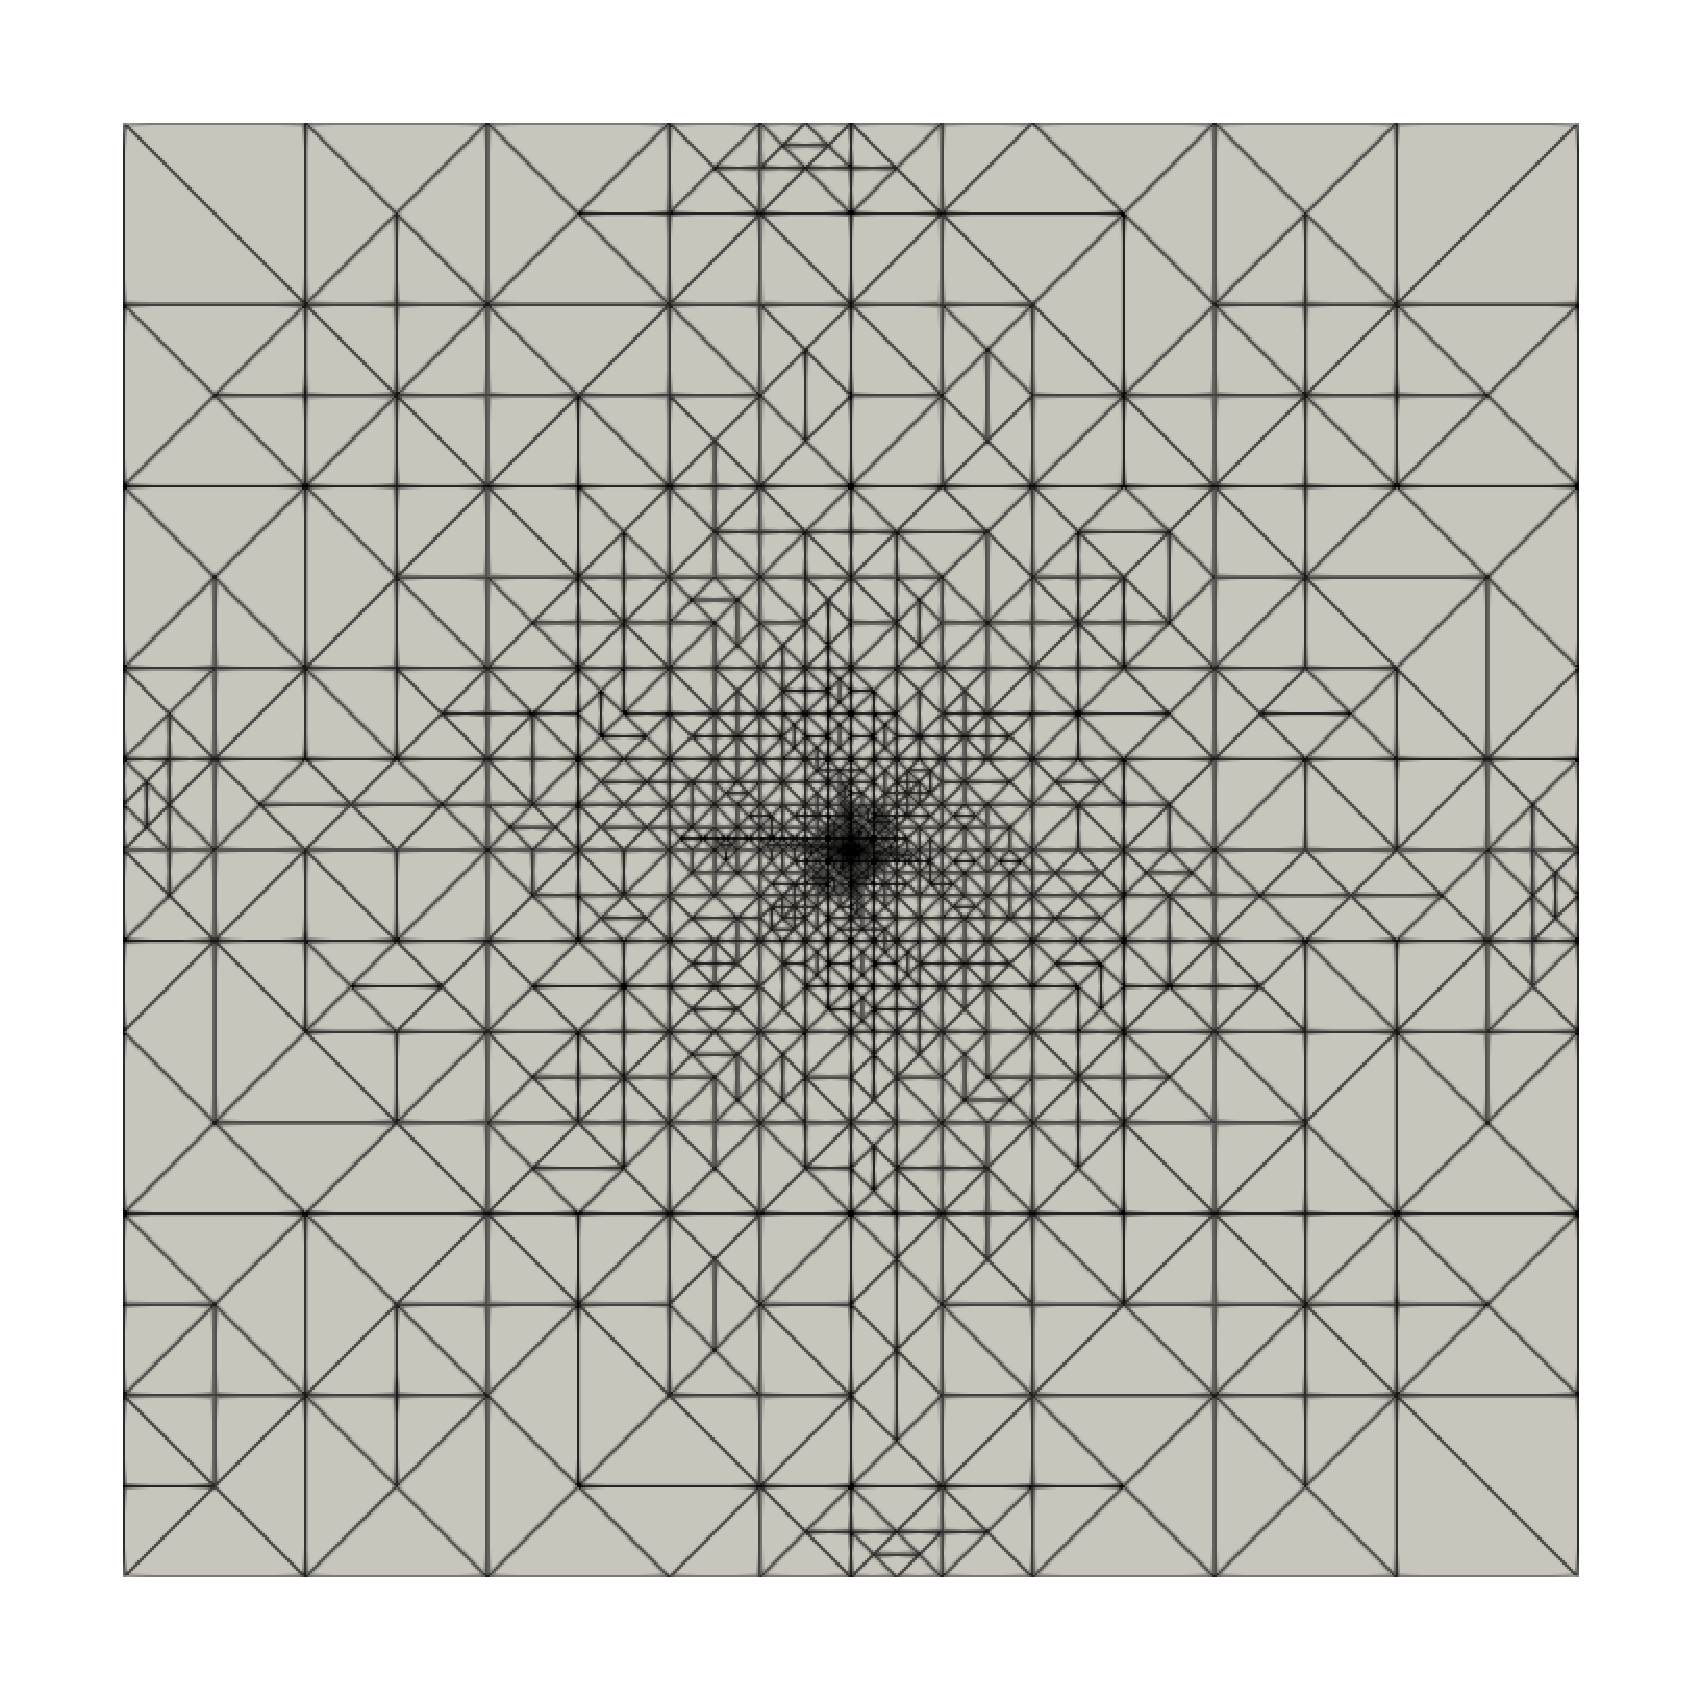
\includegraphics[width=\textwidth]{Riviere-100_P1_RT2_Mesh.pdf}
        \caption{}
        \label{fig:poisson-riviere_refmesh-p1}
    \end{subfigure}
    \hfill
    \begin{subfigure}[b]{0.32\textwidth}
        \centering
        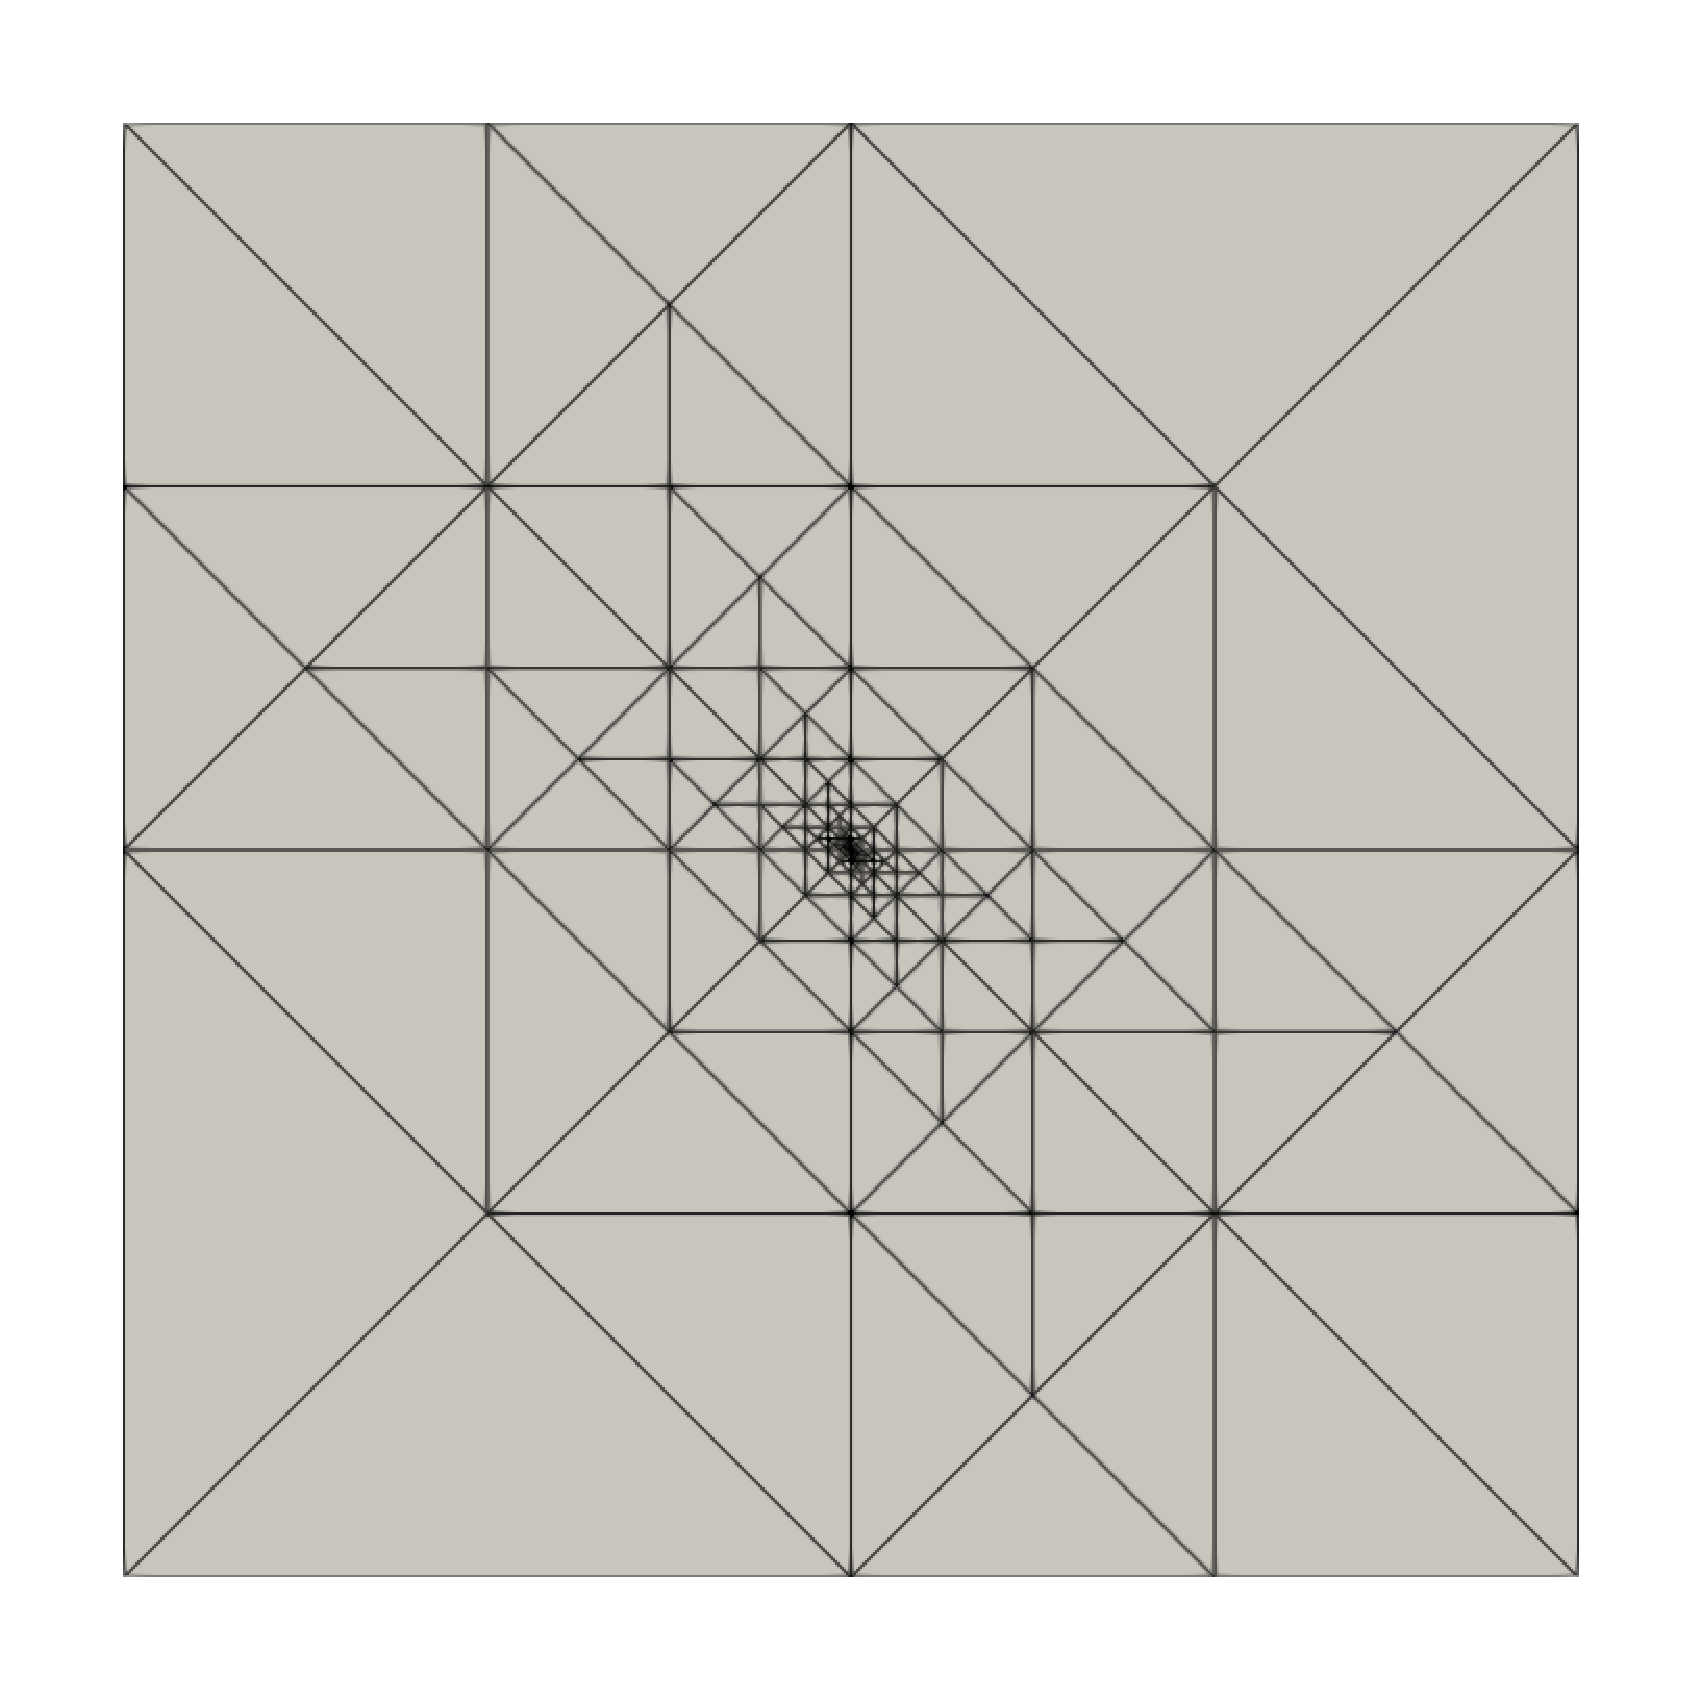
\includegraphics[width=\textwidth]{Riviere-100_P2_RT3_Mesh.pdf}
        \caption{}
        \label{fig:poisson-riviere_refmesh-p2}
    \end{subfigure}
    \caption{Results of adaptive FEM calculations with different orders $k$ and $m$. E.o.c and $\mathrm{i_{eff}}$ after the final refinement step are reported in (a).The two final meshes for $\kappa_1=100$ are depicted in (b) for $k=m-1=1$ and (c) for $k=m-1=2$.}
    \label{fig:poisson-riviere}
\end{figure}

\begin{wrapfigure}{r}{0.4\textwidth}
\centering
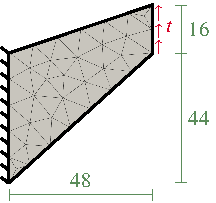
\includegraphics[scale=1.0]{fig_cooks-membrane.pdf}
\caption{Cooks membrane.}
\label{fig:cook_definition}
\end{wrapfigure}
\textbf{Example 2:} Based on the Poisson equation, the influence of the equilibration order $m$ on the efficiency of the resulting estimate is shown.
Using the Cooks membrane in Fig. \ref{fig:cook_definition}, this analysis is extended to linear elasticity, where the symmetry of the stress tensor is considered in a weak sense.
Within this analysis $\Pi_1=2.333$, $t=0.03$ and adaptive meshes based on a Dörfler marking strategy with $\theta=0.6$ are considered.
Characteristics of the first mesh fulfilling $\vert\vert\vert \Displacement - \Displacement_\h \vert\vert\vert \leq 10^{-3}$ are summarised in Fig. \ref{fig:cook_results-summary}. As $\LinPKEqlbH$ exactly fulfils the divergence condition from Definition \ref{def:equilibrated_stress}, $\eta$ reduced to the sum of the $\mathcal{A}$-norm of the stress difference $\LinPKEqlbH - \stressPKLin_\h$ and the norm of asymmetric part of $\LinPKEqlbH$. 
Following \ref{fig:cook_results-summary}, the estimate is clearly dominated by the second part.
Using equilibrated stresses of order $m=k+1$ increases the efficiency, with a relative reduction (compared to the case with $m=k$) comparable to those from the Poisson example.
An increased accuracy of the error estimate affects the effectivity of the adaptive solution procedure -- measured by the number of degrees of
freedom, required for a certain error -- in a positive way.
This trend is clearly much more pronounced for $k=2$, whereby a similar accuracy is achieved with $47\%$ fewer degrees of freedom.
A practical shortcut -- equilibration for $m=k+1$ is significantly more expensive than for $m=k$ -- seems to be the heuristic error indicator
\begin{eqnarray}
    \eta = \norm{\LinPKEqlbH - \stressPKLin_\h}\; ,
    \label{eq:elasticity_heuristic-ei}
\end{eqnarray}
where no weak symmetry is enforced on $\LinPKEqlbH$.
This yields efficiency indices close to one (see Fig. \ref{fig:cook_results-summary}), and shows, comparing the convergence history in Fig. \ref{fig:cook_results-convhist}, slightly better results as the guaranteed estimate with $m=k+1$.
\begin{figure}
    \centering
    \begin{subfigure}[b]{0.4\textwidth}
        \begin{tabular}{@{}l|c|c|ccc|l@{}}
            \toprule
            $k$ & $m$ & $n_\mathrm{DOF}$ & $\mathrm{err}$ & $\eta$ & $\eta _\mathrm{as}$ & $\mathrm{i_{eff}}$ \\ \midrule
            2 & 2 & 34070 & $0.0009$ & $0.009$ & $0.009$ & $10.7$ \\
            2 & 3 & 23202 & $0.0010$ & $0.008$ & $0.007$ & $7.9$ \\
            3 & 3 & 6656  & $0.0009$ & $0.020$ & $0.016$ & $17.0$ \\
            3 & 4 & 7100  & $0.0007$ & $0.009$ & $0.009$ & $13.0$ \\ \midrule
            2 & $2^*$ & 27788 & $0.0008$ & $0.001$ & $-$ & $1.5$ \\
            2 & $3^*$ & 26538 & $0.0008$ & $0.001$ & $-$ & $1.2$ \\
            3 & $3^*$ & 5738  & $0.0009$ & $0.001$ & $-$ & $1.5$ \\
            3 & $4^*$ & 5996  & $0.0008$ & $0.001$ & $-$ & $1.2$ \\ \bottomrule
        \end{tabular}
        \vspace{1.1cm}
        \caption{}
        \label{fig:cook_results-summary}
    \end{subfigure}
    \hfill
    \begin{subfigure}[b]{0.58\textwidth}
        \centering
        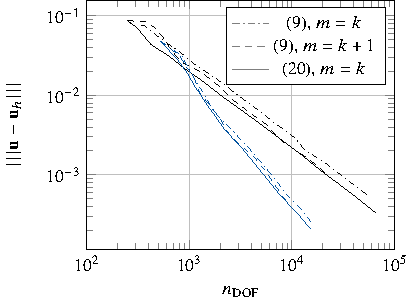
\includegraphics[scale=1.0]{fig_cook-convhistory.pdf}
        \caption{}
        \label{fig:cook_results-convhist}
    \end{subfigure}
    \caption{Effectivity of the different adaptive solution procedures for the Cooks membrane: (a) summarises the results for the first mesh with $\mathrm{err} = \vert\vert\vert \Displacement - \Displacement_\h \vert\vert\vert \leq 10^{-3}$, (b) details the convergence history (black: $k=2$, blue: $k=3$). Orders $m^*$ indicate the use of \eqref{eq:elasticity_heuristic-ei}}
    \label{fig:linelast-cook_results}
\end{figure}

Up to this point only the accuracy of the error estimates has been compared. 
Within the following the focus will be on the total solution time $t_\mathrm{tot}$, which is made up from $t_\mathrm{prime}$ -- the time for assembly and solution, using PETSc and MUMPS, of the primal problem -- and $t_\mathrm{eqlb}$, the time for performing the equilibration.
Comparing in a first step the relative equilibration costs $t_\mathrm{eqlb}/t_\mathrm{tot}$ for the Cooks membrane with fixed meshes in Fig. \ref{fig:cook_performance-uniform}, $t_\mathrm{eqlb}$ is -- for a sufficient size of the primal problem -- considerably smaller than $t_\mathrm{prime}$.  
Increasing $k$ increases the effort required for equilibration, while using an equilibration with $m=k+1$ is significantly more expensive than the respective lowest order case $m=k$. Similar timings for the adaptive solution of the Cooks membrane (timings are accumulated until $\vert\vert\vert \Displacement - \Displacement_\h \vert\vert\vert \leq 10^{-3}$) are summarised in Fig. \ref{fig:cook_performance-adaptive}.
While for the cases $k=m=2$ the total solution time is dominated by the solution of the primal problem, this trend is reversed for the more accurate (guaranteed) estimate with $k=m-1=2$.
Even though having the fewest primal degrees of freedom, the entire solution time is the highest due to the high computational costs for the equilibration.
Using primal approximations based on $k=3$ reduces the overall computation time, but leading to a significant share of the equilibration in the total computation time. 
An effect, amplified by the small sizes of the primal problems.
As for $k=2$ the heuristic indicator \eqref{eq:elasticity_heuristic-ei} with $m=k$ performs best, while the higher order estimate with $m=k+1$ is outperformed.
Clearly these results will have to be reevaluated in a parallel context -- which is beyond the current scope -- and also for primal problems of larger size.
\begin{figure}[]
\centering
    \begin{subfigure}[b]{0.6\textwidth}
        \centering
        \begin{tabular}{@{}c|ccc||c|ccc@{}}
        \toprule
        \multicolumn{4}{c}{$k=2$}    & \multicolumn{4}{c}{$k=3$}    \\ \midrule
        $n_\mathrm{DOF}\,\setminus\, m$ & 2    & $2^*$    & 3    & $n_\mathrm{DOF} \,\setminus\, m$ & 3    & $3^*$    & 4    \\ \midrule
        $3.49 \cdot 10^3$  & 36.3 & 27.4 & 66.4 & $3.31 \cdot 10^3$ & 45.4 & 37.9 & 63.1 \\
        $1.36 \cdot 10^4$  & 22.0 & 15.1 & 49.4 & $1.30 \cdot 10^4$ & 33.6 & 27.0 & 51.7 \\
        $2.14 \cdot 10^5$  & 15.3 & 10.2 & 38.6 & $2.04 \cdot 10^5$ & 24.5 & 19.3 & 40.9 \\
        $8.54 \cdot 10^5$  & 12.6 & 8.34 & 33.7 & $8.13 \cdot 10^5$ & 20.7 & 16.2 & 35.6 \\ \bottomrule
        \end{tabular}
        \vspace{0.2cm}
        \caption{}
        \label{fig:cook_performance-uniform}
    \end{subfigure}
    \hfill
    \begin{subfigure}[b]{0.38\textwidth}
        \centering
        \begin{tabular}{@{}l|c|ccc@{}}
            \toprule
            $k$ & $m$ & $t_\mathrm{prime}$ [s] & $t_\mathrm{tot}$ [s] & ratio [\%] \\ \midrule
            2 & 2     & $0.47$ & $0.61$ & 23.2\\
            2 & $2^*$ & $0.38$ & $0.45$ & 16.4\\
            2 & 3     & $0.31$ & $0.65$ & 52.7 \\ \midrule
            3 & 3     & $0.09$ & $0.15$ & 41.9\\
            3 & $3^*$ & $0.07$ & $0.11$ & 35.6\\
            3 & 4     & $0.10$ & $0.26$ & 60.5\\ \bottomrule
        \end{tabular}
        \caption{}
        \label{fig:cook_performance-adaptive}
    \end{subfigure}
    \caption{Performance measurements based on the Cooks membrane. (a) $\mathrm{ratio} = t_\mathrm{eqlb} / t_\mathrm{tot}$ in $\%$ for different primal problems. (b) Accumulated timings using an adaptive algorithm until $\vert\vert\vert \Displacement - \Displacement_\h \vert\vert\vert \leq 10^{-3}$. Orders $m^*$ indicate the use of \eqref{eq:elasticity_heuristic-ei}.}
    \label{fig:linelast-cook_performance}
\end{figure}

\section*{Conclusions}
Within this contribution dolfinx\_eqlb, a FEniCSx based library for the efficient equilibration of fluxes and stresses, has been introduced. 
Characteristic examples for the Poisson problem and linear elasticity highlight the applicability of the library.
Additionally, an efficient, but heuristic error indicator for elasticity is introduced, neglecting the asymmetry of the equilibrated stress.
Within our future work the efficiency of the presented implementation as well as the heuristic error indicator for real world problems has to be proven. 
We further intend to generalise the implementation to 3D domains and multi-physical problems like poroelasticity.
\vspace{-0.1cm}
\subsection*{Supplementary material}
This work is based on dolfinx\_eqlb v1.2.0 (\url{https://github.com/brodbeck-m/dolfinx_eqlb/tree/v1.2.0}). 
The presented examples can either be accessed via GitHub (\url{https://github.com/brodbeck-m/AFEM-by-Equilibration}) or, containing a Docker image, \cite{DatsetPaper}.
\vspace{-0.1cm}
\bibliographystyle{spbasic}
\bibliography{chapters/brodbeck/bibliography.bib}



% Write the full path to the location of the graphics relative to book.tex
\graphicspath{{chapters/habera/graphics/}}

% \linenumbers

\title{The FEniCS Project on AWS Graviton3}
\titlerunning{The FEniCS Project on AWS Graviton3}

\author{M.~Habera and J.~S.~Hale}
\authorrunning{Habera and Hale}

\institute{M.~Habera \email{michal.habera@rafinex.com} \at Rafinex SARL, Luxembourg and Institute of Computational Engineering, Department of Engineering, Faculty of Science, Technology and Medicine, University of Luxembourg, Luxembourg.\\
J.~S.~Hale \email{jack.hale@uni.lu} \at Institute of Computational Engineering, Department of Engineering, Faculty of Science, Technology and Medicine, University of Luxembourg, Luxembourg.}

\maketitle

\abstract{ARM architecture central processing units are increasingly prevalent
in high performance computers due to their energy efficiency, scalability and
cost-effectiveness. The overall goal of this study is to evaluate the
suitability of ARM-based cloud computing instances for executing finite element
computations. Specifically, we show performance results executing the FEniCS
Project finite element software on Amazon Web Services (AWS) c7g and c7gn
instances with Graviton3 processors. These processors support ARMv8.4-A
instruction set with Scalable Vector Extensions (SVE) for Single Instruction
Multiple Data operations and the Elastic Fabric Adaptor for communications
between instances. Both clang 18 and GCC 13 compilers successfully generated
optimized code using SVE instructions which ensures that users can achieve
optimized performance without extensive manual tuning. Testing a distributed
memory parallel DOLFINx Poisson solver with up to 512 Message Passing Interface
processes, we found that the performance and scalability of the AWS instances
are comparable to a dedicated AMD EPYC Rome cluster installed at the University
of Luxembourg. These findings demonstrate that ARM-based cloud computing
instances, exemplified by AWS Graviton3, can be competitive for distributed
memory parallel finite element analysis.}

\section*{Introduction}

The FEniCS Project~\citep{alnaes2015fenics,baratta_dolfinx_2023} has been used
to write finite element solvers for problems arising in fields that involve the
solution of partial differential equations (PDEs), including mathematics,
biology, physics, engineering, geophysics and mechanics.

Exploring ARM-based processors and cloud computing instances for executing
FEniCS Project-based solvers is worthwhile due to ARMs potential advantages in
cost-effectiveness, energy efficiency and scalability with respect to
x86-64-based machines~\cite{simakov_are_2023,suarez_comprehensive_2024}.
Examples of adoption of ARM in the HPC space include the Isambard project
(Isambard 3, NVIDIA Grace, \citep{isambard}), Mont-Blanc project (Phase 3,
Cavium Thunder X2, \citep{Rajovic2016}), Fugaku supercomputer (Fujitsu A64FX,
\citep{fugaku}) and Astra supercomputer (Cavium Thunder X2, \citep{astra}). The
publically available cloud services with ARM instances include Amazon Web
Services (AWS) (Graviton3 CPU based on Neoverse V1 and Graviton4 CPU with
Neoverse V2), Google Cloud (Axion CPU based on Neoverse V2,
\citep{google_arm_compute}) and Microsoft Azure (Azure Cobalt 100 based on
Neoverse N2, \citep{microsoft_azure}).

AWS Graviton3-based instances aim to provide cost effective compute resources
for scientific computing and machine-learning applications by including both
Scalable Vector Extension (SVE) instructions for Single Instruction Multiple
Data (SIMD) parallelism and the Elastic Fabric Adaptor (EFA) interconnect for
high-bandwidth low-latency communication between instances. This makes the AWS
cloud offering particularly appealing for executing scientific computing codes,
like the FEniCS Project.

A key technology in the FEniCS Project is the use of automatic code generation
(compilation). The user expresses their finite element problem in the Unified
Form Language (UFL)~\citep{alnaes_unified_2014} and then the FEniCSx Form
Compiler (FFCx)~\citep{kirby_compiler_2006} compiles the UFL description of the
problem into a low-level C kernel for computing the cell-local finite element
tensor.

One aspect of good performance of a compute-bound kernel is ensuring the
assembly code of the compiled kernel contains calls to Single Instruction
Multiple Data (SIMD) operations. SIMD operations can apply the same operation
to multiple data items in a single CPU clock cycle. For a recent overview of
SIMD programming strategies see e.g. \citep{rocke_evaluation_2023}. The current
strategy of FFCx with respect to SIMD is to ensure that its kernels are
amenable to the compiler applying automatic vectorisation, a process that
automatically converts a scalar program into a vectorised equivalent that uses
SIMD operations.
 
Consequently for users to achieve good performance when using FEniCSx on
Graviton3 it is important to verify that the latest compilers do automatically
emit SVE and/or Neon SIMD instructions when compiling the generated C finite
element kernels and that these kernels achieve reasonable runtime performance. 

In addition to SIMD parallelisation at the kernel level, DOLFINx, the finite
element problem solving environment of the FEniCS Project, also supports
distributed memory parallel assembly of global finite element data structures
(sparse matrices and vectors) using the Message Passing Interface (MPI), for
full details see \cite{baratta_dolfinx_2023}. For user's to run large-scale
DOLFINx simulations on AWS it is necessary to verify that the EFA interconnect
provides sufficient performance for parallel scalability.

In summary, the contribution of this chapter is to examine both SIMD
performance and multi-node parallel scaling of the FEniCS Project software on
Amazon's Graviton3 based instances. 

\section*{Methodology and results}

\subsection*{Systems}
AWS c7g and c7gn instances are compared to Aion computing instances available
at the University of Luxembourg HPC facilities \citep{VCPKVO_HPCCT22}. These
instances have different hardware configuration, see
\autoref{tab:aion-aws-config} for full details.

The FEniCS Project components are written in a mixture of Python, modern-style
C++20 and Standard C17. The Python interface is a wrapper around the core data
structures and computationally intensive algorithms written in C and C++.

\begin{table}
  \footnotesize
  \renewcommand{\arraystretch}{1.5}
  \begin{tabular}{l|l|l}
                              & Aion node                                                          & AWS c7g instance \\ \hline \hline
    Processor                 & \makecell[l]{2 x (AMD Epyc ROME 7H12, \\ 64 cores @ 2.6 GHz)}      & \makecell[l]{1 x (Graviton3, \\ 64 cores @ 2.6 GHz)} \\ \hline
    Architecture              & x86\_64, Zen 2 (AVX2)                                              & ARMv8.4-A, Neoverse V1 (SVE) \\ \hline
    Memory                    & \makecell[l]{256 GB DDR4 \\ 3200 MT/s = 25.6 GB/s \\ 8 NUMA nodes} & \makecell[l]{128 GB DDR5 \\ 4800 MT/s = 38.4 GB/s  \\ Unified Memory Access (no NUMA) } \\ \hline
    Total mem. bandwidth      & 2 x 200 GB/s                                                       & 1 x 300 GB/s  \\ \hline
  \end{tabular}
  \vspace{5pt}
  \caption{Configuration of the Aion nodes (University of Luxembourg HPC) and
	AWS c7g (Amazon) instances. The c7gn instance used in the Poisson weak
	scaling test has the same hardware as c7g with the addition of a
	$\SI{200}{\giga\byte\per\second}$ interconnect between instances for
	MPI-based communication.}
  \label{tab:aion-aws-config}
\end{table}

\subsection*{Memory bandwidth}

Low-order finite element methods are typically memory bandwidth constrained as
the time taken to load and store data from main memory (e.g. the mesh geometry)
dominates the time taken to perform the arithmetic operations to compute the
finite element cell tensor. Understanding the memory bandwidth characteristics
of a processor is therefore important for ensuring optimal performance.

STREAM \citep{McCalpin1995,McCalpin2007} is the industry standard benchmark for
measuring sustained memory bandwidth performance. They estimate memory bandwidth
from memory intense operations (copy, scale, add) on large contiguous arrays.

In \autoref{fig:stream-single} results for the copy operation for single-node
benchmark are shown. For the single-node benchmark $\SI{80}{\percent}$ of the
theoretical peak memory bandwidth of $\SI{400}{\giga\byte\per\second}$ for Aion
and $\SI{300}{\giga\byte\per\second}$ for AWS c7g is reached. This is considered
a reasonable outcome of the STREAM benchmark, \citep{McCalpin2023}. Bandwidth
saturation is observed at around $\SI{20}{\percent}$ of the node utilisation.
Both curves show different characteristics of the saturation point due to
different memory access configuration. On the Aion instances there are 8
non-unified memory access (NUMA) nodes of 16 cores each, while AWS c7g instances
are setup with unified memory access.

\begin{figure}
\begin{center}
        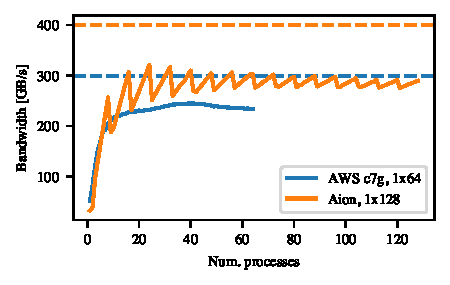
\includegraphics{chapters/habera/graphics/stream_plots/stream_single_node.pdf}
\end{center}
	\caption{Single-node STREAM benchmark. Theoretical peak bandwidth of each system show as dashed line.}
        \label{fig:stream-single}
\end{figure}

\subsection*{Finite element kernels}

In order to measure the performance of a standard FEniCS user finite element
code we used the Local Finite Element Operator Benchmarks repository
\citep{Baratta2023}. The benchmark measures execution time for local finite
element kernel generated by the FEniCS Form Compiler (FFCx) v0.9.0
\citep{kirby_compiler_2006}. We generate a matrix-free three-dimensional
Laplace kernel representing a finite element discretisation of the action of
Laplace operator $A_{ij}$ with spatially varying material property $\kappa(x)$
\begin{align}
    v_i = A_{ij} w_j, \quad
    A_{ij} = \int_K \kappa J_{mk} J_{mn} \nabla_k \phi_i \nabla_n \phi_j |\det J| \mathrm dx,
\end{align}
where $K$ is a fixed reference tetrahedron, $w_j \in \mathbb{R}^{n}$ is a
fixed, prescribed vector, $J$ is a Jacobian transformation matrix and $\phi$
are finite element basis functions.

The generated kernel calculates a double precision vector $v_i \in
\mathbb{R}^{n}$, where $n = 4$ for first-order discretization (low-order) and
$n = 165$ for eight-order discretization (high-order). Low-order kernels are
expected to be memory bandwidth limited, while high-order kernels have higher
arithmetic intensity. In addition, the matrix-free (operator action) version
requires fewer load and store operations in comparison to the assembly of a
matrix, increasing the ratio of floating-point operations to memory loads and
stores. Consequently for the high-order kernels there is the scope for
significant performance increases if the compiler can automatically emit SIMD
operations.

\subsubsection*{Generated code structure}

Compiler (loop) SIMD auto-vectorisation is usually performed for inner-most
loops with compile-time known bounds. The analysis of FFCx autogenerated code
is required to understand the potential and missed optimisations.

\lstset{style=CStyle}
\begin{lstlisting}[language=c,
    caption=Abbreviated FFCx generated finite element kernel.,
    basicstyle=\ttfamily\scriptsize,
    keywordstyle=\ttb\color{deepblue}\scriptsize,
    label=lst:c-code]
void kernel(double* restrict A, const double* restrict w, ...){
    // 1. Static arrays of basis functions and quadrature weights.
    // 2. Quadrature rule independent computations.

    for (int iq = 0; iq < NUM_QUAD_POINTS; ++iq) {
        // 3. Quadrature loop body.
        for (int ic = 0; ic < NUM_DOFS; ++ic){
            // 3.1 Coefficient evaluation.
            w1_d100 += w[4 + (ic)] * FE0_C0_D100_Q530[0][0][iq][ic];
            // ...
        }

        // 3.2 Scalar graph evaluation.
        double sv_530_0 = w1_d100 * sp_530_18;
        double sv_530_1 = w1_d010 * sp_530_22;
        // ...

        for (int i = 0; i < NUM_DOFS; ++i) {
            // 3.3 Tensor assignment loop.
            A[(i)] += fw0 * FE0_C0_D100_Q530[0][0][iq][i];
            // ...
        }
    }
}
\end{lstlisting}

An abbreviated example of generated C code is shown in Code Listing
\ref{lst:c-code}. Firstly, there are arrays defining finite element basis
functions at quadrature points. These require no arithmetic operations.
Computations independent of the quadrature loop contain more intense arithmetic
operations (e.g. determinant of the Jacobian), but are executed only once.
Non-affine geometry would require evaluation of geometric quantities at each
quadrature point, which would increase the arithmetic intensity and yield more
opportunities for vectorisation.

The most performance critical part of the code is contained in the quadrature
loop body. For the eight-order Laplace operator there is
\lstinline{NUM_QUAD_POINTS = 214} and \lstinline{NUM_DOFS = 165}. There are two
inner-most loops: coefficient evaluation and tensor assignment. Both contain a
set of multiply-add operations which are candidates for automatic vectorisation
via fused multiply-add operations in both SVE (Graviton3) and AVX2 (AMD EPYC).

\subsubsection*{Experimental results}

For the finite element kernel benchmarks we compiled the kernels with
LLVM/clang 18.1.3 and GCC 13.2.0. Full details are given in
\autoref{tab:compilers-kernels}.

\begin{table}
    \centering
    \footnotesize
    \renewcommand{\arraystretch}{1.5}
    \begin{tabular}{l|l|l|l}
                                    & Compiler     & Aion                                                                                            & AWS c7g \\ \hline \hline
        Ofast, native, vectorized   & GCC 13.2.0   & \makecell[l]{-Ofast \\ -march=znver2 \\ -mtune=znver2}                                          & \makecell[l]{-Ofast \\ -mcpu=neoverse-v1} \\ \hline
                                    & clang 18.1.3 & \makecell[l]{-Ofast \\ -march=znver2 \\ -mtune=znver2}                                          & \makecell[l]{-Ofast \\ -mcpu=neoverse-v1} \\ \hline
        Ofast, native, no vec.      & GCC 13.2.0   & \makecell[l]{-Ofast \\ -march=znver2 \\ -mtune=znver2 \\ -fno-tree-vectorize}                   & \makecell[l]{-Ofast \\ -mcpu=neoverse-v1 \\ -fno-tree-vectorize} \\ \hline
                                    & clang 18.1.3 & \makecell[l]{-Ofast \\ -march=znver2 \\ -mtune=znver2 \\ -fno-slp-vectorize \\ -fno-vectorize}  & \makecell[l]{-Ofast \\ -mcpu=neoverse-v1 \\ -fno-slp-vectorize \\ -fno-vectorize} \\ \hline
        O2, no vec.                 & GCC 13.2.0   & \makecell[l]{-O2 \\ -fno-tree-vectorize}                                                        & \makecell[l]{-O2 \\ -fno-tree-vectorize} \\ \hline
                                    & clang 18.1.3 & \makecell[l]{-O2 \\ -fno-slp-vectorize \\ -fno-vectorize}                                       & \makecell[l]{-O2 \\ -fno-slp-vectorize \\ -fno-vectorize} \\ \hline
    \end{tabular}
    \vspace{5pt}
    \caption{Compiler versions and compilation flags used for finite element kernel benchmarks.}
    \label{tab:compilers-kernels}
\end{table}

Results for kernel benchmarks are shown in \autoref{fig:local-deg1}
and \autoref{fig:local-deg8}. Low-order kernels (\autoref{fig:local-deg1}) show no
dependence on compiler vectorisation setup. On the other hand, AWS c7g shows
1.3x speed-up over Aion which we attribute to higher memory bandwidth for a
single process.

High-order kernels (\autoref{fig:local-deg8}), which are expected to benefit from
SIMD operations, show a clear link between compiler settings and performance.
Both clang and GCC auto-vectorisers perform well, producing a noticeable
speed-up (\textgreater 2x) in the most optimised setting. The vectorisation
speed-up (\textgreater 4x) is more significant with the Aion nodes.

\begin{figure}
    \begin{subfigure}{.5\textwidth}
        \centering
        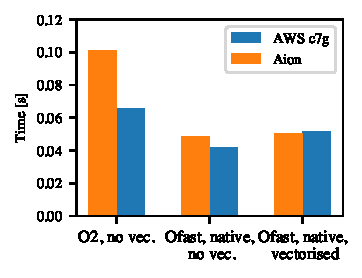
\includegraphics{chapters/habera/graphics/kernel_plots/local_operator_clang_deg1.pdf}
        \caption{clang 18.1.3.}
        \label{fig:local-clang-deg1}
    \end{subfigure}%
    \begin{subfigure}{.5\textwidth}
        \centering
        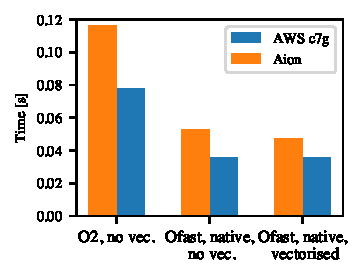
\includegraphics{chapters/habera/graphics/kernel_plots/local_operator_gcc_deg1.pdf}
        \caption{GCC 13.2.0.}
        \label{fig:local-gcc-deg1}
    \end{subfigure}
    \caption{Low-order Laplace operator action assembly.}
    \label{fig:local-deg1}
\end{figure}

\begin{figure}
    \begin{subfigure}{.5\textwidth}
        \centering
        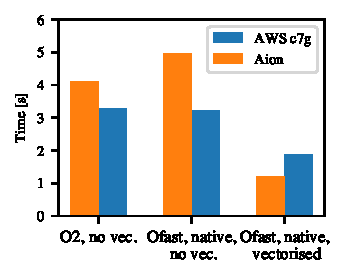
\includegraphics{chapters/habera/graphics/kernel_plots/local_operator_clang_deg8.pdf}
        \caption{clang 18.1.3.}
        \label{fig:local-clang-deg8}
    \end{subfigure}%
    \begin{subfigure}{.5\textwidth}
        \centering
        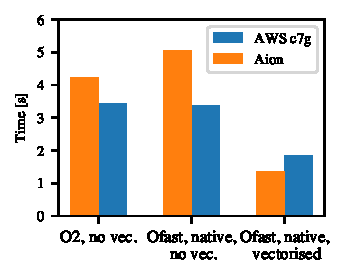
\includegraphics{chapters/habera/graphics/kernel_plots/local_operator_gcc_deg8.pdf}
        \caption{GCC 13.2.0.}
        \label{fig:local-gcc-deg8}
    \end{subfigure}
    \caption{High-order Laplace operator action assembly.}
    \label{fig:local-deg8}
\end{figure}

Optimisation reports (\texttt{-Rpass=loop-vectorize} for clang,
\texttt{-fopt-info-vec-optimized} for GCC) and the inspection of the generated
assembly reveal that the low-order operator action the compiler optimisation
level \lstinline{-Ofast} makes constant folding more effective and pre-computes
more operations at compile-time (e.g. partial sums of the static constant arrays)
\citep{GodboltArmClangDeg1}.

On Graviton3, both GCC and clang generate SVE FMLA instructions
\citep{ArmReferenceManual} for both the coefficient evaluation and tensor
assignment loops \citep{GodboltArmClang,GodboltArmGCC}. FMLA, or Floating-point
fused Multiply-Add, is a SIMD instruction that multiplies two vectors stored in
SVE registers and adds the result to a third vector. The coefficient evaluation
loop with no interdependencies between iterations is a perfect example for
compiler auto-vectorisation. Moreover, for coefficients of higher order
discretization, there is potential for exploiting wider SVE registers (up to
2048 bits).

An assembly excerpt for the coefficient evaluation is shown below.
\begin{lstlisting}[
    basicstyle=\ttfamily\footnotesize,
    keywordstyle=\ttb\color{deepblue}\footnotesize]
ld1d    {z0.d}, p0/z, [x7, x0, lsl #3]
ld1d    {z25.d}, p0/z, [x3, x0, lsl #3]
fmla    z3.d, p0/m, z25.d, z0.d
...
faddv   d1, p1, z1.d
\end{lstlisting}
As expected, there are two contiguous loads LD1D into two of the available SVE
Z0-Z31 registers followed by a fused Multiply-Add instruction. The result is
accumulated into an SVE register Z3 which is then horizontally summed outside
of the vectorised loop (FADDV). Here P0 is a predicate register without any
constraints on the available elements.

On Aion, both GCC and clang vectorise both coefficient evaluation and tensor
assignment loops and rely on the \lstinline{VFMADD231PD} instructions on the
YMM registers, i.e. vectorisation width of 4 doubles
\citep{Godboltx86Clang,Godboltx86GCC}.

\subsection*{Parallel scalability}

Results for the parallel scalability were produced using performance test codes
for FEniCSx \citep{Wells2023} built against DOLFINx 0.6.0 and PETSc 3.18
\citep{petsc} with the Spack package manager setup to use GCC 12.2.0. We setup
Spack to use a version of OpenMPI provided by AWS which includes the appropriate
libfabric with native support for the EFA interconnect. Libfabric is a network
communication library that abstracts networking technologies from fabric and
hardware implementation, ensuring optimal data transfer across Amazon's
proprietary EFA interconnect.

The Poisson equation solver benchmark consists of the following measured steps:
\begin{enumerate}
    \item Create mesh. Create a unit cube mesh and discretise using linear
    tetrahedral cells. Partition the mesh with Parmetis 4.0.3 partitioner
    \citep{Karypis1998} and distribute.
    \item Assemble matrix. Execute the local Poisson equation kernel over the
    mesh and assemble into a PETSc MATMPIAIJ (distributed compressed sparse row)
    matrix.
    \item Solve linear system. Run Conjugate Gradient (CG) solver with a classical algebraic
    multigrid (BoomerAMG \citep{hypre}) preconditioner.
\end{enumerate}
Creating the mesh (including partitioning), assembling matrices and solving the
resulting linear system are typically the most expensive steps in a finite
element solve. They also contain significant parallel communication steps that
can highlight issues in either the finite element solver, or the underlying MPI
hardware/software stack, leading to poor parallel scaling. 
%
Weak scaling results (constant workload of approx. \SI{5e+5} degrees-of-freedom
per process) are shown in \autoref{fig:weak-scaling}. Both Aion and AWS c7gn
show almost constant times for mesh creation ($< 5\%$ difference).

Matrix assembly is expected to have ideal weak parallel scalability due to the
cell-local nature of the assembly loop and negligible amount of MPI
communication during matrix finalisation. Aion and AWS c7gn show small increase
in time (10-15 \%) for 512 processes.

The time for the solve step increases by 40 \% for 512 processes on AWS c7gn and
by 27 \% on Aion. However, the number of Krylov iterations of the preconditioned
CG solver grows from 16 to 20 for 512 processes (25\% increase) due to the
inefficiency of the algebraic multigrid preconditioner on an unstructured 3D
mesh. Taking this into account, the time per iteration is almost constant on
Aion ($< 5\%$) and a small increase of 15 \% on AWS c7gn is observed.

\begin{figure}
    \begin{subfigure}{.7\textwidth}
	\begin{center}
        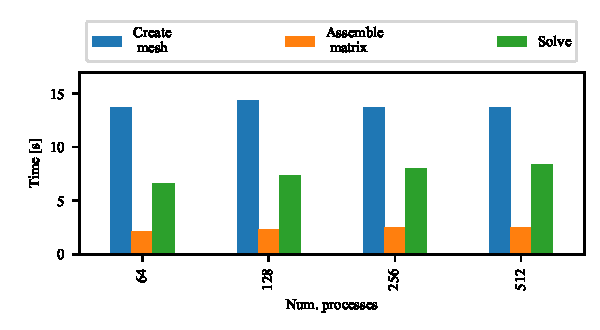
\includegraphics{chapters/habera/graphics/parallel_scaling_plots/output/weak_scaling_aion_poisson.pdf}
        \caption{Aion, \SI{5e+5} degrees-of-freedom per process, 25 \% utilisation (32 processes per node).}
        \label{fig:weak-scaling-aion}
	\end{center}
    \end{subfigure}

    \begin{subfigure}{.7\textwidth}
	\begin{center}
        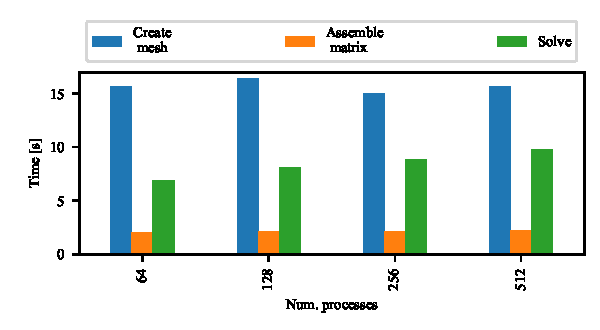
\includegraphics{chapters/habera/graphics/parallel_scaling_plots/output/weak_scaling_aws_c7gn_poisson.pdf}
        \caption{AWS c7gn, \SI{5e+5} degrees-of-freedom per process, 50 \% utilisation (32 processes per node).}
        \label{fig:weak-scaling-aws}
	\end{center}
    \end{subfigure}
    \caption{Weak parallel scalability of the DOLFINx Poisson equation solver on Aion and AWS c7gn systems.}
    \label{fig:weak-scaling}
\end{figure}

\section*{Conclusions}

Benchmarks for memory bandwidth, local finite element kernels and parallel
scalability of Poisson solver were executed on Aion nodes and on AWS c7g(n)
instances.

Memory bandwidth measured using STREAM MPI confirms higher memory transfer rate
of AWS c7g(n), but a superior total bandwidth of
~\SI{310}{\giga\byte\per\second} per Aion node.

In terms of auto-vectorisation capabilities of GCC 13.2.0 and clang 18.1.3, both
produced optimised instructions for the targeted microarchitectures (Zen 2 for
Aion and Neoverse V1 for AWS c7g). This observation was confirmed with
performance benchmarks based on local finite element kernels for the Laplace
operator.

The MPI-based distributed memory Poisson equation solver shows weak scaling with
15 \% time per iteration increase for 512 processes on the c7gn-based cluster.
Results for the in-house University of Luxembourg Aion system are slightly
superior with almost constant ($< 5 \%$ difference) time per iteration for 512
processes.

Based on our results, we conclude that AWS Graviton3 instances are a viable
alternative for high-performance computing tasks using the FEniCS Project
automated finite element solver. These instances are likely to be particularly
interesting for users with infrequent or highly elastic large-scale
computational demands~\cite{emeras_amazon_2016}.

In future work we plan to work on other more complex problems (e.g. linear
elasticity) and performance benchmarks of direct solvers. Additionally, the
latest generation Graviton4 instances provide an improved Neoverse V2
instruction set, which has a smaller SVE vector length of 128 bits,
\citep{ArmReferenceManualNeoverseV2}, which warrants further investigation.

\section*{Supplementary material}
Raw data and plotting scripts are archived at \citep{habera_2024_13748405}.

\begin{acknowledgement}
This project has received compute resources from Amazon Web Services (AWS)
through the first and second collaborative University of Luxembourg and
AWS Graviton3 call. The experiments presented in this paper were
carried out using the HPC facilities of the University of Luxembourg
~\cite{VCPKVO_HPCCT22} {\small -- see \url{https://hpc.uni.lu}}

This research was funded in whole, or in part, by the National Research
Fund (FNR), grant reference COAT/17205623. For the purpose of open
access, and in fulfillment of the obligations arising from the grant
agreement, the author has applied a Creative Commons Attribution 4.0
International (CC BY 4.0) license to any Author Accepted Manuscript
version arising from this submission.

JSH declares that he had a family member working at Rafinex during the period
of this project. This person was not involved in this study.
\end{acknowledgement}

\bibliographystyle{spbasic}
\bibliography{chapters/habera/bibliography.bib}
 
\graphicspath{{chapters/chp1/graphics/}}
\title{cuDOLFINx: A CUDA extension for FEniCSx}
\titlerunning{cuDOLFINx: A CUDA extension for FEniCSx}

\author{Benjamin~A.~Pachev, James~D.~Trotter, and Igor~A.~Baratta}
\authorrunning{Pachev et al.}
\institute{Benjamin.~A.~Pachev \email{benjmainpachev@utexas.edu} \at The University of Texas at Austin \\James.~D.~Trotter \email{james@simula.no} \at Simula Research Laboratory
\\Igor~A.~Baratta \email{ia397@cam.ac.uk} \at Department of Engineering, University of Cambridge
}


\maketitle

\abstract{Here we introduce cuDOLFINx---a Python package which extends FEniCSx with GPU-accelerated assembly capabilities. The extension enables FEniCSx codes to be accelerated on the GPU with minimal changes, and provides an easy path for researchers to experiment with GPU-accelerated PDE solvers. By constrast with previous efforts to enhance FEniCSx with GPU capabilities, cuDOLFINx is designed as a standalone package and does not require major changes to the core components of FEniCSx. Consequently, it has the potential to become a usable part of the FEniCSx ecosystem and a long-term solution to the problem of providing GPU acceleration capabilities in FEniCSx.
We further present performance benchmarks for representative GPU-accelerated FEniCSx applications on an NVIDIA GH200 GPU. Our results indicate that GPU-accelerated assembly routines within cuDOLFINx can be up to 40 times faster than traditional FEniCSx assembly with MPI parallelization on a multi-core CPU node.}

\section*{Introduction}
Graphics processing units (GPUs) provide an alternative means of parallelizing computations compared to a traditional clusters of multi-core CPUs. For many applications, GPUs are more energy efficient, thus having revolutionized fields such as machine learning~\citep{navarro2014survey}. Several well-known software packages used for solving PDEs have taken steps to provide GPU acceleration capabilities, including PETSc~\citep{MILLS2021102831}, MFEM~\citep{anderson2021mfem}, libCEED~\citep{abdelfattah2021gpu} and deal.II~\citep{arndt2021deal}.
However, GPU acceleration of PDE solvers has yet to become the norm, as other PDE libraries~\citep{baratta2023dolfinx,schoberl2014c++,hecht2012new,moxey2020nektar++,FiredrakeUserManual} lack support for GPU acceleration. Furthermore, even when GPU acceleration is available, it often has limited support and can be difficult to use. Modifying existing codes to use GPU parallelism remains a significant challenge~\citep{MILLS2021102831}. GPU programming requires a specialized compiler, memory space, and syntax, meaning that code must often be largely rewritten to take advantage of GPU acceleration.


A major attraction of FEniCSx~\citep{baratta2023dolfinx} as a tool for solving partial differential equations with the finite element method is its simple Python interface and automated generation of efficient C code. These features enable rapid prototyping and development of performant solvers for complicated PDEs. Our goal in developing cuDOLFINx \citep{cudolfinxzenodo} is to enable users of FEniCSx to add GPU acceleration to their existing PDE solvers with minimal effort.
GPUs are attractive for PDEs due to their increased throughput, floating point operations per second (FLOPS), and memory bandwidth. Although many PDEs are generally memory-bound, even memory-bound problems can benefit significantly from GPU acceleration. During the remainder of this chapter, we will give a brief overview of cuDOLFINx, present some example applications to the Poisson, Navier--Stokes, and shallow water problems, and finally discuss future development of cuDOLFINx.

\section*{Overview of cuDOLFINx}
The two most expensive steps in the finite element method are linear solves and the assembly of matrices or vectors. We would like to accelerate both of these steps with GPUs, in part to minimize expensive copies to and from GPU memory. Libraries such as PETSc~\citep{MILLS2021102831}, Ginkgo~\citep{ginkgo-toms-2022}, AMGx~\citep{naumov2015amgx}, hypre~\citep{li2020efficient,falgout2021porting}, SuperLU~\citep{li2023newly}, and others~\citep{lu2023tilesptrsv} provide efficient GPU-accelerated linear solvers. The goal of cuDOLFINx is to enable GPU-accelerated assembly, so that the entirety of FEniCSx finite element workflows can be GPU accelerated.

FEniCSx relies on auto-generated kernels to perform elementwise numerical integration, and the resulting element matrices or vectors can be assembled to form global matrices or vectors. In cuDOLFINx, these kernels are modified to execute on a GPU using CUDA. The generated kernels from FFCx are used as-is, with no GPU-targeted changes. Each element is processed by a single GPU thread, and atomic operations are used to prevent data races. This approach works well for low-order elements, but can be problematic for higher orders, as the computation of element stiffness matrices at high orders can require more local memory than is available to a single GPU thread. This can increase the usage of slower memory and reduce the number of GPU threads able to concurrently execute. Consequently, GPU assembly routines for high-order methods typically assign multiple threads to each element~\citep{MACIOL20101093,dziekonski2013generation,abdelfattah2021gpu, swirydowicz2019acceleration}. This is a goal of future work, and will require extending FFCx to support GPU parallelism within element kernels.

In addition to the elementwise kernels, cuDOLFINx provides GPU-based assembly loops to assemble the local contributions from each element into global matrices or vectors. This requires information about the mesh, boundary conditions, and function spaces to be copied to GPU memory. Internally, cuDOLFINx provides GPU counterparts for many of the data structures used in FEniCSx and automatically performs the data transfer to the GPU. Once data is transferred, it is expected to remain on the GPU, though mechanisms exist for moving data between the CPU and GPU when necessary.

The cuDOLFINx package extends the work of \cite{trotter2023targeting}. In addition to major modifications needed to support DOLFINx 0.9 (the most recent version at the time of writing), the following new features were developed:
\begin{enumerate}
    \item Support for boundary integrals was developed from scratch and considerably improved compared to the original version of the code, which only supported boundary integrals in very limited scenarios.
    \item To support DG methods, integrals on interior mesh edges are required. This functionality was added to the original GPU-accelerated code.
    \item Most of the users of FEniCSx utilize the Python version of the library. Consequently, a Python API was developed for the GPU-acceleration capabilities. It was designed to be much simpler to use than the original C++ interface, without loss of functionality.
    \item The GPU acceleration scheme has been applied to a wider range of problems, including the Navier-Stokes and shallow water equations.
\end{enumerate}

There are three main software components of cuDOLFINX. The first is a set of C++ classes containing CUDA data structures needed for assembly. These mirror corresponding DOLFINx classes (e.g. CUDAForm for Form, CUDAMesh for Mesh, etc.) and are responsible for copying the needed data to the GPU. The second consists of C++ classes which manage the generation, runtime compilation, and launching of CUDA assembly kernels. The final component contains the Python bindings for the C++ core. Most users will only need to utilize the Python wrapper. It provides Python versions of the C++ CUDA data structure classes, as well as convenience routines for performing assembly operations. We demonstrate its usage in the following section.

\section*{Sample usage}

Using cuDOLFINx within existing FEniCSx code requires only minor modifications. Consider the following example for solving Poisson's equation on the unit square:
\begin{python}
from mpi4py import MPI
from dolfinx import fem, mesh
import cudolfinx as cufem
from ufl import dx, inner, grad
import ufl

N = 1000
domain = mesh.create_unit_square(MPI.COMM_WORLD, N, N)
V = fem.functionspace(domain, ("Lagrange", 1))
f = fem.Function(V)
f.interpolate(lambda x: x[0]**2 + x[1])
u, v = ufl.TestFunction(V), ufl.TrialFunction(V)
A = -inner(grad(u), grad(v)) * dx
L = f * v * ufl.dx
\end{python}
Having defined a bilinear form \pythoninline{A} and linear form \pythoninline{L}, the following code creates CUDA counterparts of each form and a \pythoninline{CUDAAssembler} to offload the assembly of the matrix and right-hand side vector to a CUDA-enabled GPU:
\begin{python}
cuda_A = cufem.form(A)
cuda_L = cufem.form(L)
asm = cufem.CUDAAssembler()
mat = asm.assemble_matrix(cuda_A)
vec = asm.assemble_vector(cuda_L)
\end{python}
The assembled matrix and vector are provided in the form of \pythoninline{CUDAMatrix} and \pythoninline{CUDAVector} types, which can be readily converted to corresponding PETSc types for GPU-resident matrices and vectors. This transparently enables the use of PETSc's GPU-accelerated solver routines.


Offloading matrix or vector assembly to a GPU typically results in faster assembly, but it also incurs overheads due to copying necessary data structures to the device, as well as runtime compilation of CUDA assembly kernels. For large enough problems, the overhead is small compared to the assembly itself. Moreover, the overhead is incurred only once per form, and is therefore negligible for applications that require repeated assembly operations. Such use cases are very common and include time-dependent or nonlinear problems.

Below, we show how a simplified FEniCSx code for Newton iteration might be modified to support GPU acceleration. Boundary conditions are excluded for brevity---however, complete working examples with boundary conditions are available in the cuDOLFINX source code \citep{cudolfinxzenodo}. We take for our equation a nonlinear version of Poisson's equation with an extra cubic term in $u$. We begin by initializing PETSc data structures needed for assembly and linear algebra.
\begin{python}
from petsc4py import PETSc
use_cuda = True
u = fem.Function(V)
u_update = fem.Function(V)
residual = (f * v - inner(grad(u), grad(v)) + u**3 * v) * dx
jacobian = ufl.derivative(residual, u)

if use_cuda:
  # Force DOLFINx to use a CUDA PETSc vector
  u.vector.setType(PETSc.Vec.Type.CUDA)
  u_update.vector.setType(PETSc.Vec.Type.CUDA)
  asm = cufem.CUDAAssembler()
  residual, jacobian = cufem.form(residual), cufem.form(jacobian)
  L = asm.create_vector(residual)
  A = asm.create_matrix(jacobian)
else:
  residual, jacobian = fem.form(residual), fem.form(jacobian)
  L = petsc_fem.create_vector(residual)
  A = petsc_fem.create_matrix(jacobian)
\end{python}
The next step is to create the linear solver object. This requires a slight syntactical change when using cuDOLFINx to extract the underlying PETSc matrix from the assembled \pythoninline{CUDAMatrix}.
\begin{python}
ksp = PETSc.KSP().create(domain.comm)
ksp.setType("gmres")
ksp.getPC().setType("jacobi")
if use_cuda:
  # Get underlying PETSc Mat, as A is a CUDAMatrix
  ksp.setOperators(A.mat)
else:
  ksp.setOperators(A)
\end{python}
Finally, we reach the Newton iteration loop. Note the use of PETSc operations to add the computed Newton update to the solution, instead of vectorized numpy operations as is common in FEniCSx codes. This allows the computation to happen on the GPU, and is the reason for requiring that \pythoninline{u_update.vector} and \pythoninline{u.vector} be PETSc CUDA vectors.
\begin{python}
for i in range(5):
  if use_cuda:
    # by default entries are zeroed prior to assembly
    asm.assemble_matrix(jacobian, mat=A)
    A.assemble()
    asm.assemble_vector(residual, L)
    rhs = L.vector
  else:
    A.zeroEntries()
    petsc_fem.assemble_matrix(A, jacobian)
    A.assemble()
    L.array[:] = 0
    petsc_fem.assemble_vector(L, residual)
    rhs = L

  rhs.scale(-1)
  ksp.solve(rhs, u_update.vector)
  u.vector.axpy(1.0, u_update.vector)
\end{python}
A final step remains within the loop. The updated solution needs to be copied back to the underlying DOLFINx function, which resides on the host. This is not required for regular PETSc vectors, which share the same memory with the function object, but is a requirement for correctness in the case of CUDA type vectors, which use a separate GPU memory space.
\begin{python}
  if use_cuda:
    # Ensure host-side values of u match device-side values
    u.x.array[:] = u.vector.array
\end{python}

We will proceed to demonstrate the performance of cuDOLFINx for several representative use cases in which GPU acceleration can significantly enhance FEniCSx performance.

\section*{Performance evaluation}
We begin with two examples of the performance of the GPU assembly kernels in cuDOLFINx, and then present a use case of complete GPU offloading for both assembly and linear solves. All computations in the following experiments are performed in double precision. The primary hardware used in the following experiments is an NVIDIA GH200 Superchip, which consists of a Hopper GPU with 132 streaming multiprocessors (SMs) connected to a 72-core Grace CPU. The Hopper GPU has a memory bandwidth of 4 TB/s, while the CPU has a memory bandwidth of 384 GB/s~\citep{gh200specs}. Experiments were conducted using the Vista system at the Texas Advanced Computing Center (TACC).

\subsection*{Poisson}
Here we consider the problem of assembling a stiffness matrix for the solution of the Poisson equation on the unit cube. We use linear Lagrange finite elements on four different uniform, tetrahedral meshes ranging in size from about 1.3 to 16.5 million elements.  For each mesh, Table~\ref{tab:poisson_results} reports the throughput in millions of degrees of freedom per second (MDOF/s) for assembling the stiffness matrix with cuDOLFINx on a Hopper GPU and with DOLFINx on a Grace CPU.

Examining the results, the GPU doesn't appear fully saturated for the first two meshes, both of which have significantly fewer than one million degrees of freedom. This suggests that problems with approximately one million degrees of freedom or greater are needed to maximize the benefits of GPU acceleration. \cite{trotter2023targeting} reported a throughput of 189\,MDOF/s for the same problem using the ``Uniform 3'' mesh on an NVIDIA V100 GPU. In this study, we achieved a throughput of 376 MDOF/s on the GH200 GPU, roughly twice that of the V100. This result is expected, as the GH200 offers higher memory bandwidth and FLOPS. Further investigation will be conducted to explore the underlying factors behind these performance gains.
\begin{table}[t]
    \centering
\begin{tabular}{lrrrr}
\toprule
          &          &             & \multicolumn{2}{l}{Matrix Assembly} \\
                                     \cmidrule(lr){4-5}
Mesh      & Elements & DOFs        & Hopper (GPU) & Grace (CPU) \\
\midrule
Uniform 1 &  1,296,000 &   226,981 & 182.8 & 19.9 \\
Uniform 2 &  3,072,000 &   531,441 & 297.5 & 25.6 \\
Uniform 3 &  6,000,000 & 1,030,301 & 376.5 & 13.0 \\
Uniform 4 & 16,464,000 & 2,803,221 & 373.3 & 29.8 \\
\bottomrule
\end{tabular}
\caption{Performance of Poisson matrix assembly, in millions of DOFs per second.}
    \label{tab:poisson_results}
\end{table}

\subsection*{Shallow water}
For a more realistic example that also displays the complexity enabled by FEniCSx, we present assembly benchmarks using the variational forms in SWEMniCS~\citep{dawson2024swemnics}, a FEniCSx-based solver for the shallow water equations. SWEMniCS implements a suite of stabilized 2D shallow water solvers with implicit time stepping. Due to the nonlinearity of the shallow water equations, a Newton solver is required at each time step.

We investigated the efficiency of automatically generated CUDA assembly kernels for two stabilized schemes within SWEMniCS: the Discontinuous Galerkin (DG), and the Streamline Upwind Petrov-Galerkin (SUPG) schemes. The DG method uses broken test and trial spaces with a Lax-Freidrichs numerical flux. The DG scheme is more numerically stable, but requires more degrees of freedom than SUPG due to the use of discontinuous function spaces. For each scheme, we averaged the performance of both GPU and CPU assembly kernels over twenty Newton iterations for tidal flow simulations on square domains with uniform triangular meshes. Table~\ref{tab:swe_a100_vs_epyc} shows the speedup when using NVIDIA A100 GPU compared to a 64-core AMD Epyc 7763 CPU for assembling the Jacobian matrix and the residual vector for each scheme. The A100 GPU and Epyc CPU were both on the Lonestar6 system at TACC.
\begin{table}[t]
    \centering
    \begin{tabular}{lrrrrrrr}
\toprule
        &           &           \multicolumn{3}{c}{DG} & \multicolumn{3}{c}{SUPG} \\
                                  \cmidrule(lr){3-5}       \cmidrule(lr){6-8}
Mesh    &  Elements &  DOFs & Jacobian & Residual  & DOFs  & Jacobian & Residual \\
\midrule
Tidal 1 &   980,000 &  8,820,000 &     0.98 &      9.21 &  1,474,203 &   5.36 &     6.78 \\
Tidal 2 & 2,000,000 & 18,000,000 &     0.99 &     12.18 &  3,006,003 &   5.51 &     6.84 \\
Tidal 3 & 3,380,000 & 30,420,000 &     0.95 &      9.66 &  5,077,803 &   5.36 &     5.60 \\
\bottomrule
\end{tabular}
    \caption{Speedup of assembly kernels on an NVIDIA A100 GPU relative to a 64-core AMD Epyc CPU. Larger numbers indicate faster GPU runtime.}
    \label{tab:swe_a100_vs_epyc}
\end{table}


Interestingly, the speedups differ for each variational form. In the case of the DG scheme, assembly of the residual vector obtains a speedup of 9--12${\times}$, whereas assembly of the Jacobian on the A100 GPU is comparable in performance to that of the 64-core AMD Epyc CPU. The SUPG scheme, on the other hand, obtains a consistent speedup of 5--7${\times}$ for both residual and Jacobian matrix assembly.

Using NVIDIA's Nsight Compute profiler, we can better understand the difference in performance between DG and SUPG.
Profiler results for the ``Tidal 3'' testcase are presented in Table \ref{tab:tidal_prof}. The profiler reports \textit{occupancy}, which indicates the percentage of active threads on the GPU relative to the total GPU thread capacity. Occupancy can be limited by the resources needed per thread, such as shared memory or registers. It can also be impacted by excessive branching or other kernel design flaws. In our case, the generated assembly kernels required a high number of registers, which limited the occupancy to under 20\,\%. However, both the DG and SUPG kernels are able to utilize a large fraction of the device throughput---memory in the case of DG and compute in the case of SUPG.

To further understand the difference in performance between SUPG and DG, we used the Nsight Compute profiler to obtain the \textit{arithmetic intensity} for both Jacobian assembly kernels, which is the ratio of FLOPS performed to bytes of memory accessed. The arithmetic intensity is 0.22 FLOPS/byte for SUPG and 0.1 FLOPS/byte for DG, which partly explains why SUPG achieves higher compute throughput than DG.

Ultimately, the deciding factor in which method is more suitable for GPU offloading is the speedup factor relative to the CPU. By this criteria, SUPG is better in an implicit time stepping context where matrix assembly is required. However, for an explicit time stepping method, only vector assembly is required, and so DG will perform better on the GPU.
\begin{table}[t]
    \centering
\begin{tabular}{llrrrr}
\toprule
Method & Kernel & \begin{tabular}{@{}l}Theoretical\\ Occupancy\end{tabular} & \begin{tabular}{@{}l}Achieved\\ Occupancy\end{tabular} & \begin{tabular}{@{}l}Memory\\ Throughput\end{tabular} & \begin{tabular}{@{}l}Compute\\ Throughput\end{tabular} \\
\midrule
DG   & Jacobian & 12.50\,\% & 12.33\,\% & 41.44\,\% & 10.43\,\% \\
DG   & residual & 18.75\,\% & 18.74\,\% & 64.97\,\% & 18.20\,\% \\
SUPG & Jacobian & 12.50\,\% & 12.33\,\% & 48.66\,\% & 59.31\,\% \\
SUPG & residual & 12.50\,\% & 12.39\,\% &  5.64\,\% & 77.85\,\% \\
\bottomrule
\end{tabular}
\caption{Profiling statistics for the GPU assembly kernels on a square mesh.}
    \label{tab:tidal_prof}
\end{table}

\subsection*{Navier--Stokes}

While matrix assembly is a crucial part of the finite element method, most solvers also require the solution of linear systems. To assess the practicality of offloading a typical FEniCSx code to the GPU, we modified an existing FEniCSx Navier--Stokes solver~\citep{dokkenipcs} to use cuDOLFINx. The modified solver is hosted in a forked Github repository \citep{pachevipcs}. The solver uses an incremental pressure correction scheme~\citep{dokken2019shape}, which requires three stages per time step. While each stage requires a linear solve and assembly of a vector, only the first requires reassembly of a stiffness matrix. Second-order Lagrange tetrahedral elements are used for the velocity field, and first-order Lagrange elements for the pressure field. The mesh is a refined version of the 3D channel with an obstacle used in the original code, and contained 1,995,628 tetrahedra with 355,319 vertices.

The same hardware is used for comparison as in the Poisson experiment---namely the Hopper GPU and Grace CPU within a GH200 Superchip. Average timing results over 100 time steps for each component of the solver are provided in Table \ref{tab:navier_stokes_results}.
\begin{table}[t]
    \centering
\begin{tabular}{clrrrr}
\toprule
      &                 & \multicolumn{2}{c}{Hopper (GPU)} & \multicolumn{2}{c}{Grace (CPU)} \\
                          \cmidrule(lr){3-4}               \cmidrule(lr){5-6}
Stage & Solver/preconditioner       & Assembly & Solve               & Assembly & Solve \\
\midrule
    1 & BCGS/Jacobi     &    0.348 &               1.601 &    0.906 & 6.339 \\
    2 & GMRES/BoomerAMG &    0.009 &               0.013 &    0.007 & 0.108 \\
    3 & CG/Jacobi       &    0.004 &               0.079 &    0.013 & 0.564 \\
\bottomrule
\end{tabular}
\caption{Runtime for each stage of the Navier--Stokes solver in seconds.}
    \label{tab:navier_stokes_results}
\end{table}
Overall, the CUDA-accelerated solver averaged 2.07\,s per time step, while the original solver took 7.89\,s per time step. The overall speedup is therefore a factor of 3.8${\times}$. While the solution time is dominated by the linear solve for the first stage, assembly comprised over 10\,\% of the total runtime for both the GPU and CPU codes.

We note that compared to the Poisson example, the speedup of assembly for the Navier--Stokes code is smaller. We hypothesize this is due to the use of second-order elements for the velocity field. Higher order elements are known to pose difficulties for the GPU offloading approach used within cuDOLFINx because the auto-generated GPU kernels can require a large number of registers. This results in a phenomenon known as \textit{register spilling}, in which the GPU kernels are forced to utilize global memory to store some local variables, which degrades performance. Solutions include reworking the generated code to better hide memory transfer latency, potentially by reducing register spillage or minimizing the use of local memory. Another approach is to assemble each element using multiple GPU threads so that can share resource. Both of these solutions would require substantial enhancements to FFCx, the form compiler within the FEniCS project. Nevertheless, the attained speedup for assembly with quadratic elements in this case is still significant.

\section*{Conclusion}
We have introduced cuDOLFINx, an add-on enhancement to FEniCSx which provides GPU-accelerated assembly routines. We've demonstrated that offloading assembly to a GPU can provide significant speedups compared to multi-core CPUs, particularly for first-order elements. The package has a simple Python interface, and can be utilized in FEniCSx codebases with little effort.

In the near future, we intend to add support for multiple GPUs. Subsequent efforts will focus on providing support for non-NVIDIA GPUs, as well as developing efficient kernels for assembly with high-order elements. Work is currently underway to expand the documentation and examples, as well as to create easily installable binary distributions.

\section*{Supplementary material}
The source code of cuDOLFINx is archived at \citep{cudolfinxzenodo}.

\begin{acknowledgement}
  We gratefully acknowledge the use of the Lonestar6 and Vista systems at the Texas Advanced Computing Center under the "ADCIRC" allocation.
  The research presented in this paper has benefited from the Experimental Infrastructure for Exploration of Exascale Computing (eX3), which is financially supported by the Research Council of Norway under contract 270053.
\end{acknowledgement}

\bibliographystyle{spbasic}
\bibliography{chapters/pachev/bibliography.bib}

% Write the full path to the location of the graphics relative to book.tex
\graphicspath{{chapters/marcibal/graphics/}} 

\title{Implementation of the Lam--Bremhorst \texorpdfstring{\(k\)-\(\varepsilon\)}{k-e} turbulence model in FEniCS}
\titlerunning{Implementation of the \texorpdfstring{\(k\)-\(\varepsilon\)}{k-e} turbulence model}

\author{Juraj Marcibál, Hans Joachim Schroll}
\authorrunning{J.~Marcibál, H.~J.~Schroll}

\institute{
J.~Marcibál \email{juraj.marcibal@gmail.com},
H.~J.~Schroll \email{achim@imada.dk} 
\at University of Southern Denmark, Department of Mathematics and Computer Science
}

\maketitle

% ---- Article starts here ---- 

% Abstract
\abstract{
In this paper, we give an overview of turbulence modeling and turbulence in general, followed by an implementation of the Lam--Bremhorst \(k\)-\(\varepsilon\) turbulence model in FEniCS \citep{alnaes2015fenics,baratta2023dolfinx}. We demonstrate how the model can be easily implemented in the latest version of FEniCS, even when working with the simplest methods and schemes. We hope this paper serves as a valuable resource for researchers and enthusiasts seeking a straightforward introduction to turbulence modeling and a practical guide for implementing models in FEniCS.
}

% Section 1 - Introduction
\section{Introduction and governing equations}

Turbulence is an ever-present phenomenon encountered in both natural environments and engineering systems, from airflow over an airplane wing to the movement of water in rivers. It occurs when fluid moves chaotically, irregularly and at a high Reynolds number, presenting challenges for study and applications \citep{wilcox_turbulence_2006}. 

\subsection{Literature review}

Turbulence modeling, including the \(k\)-\(\varepsilon\) model and implementation in FEniCS and other open-source software, has been covered in the literature before. The article by \cite{valen_implementing_2013} implements the model by \citep{launder_application_1974}, which is often regarded as the standard \(k\)-\(\varepsilon\) model, in FEniCS, providing an accessible introduction to turbulence modeling and FEniCS itself. However, the provided code is now over a decade old and only covers a simple channel flow case. 

On the other hand, \cite{mortensen_fenics-based_2011} present a more comprehensive turbulence modeling framework, implementing multiple models, including the Launder-Sharma \(k\)-\(\varepsilon\) model. While it extends beyond the turbulent channel flow example, the code is also incompatible with the latest version of Legacy FEniCS and its complexity makes it less approachable for newcomers.

This article aims to address the need for a clear up-to-date turbulence model implementation in the Legacy FEniCS. We demonstrate that implementing a turbulence model in the latest version is feasible, and satisfactory results can be obtained even when working with simple numerical schemes and simpler turbulence model. Additionally, we provide an introduction to turbulence and turbulence modeling, making this work a valuable starting point for researchers entering the field. 

\subsection{Modeling turbulence}

Consider the incompressible Navier--Stokes (NS) equations
\begin{equation}\label{eq: NS}
    \begin{split}
        \frac{\partial \mathbf{u}}{\partial t} + \mathbf{u} \cdot \nabla{\mathbf{u}}
        = 
        - \frac{1}{\rho} \nabla p + \nabla \cdot (\nu \nabla \mathbf{u}) + \mathbf{f},
        \\
        \nabla \cdot \mathbf{u}
        = 0,
    \end{split}
\end{equation}
where \(\mathbf{u}\), \(p\) are the instantaneous velocity and pressure, \(\mathbf{f}\) represents the external forces, \(\rho\) is the density and \(\nu\) is the molecular viscosity of the fluid. It is well known that solving Equation \eqref{eq: NS} numerically becomes difficult as Reynolds Number gets large. To accurately predict turbulent flow, we either need to work with a very fine mesh and small step-size, or resort to modeling. The former is often not feasible without a large computational power.

One approach to modeling turbulence is to consider not the instantaneous \(\mathbf{u}\) and \(p\), but rather the mean values \(\langle \mathbf{u} \rangle\) and \( \langle p \rangle\). By decomposing \(\mathbf{u}\) and \(p\) into their mean and fluctuating parts \(\mathbf{u} = \langle \mathbf{u} \rangle + \mathbf{u}'\) and \(p = \langle p \rangle + p'\), one can derive governing equations for the mean quantities. Such equations are called the Reynolds-Averaged Navier--Stokes (RANS) equations, and they take the form
\begin{equation}\label{eq: RANS}
    \begin{split}
        \frac{\partial \langle \mathbf{u} \rangle}{\partial t} + \langle \mathbf{u} \rangle \cdot \nabla{\langle \mathbf{u} \rangle}
        = 
        -\frac{1}{\rho} \nabla \langle p \rangle + \nabla \cdot (\nu \nabla \langle \mathbf{u} \rangle ) + \langle \mathbf{f} \rangle - \nabla \cdot \langle \mathbf{u}' \otimes \mathbf{u}' \rangle,
        \\
        \nabla \cdot \langle \mathbf{u} \rangle 
        = 0,
    \end{split}
\end{equation}
where \(\mathbf{R} := - \langle \mathbf{u}' \otimes \mathbf{u}' \rangle\) is the Reynolds stress tensor, often interpreted as describing the effect of turbulence on the mean flow \citep{wilcox_turbulence_2006}. It contains \(\mathbf{u}'\) which is not known nor solved for. The RANS equations are therefore not closed and \(\mathbf{R}\) needs to be modeled, usually using the hypothesis proposed by \cite{boussinesq__essai_1877}:
\begin{equation}\label{eq: Boussinesq hypothesis}
    \mathbf{R} 
    \approx 
    - \frac{2}{3}k \mathbf{I} 
    + \nu_t \left(\nabla{\mathbf{u}} 
    + (\nabla{\mathbf{u}})^T\right)
    \implies
    \nabla \cdot \mathbf{R} 
    \approx
    - \frac{2}{3} \nabla k 
    + \nabla \cdot \left( \nu_t \nabla \mathbf{u} \right),
\end{equation}
where \(\nu_t\) is the turbulent viscosity and \(k\) is the turbulent kinetic energy. Modeling turbulence now reduces to modeling \(\nu_t\) and \(k\), usually by solving additional transport equation or equations, one of them typically being a transport equation for \(k\).

\subsection{The Lam--Bremhorst \(k\)-\(\varepsilon\) model and boundary conditions}

The Lam--Bremhorst (LB) \(k\)-\(\varepsilon\) model \citep{lam_modified_1981} is one of the models proposed to close the RANS equations. It was chosen for its relative simplicity compared to the more popular models such as the model by \cite{launder_application_1974}. Formulated in Equation \eqref{eq: k-eps}, it supplements Equations \eqref{eq: RANS}, \eqref{eq: Boussinesq hypothesis} with two additional transport equations governing \(k\) and \(\varepsilon\) (dissipation of \(k\)). Together, these equations form a closed system that describes the mean behavior of turbulent flow.
\begin{equation}\label{eq: k-eps}
    \begin{split}
        &\frac{\partial \mathbf{u}}{\partial t} 
        + \mathbf{u} \cdot \nabla{\mathbf{u}}
        = 
        - \nabla{\left( \frac{1}{\rho}p + \frac{2}{3}k \right)}
        + \nabla \cdot \left[ (\nu + \nu_t) \nabla \mathbf{u} \right]
        + \mathbf{f},
        \\
        &\nabla \cdot \mathbf{u}
        = 0,
        \\
        &\frac{\partial k}{\partial t} 
        + \mathbf{u} \cdot \nabla{k}
        = \nabla \cdot \left[\left(\nu + \frac{\nu_t}{\sigma_k}\right) \nabla{k} \right]
        + P_k
        - \gamma k,
        \\
        &\frac{\partial \varepsilon}{\partial t} 
        + \mathbf{u} \cdot \nabla{\varepsilon}
        = \nabla \cdot \left[\left(\nu + \frac{\nu_t}{\sigma_\varepsilon}\right) \nabla{\varepsilon}\right]
        + C_1 f_1 P_k \gamma
        - C_2 f_2 \gamma \varepsilon,
        \\
        &\nu_t
        = C_\nu f_\nu \frac{k^2}{\varepsilon},
        \quad 
        P_k 
        = \mathbf{R} : \frac{1}{2} \left(\nabla{\mathbf{u}} + (\nabla{\mathbf{u}})^T\right),
        \quad
        \gamma
        = \frac{\varepsilon}{k},
        \\
        &f_\nu
        = (1 - \exp{\left( -0.0165 \text{Re}_k \right)})^2 \left(1 + \frac{20.5}{\text{Re}_\ell}\right),
        \quad
        f_1
        = 1 + \left( \frac{0.05}{f_\nu}\right)^3,
        \\
        &f_2 
        = 1 - \exp{\left(-\text{Re}_\ell^2\right)},
        \quad
        \text{Re}_k 
        = \frac{\sqrt{k} y}{\nu}, 
        \quad
        \text{Re}_\ell
        = \frac{k^2}{\nu \varepsilon},
        \\
        &C_\nu = 0.09, \quad
        C_1 = 1.44, \quad
        C_2 = 1.92, \quad
        \sigma_k = 1.0, \quad
        \sigma_\varepsilon = 1.3.
    \end{split}
\end{equation}
In Equation \eqref{eq: k-eps}, \(\mathbf{u}\) and \(p\) are the mean velocity and pressure (for better readability we no longer denote averages with \(\langle \cdot \rangle\)), \(k\) and \(\varepsilon\) are the turbulent kinetic energy and its dissipation, \(\rho\), \(\nu\) and \(\mathbf{f}\) are as in Equation \eqref{eq: NS}. Additionally, \(\nu_t\) is the turbulent viscosity, \(P_k\) and \(\gamma\) are the production and reaction terms of \(k\). 

On top of that \(f_\nu\), \(f_1\) and \(f_2\) are the damping functions, which solve the models' inability to predict flow near the wall \citep{greenshields_notes_2022}. Terms \(\text{Re}_k\) and \(\text{Re}_\ell\) are both referred to as the turbulent Reynolds numbers and \(y\) denotes the distance to the nearest solid wall. Lastly, \(C_\nu\), \(C_1\), \(C_2\) and \(\sigma_1\), \(\sigma_2\) are the experimentally determined model constants.

Since RANS and the NS are the same equations with different total pressure and total viscosity terms, they also have similar boundary conditions, hence we will only focus on boundary conditions for the equations governing \(k\) and \(\varepsilon\).

For \(k\) and \(\varepsilon\) consider the domain boundary \(\partial \Omega\) divided into disjoint subboundaries corresponding to solid walls, inflow and outflow. Natural boundary conditions for the outflow for both \(k\) and \(\varepsilon\) are the zero Neumann boundary conditions, i.e. \(\nabla k \cdot \mathbf{n} = 0\) and \(\nabla \varepsilon \cdot \mathbf{n} = 0\). For the solid wall \(k\) is set to zero, the boundary conditions for \(\varepsilon\) differs with different turbulence model, for the LB \(k\)-\(\varepsilon\) model we have \(\nabla \varepsilon \cdot \mathbf{n} = 0\). The inflow boundary conditions are most often estimated from the physical definitions of \(k\) and \(\varepsilon\):
\begin{equation*}\label{eq: definitions of k-e}
    k = \frac{3}{2} (U I)^2, 
    \quad
    \varepsilon = C_\nu \frac{k^{3/2}}{\ell},
\end{equation*}
where \(U\) is the average velocity magnitude, \(I\) is the turbulent intensity and \(\ell\) is the turbulent length scale. Both \(I\) and \(\ell\) are generally not known beforehand and need to be estimated. For estimation of \(I\) and \(\ell\) see \cite{greenshields_notes_2022}. These can then be implemented as Dirichlet boundary conditions in Legacy FEniCS.

\subsection{Non-dimensionalized quantities and the law of the wall}

In turbulence modeling, many results are formulated using the non-dimensionalized velocity magnitude (\(U^+\)), distance to the wall (\(y^+\)) and turbulent kinetic energy (\(k^+\)) given by:
\begin{equation}\label{eq: non-dimensionalized variables}
    U^+ := \frac{U}{U_\tau},
    \quad
    y^+ := \frac{y U_\tau}{\nu},
    \quad
    k^+ := \frac{k}{U_\tau^2},
\end{equation}
where \(U_\tau := \sqrt{\tau_\text{w}}\) is the so-called friction velocity and \(\tau_\text{w}\) is the so-called wall shear stress, in \(2\)D it is given by \( \tau_\text{w} := \left. \nu [\nabla (\mathbf{u} \cdot \mathbf{t})] \cdot \mathbf{n} \right\rvert_\text{wall} \), where \(\mathbf{n}\) and \(\mathbf{t}\) are the unit outward-facing normal and unit tangent vectors respectively. Note that in \(3\)D the definition of \(\tau_\text{w}\) is more complicated because of non-uniqueness of a tangent vector to the wall. We will however keep the test cases in this paper to \(2\)D only.

% Section 2 - Implementation
\section{Implementation}

In this section, we focus on the implementation of the LB \(k\)-\(\varepsilon\) model. We only outline the implementation of the transport equations for \(k\) and \(\varepsilon\), since the RANS equations can be solved using the same techniques as NS. In our case we used Chorin's splitting method together with Taylor-Hood elements to solve the transient version of RANS equations. For the steady state version, Picard iteration was used. 

\subsection{Weak formulation of the \texorpdfstring{\(k\)-\(\varepsilon\)}{k-e} transport equations}

To derive the weak formulation for the \(k\) equation, we first approximate the temporal derivative \(\partial k / \partial t\) by its finite difference approximation. The entire equation is then multiplied by a test function \(\varphi\). Lastly, the divergence theorem is applied to the diffusion term and zero Neumann boundary conditions are considered, resulting in Equation \eqref{eq: Transport equation for k}. The weak formulation then reads: at each time step \(n+1\) find \(k^{n+1} \in V_{k,\triangle} \subseteq V_k = H^1(\Omega)\) such that:
\begin{equation}\label{eq: Transport equation for k}
    \begin{split}
        &\int_{\Omega} \frac{k^{n+1} - k^n}{\Delta t} \varphi \dx 
        + \int_{\Omega} \left( \mathbf{u}^{n+1} \cdot \Grad k^{n+1} \right) \varphi \dx
        \\
        =
        - &\int_{\Omega} \left( \nu + \frac{\nu_t}{\sigma_k}\right) \Grad k^{n+1} \cdot \Grad \varphi \dx 
        + \int_{\Omega} P_k \varphi \dx 
        - \int_{\Omega} \gamma k^{n+1} \varphi \dx,
    \end{split}
\end{equation}
where \(V_{k, \triangle}\) is the finite element subspace of \(V_k\). The same can be performed for the \(\varepsilon\) transport equation. Both \(V_{k, \triangle}\) and \(V_{\varepsilon, \triangle}\) are spaces of piece-wise linear functions.

Terms \(\nu_t\), \(P_k\), \(\gamma\) and \(f_\nu, f_1, f_2\) are all sources of both non-linearity and coupling, as they all depend on both \(k\) and \(\varepsilon\). If we want to solve the equations separately, using linear solvers, it is most natural to treat all the terms above explicitly, i.e. to compute them using values from the previous time-step. 

\subsection{Further treatment of the equations}

As physical quantities, \(k\) and \(\varepsilon\) only attain positive values. However, the equations as of right now might produce negative values for both. The natural solution is to bound them from below by a small constant \citep{lew_note_2001}. To prevent instabilities, it is also advised to limit \(f_\nu\) to its physical bounds \citep{schimdt_two-equation_1988}:
\begin{equation*}\label{eq: Physical bound of fnu}
    f_\nu \longrightarrow \min(\max(0.01116225, f_\nu), 1.0).
\end{equation*}
It has been observed that the effect of \(k\) in the total pressure term is negligible when compared to the effect of pressure \(p\) or the viscous effects \citep{Ansys_Best_Practice}. On top of that, implementing the \(\nabla k\) term in the RANS equations often leads to instabilities. We therefore decided to omit the \(k\) term altogether from \(\mathbf{R}\):
\begin{equation*}\label{eq: Removing k from R}
    \mathbf{R} \longrightarrow \nu_t \left( \Grad \langle u \rangle + \left( \Grad \langle u \rangle \right)^T \right).
\end{equation*}
This results in a formulation which closer resembles ones found in the literature, as seen in articles by \cite{valen_implementing_2013} or \cite{greenshields_notes_2022}.

\subsection{Computational mesh and distance from the wall}

The \(k\)-\(\varepsilon\) model, as formulated in this article, solves the governing equations up to the solid walls. As we will see in the Results section, the turbulent quantities \(k\) and \(\varepsilon\) display large sensitivity and fluctuations in this region, especially in the region where the value of \(y^+\) is less than \(5\) (called the viscous sub-layer). It is essential that this behavior is captured by the model, therefore a mesh fine enough is required. 

Given a desired non-dimensionalized value \(d^+\), we can construct a mesh, such that for each element that lies on the solid wall, the non-dimensionalized distance \(y^+\) between the wall and the furthest point from the wall in the element is less than \(d^+\), by computing the actual distance \(y\) from Equation \eqref{eq: non-dimensionalized variables}. The problem is that the wall shear stress \(\tau_\text{w}\), used in Equation \eqref{eq: non-dimensionalized variables}, is in general not known beforehand and must be estimated. In short, for a pressure-driven turbulent flow, the wall shear stress can be estimated by plugging the solution for Hagen-Poiseuille flow into the definition of \(\tau_\text{w}\). For flow with prescribed inflow velocity profile see \citep{noauthor_cfd_nodate}.

For simple geometries, such as channel flow, the distance from the wall \(y\) can be computed explicitly. When working with more complex geometry, \(y\) must be estimated, for example by solving the so-called Eikonal equation.

% Section 3 - Results
\section{Results}

In this section, we present results obtained for two test cases, namely the fully developed turbulent channel flow and the flow around a backward-facing step. Complete datasets, meshes, codes, and one different case for further exploration are available on the GitHub page of one of the authors \href{https://github.com/joove123/k-epsilon}{https://github.com/joove123/k-epsilon}.

\subsection{Fully developed turbulent channel flow}

A fully developed turbulent channel flow is a high \(\text{Re}\) flow between two infinitely long plates, approximated with a finite mesh of length \(L\) by imposing periodic boundary conditions, separated by a distance \(2H\) as seen in Figure \ref{fig: fully developed turbulent channel flow}. Flow is driven by a constant negative pressure gradient in the direction of the flow, achieved by prescribing \(p\) on the inflow and the outflow as seen in Table \ref{tab: boundary conditions for the channel flow}. The relative simplicity of this essentially one-dimensional problem makes it a perfect test case for verification of the model. Even though the problem attains a steady solution, a transient solver was used to verify its implementation.

\begin{figure}[htbp]
    \centering
    \begin{tikzpicture}
        % Draw a rectangle with specified properties
        \draw[line width=1pt, fill=gray!20] (0.0,1.8) rectangle (6.0,1.9);
        \draw[line width=1pt, fill=gray!20] (0.0,0.0) rectangle (6.0,0.1);
        \draw[dashed, line width=1pt] (0,0.1) -- (0,1.9);
        \draw[dashed, line width=1pt] (6,0.1) -- (6,1.9); 
        
        \node at (2.6+0.3, 1.4) {\scriptsize Solid Wall};
        \node at (2.6+0.3, -0.35) {\scriptsize Solid Wall};
    
        \node at (-0.63, 1.2) {\scriptsize Periodic};
        \node at (-0.73, 0.85) {\scriptsize Inflow};
    
        \node at (7.15+0.15, 1.2) {\scriptsize Periodic};
        \node at (7.15+0.14, 0.85) {\scriptsize Outflow};
    
        % draw arrows
        \draw[<->, line width=0.75pt] (0.1, 0.35) -- (5.9, 0.35);
        \node at (3.0, 0.55) {\scriptsize $L$};
    
        \draw[<->, line width=0.75pt] (6.25, 0.1) -- (6.25, 1.8);
        \node at (6.55, 1.5) {\scriptsize $2H$};
        
    \end{tikzpicture}
    \captionsetup{width=0.85\textwidth}
    \caption{Computational domain for the turbulent channel flow.}
    \label{fig: fully developed turbulent channel flow}
\end{figure}

The simulation is operated at Reynolds number \(\text{Re}_H = 22000\) based on the half-channel height \(H\). However, in turbulence modeling and especially for the turbulent channel flow, the Friction Reynolds number (\(\text{Re}_\tau \)) given by \(\text{Re}_\tau := (U_\tau H) / \nu \) is often used as a measure of the flow. The simulation is operated at \(\text{Re}_\tau = 550\). 

\begin{table}
    \centering
    \begin{tabular}{m{2.1cm} m{1.75cm} m{1.75cm} m{1.75cm} m{1.75cm}}
        \hline
        & $\mathbf{u}$ & $p$ & $k$ & $\varepsilon$ \\
        \hline
        \textbf{Inflow} & periodic & $p=p_{\text{in}}$ & periodic & periodic \\
        \textbf{Outflow} & periodic & $p=p_\text{out}$ & periodic & periodic \\
        \textbf{Solid walls} & $0$ & $\nabla p \cdot \mathbf{n} = 0$ & $0$ & $\nabla \varepsilon \cdot \mathbf{n} = 0$ \\
        \hline
    \end{tabular}
    \captionsetup{width=0.85\textwidth}
    \caption{Boundary conditions for the turbulent channel flow.}
    \label{tab: boundary conditions for the channel flow}
\end{table}

To verify the accuracy of the model, numerical results are compared to a direct numerical simulation performed by \cite{lee_direct_2015}. The same simulation is conducted for a series of meshes with varying values of \(d^+\), ranging from \(16\) to \(0.5\) (smaller value indicates finer mesh), with results provided in Figure \ref{fig: channel flow profiles} (for better clarity, results corresponding to some values of \(d^+\) are not shown). 

\begin{figure}[htbp]
    \centering
    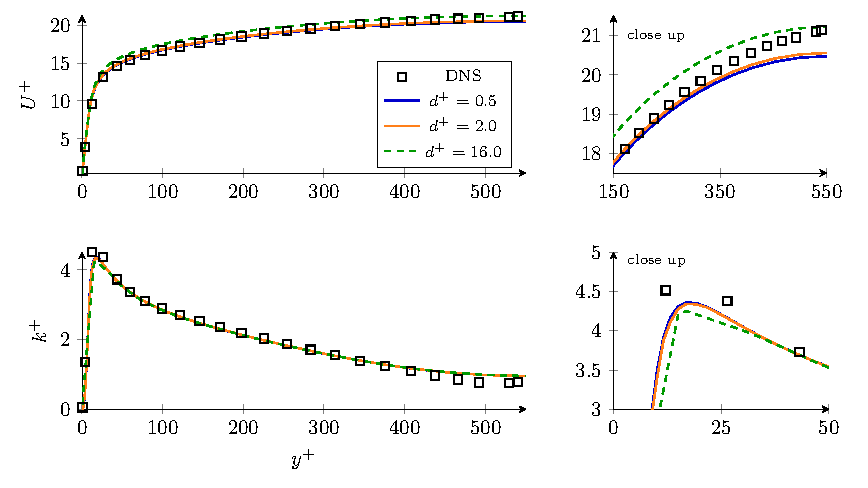
\includegraphics[width=0.825\textwidth]{channel flow-profiles.pdf}
    \captionsetup{width=0.85\textwidth}
    \caption{Comparison of velocity (top) and turbulent kinetic energy (bottom) profiles obtained on meshes with different resolutions with direct numerical simulation (left), together with close-up plots (right).}
    \label{fig: channel flow profiles}
\end{figure}

We feel, considering the solution profiles from Figure \ref{fig: channel flow profiles}, and the fact that the fields are most sensitive in the viscous sub-layer that a value of \(d^+ = 2\) strikes a good balance between computational efficiency and numerical accuracy. For this mesh in particular, number of elements in the mesh is \(864\). Velocity and pressure spaces have \(3480\) and \(511\) degrees of freedom respectively. On the other hand, both \(k\) and \(\varepsilon\) function spaces have \(438\) degrees of freedom. Since results for mesh with value \(d^+ = 2\) and \(d^+ = 0.5\) do not differ dramatically, the former value will also be used when constructing a mesh for the next flow case.  

\subsection{Flow over a backward-facing step}

Flow over a backward-facing step occurs when a fluid flows over a sudden expansion, creating a separated flow region and a complex re-circulation zone downstream of the step. Domain and boundary conditions are constructed such that they match the data from the experiment performed by \cite{driver_features_1985}. Both can be seen in Figure \ref{fig: backward facing step} and Table \ref{tab: boundary conditions for the backward facing step} respectively. This is a significantly more complex scenario than the channel flow, making it a perfect validation case for the model. Because of the mesh size, a steady-state solver was used to obtain the result.    

\begin{figure}[htbp]
    \centering
    \begin{tikzpicture}
    
        \fill[gray!20] (2.3,1.7) rectangle (8.0,1.8);
        \draw[solid,  line width=1pt]     (2.3,1.7) -- (8.0,1.7);
        \draw[solid,  line width=1pt]     (8.0,1.7) -- (8.0,1.8);
        \draw[solid,  line width=1pt]     (8.0,1.8) -- (2.3,1.8);
        \draw[solid,  line width=1pt]     (2.3,1.8) -- (2.3,1.7);
        
        \fill[gray!20] (2.3,0.0) rectangle (6,0.1);
        \fill[gray!20] (6,-0.45) rectangle (8,-0.35);
        \fill[gray!20] (6,-0.45) rectangle (6.1,0.1);

        \draw[solid,  line width=1.0pt]     (2.3,0.0) -- (6.0,0.0);
        \draw[solid,  line width=1.0pt]     (6.0,0.0) -- (6.0, -0.45);
        \draw[solid,  line width=1.0pt]     (6.0, -0.45) -- (8.0, -0.45);
        \draw[solid,  line width=1.0pt]     (8.0, -0.45) -- (8.0, -0.35);
        \draw[solid,  line width=1.0pt]     (8.0, -0.35) -- (6.1, -0.35);
        \draw[solid,  line width=1.0pt]     (6.1, -0.35) -- (6.1, 0.1);
        \draw[solid,  line width=1.0pt]     (6.1, 0.1) -- (2.3, 0.1);
        \draw[solid,  line width=1.0pt]     (2.3, 0.1) -- (2.3, 0.0);
    
        \draw[dashed, line width=1pt]     (1.,1.75) -- (2.3,1.75);
        \draw[dashed, line width=1pt]     (1.,0.05) -- (2.3,0.05);
        \draw[solid,  line width=1pt]     (1.,0.05) -- (1.,1.75);
        \draw[solid,  line width=1pt]     (8,-0.35) -- (8,1.7);
    
        % Add text labels
        \node at (2.15+2.0, 1.4) {\scriptsize Solid Wall};
        \node at (2.15+2.0, -0.3) {\scriptsize Solid Wall};
    
        \node at (1.65, 1.4) {\scriptsize Symmetry};
        \node at (1.65, -0.3) {\scriptsize Symmetry};
    
        \node[rotate=90] at (0.05, 1.) {\scriptsize Inflow}; 
        \node[rotate=90] at (8.95, 1.) {\scriptsize Outflow};
    
        % draw arrows
        \draw[<->, line width=0.75pt] (6.35, 0.1) -- (6.35, -0.3);
        \node at (6.55, -0.1) {\scriptsize $h$};
    
        \draw[<->, line width=0.75pt] (1.05, 0.35) -- (2.25, 0.35);
        \node at (1.65, 0.55) {\scriptsize $20h$};
        
        \draw[<->, line width=0.75pt] (2.3, 0.35) -- (6.1, 0.35);
        \node at (4.15, 0.55) {\scriptsize $110h$};
        
        \draw[<->, line width=0.75pt] (6.15, 0.35) -- (7.95, 0.35);
        \node at (7.025, 0.55) {\scriptsize $50h$};
    
        \draw[<->, line width=0.75pt] (8.25, -0.45) -- (8.25, 1.8);
        \node at (8.5, 1.) {\scriptsize $9h$};
    
        \draw[<->, line width=0.75pt] (0.75, 0.0) -- (0.75, 1.8);
        \node at (0.5, 1.) {\scriptsize $8h$};
        
    \end{tikzpicture}
    \captionsetup{width=0.85\textwidth}
    \caption{Computational domain for the flow over backward-facing step.} 
    \label{fig: backward facing step}
\end{figure}

The Reynolds number based on the step height \(h\) is approximately \(\text{Re}_h = 36000\), where the reference velocity used to compute \(\text{Re}_h\) is measured just before encountering the step, specifically at \(x = -4h\) (with the step located at \(x=0\)). Computational mesh consists of \(129 844\) elements. There are \(523 038\) and \(65 838\) degrees of freedom for velocity and pressure spaces respectively, and \(65 838\) for both \(k\) and \(\varepsilon\) spaces. 

\begin{table}
    \centering
    \begin{tabular}{m{2.1cm} m{1.75cm} m{1.75cm} m{1.75cm} m{1.75cm}}
        \hline
        & $\mathbf{u}$ & $p$ & $k$ & $\varepsilon$ \\
        \hline
        \textbf{Inflow} & $\mathbf{u}_{\text{in}}$ & $\nabla p \cdot \mathbf{n} = 0$
        & $k_{\text{in}}$ & $\varepsilon_{\text{in}}$
        \\
        \textbf{Outflow} & $\nabla \mathbf{u} \cdot \mathbf{n} = 0$ & $p=0$ 
        & $\nabla k \cdot \mathbf{n} = 0$ & $\nabla \varepsilon\cdot \mathbf{n} = 0$
        \\
        \textbf{Solid walls} & $0$ & $\nabla p \cdot \mathbf{n} = 0$ 
        & $0$ & $\nabla \varepsilon \cdot \mathbf{n} = 0$
        \\
        \textbf{Symmetry} & $\mathbf{u} \cdot \mathbf{n} = 0$ & $\nabla p \cdot \mathbf{n} = 0$ 
         & $\nabla k \cdot \mathbf{n} = 0$ & $\nabla \varepsilon \cdot \mathbf{n} = 0$
        \\
        \hline
    \end{tabular}
    \captionsetup{width=0.85\textwidth}
    \caption{Boundary conditions for the flow over backward-facing step.}
    \label{tab: boundary conditions for the backward facing step}
\end{table}

The model's accuracy is verified using experimental data from \cite{driver_features_1985}. A key measure of success is accurately predicting the reattachment point downstream of the step. This is determined by measuring the point \(\hat{x}\) where the skin friction coefficient (\(C_f\)) is equal zero. In the experiment, this was done using a laser oil-flow interferometer. Another measure for analyzing the results is the pressure coefficient (\(C_p\)). The results in Figure \ref{fig: backstep coefficients} show a poor match between the simulation and experiment, with the reattachment point observed at \(\hat{x} = 6.26 h\) compared to the simulation's \(\hat{x} = 5.0 h\). However, this discrepancy is expected from the \(k\)-\(\varepsilon\) model, which is known to struggle with separation and adverse pressure gradients. When compared to results in article by \cite{steffen_jr._critical_1993} with multiple versions of \(k\)-\(\varepsilon\) model, with reattachment points ranging from \(\hat{x} = 4.9\) to \(\hat{x} = 5.5\), we see a better match.

\begin{figure}[htbp]
    \centering
    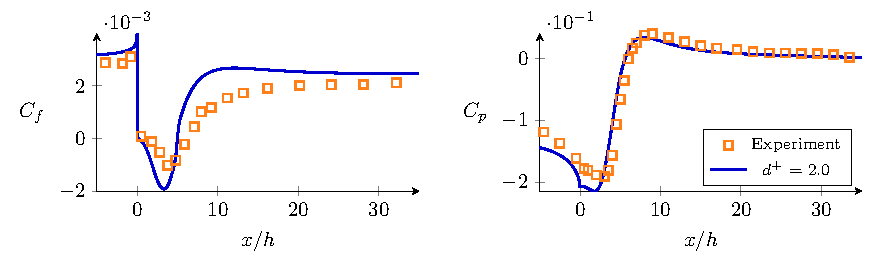
\includegraphics[width=0.825\textwidth]{backstep-coefficients.pdf}
    \captionsetup{width=0.85\textwidth}
    \caption{Comparison of the skin-friction coefficient (left) and the pressure coefficient (right) between experiment and simulation.}
    \label{fig: backstep coefficients}
\end{figure}

Figure \ref{fig: backstep profiles} presents normalized velocity magnitude \(U/U_\infty\) and \(k\) profiles at four points after the step. While the velocity profiles show good agreement, \(k\) diverges after \(x = 4h\), which is likely the cause of the reattachment point appearing prematurely. 

\begin{figure}[htbp]
    \centering
    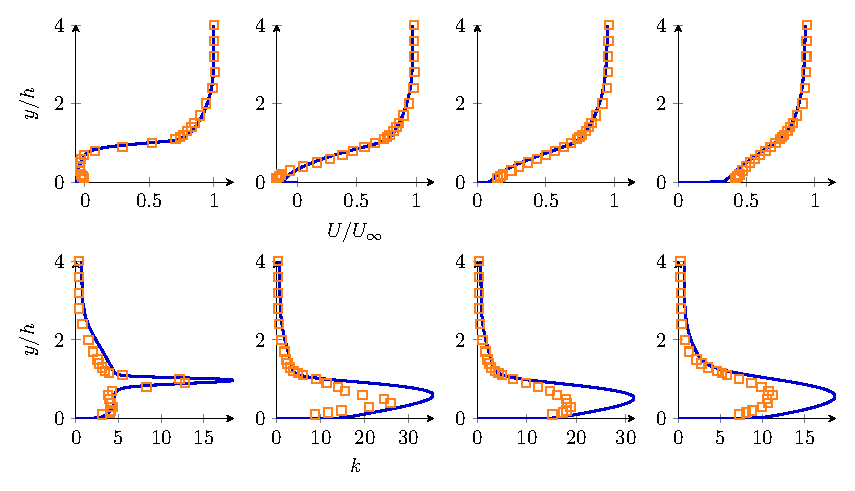
\includegraphics[width=0.825\textwidth]{backstep-profiles.pdf}
    \captionsetup{width=0.85\textwidth}
    \caption{Comparison of velocity (top) and turbulent kinetic energy (bottom) profiles at \(x = 1h\) (left), \(x = 4h\) (second left), \(x = 6h\) (second right) and \(x = 10h\) (right) between experiment and simulation.}
    \label{fig: backstep profiles}
\end{figure}

% Section 4 - Conclusion
\section{Conclusion}

The Lam--Bremhorst \(k\)-\(\varepsilon\) turbulence model was implemented successfully in FEniCS computing platform, both in the transient and steady-state formulation. We verified the implementation of the transient solver by simulating a fully developed channel flow, where a very good agreement was found between the computed solutions and the DNS. While the results of the backward-facing step simulation did not match the experiment, we still consider the implementation of the steady-state solver a success, as the results matched the expected behavior of the \(k\)-\(\varepsilon\) model. It is clear from those results that implementing the working \(k\)-\(\varepsilon\) model in FEniCS can be done with relative ease, and we do not see any reason why that would not be true for different turbulence models such as the \(k\)-\(\omega\) or the Spalart-Allmaras. These results can be replicated via scripts archived at \href{https://github.com/joove123/k-epsilon}{https://github.com/joove123/k-epsilon}.

\begin{acknowledgement}
    I would like to thank my master's thesis supervisor, Prof. Achim Schroll, for his professional guidance and support during the writing of my master's thesis and this article. I also thank NumFOCUS for the travel award that enabled me to attend the FEniCS 2024 conference. 
\end{acknowledgement}

% ---- Article ends here ---- 

\bibliographystyle{spbasic}

% Write the full path of your bibfile relative to book.tex
\bibliography{chapters/marcibal/bibliography.bib}

\graphicspath{{chapters/munthe/graphics/}}


\title{Growth and remodelling package in FEniCSx}

\author{Karl Munthe, Henrik N.T. Finsberg, Samuel T. Wall, Joakim Sundnes}

\institute{K. Munthe \at Simula Research Laboratory, Oslo, Norway and \\ Department of Informatics, University of Oslo, Norway, \email{karlfredrik@simula.no}
\and
H. Finsberg \at Simula Research Laboratory, Oslo, Norway
\and
S. Wall \at Simula Research Laboratory, Oslo, Norway
\and
J. Sundnes \at Simula Research Laboratory, Oslo, Norway and \\ Department of Informatics, University of Oslo, Norway}

\maketitle
\abstract{The heart is a dynamic organ that changes its size and shape to regulate its behaviour to the demands of the body, which can change for example through body growth, exercise, or the onset of a disease. Different models have been proposed to try to capture various types of cardiac growth resulting from mechanical stimuli, but the models have rarely been compared systematically. In this manuscript we present a framework implemented in FEniCSx that allows one to quickly run simulations of growth and remodelling with different material models and different growth laws. We present and compare the growth predicted by each model for a set of simple experiments, and compare the results to the relevant literature in the field. All the code can be found at \url{https://github.com/karlfm/Growth-and-Remodeling-in-FEniCSx}}
\vspace{12pt}
\section{Introduction}
In classical continuum mechanics one normally studies the mechanics of bodies where mass, linear momentum, angular momentum, and energy are conserved properties. This approach has been extremely successful and is the bedrock for traditional engineering disciplines, but it does not accurately capture aspects of how living organisms change with respect to their environment. One of the unique features of biological material is its ability to grow and evolve by adding or removing mass. Understanding how biological matter grows and what drives the growth is important, not only to understand normal growth and development, but also when and how growth may become non-compensatory and drive disease.\par It has been known for a long time that the growth of organs, such as the heart, is regulated at least in part by the forces applied to it \citep{Hsu1968}. This understanding has led to the formulation of growth laws that link growth and remodeling to local stress or strain. \par
In this chapter we will introduce a package written in FEniCSx that allows one to easily model growth and remodelling of biological tissue, with the aim of quickly testing combinations of growth models and material models. Allowing researchers to systematically test combinations of material models and growth tensors will aid in the discovery of more accurate models of growth and remodelling phenomena of biological tissue.
\section{Methods}
\subsection{Growth and remodeling in continuum mechanics}
Consider a solid body that is continuously and smoothly deforming from one configuration to another, and denote the initial configuration (also called the reference configuration) as $\mathcal{M}$ and the current configuration $\mathcal{N}$. We denote a point in $\mathcal{M}$ with uppercase letters $\mathbf{X} = (X, Y, Z)$ and a point in $\mathcal{N}$ with lowercase letters $\mathbf{x} = (x, y, z)$\footnote{Apart from the letters $X$, $Y$, and $Z$, all upper case letters represent tensors.}. A point in $\mathcal{M}$ can be mapped to a point in $\mathcal{N}$ by a motion, $\phi(\mathbf{X}): \mathbf{X} \rightarrow \mathbf{x}$, which is a diffeomorphism. We can map a vector from the reference configuration to the current configuration via the pushforward of $\phi$, which is commonly denoted by $\mathbf{F}$ and is referred to as the deformation gradient, computed as $\mathbf{F} = \partial\mathbf{x}/\partial\mathbf{X}$. The displacement field $\mathbf{u} = \mathbf{x} - \mathbf{X}$ is a vector field describing the displacement of each point $\mathbf{X}$ in the reference configuration to its location $\mathbf{x}$ in the deformed configuration. 
Most mechanical models of the heart assume that the tissue is hyperelastic, meaning that deformations of the material conserve its energy, and when any load on the tissue is removed it returns to its original reference shape. Growth, on the other hand, represents a permanent change of the unloaded reference configuration, and cannot be modeled as an elastic deformation. Instead, it is commonly modeled using the framework of plastic or elasto-plastic deformations. The most common approach, introduced by \citep{Rodriguez1994}, is to multiplicatively split the deformation tensor into an elastic part and an inelastic growth part, 
\begin{equation}
\label{eq: multiplicative split}
    \mathbf{F} = \mathbf{F}_e\mathbf{F}_g,
\end{equation}
where $\mathbf{F}_e$ is the elastic deformation and $\mathbf{F}_g$ is the plastic deformation that represents growth. 

One interpretation of \ref{eq: multiplicative split} is that the material first deforms by $\mathbf{F}_g$ in a way that does not cause stress, but might cause incompatibilities in the form of discontinuities or overlapping material. The deformation described by $\mathbf{F}_g$ leads to an unphysical intermediate configuration, which is then deformed by $\mathbf{F}_e$ in a way that removes the unphysical characteristics that occurred from $\mathbf{F}_g$, but adds residual stress. Sufficient conditions for the existence of intermediate configurations such as $\mathbf{F}_g$ are discussed in \citep{Goodbrake2021}. We assume that the deformation described by $\mathbf{F}_e$ is hyperelastic, such that we can obtain the first Piola–Kirchhoff stress tensor by differentiating a strain energy function,
\begin{equation}
\label{eq: stress}
    \mathbf{P} = \frac{\partial\Psi}{\partial \mathbf{F}_e}.
\end{equation}

We typically describe the growth in terms of multiple growth steps, given by
\begin{equation*}
    \mathbf{F}_g^{i + 1} = \mathbf{F}_g^i\mathbf{F}_g^\mathrm{inc} .
\end{equation*}
Here, $\mathbf{F}_g^\mathrm{inc}$ is the incremental growth tensor describing growth occuring in one step, and $\mathbf{F}_g^i$ is the cumulative growth after $i$ steps. The initial growth tensor, $\mathbf{F}_g^0$, is set to the identity tensor. The cumulative growth deformation tensor after $n$ steps is given by
\begin{equation*}
    \mathbf{F}_g^{n} = \mathbf{F}_{g}^\mathrm{inc}\vert_{t=0}\mathbf{F}_{g}^\mathrm{inc}\vert_{t=1} \cdots \mathbf{F}_{g}^\mathrm{inc}\vert_{t=n},
\end{equation*}  
where $\mathbf{F}_{g}^\mathrm{inc}\vert_{t=i}$ means the $\mathbf{F}_{g}^\mathrm{inc}$ at the $i$'th step. Note that the $i$'th incremental growth tensor is dependent on the stress or strain that occurred in the $i-1$'th growth step (see \citep{Goriely2007}). It is common to assume that the growth tensor is diagonal, and to express the incremental growth tensor in terms of fiber, crossfiber, and normal directions 
\begin{equation*}
    \mathbf{F}_g^\mathrm{inc} = F^\mathrm{inc}_{g,f}\mathbf{e}_f\otimes \mathbf{e}_f + F^\mathrm{inc}_{g,c}\mathbf{e}_c\otimes \mathbf{e}_c + F^\mathrm{inc}_{g,n}\mathbf{e}_n\otimes \mathbf{e}_n.
\end{equation*}
Here, $F^\mathrm{inc}_{g, i}$ for  $i = \{f, c, n\}$ are functions of either stress or strain, and $\mathbf{e}_i$ for $i = {\{f, c, n\}}$ are orthonormal basis vectors in the fiber, crossfiber, and normal directions respectively. 

The incremental growth tensor depends on the local stress or strain, which is determined by solving for mechanical equilibrium at each growth step; 
\begin{equation} \label{eq: system of equations}
\begin{aligned}
    \mathbf{F} & = \mathbf{F}_e\mathbf{F}_g && \text{in } \mathcal{M} ,\\
    \nabla\cdot\mathbf{P} & = 0 && \text{in } \mathcal{M}, \\
    \mathbf{P}\cdot \nu & = 0 && \text{on } \partial\mathcal{M}_N, \\
    \mathbf{u} & = g_D && \text{on } \partial\mathcal{M}_D,
\end{aligned}
\end{equation} 
where $\nu$ is a surface normal vector, $\partial\mathcal{M}_N$ and $\partial\mathcal{M}_D$ denote the boundaries which are prescribed Neumann and Dirichlet boundary conditions respectively. 

It remains to specify the growth laws that determine $F_g$ and the strain energy $\Psi$ in 
(\ref{eq: stress}). We will define the growth laws in the next section, but for all the 
experiments we use a nearly incompressible neo-Hookean model, so (\ref{eq: stress}) becomes
\begin{align*}
    \mathbf{P} &= \frac{\partial\Psi_\text{iso}}{\partial \mathbf{F}_e} + \frac{\partial\Psi_\text{vol}}{\partial \mathbf{F}_e}, \\
    \mathbf{P} &= \frac{\partial}{\partial \mathbf{F}_e}\left[\frac{\mu}{2}\left(\mathrm{tr}\mathbf{\bar{C}} - 3\right) + \kappa(J-1)^2\right],
\end{align*}
where $\mu$ and $\kappa$ material parameters. $\Psi_\text{iso}$ and $\Psi_\text{vol}$ are the isochoric (distortional) and volumetric (dilational) parts of the strain energy function. To decouple the energy stored in the body as a result of volume preserving deformation and non-volume preserving deformation, we introduce $\mathbf{\bar{F}}_e = \mathbf{F}_eJ^{-1/3}$, whose determinant is equal to one. The isochoric right Cauchy-Green deformation tensor, $\mathbf{\bar{C}}$, is calculated as $\mathbf{\bar{C}} = \mathbf{\bar{F}}_e^\top \mathbf{\bar{F}}_e$. Now, $\partial\Psi_\text{iso}/\partial \mathbf{F}_e = 0$ only if the deformation preserves the shape, and $\partial\Psi_\text{vol}/\partial \mathbf{F}_e = 0$ only if the deformation preserves the volume (see Chapter 6 of \citep{Holzapfel2002} for more details). \par 
For further information about continuum mechanics we recommend \citep{Marsden1983} and \citep{Holzapfel2002}, and for further information about growth and remodelling we recommend \citep{Goriely2017} and \citep{Yavari2010}.

\subsection{Numerical implementation}
 
Algorithm \ref{alg:growth_deform} shows an overview of the steps involved in the solution
of the growth model equations. For stress based growth, you would update the stress tensor rather than the strain tensor, and for additive growth laws, you would add the cumulative and incremental growth tensors instead of multiplying them together. \par
\begin{algorithm} 
    \caption{Growth tensor and stress/strain tensor are updated at each growth step. Both $\mathbf{F}_\mathrm{e}$ and $\mathbf{F}_g^\mathrm{inc}$ are dependent on $\mathbf{u}$.}\label{alg:growth_deform}
    \SetAlgoLined
    \For{each time step}{
        Solve (\ref{eq: system of equations}) for the displacement $\mathbf{u}$\;
        Update the stress/strain tensor using the obtained displacement $\mathbf{u}$.\;
        Update the growth tensor using the stress/strain tensor from the previous line.\;
    }
\end{algorithm} 
\emph{Constructing the weak form}: We multiply $\nabla\cdot\mathbf{P}$ by a test function, which we set to be in the same function space as $\mathbf{u}$, and integrate over a discretization of $\mathcal{M}$. By applying integration by parts, we obtain
\begin{align}
    \label{eq: weak conservation of momentum}
    \int_\Omega(\nabla\cdot\mathbf{P})\cdot\eta d\mathbf{X} &= 0  \notag\\
    \int_\Omega \mathbf{P} : \nabla\eta d\mathbf{X} &= \int_{\partial\Omega}\mathbf{P}\cdot\eta \cdot \nu dA.
\end{align}
Since we are using test functions, $\eta$, that vanish on $\partial_D\mathcal{M}$, and the normal component of $\mathbf{P}$ is zero on $\partial_N\mathcal{M}$ we can set the boundary integral to zero. (\ref{eq: weak conservation of momentum}) is solved using FEniCSx \citep{DOLFINx}. 
\par
\emph{Iteratively solving the conservation of momentum}: We now solve (\ref{eq: weak conservation of momentum}) for the displacement $\mathbf{u}$, which we can use to compute all the necessary variables. We use tetrahedral, second order, continuous, Lagrange elements to approximate $\mathbf{u}$; and a first order, discontinuous, Lagrange elements to approximate $\mathbf{F}_e$ and $\mathbf{F}_g$. This is a common numerical scheme in cardiac mechanics which has been demonstrated to avoid locking \citep{oliveira2016comparison}. 

\subsection{Solving growth laws on the unit cube}
\label{subsec: simulations}
In the simulations we have run we have aligned the $x$-axis with the fiber direction and the $y$-, and $z$-axis are the crossfiber and normal direction. To be consistent with the literature we will use $\mathbf{e}_f$, $\mathbf{e}_c$, and $\mathbf{e}_n$ to denote the unit vectors in the $(x, y, z)$ directions respectively.  \par
\emph{Boundary conditions:} We set the following boundary conditions
\begin{align*}
    g_D = \begin{cases}
        u &= \begin{cases}
            0 & \text{on } x = 0, \\
            u_D & \text{on } x = 1,
        \end{cases} \\
        v &= 0 \qquad \ \ \text{on } y = 0, \\
        w &= 0 \qquad \ \ \text{on } z = 0,
    \end{cases}
\end{align*}
where $u$, $v$, and $w$ are the displacement in the $x$, $y$, and $z$ direction respectively. $u_D$ specifies how much the body is displaced. 
\par

\emph{Numerical simulations:} We ran two simulations, one with a 10\% stretch and one with a 10\% compression which corresponds to $u_D = 0.1$ and $u_D = -0.1$ respectively. For the GCG model, $F_{g,c,\mathrm{max}}$ was set to 1.2 in the stretch simulation and 0.8 in the compression simulation (see table \ref{tab:growth models}). We set $\mu = 15$ kPa and $\kappa = 100$ kPa.
\subsection{The different growth models}
\label{sub:different models} 
In this paper we compare five growth models which we have taken from \citep{Taber1998}, \citep{Kroon2009}, \citep{Goktepe}, and \citep{Kerckhoffs2012}. The growth models are given in table \ref{tab:growth models} where LT2 is from \citep{Taber1998}, KFR is from \citep{Kroon2009}, GEG and GCG are from \citep{Goktepe} and KOM is from \citep{Kerckhoffs2012}. Each growth model had a set point that either determined the homeostatic level of stress, stretch, or strain. When the stress, stretch, or strain reaches the set point, then growth will cease to occur. If this does not happen, the body will grow indefinitely, which we call runaway growth. We used the same variables as they were given in the original papers, except for the GCG, where we scaled the variables to more accurately fit with the shear modulus used here. The values are tabulated in table \ref{tab:parameters}.
%\newgeometry{right=1cm, left=1cm}%,right=1cm,top=1cm,bottom=1cm}
\begin{table}
\centering
\makebox[\textwidth][c]{
\renewcommand{\arraystretch}{4}
\begin{tabular}{|c||c|c|c|}
\hline \hline
 & $F_{g,f}^{i+1}$ & $F_{g,n}^{i+1}$ & $F_{g,c}^{i+1}$ \\
\hline \hline
LT2 & $\displaystyle F_{g,f}^i\left(\frac{\sigma_{\theta p} - \sigma_{p,0}}{T\sigma_{p,0}} + 1\right)$ & $\displaystyle F_{g,n}^i\left(\frac{\sigma_{\theta a} - \sigma_{a,0}}{T\sigma_{a,0}} + 1\right)$ & $\displaystyle 1$ \\
\hline
KFR & $\displaystyle F_{g,f}^i(\beta(\sqrt{2 E_{ff} + 1} - 1 - s_\mathrm{hom}) + 1)^{1/3}$ & $\displaystyle F_{g,n}^i(\beta(\sqrt{2 E_{ff} + 1} - 1 - s_\mathrm{hom}) + 1)^{1/3}$ & $\displaystyle F_{g,c}^i(\beta(\sqrt{2 E_{ff} + 1} - 1 - s_\mathrm{hom}) + 1)^{1/3}$ \\
\hline
GEG & $\displaystyle \frac{1}{\tau}\left(\frac{F_{g,f,\mathrm{max}} - F_{g,f}^i}{F_{g,f,\mathrm{max}} - 1}\right)^\gamma(F_{e, f}^i - \lambda^\text{crit}) + F^i_{g, f}$ & $\displaystyle 1$ & $\displaystyle 1$ \\
\hline
GCG & $\displaystyle 1$ & $\displaystyle  \frac{1}{\tau}\left(\frac{F_{g,c,\mathrm{max}} - F_{g,c}^i}{F_{g,c,\mathrm{max}} - 1}\right)^\gamma(\tr(\mathbf{M}) - p^\mathrm{crit}) + F^i_{g, c}$ & $\displaystyle 1$ \\
\hline
KOM & $\displaystyle \begin{cases}
        F_{g,f}^{i}k_{ff}\frac{f_\mathrm{ff, max}\Delta t_\text{growth}}{1 + \exp(-f_f(s_\mathrm{l}-s_{l,50}))} + 1, \qquad s_\mathrm{l} \geq 0\\
        F_{g,f}^{i}\frac{-f_\mathrm{ff, max}\Delta t_\text{growth}}{1 + \exp(f_f(s_\mathrm{l}+s_{l,50}))} + 1, \qquad s_\mathrm{l} < 0
    \end{cases} $ & $\displaystyle \begin{cases}
        F_{g,c}^{i}\sqrt{k_{cc}\frac{f_{cc,\mathrm{max}}\Delta t_\text{growth}}{1 + \exp(-c_\mathrm{f}(s_\mathrm{t}-s_{t,50}))} + 1}, \qquad s_\mathrm{t} \geq 0\\
        F_{g,c}^{i}\sqrt{\frac{-f_{cc,\mathrm{max}}\Delta t_\text{growth}}{1 + \exp(c_\mathrm{f}(s_\mathrm{t}+s_{t,50}))} + 1}, \qquad s_\mathrm{t} < 0 
    \end{cases} $ & $\displaystyle \begin{cases}
        F_{g,c}^{i}\sqrt{k_{cc}\frac{f_{cc,\mathrm{max}}\Delta t_\text{growth}}{1 + \exp(-c_\mathrm{f}(s_\mathrm{t}-s_{t,50}))} + 1}, \qquad s_\mathrm{t} \geq 0\\
        F_{g,c}^{i}\sqrt{\frac{-f_{cc,\mathrm{max}}\Delta t_\text{growth}}{1 + \exp(c_\mathrm{f}(s_\mathrm{t}+s_{t,50}))} + 1}, \qquad s_\mathrm{t} < 0 
    \end{cases} $ \\
\hline
\end{tabular}
}
\caption{$F_{g,f}$, $F_{g,c}$, $F_{g,n}$,  for each of the five models. The parameters $T$, $\beta$, $\tau$, and $\Delta t$, simply determine the rate of growth and can be tuned to match the growth rate of data obtained from experiments.}
\label{tab:growth models}
\end{table}
%\restoregeometry
\begin{table}[htbp]
    \centering
    \begin{tabular}{|l|l|}
    \hline
    \textbf{Model} & \textbf{Parameters} \\
    \hline
    \textbf{LT2} &   $\sigma_{a,0} = 30$ [kPa], $\sigma_{p,0} = 3$ [kPa], $T = 10^{-4}$ \\ \hline
    \textbf{KFR} &  $s_\mathrm{hom} = 0.13, \beta = 10^{-2}$ \\ \hline
    \textbf{GEG} &  $F_{g,f,\mathrm{max}}=1.5$, $\lambda^\mathrm{crit}=1.01$, $\gamma = 2$, $\tau = 10^2$ \\ \hline
    \textbf{GCG} &  $F_{g,c,\mathrm{max}}=1.2$ and $0.8$,  $p^\mathrm{crit}=0.12, \gamma = 2, \tau = 10^4$ \\ \hline
    \textbf{KOM} &  $f_\mathrm{ff,max} =0.31$ [1/days], $f_f = 150$, $s_{l50} = 0.06$, $F_{ff50} = 1.35$, $f_{l,\mathrm{slope}} = 40$, $f_\mathrm{ff,max} = 0.1$ [1/days] \\
        & $c_\mathrm{f} = 75$, $s_\mathrm{t50} = 0.07$, $F_\mathrm{cc50} = 1.28$, $c_\mathrm{th,slope} = 60$, $E_{ff,\mathrm{set}} = 0$, 
        $E_\mathrm{cross,\mathrm{set}} = 0$, $\Delta t = 10^{-2}$ [days] \\ \hline
    \end{tabular}
    \caption{Model parameters for the growth models. $T$, $\beta$, $\tau$, and $\Delta t$, determine the speed of growth.}
    \label{tab:parameters}
\end{table}
In LT2, $\sigma_{p,0}$ and $\sigma_{a,0}$ are set points for the passive and active fiber stress at equilibrium, and $\sigma_{\theta p}$ and $\sigma_{\theta a}$ are the active and passive fiber stresses. In the simulations we have run, we have only used the passive component of $\sigma$, and have set $\sigma_a = 0$. For KFR, $s_\mathrm{hom}$ is the strain set point. For GEG and GCG, $F_{g,f,\mathrm{max}}$ and $F_{g,c,\mathrm{max}}$ is the maximum amount of growth allowed to occur. $\mathbf{M}$ is the Mandel stress, which is defined as 
\begin{equation*}
    \mathbf{M} = \mathbf{F}^\top \mathbf{P}
\end{equation*}
and $p^\mathrm{crit}$ is the stress set point. $\lambda^\text{crit}$ is the strain set point. For KOM, $k_{ff}$ and $k_{cc}$ are defined as
\begin{align*}
    k_{ff} &= \frac{1}{1 + \exp(f_\text{length,slope}(\mathbf{F}_{g,ff}^i - F_{ff,50}))} \\
    k_{cc} &= \frac{1}{1 + \exp(c_\text{thickness,slope}(\mathbf{F}_{g,cc}^i - F_{cc,50}))}
\end{align*}
and $s_\mathrm{l}$, and $s_\mathrm{t}$ are defined as
\begin{align*}
    s_\mathrm{l} &= \max(E_{ff}) - E_{ff, \mathrm{set}} \\
    s_\mathrm{t} &= \min(E_\text{cross, max}) - E_\mathrm{cross, set}
\end{align*}
where $E_{ij}$ is the Lagrange strain tensor, and $E_{ff}$ is the strain in the fiber direction, and $E_\text{cross, max}$ is the maximum algebraic maximum principle strain of the matrix (see \citep{Witzenburg2018})
\begin{equation*}
    E_\text{cross} = \begin{pmatrix}
        E_{cc} & E_{cr} \\
        E_{rc} & E_{rr}
    \end{pmatrix}
\end{equation*}
and $E_{ff, \mathrm{set}}$ and $E_\mathrm{cross, set}$ are set points. \par
Growth stops for the LT2 model when $\sigma_{\theta} = \sigma_{0}$. For KOM, since $k_{cc}$ and $k_{ff}$ are logistic functions, the growth is bounded from above and below inhibiting runaway growth. Finally, for KFR, it does not appear obvious that it will not obtain runaway growth, but other simulations setups that were tested did result in runaway growth, even though the one we present here does not.

\section{Results}
The data we collected from the simulations described in Section \ref{subsec: simulations} were the stretch and growth that occurred in the middle of the cube. The results are depicted in figures \ref{fig:10p_stretch} and \ref{fig:10p_compression}. The top row of each figure displays the fiber and crossfiber components of the growth tensor, $\mathbf{F}_g$, and the bottom row displays the fiber and crossfiber components of the elastic deformation tensor $\mathbf{F}_e$. In the simulations we ran, $\mathbf{F}_e$ is diagonal, so the components of $\mathbf{F}_e$ are the principle stretches. This is because $\sqrt{\mathbf{e}_i^\top\mathbf{C}_e\mathbf{e}_i}$ is the principle stretch in the $i$'th direction, and $\sqrt{\mathbf{e}_i^\top\mathbf{C}_e\mathbf{e}_i} = \sqrt{\mathbf{e}_i^\top\mathbf{F}_e^\top\mathbf{F}_e\mathbf{e}_i} = \mathbf{F}_e\mathbf{e}_i$. By the same reasoning, the diagonal components of $\mathbf{F}_g$ (which are the only non-zero components), give the growth in fiber, crossfiber, and normal direction. Increasing $\kappa$ did not yield qualitatively different results. \par
GCG seems to be converging to $F_{g,c,\mathrm{max}}$, and GEG seem to have converged because it reached $\lambda^\text{crit}$. The reason GCG is growing oppositely compared to GEG is probably because GEG was created to model growth triggered by volume overload while GCG was created to capture growth triggered by pressure overload. KFR grew an equal amount in each direction, and stabilized. It is not clear under what conditions KFR should be stable because $s_\mathrm{hom}$ is the same in each direction. When we ran simulations with other boundary conditions, the solution diverged. The KOM model was stable for many different types of boundary conditions, but is the most computationally expensive model to run.\par 
\begin{figure}[h]
    \centering
    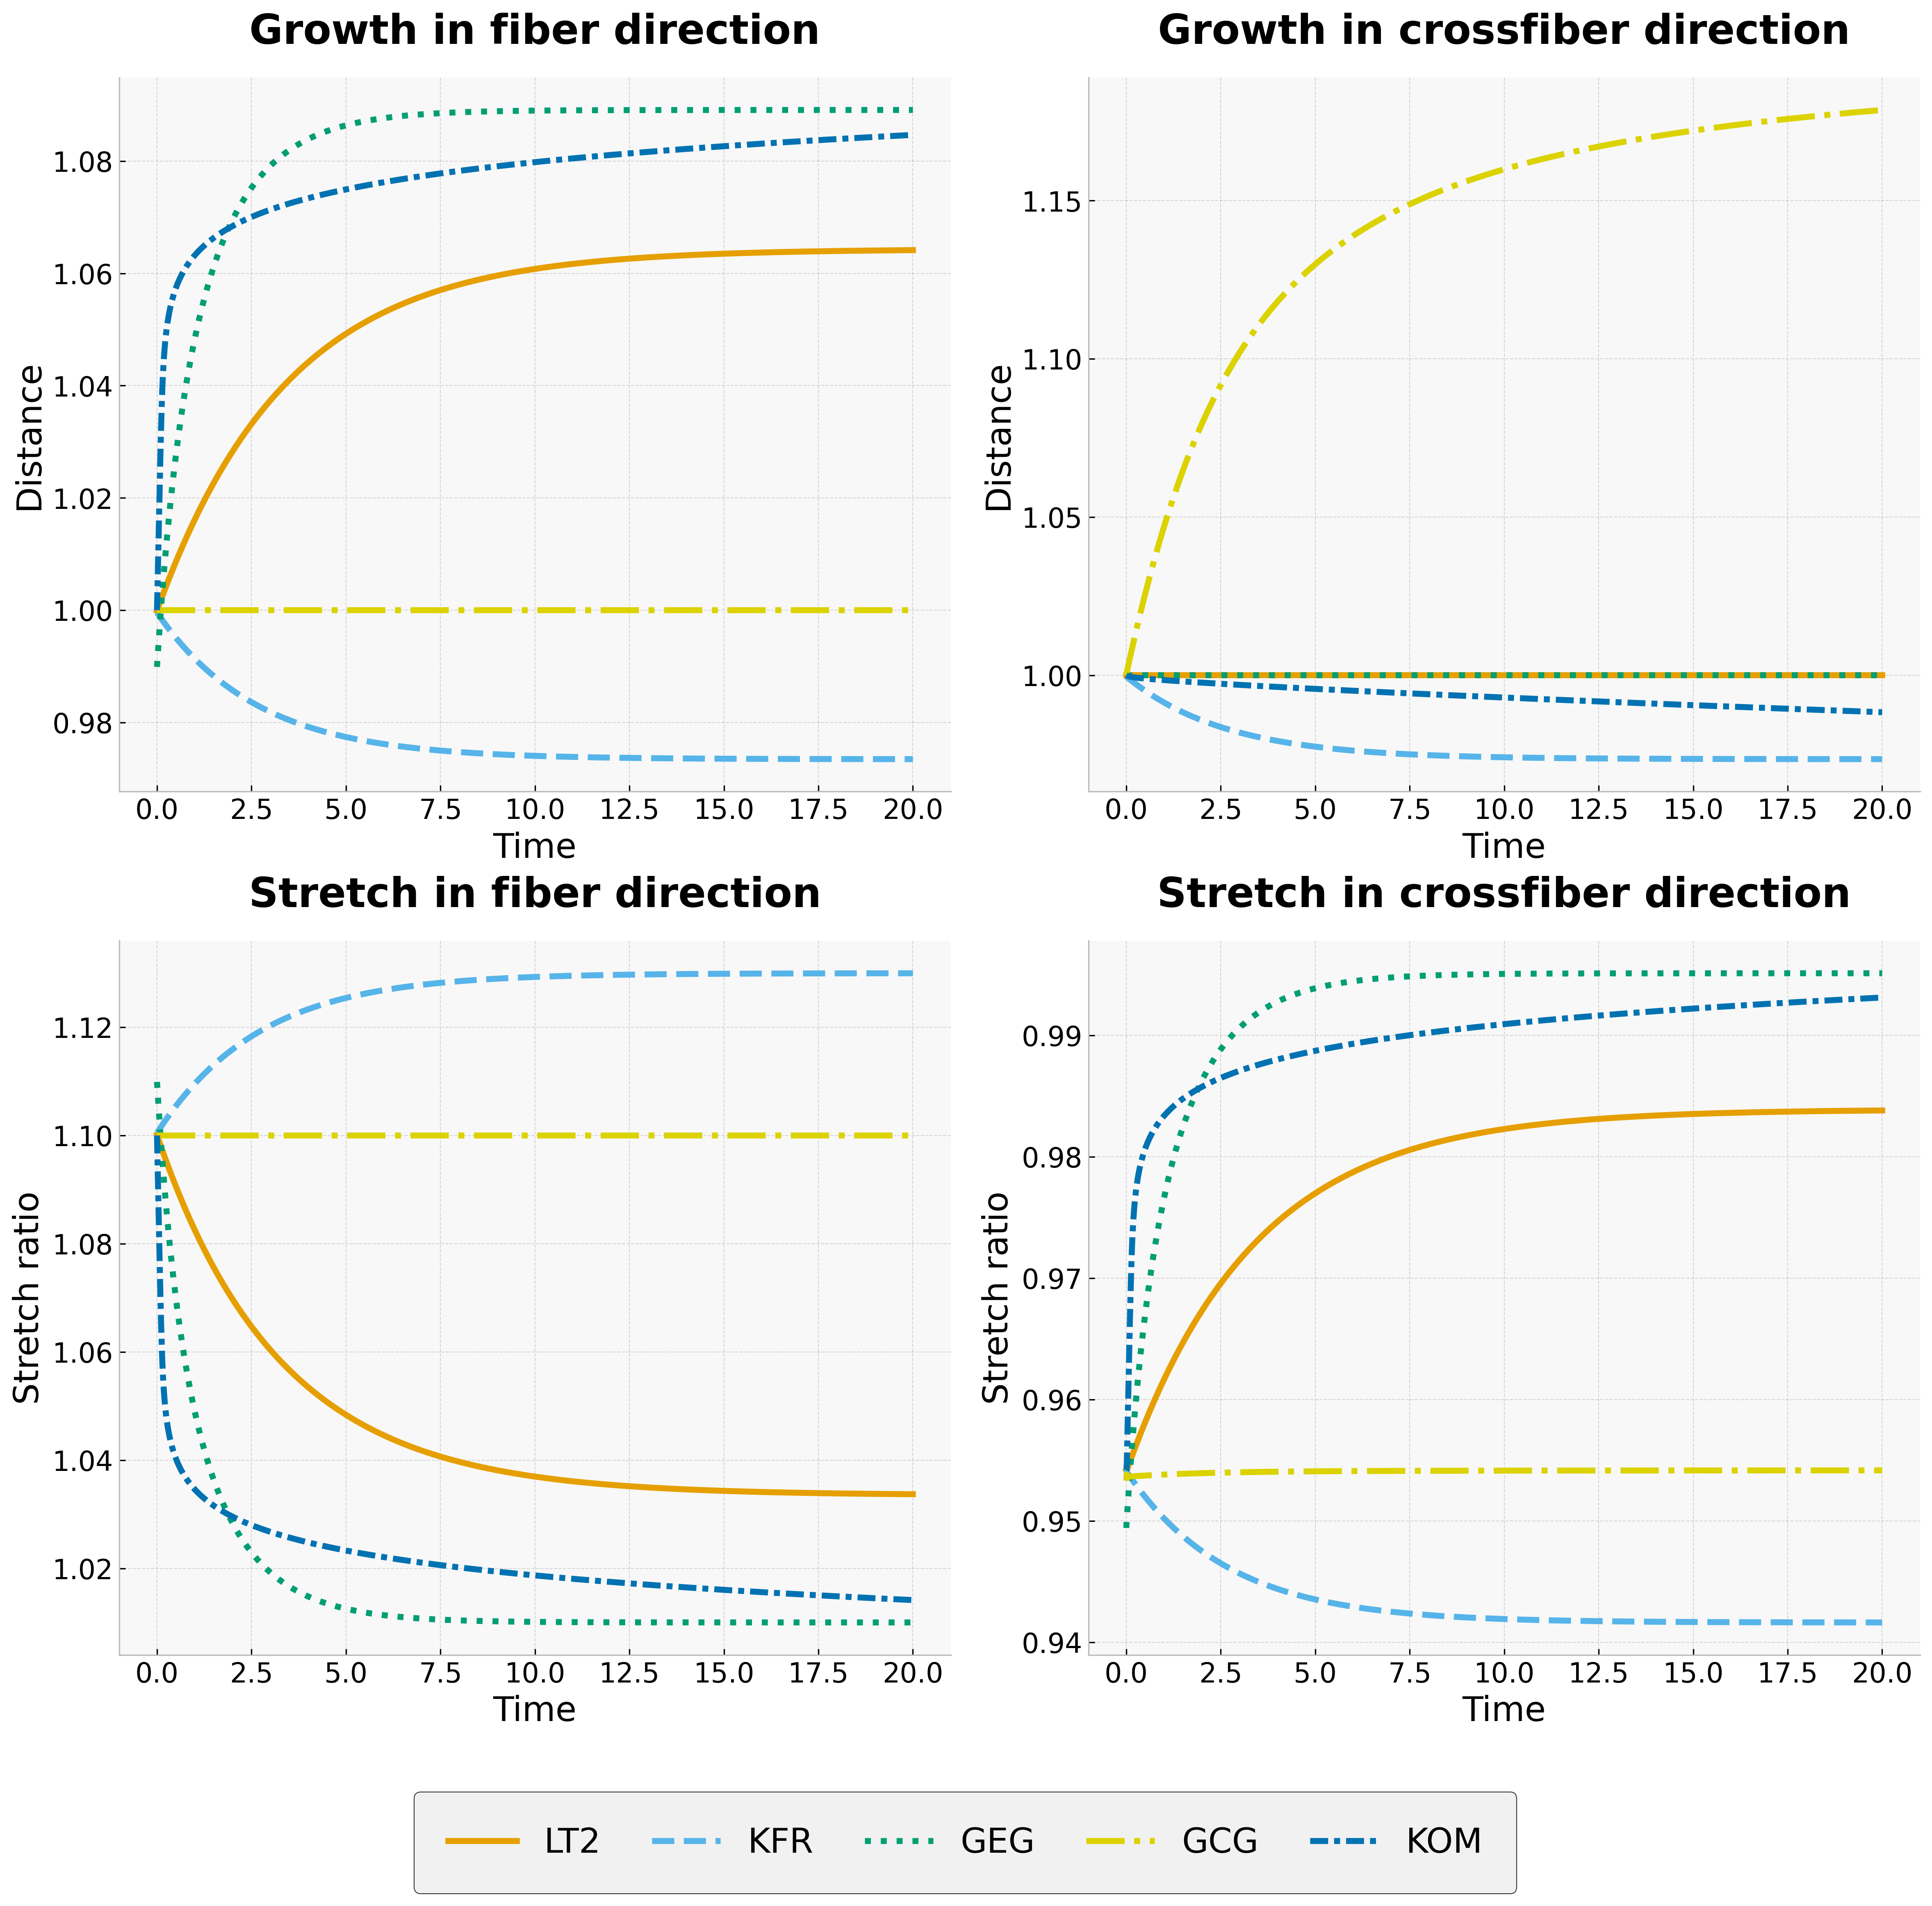
\includegraphics[width=\textwidth]{10p_stretch_3.png}
    \caption{Growth and stretch predicted by a 10\% stretch in the fiber direction.}
    \label{fig:10p_stretch}
\end{figure}
\begin{figure}[h]
    \centering
    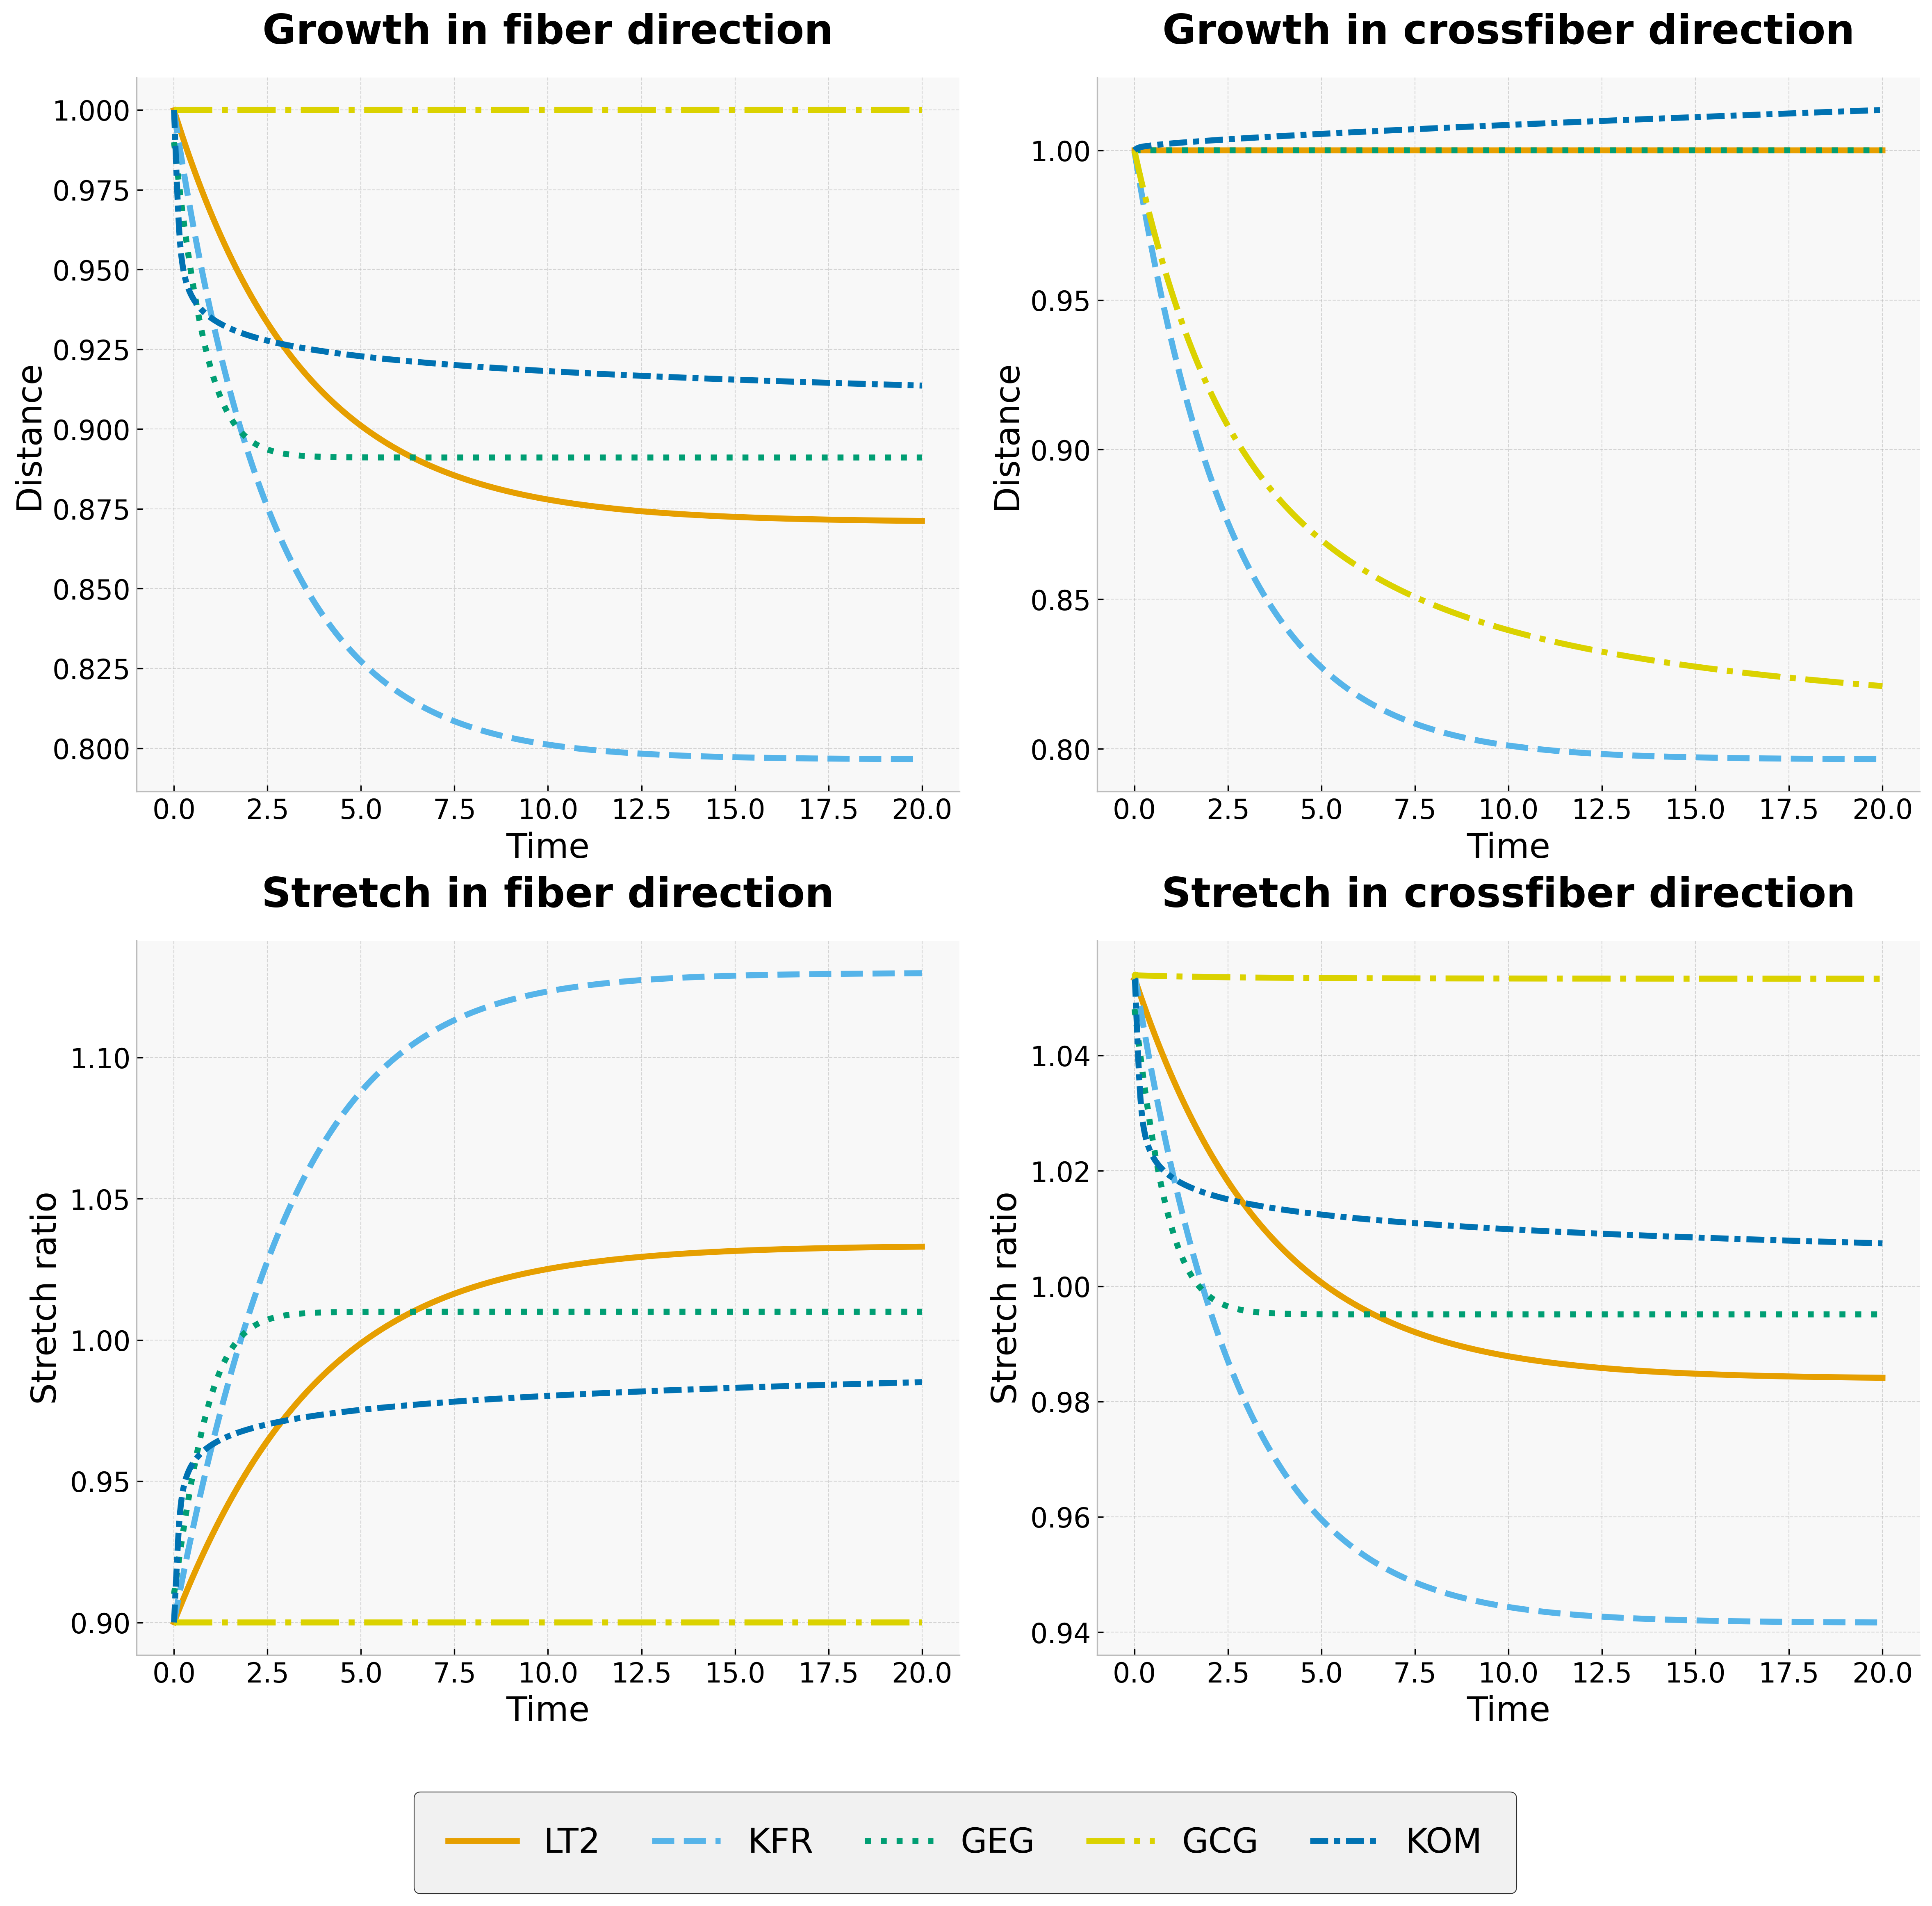
\includegraphics[width=\textwidth]{10p_compression_3.png}
    \caption{Growth and stretch predicted by a 10\% compression in the fiber direction.}
    \label{fig:10p_compression}
\end{figure}    

\section{Conclusion and future work}
We have implemented a general growth and remodelling framework using the FEniCSx program in Python. The goal is to easily change material models and growth models. This will allow researchers to compare their models with other models in the field. Future work will include implementing more complex geometries, more growth laws, and more material models. The models we have used in this paper are not derived from the dissipation equation but are instead phenomenologically derived growth laws and future work should investigate whether or not they satisfy the laws of thermodynamics. Another avenue of future research we wish to pursue is to look into constrained mixture models which model how changes in the various constituents influence the characteristics of the tissue. We also wish to add models that have more mathematically sophisticated stopping criteria, such as the ones developed by Erlich et al. \citep{Erlich2023} uses an energy penalty to construct a stopping criteria and \citep{Erlich2024} looks into how curvature\footnote{The intrinsic three dimensional curvature, not the two dimensional curvature of the surface of the body.} in the reference configuration could be used as a stopping criteria. Future work will also implement the growth models on geometries with fibers. We tried running the models on various fiber orientations and found them extremely sensitive to fibers that varied throughout the domain. Preliminary results indicate that some of the models do not converge to a steady state for relatively small perturbations of the variables or if the fibers are not well aligned with the body, something we plan on quantifying in the future. \par
When this package is further developed we aim to add it to the Pulse\footnote{https://github.com/finsberg/fenicsx-pulse} package. \par
The models we compared have been developed to capture different aspects of growth and were tuned to be used on different material models, so an apples-to-apples comparison might not be fair. Furthermore, the growth models we have used are not taking into account residual stresses that exist within the material before or after growth occurs. \par
Finally, experimental data is needed to verify which models are accurate or capture the correct phenomena of growing cardiac tissue.
% \newpage
\bibliographystyle{spbasic}
\bibliography{chapters/munthe/bibliography.bib}
% \printbibliography
% \end{document}



% Write the full path to the location of the graphics relative to book.tex
% \graphicspath{{chapters/chp1/graphics/}}

\title{Blood flow in the beating heart: Coupling fluid dynamics to reduced wall and circulation models for data-driven cardiac FSI}
\titlerunning{Blood flow in the beating heart}

\author{Marc Hirschvogel, Mia Bonini, Maximilian Balmus, David Nordsletten}
\authorrunning{Hirschvogel et al.}

\institute{Marc Hirschvogel \email{marc.hirschvogel@polimi.it} \at MOX, Dipartimento di Matematica, Politecnico di Milano, Milan, Italy}

\maketitle

\abstract{We present a fluid-reduced-solid interaction (FrSI) approach suitable for modeling blood flow in the beating left heart. 
The method uses image-derived model data to construct a suitable boundary motion space, enhanced by a reduced solid mechanics wall model to enable adaptive fluid motion. 
The method combines the efficiency of fluid dynamics models with features from full FSI approaches, uniquely integrating motion data to predict cardiac hemodynamics over a full heart cycle. 
The approach is presented for a patient-specific left heart model coupled to a lumped circulatory system, showing physiological flow behavior and pressure-volume relations.}


\section*{Introduction}
Computational fluid dynamics (CFD) provides a valuable tool to predict blood flow in the cardiovascular system \cite{schwarz2023}. 
Models of blood flow in the heart have become relevant to predict various cardiovascular conditions, where motion states from imaging are used \cite{bonini2022-suppl,zingaro2023,garciavillalba2021} or even fully-coupled fluid-solid interaction (FSI) models are employed \cite{nordsletten2011-fsi,mccormick2011modelling}. 
However, prescribed cavity motion reduces the model's ability to adapt under varying loads, and full FSI models are complex, computationally demanding, and difficult to constrain (uncertain boundary conditions and sparse patient data for reliable geometry reconstruction).
The fluid-reduced-solid interaction (FrSI) method closes the gap between model complexity and efficiency. This is a data-informed model reduction approach, particularly suited for cardiac FSI \cite{hirschvogel2024-frsi}. 
The method combines physics- with projection-based model reduction techniques that leverage Proper Orthogonal Decomposition (POD) modes derived from imaging (or some high-fidelity model) to build a reduced-order model (ROM), combined with a structural model of the ventricular wall defined on a 2D manifold.
In this contribution, we show the FrSI method's applicability to a complex, patient-specific left heart model, with a particular focus on monolithic solver implementations in FEniCSx \cite{alnaes2015fenics, baratta2023dolfinx}. This method encompasses the implementation of an Arbitrary Lagrangian-Eulerian (ALE) fluid mechanics problem subject to non-local constraints (Galerkin ROM, 3D-0D coupling to lumped circulation models). 
The solver and preconditioning aspects of this model and other fluid dynamics problems under non-local boundary conditions have been introduced in \cite{hirschvogel2025-prec}.


\section*{Methods}
The fluid-reduced-solid interaction (FrSI) problem of a 3D left heart model (atrium, ventricle, aortic outflow tract) along with the underlying data sources is depicted in Fig.~\ref{fig:heart_problem}. 
In particular, domain and motion data are retrieved from time-resolved dynamic computed tomography (CT), which are subsequently mapped to a finite element mesh in order to generate a discrete space of modes using POD \cite{rathinam2003}. 
The model is further coupled to a closed-loop systemic, pulmonary, and coronary circulation system \cite{hirschvogel2017,arthurs2016} in order to provide physiologically meaningful cardiovascular loads to the 3D model.
\begin{figure}[!htp]
\centering
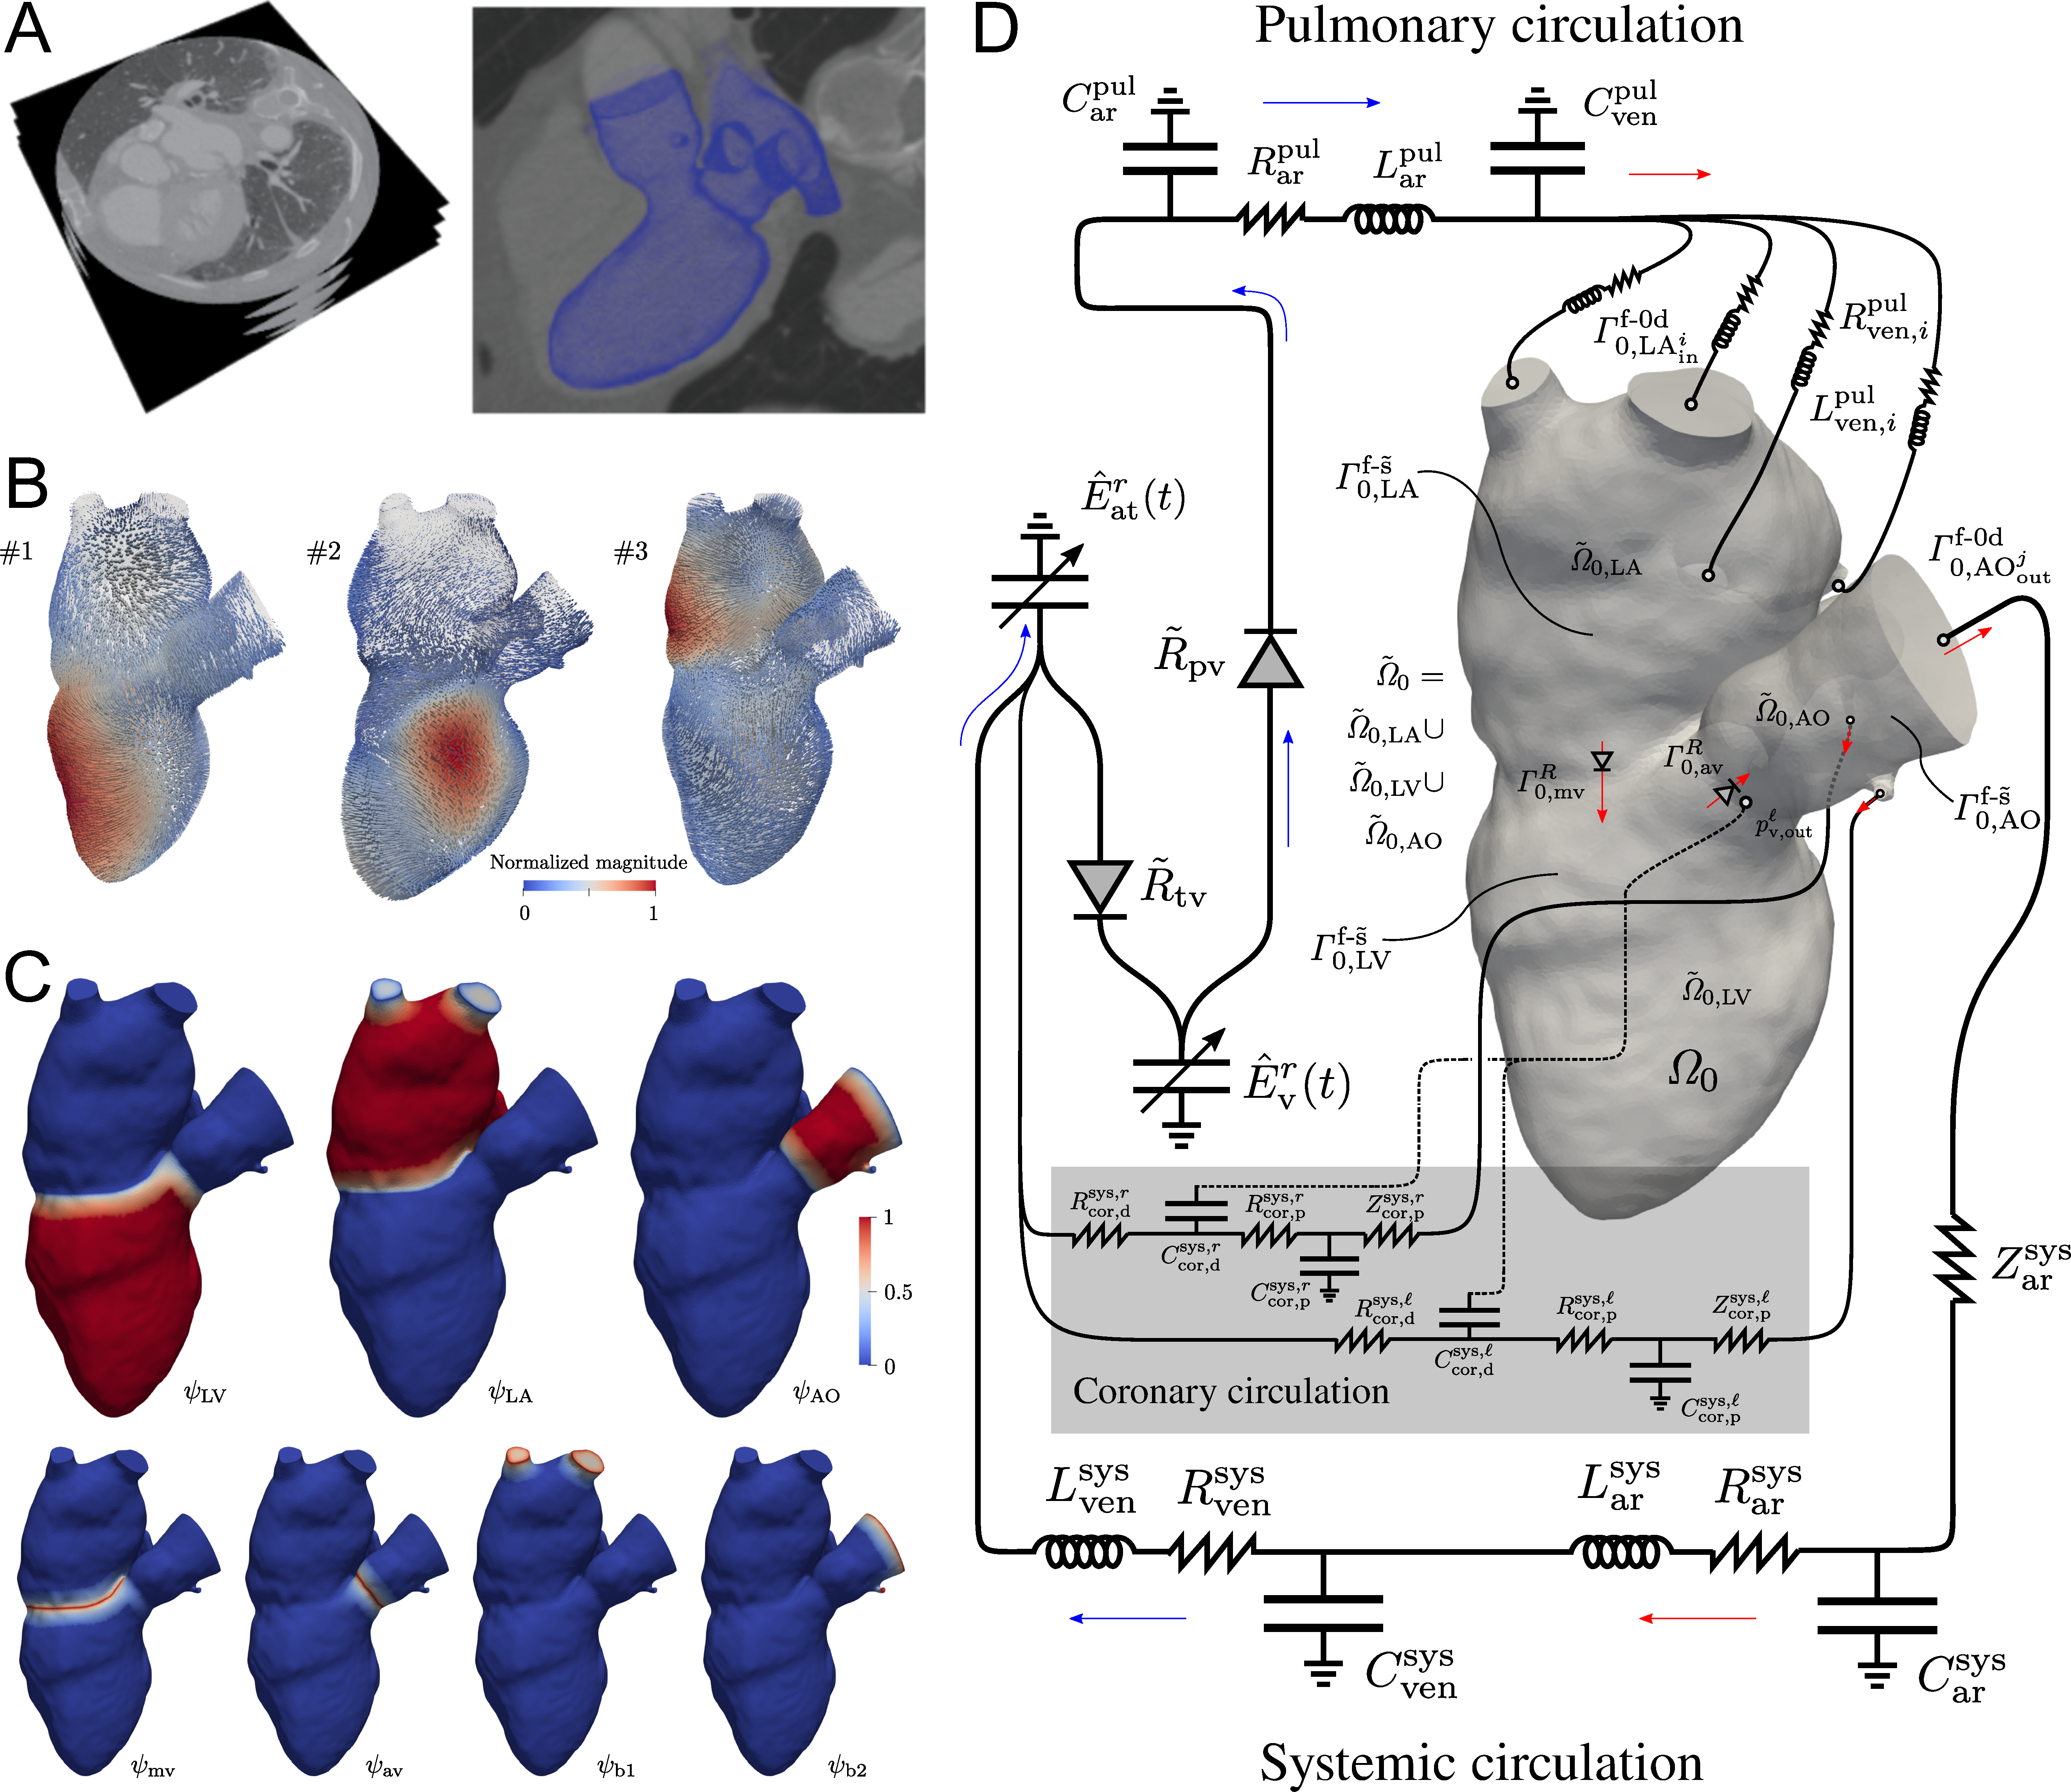
\includegraphics[width=1\textwidth]{chapters/hirschvogel/heart_problem.pdf}
\caption{\textbf{A.} Dynamic cardiac computed tomography (CT) images with contrast and dynamic segmentation of left heart lumen for subsequent finite element mesh generation, motion tracking of deformation over the heart cycle. 
\textbf{B.} Principal component analysis by means of Proper Orthogonal Decomposition (POD) of wall motion space. The first three most dominant POD modes are shown (10 are used). 
\textbf{C.} Partition of unity fields for regional decomposition of POD space: Atrium, ventricle, and aortic outflow tract---as well as their junctions and truncations around the in-/outflows---can exhibit independent kinematics. 
\textbf{D.} 3D-0D coupled FrSI model of the left heart.}\label{fig:heart_problem}
\end{figure}

\subsection*{Preprocessing of patient data}
The FrSI approach relies on external data sourced either from some high-dimensional model or from patient-specific imaging data. Here, we build a patient-specific model of the left heart by segmenting a dynamic cardiac CT data set using 3D Slicer \cite{kikinis2014-3dslicer}, cf. Fig.~\ref{fig:heart_problem}A. Subsequently, a diastolic frame is meshed with SimModeler \cite{simmodeler}, and a motion tracking algorithm is used to extract the wall velocities at each frame and map them to the finite element mesh (with velocity degree of freedom space of size $n_{v}$). Thereafter, the wall velocity data for $m=19$ frames is collected into a snapshot matrix $\hat{\boldsymbol{\mathsf{S}}} \in \mathbb{R}^{n_{v} \times m}$, and the eigenvalue problem
\begin{align}
    (\hat{\boldsymbol{\mathsf{S}}}^{\mathrm{T}} \hat{\boldsymbol{\mathsf{S}}}) \,\boldsymbol{\uppsi}_{i} = \uplambda_{i} \,\boldsymbol{\uppsi}_{i}, \quad i = 1, \hdots, m,\label{eq:rom_eigensolve}
\end{align}
is solved, with eigenvalues $\uplambda$ and eigenvectors $\boldsymbol{\uppsi} \in \mathbb{R}^{m}$. The first $r_{v}$ POD modes $\boldsymbol{\upphi} \in \mathbb{R}^{n_{v}}$ then can be computed as follows:
\begin{align}
    \boldsymbol{\upphi}_{j} = \frac{1}{\sqrt{\uplambda_{j}}} \hat{\boldsymbol{\mathsf{S}}} \boldsymbol{\uppsi}_{j}, \quad j = 1, \hdots, r_{v}, \label{eq:phi_Phi_frsi}
\end{align}
of which the first three are shown in Fig.~\ref{fig:heart_problem}B. A suitable Galerkin model reduction operator,
\begin{align}
    \boldsymbol{\mathsf{V}}_{v}^{\mathit{\Gamma}} \in \mathbb{R}^{n_v \times (r_v + n_{v}^{\mathit{\Omega}})}, \label{eq:Vgamma}
\end{align}
then needs to be defined, with $n_{v}^{\mathit{\Omega}}$ as the size of the space of bulk (non-boundary) velocities. In Eq.~(\ref{eq:Vgamma}), POD modes Eq.~(\ref{eq:phi_Phi_frsi}) have to be incorporated such that velocity degrees of freedom on $\mathit{\Gamma}_{0}^{\mathrm{f}\text{-}\tilde{\mathrm{s}}}$ are confined to the lower-dimensional subspace, but those associated to the bulk domain remain unconstrained \cite{hirschvogel2024-frsi}. Furthermore, the POD space is decomposed with a partition of unity approach such that each region can exhibit independent kinematics, cf. Fig.~\ref{fig:heart_problem}C.

\subsection*{Strong form problem statement}
Here, we briefly state the strong problem of FrSI---fluid dynamics in an ALE reference frame \cite{donea1982,duarte2004} with a reduced structural wall model---subject to non-local flux-dependent tractions at the in- and outflows. The boundary subspace projection is then performed on the discrete system presented in a later section.\\

The incompressible non-conservative ALE Navier-Stokes equations, defining the conservation of linear momentum and mass over the domain $\mathit{\mathit{\Omega}}$ is written as:
\begin{align}
	\rho\left(\left.\frac{\partial \boldsymbol{v}}{\partial t}\right|_{\boldsymbol{x}_{0}} + \nabla\boldsymbol{v} (\boldsymbol{v}-\boldsymbol{w})\right) &= \nabla\cdot\boldsymbol{\sigma} && \;\text{in}\; \mathit{\mathit{\Omega}} \times [0,T], \label{eq:ns_strong_mom}\\
	\nabla\cdot\boldsymbol{v} &= 0 && \;\text{in}\; \mathit{\mathit{\Omega}} \times [0,T], \label{eq:ns_strong_mass}
\end{align}
where $\nabla$ is the gradient operator with respect to physical space ($\nabla\boldsymbol{v}:=\frac{\partial v_{i}}{\partial x_{j}}\boldsymbol{e}_{i}\otimes\boldsymbol{e}_{j}$) and $\left.\frac{\partial (\bullet)}{\partial t}\right|_{\boldsymbol{x}_{0}}$ the time derivative in the ALE frame. Further, $\boldsymbol{v}$ and $p$ are the fluid's velocity and pressure, $\boldsymbol{w}$ is the ALE domain velocity, and $\rho=1.025\cdot 10^{-6}\;\frac{\mathrm{kg}}{\mathrm{mm}^{3}}$ the blood density. 
The ventricular blood is assumed to be a Newtonian fluid, making the Cauchy stress $\boldsymbol{\sigma} = -p \boldsymbol{I} + \mu \left(\nabla \boldsymbol{v} + (\nabla \boldsymbol{v})^{\mathrm{T}}\right)$, with the dynamic viscosity $\mu=4\cdot 10^{-6}\;\mathrm{kPa\cdot s}$. 
The fluid's boundary wall $\mathit{\Gamma}_{0}^{\mathrm{f}\text{-}\tilde{\mathrm{s}}}$ is assumed deformable and is described by a reduced solid mechanics model governed by the balance of linear momentum of finite strain elastodynamics, which entails the physics component of the FrSI method \cite{hirschvogel2024-frsi}. 
Since the displacement field at the boundary can be entirely derived from the fluid's velocity field, kinematic compatibility and continuity of tractions are readily fulfilled by incorporating the following boundary traction, cf. comparable derivations for small strain solid wall models \cite{colciago2014}:
\begin{align}
    \boldsymbol{t}_{0}^{\mathrm{f}\text{-}\tilde{\mathrm{s}}} &= -h_0\left(\rho_{0,\mathrm{s}} \frac{\partial \boldsymbol{v}}{\partial t} - \tilde{\nabla}_{0}\cdot\tilde{\boldsymbol{P}}\right) \quad &&\text{on} \; \mathit{\Gamma}_{0}^{\mathrm{f}\text{-}\tilde{\mathrm{s}}} \times [0,T], \label{eq:frsi_tsolid_gen}
\end{align}
where $\tilde{\nabla}_{0}$ is a Nabla operator with respect to the reference frame (considering only in-plane derivatives), $h_0$ a wall thickness parameter (here $10\;\mathrm{mm}$ for ventricle, $5\;\mathrm{mm}$ for atrium, and $1\;\mathrm{mm}$ for aortic arch), $\rho_{0,\mathrm{s}}=10^{-6}\;\frac{\mathrm{kg}}{\mathrm{mm}^{3}}$ the reduced solid's density, and $\tilde{\boldsymbol{P}}=\tilde{\boldsymbol{P}}(\boldsymbol{u}_{\mathrm{f}}(\boldsymbol{v}) + \boldsymbol{u}_{\mathrm{pre}}, \boldsymbol{v})$ the first Piola-Kirchhoff stress---a general function of the fluid velocity and the fluid displacement at the boundary:
\begin{align}
    \boldsymbol{u}_{\mathrm{f}}(\boldsymbol{v}) = \int\limits_{0}^{t}\boldsymbol{v}\,\mathrm{d}\bar{t}
    \label{eq:ufluid}.
\end{align}
The first Piola-Kirchhoff stress is mapped from its material counterpart, the second Piola-Kirchhoff stress, $\tilde{\boldsymbol{P}} = (\boldsymbol{F}_{\mathrm{f}} - \boldsymbol{F}_{\mathrm{f}}\,\boldsymbol{n}_{0}\otimes\boldsymbol{n}_{0}) \tilde{\boldsymbol{S}}$, with the fluid deformation gradient $\boldsymbol{F}_{\mathrm{f}} = \boldsymbol{I} + \nabla_{0}\boldsymbol{u}_{\mathrm{f}}$, using Eq.~(\ref{eq:ufluid}). By eliminating its normal components and re-defining the out-of-plane stretch on assumptions of incompressibility, a membrane right Cauchy-Green tensor, $\tilde{\boldsymbol{C}}$, for the surface as well as its time derivative can be defined. Finally, $\boldsymbol{u}_{\mathrm{pre}}$ is a prestress displacement computed by methods described in \cite{schein2021,gee2010}. More details on the kinematics and prestress for FrSI can be found in \cite{hirschvogel2024-frsi}. The constitutive equation for the reduced solid second Piola-Kirchhoff stress is
\begin{align}
\tilde{\boldsymbol{S}} = 2\frac{\partial\mathit{\Psi}(\tilde{\boldsymbol{C}})}{\partial \tilde{\boldsymbol{C}}} + 2\frac{\partial\mathit{\Psi}_{\mathrm{v}}(\dot{\tilde{\boldsymbol{C}}})}{\partial \dot{\tilde{\boldsymbol{C}}}} + \tau_{\mathrm{a}}(t) \boldsymbol{A}_{0}, \label{eq:S_red}
\end{align}
with a structural tensor $\boldsymbol{A}_{0}=\boldsymbol{I}$ for the atrium (isotropic active stress), $\boldsymbol{A}_{0}=\tilde{\boldsymbol{M}}_{0}$ for the ventricle (active stress in directions of a reduced structural tensor \cite{hirschvogel2024-frsi}), or $\boldsymbol{A}_{0}=\boldsymbol{0}$ for the aortic arch (no active stress). The active stress $\tau_{\mathrm{a}}(t)$ follows the solution of an evolution equation, cf. \cite{hirschvogel2017}. The passive elastic model is of isotropic-exponential type\footnote{While the myocardium typically exhibits highly anisotropic passive properties \cite{holzapfel2009}, it remains inconclusive how its transmurally varying fiber, sheet, and sheet-normal architecture---governing its anisotropic stiffness---can be consistently homogenized throughout the wall and mapped to a 2D surface representation. Since our focus primarily addresses adaptive fluid motion, we prefer an isotropic 2D model whose parameters easily can be calibrated to observed (diastolic) pressure-volume data.} \cite{demiray1972}, and a typical viscous pseudo-potential is used \cite{chapelle2012}.\\

The coupling to the circulatory system is expressed via $n_{\mathrm{0d}}^{\mathrm{b}}=7$ non-local constraints, enforcing consistency between the flux over the 3D-0D boundary $\mathit{\Gamma}_{i}^{\mathrm{f}\text{-}\mathrm{0d}}$ and the flux variable $q_{i}^{\mathrm{0d}}$ from the 0D model:
\begin{align}
    \int\limits_{\mathit{\Gamma}_{i}^{\mathrm{f}\text{-}\mathrm{0d}}} (\boldsymbol{v}-\widehat{\boldsymbol{w}})\cdot\boldsymbol{n}\,\mathrm{d}A &= \alpha_{i} q_{i}^{\mathrm{0d}}(\{\mathit{\Lambda}\}_{n_{\mathrm{0d}}^{\mathrm{b}}}) \quad &&\text{in} \; [0,T]. \label{eq:3d0d_constraint}
\end{align}
Therein, $\boldsymbol{n}$ is a unit outward normal of the current frame, and scaling parameters, $\alpha_i$, account for the directionality of flow, i.e. should take the value of $-1$ if a 0D flux variable is imposed as an inflow to the fluid domain, and $1$ otherwise. The multipliers $\{\mathit{\Lambda}\}_{n_{\mathrm{0d}}^{\mathrm{b}}}$ impose normal tractions (pressure loads) on their respective in-/outflow boundaries:
\begin{align}
    \boldsymbol{t}_{i}^{\mathrm{\mathrm{f}\text{-}\mathrm{0d}}} &= -\mathit{\Lambda}_{i} \,\boldsymbol{n} \quad &&\text{on} \; \mathit{\Gamma}_{i}^{\mathrm{f}\text{-}\mathrm{0d}} \times [0,T]. \label{eq:frsi_t0d_gen}
\end{align}
The deformability of the fluid domain here is described by a pseudo-solid's displacement field $\boldsymbol{d}$ governed by 
\begin{align}
    \nabla_{0}\cdot \boldsymbol{\sigma}_{\mathrm{g}} &= \boldsymbol{0} \quad &&\text{in} \;\mathit{\Omega}_{0} \times [0,T], \label{eq:ale_strong_gen}\\
    \boldsymbol{d} &= \boldsymbol{u}_{\mathrm{f}}(\boldsymbol{v}) 
    \quad &&  
    \text{on}\; \mathit{\Gamma}_{0}^{\mathrm{f}\text{-}\tilde{\mathrm{s}}} \times [0,T], \label{eq:ale_dbc_gen}
\end{align}
subject to the essential boundary condition on $\mathit{\Gamma}_{0}^{\mathrm{f}\text{-}\tilde{\mathrm{s}}}$, requiring $\boldsymbol{d}$ to take the value of the fluid displacement Eq.~(\ref{eq:ufluid}). Here, we use a fully nonlinear ALE model of coupled Neo-Hookean type \cite{holzapfel2000}, which, on the discrete space, is scaled by the inverse of the reference cell's Jacobian determinant \cite{shamanskiy2021}. This scaling allows allocating stiffness to more anisotropic boundary elements and have the more regularly shaped bulk elements bear most of the deformation. The ALE deformation gradient and its determinant---as well as the grid/ALE convective velocity in Eq.~(\ref{eq:ns_strong_mom})---are given by
\begin{align}
    \widehat{\boldsymbol{F}}=\boldsymbol{I}+\nabla_{0}\boldsymbol{d}, \quad \widehat{J}=\det\widehat{\boldsymbol{F}}, \quad \text{and} \quad \widehat{\boldsymbol{w}}=\frac{\partial\boldsymbol{d}}{\partial t}.
    \label{eq:defgrad_ale}
\end{align}


\subsection*{Weak form and linearization}
In the following, we define the continuous weak forms of the strong problem statements suitable for a monolithic finite element implementation in FEniCSx. 
For this purpose, all integrals are formulated over the respective reference domains, and all gradient operators relate to the undeformed configuration $\mathit{\Omega}_{0}$. 
The general weak problem can be stated as follows:\\

Find fluid velocity $\boldsymbol{v}$, pressure $p$, multiplier variables $\{\mathit{\Lambda}\}_{n_{\mathrm{0d}}^{\mathrm{b}}}$, and ALE domain displacements $\boldsymbol{d}$ such that conservation of linear momentum,
\begin{equation}
\begin{aligned}
    &R_{\delta v}\left(\boldsymbol{v},p,\{\mathit{\Lambda}\}_{n_{\mathrm{0d}}^{\mathrm{b}}},\boldsymbol{d};\delta\boldsymbol{v}\right) := \int\limits_{\mathit{\Omega}_0} \widehat{J} \rho  \left(\left.\frac{\partial\boldsymbol{v}}{\partial t}\right|_{\boldsymbol{x}_{0}} + \left(\nabla_{0}\boldsymbol{v}\,\widehat{\boldsymbol{F}}^{-1}\right)\,\left(\boldsymbol{v}-\widehat{\boldsymbol{w}}\right)\right) \cdot \delta\boldsymbol{v} \,\mathrm{d}V_0 \\ &
    + \int\limits_{\mathit{\Omega}_0} \widehat{J}\,\boldsymbol{\sigma}(\boldsymbol{v},p,\boldsymbol{d}) : \nabla_{0} \delta\boldsymbol{v}\,\widehat{\boldsymbol{F}}^{-1} \,\mathrm{d}V_0 + \sum\limits_{i=1}^{n_{\mathrm{0d}}^{\mathrm{b}}} \mathit{\Lambda}_{i} \int\limits_{\mathit{\Gamma}_{0,i}^{\mathrm{f}\text{-}\mathrm{0d}}} \widehat{J}\widehat{\boldsymbol{F}}^{-\mathrm{T}}\boldsymbol{n}_{0}\cdot\delta\boldsymbol{v}\,\mathrm{d}A_0 \\
    &+ \int\limits_{\mathit{\Gamma}_{0}^{\mathrm{f}\text{-}\tilde{\mathrm{s}}}} h_0 \left(\rho_{0,\mathrm{s}}\,\frac{\partial\boldsymbol{v}}{\partial t} \cdot \delta\boldsymbol{v} + \tilde{\boldsymbol{P}}\left(\boldsymbol{u}_{\mathrm{f}}(\boldsymbol{v}) + \boldsymbol{u}_{\mathrm{pre}},\boldsymbol{v}\right) : \tilde{\nabla}_{0} \delta\boldsymbol{v}\right) \,\mathrm{d}A_0 \\
    &+ R_{\delta v}^{R}(\boldsymbol{v},\boldsymbol{d};\delta\boldsymbol{v}) + S_{\delta v}^{\mathrm{D}}(\boldsymbol{v},p,\boldsymbol{d};\delta\boldsymbol{v}) + S_{\delta v}^{\mathrm{out}}(\boldsymbol{v},\boldsymbol{d};\delta\boldsymbol{v}) = 0, \label{eq:frsi_weakform_v}
\end{aligned}
\end{equation}
conservation of mass,
\begin{align}
    R_{\delta p}(\boldsymbol{v},\boldsymbol{d};\delta p) := 
    \int\limits_{\tilde{\mathit{\Omega}}_0} \widehat{J}\,\nabla_{0}\boldsymbol{v} : \widehat{\boldsymbol{F}}^{-\mathrm{T}}\delta p\,\mathrm{d}V_0 + S_{\delta p}^{\mathrm{D}}(\boldsymbol{v},p,\boldsymbol{d};\delta p) = 0,\label{eq:frsi_weakform_p}
\end{align}
constraints enforcing consistency between 0D and 3D models,
\begin{equation}
\begin{aligned}
    &R_{\delta\mathit{\Lambda}} \left(\boldsymbol{v}, \{\mathit{\Lambda}\}_{n_{\mathrm{0d}}^{\mathrm{b}}}, \boldsymbol{d}; \{\delta\mathit{\Lambda}\}_{n_{\mathrm{0d}}^{\mathrm{b}}}\right) := \\
    &\sum\limits_{i=1}^{n_{\mathrm{0d}}^{\mathrm{b}}} \left(\,\int\limits_{\mathit{\Gamma}_{0,i}^{\mathrm{f}\text{-}\mathrm{0d}}} (\boldsymbol{v}-\widehat{\boldsymbol{w}})\cdot\widehat{J}\widehat{\boldsymbol{F}}^{-\mathrm{T}}\boldsymbol{n}_{0}\,\mathrm{d}A_0 - \alpha_i\,q_{i}^{\mathrm{0d}}\left(\{\mathit{\Lambda}\}_{n_{\mathrm{0d}}^{\mathrm{b}}}\right)\right)\delta\mathit{\Lambda}_{i} = 0,
    \label{eq:frsi_3d0d_coupling_weakform}
\end{aligned}
\end{equation}
as well as ALE domain motion,
\begin{align}
    R_{\delta d}(\boldsymbol{d},\boldsymbol{v};\delta\boldsymbol{d}) &:= \int\limits_{\mathit{\Omega}_0}\boldsymbol{\sigma}_{\mathrm{g}}(\boldsymbol{d}) : \nabla_{0}\delta\boldsymbol{d}\,\mathrm{d}V_0 = 0,\label{eq:ale_weakform}
\end{align}
hold true, for all fluid velocity and pressure test functions $\left(\delta\boldsymbol{v},\, \delta p\right)$, ALE domain motion test functions ($\delta\boldsymbol{d}$), as well as multiplier test functions ($\{\delta\mathit{\Lambda}\}_{n_{\mathrm{0d}}^{\mathrm{b}}}$). The ALE problem is further subject to the essential boundary condition Eq.~(\ref{eq:ale_dbc_gen}) at the deformable interface where the reduced solid is defined. The constitutive equation for the Cauchy stress is written with respect to the reference frame, $\boldsymbol{\sigma}(\boldsymbol{v},p,\boldsymbol{d}) = -p \boldsymbol{I} + \mu \left(\nabla_0 \boldsymbol{v}\,\widehat{\boldsymbol{F}}^{-1} + \widehat{\boldsymbol{F}}^{-\mathrm{T}}(\nabla_0 \boldsymbol{v})^{\mathrm{T}}\right)$. In Eq.~(\ref{eq:frsi_weakform_v}), $R_{\delta v}^{R}(\boldsymbol{v},\boldsymbol{d};\delta\boldsymbol{v})$ is a Robin term used to impose pressure jump-dependent tractions at the mitral and aortic valve planes.
This represents a particular challenge, since effects of the mitral and aortic valves need pressure discontinuities across the interfaces of atrium and ventricle as well as ventricle and aortic root. For this purpose, very recently introduced \textit{mixed-dimensional} functionality of FEniCSx is leveraged. This allows to create sub-discretizations (of equal or lower dimension) and make use of functions defined on different but related meshes within one finite element form. Here, the function space for the fluid pressure is defined on each sub-mesh (atrium, ventricle, aorta), and hence is allowed to jump across their respective interfaces. More details on the valve models can be found in \cite{hirschvogel2025-prec}.
Furthermore, the terms $S_{\delta v}^{\mathrm{D}}(\boldsymbol{v},p,\boldsymbol{d};\delta\boldsymbol{v})$ in Eq.~(\ref{eq:frsi_weakform_v}) and $S_{\delta p}^{\mathrm{D}}(\boldsymbol{v},p,\boldsymbol{d};\delta p)$ in Eq.~(\ref{eq:frsi_weakform_p}) refer to stabilization operators suitable for first-order approximations of both fluid velocity and pressure. Here, we make use of a variant of the G2 stabilization method \cite{johnson1998,hoffman2003,hessenthaler2017}. Furthermore, to prevent backflow-induced divergence, all Neumann/3D-0D coupling boundaries are subject to an outflow stabilization \cite{esmailymoghadam2011}, referred to by the term $S_{\delta v}^{\mathrm{out}}(\boldsymbol{v},\boldsymbol{d};\delta\boldsymbol{v})$ in Eq.~(\ref{eq:frsi_weakform_v}).

Flux variables $q_{j}^{\mathrm{0d}} = \boldsymbol{\mathsf{y}}\cdot\boldsymbol{\mathsf{e}}_{j}$ in Eq.~(\ref{eq:frsi_3d0d_coupling_weakform}) are, in general, solutions to a set of $n_{\mathrm{0d}}^{\mathrm{e}}$ 0D algebraic and first-order ordinary differential equations in time, with the vector of state variables $\boldsymbol{\mathsf{y}}$ and $\boldsymbol{\mathsf{e}}_{j}$ as the $j$-th $n_{\mathrm{0d}}^{\mathrm{e}}$-dimensional unit vector. We may state the 0D problem as follows: Find 0D model variables $\boldsymbol{\mathsf{y}}$ such that
\begin{equation}
\begin{aligned}
    R_{\mathrm{0d}} \left(\boldsymbol{\mathsf{y}},\{\mathit{\Lambda}\}_{n_{\mathrm{0d}}^{\mathrm{b}}}; \delta\boldsymbol{\mathsf{y}}\right) :=
    \left(\dot{\boldsymbol{\mathsf{g}}}(\boldsymbol{\mathsf{y}},\{\mathit{\Lambda}\}_{n_{\mathrm{0d}}^{\mathrm{b}}}) + 
    \boldsymbol{\mathsf{f}}(\boldsymbol{\mathsf{y}},\{\mathit{\Lambda}\}_{n_{\mathrm{0d}}^{\mathrm{b}}})\right) \cdot \delta\boldsymbol{\mathsf{y}} = 0,
    \label{eq:0d_weakform}
\end{aligned}
\end{equation}
for all $\delta\boldsymbol{\mathsf{y}}$, where $\boldsymbol{\mathsf{g}}$ is a linear (``left-hand side'') and $\boldsymbol{\mathsf{f}}$ a possibly nonlinear (``right-hand side'') function in the variable vector $\boldsymbol{\mathsf{y}}$ and/or multipliers $\{\mathit{\Lambda}\}_{n_{\mathrm{0d}}^{\mathrm{b}}}$.\\

The linearizations of the weak forms Eq.~(\ref{eq:frsi_weakform_v})---(\ref{eq:ale_weakform}), being the derivatives in the direction of the velocity, pressure, multiplier, and domain displacement trial functions $\Delta\boldsymbol{v}$, $\Delta p$, $\{\Delta\mathit{\Lambda}\}_{n_{\mathrm{0d}}^{\mathrm{b}}}$, and $\Delta\boldsymbol{d}$, respectively, 
\begin{align}
    K_{\delta (\cdot)_{i} \Delta (\cdot)_{j}} := D_{\Delta (\bullet)_{j}} \left[R_{\delta (\cdot)_{i}}\right], \label{eq:linearizations}
\end{align}
are computed using symbolic automatic differentiation in FEniCSx, where $D_{\Delta (\bullet)_{j}}$ is the G{\^a}teaux operator with respect to the trial function $\Delta (\bullet)_{j}$. Due to the Dirichlet conditions on the ALE problem, a special consideration is needed for the derivative of the ALE residual with respect to the fluid velocity. Due to the nature of how Dirichlet conditions are applied in FEniCSx, this is taken care of post-discretization.

\subsection*{Discretization and solution}
The problem is discretized with finite elements of piecewise linear Lagrange polynomials in space and a single-step implicit finite difference scheme in time (One-step-$\theta$ scheme, with $\theta\in\;]0; 1]$).
The projection-based component of the FrSI method requires the reduced solid boundary to be projected to a lower-dimensional subspace spanned by POD modes, cf. Fig.~\ref{fig:heart_problem}B depicting the first three modes of this space. This is done by the boundary Galerkin projection operator Eq.~(\ref{eq:Vgamma}).
At the discrete assembled stage, at the current time-step indexed by $n+1$, we seek to find the discrete velocity $\boldsymbol{\mathsf{v}}_{n+1}$, pressure $\boldsymbol{\mathsf{p}}_{n+1}$, 3D-0D coupling multipliers $\boldsymbol{\mathsf{\Lambda}}_{n+1}$, and domain displacements $\boldsymbol{\mathsf{d}}_{n+1}$ satisfying
\begin{align}
    \boldsymbol{\mathsf{r}}_{n+1} = \begin{bmatrix} 
                  \boldsymbol{\mathsf{V}}_{v}^{\mathit{\Gamma}^\mathrm{T}}\boldsymbol{\mathsf{r}}_{v}(\boldsymbol{\mathsf{V}}_{v}^{\mathit{\Gamma}}\tilde{\boldsymbol{\mathsf{v}}},\boldsymbol{\mathsf{p}},\boldsymbol{\mathsf{\Lambda}},\boldsymbol{\mathsf{d}}) \\
                  \boldsymbol{\mathsf{r}}_{p}(\boldsymbol{\mathsf{p}},\boldsymbol{\mathsf{V}}_{v}^{\mathit{\Gamma}}\tilde{\boldsymbol{\mathsf{v}}},\boldsymbol{\mathsf{d}}) \\ 
                  \boldsymbol{\mathsf{r}}_{\mathit{\Lambda}} (\boldsymbol{\mathsf{\Lambda}},\boldsymbol{\mathsf{V}}_{v}^{\mathit{\Gamma}}\tilde{\boldsymbol{\mathsf{v}}},\boldsymbol{\mathsf{d}}) \\ 
                  \boldsymbol{\mathsf{r}}_{d} (\boldsymbol{\mathsf{d}},\boldsymbol{\mathsf{V}}_{v}^{\mathit{\Gamma}}\tilde{\boldsymbol{\mathsf{v}}})
               \end{bmatrix}_{n+1}
               = 
               \boldsymbol{\mathsf{0}},
               \label{eq:res_nonlin_frsi}
\end{align}
where $\boldsymbol{\mathsf{r}}_{v}$, $\boldsymbol{\mathsf{r}}_{p}$, $\boldsymbol{\mathsf{r}}_{\mathit{\Lambda}}$, and $\boldsymbol{\mathsf{r}}_{d}$ are the assembled discrete counterparts of Eq.~(\ref{eq:frsi_weakform_v})--(\ref{eq:ale_weakform}), respectively. 
The trial space projection is $\boldsymbol{\mathsf{v}} = \boldsymbol{\mathsf{V}}_{v}^{\mathit{\Gamma}} \tilde{\boldsymbol{\mathsf{v}}}$, where $\tilde{\boldsymbol{\mathsf{v}}}$ is the (partly) reduced-dimensional velocity vector.
In order to solve Eq.~(\ref{eq:res_nonlin_frsi}), a monolithic Newton scheme is employed, resulting in the linearized system of equations to solve for the variable increments in each nonlinear iteration indexed by $k+1$:
\begin{align}
    \begin{bmatrix} \boldsymbol{\mathsf{V}}_{v}^{\mathit{\Gamma}^\mathrm{T}}\boldsymbol{\mathsf{K}}_{vv}\boldsymbol{\mathsf{V}}_{v}^{\mathit{\Gamma}} & \boldsymbol{\mathsf{V}}_{v}^{\mathit{\Gamma}^\mathrm{T}}\boldsymbol{\mathsf{K}}_{vp} & \boldsymbol{\mathsf{V}}_{v}^{\mathit{\Gamma}^\mathrm{T}}\boldsymbol{\mathsf{K}}_{v\mathit{\Lambda}} & \boldsymbol{\mathsf{V}}_{v}^{\mathit{\Gamma}^\mathrm{T}}\boldsymbol{\mathsf{K}}_{vd} \\ \\ \boldsymbol{\mathsf{K}}_{pv}\boldsymbol{\mathsf{V}}_{v}^{\mathit{\Gamma}} & \boldsymbol{\mathsf{K}}_{pp} & \textcolor{lightgray}{\boldsymbol{\mathsf{0}}} & \boldsymbol{\mathsf{K}}_{pd} \\ \\  \boldsymbol{\mathsf{K}}_{\mathit{\Lambda} v}\boldsymbol{\mathsf{V}}_{v}^{\mathit{\Gamma}} & \textcolor{lightgray}{\boldsymbol{\mathsf{0}}} & \boldsymbol{\mathsf{K}}_{\mathit{\Lambda}\mathit{\Lambda}} & \boldsymbol{\mathsf{K}}_{\mathit{\Lambda} d} \\ \\ \boldsymbol{\mathsf{K}}_{dv}\boldsymbol{\mathsf{V}}_{v}^{\mathit{\Gamma}} & \textcolor{lightgray}{\boldsymbol{\mathsf{0}}} & \textcolor{lightgray}{\boldsymbol{\mathsf{0}}} & \boldsymbol{\mathsf{K}}_{dd} \end{bmatrix}_{n+1}^{k}\begin{bmatrix} \Delta\tilde{\boldsymbol{\mathsf{v}}} \\ \\ \Delta\boldsymbol{\mathsf{p}} \\ \\ \Delta\boldsymbol{\mathsf{\Lambda}} \\ \\ \Delta\boldsymbol{\mathsf{d}} \end{bmatrix}_{n+1}^{k+1}=-\begin{bmatrix} \boldsymbol{\mathsf{V}}_{v}^{\mathit{\Gamma}^\mathrm{T}}\boldsymbol{\mathsf{r}}_{v} \\ \\ \boldsymbol{\mathsf{r}}_{p} \\ \\ \boldsymbol{\mathsf{r}}_{\mathit{\Lambda}} \\ \\  \boldsymbol{\mathsf{r}}_{d} \end{bmatrix}_{n+1}^{k} \label{eq:lin_sys_rom_frsi_mono},
\end{align}
where sub-block matrices $\boldsymbol{\mathsf{K}}_{ij}$ are obtained from the assembled discrete counterparts of Eq.~(\ref{eq:linearizations}), i.e. the derivatives of the residuals in the direction of the trial functions.
Due to the lifting of Dirichlet conditions---ALE domain displacements prescribed to equal the fluid displacements on $\mathit{\Gamma}_{0}^{\mathrm{f}\text{-}\tilde{\mathrm{s}}}$, cf. Eq.~(\ref{eq:ale_dbc_gen})---special considerations have to be carried out to assemble $\boldsymbol{\mathsf{K}}_{dv}$. 
This matrix yields
\begin{align}
    \boldsymbol{\mathsf{K}}_{dv} = \gamma\left[(\boldsymbol{\mathsf{I}} - \boldsymbol{\mathsf{I}}_{f}) \boldsymbol{\mathsf{K}}_{dd} \boldsymbol{\mathsf{I}}_{f} - \boldsymbol{\mathsf{I}}_{f}\right],
\end{align}
where $\gamma$ is a time-integration factor stemming from the derivative of the fluid displacement with respect to the velocity, and $\boldsymbol{\mathsf{I}}_{f}$ is a rank-deficient identity matrix with entries only at indices relating to boundary degrees of freedom of $\mathit{\Gamma}_{0}^{\mathrm{f}\text{-}\tilde{\mathrm{s}}}$.

Within one global Newton iteration, prior to solving Eq.~(\ref{eq:lin_sys_rom_frsi_mono}), nonlinear sub-iterations (indexed by $l$) are carried out to find an equilibrium 0D flux (given the current nonlinear iterate $\boldsymbol{\mathsf{\Lambda}}_{n+1}^{k}$) solving the time-discrete version of Eq.~(\ref{eq:0d_weakform}), meaning repeated solves of the linearized 0D model system, 
\begin{equation}
\begin{aligned}
\boldsymbol{\mathsf{K}}_{n+1}^{\mathrm{0d},k,l}\Delta\boldsymbol{\mathsf{y}}_{n+1}^{k,l+1}=-\boldsymbol{\mathsf{r}}_{n+1}^{\mathrm{0d},k,l},\label{eq:lin_sys_0d}
\end{aligned}    
\end{equation}
followed by the solution of Eq.~(\ref{eq:lin_sys_rom_frsi_mono}). In Eq.~(\ref{eq:lin_sys_0d}), $\boldsymbol{\mathsf{K}}^{\mathrm{0d}}$ is computed with symbolic differentiation using SymPy \cite{meurer2017-sympy}.

\section*{Results}

Figure~\ref{fig:heart_results} shows the results of a full heart cycle simulation. The physical time of the simulation is $T=1\;\mathrm{s}$, and a time step size of $\Delta t = 0.00125\;\mathrm{s}$ was used, hence $N=800$ time steps were done. The mid-point single step time-integration method was set to Backward Euler, hence $\theta=1$. The 3D computational domain consists of $265\,722$ nodes ($1\,487\,039$ finite elements), and the overall problem size is $1\,790\,303$ degrees of freedom. The resulting linear system Eq.~(\ref{eq:lin_sys_rom_frsi_mono}) was solved with a FGMRES \cite{saad1993} algorithm, preconditioned by our recently proposed BGS-S3\texttimes 3 preconditioner \cite{hirschvogel2025-prec}. All methods are implemented in the open-source FEniCSx- \cite{baratta2023dolfinx} and PETSc-based \cite{balay2022-petsc} solver Ambit \cite{hirschvogel2024-ambit}.

\begin{figure}[!htp]
\centering
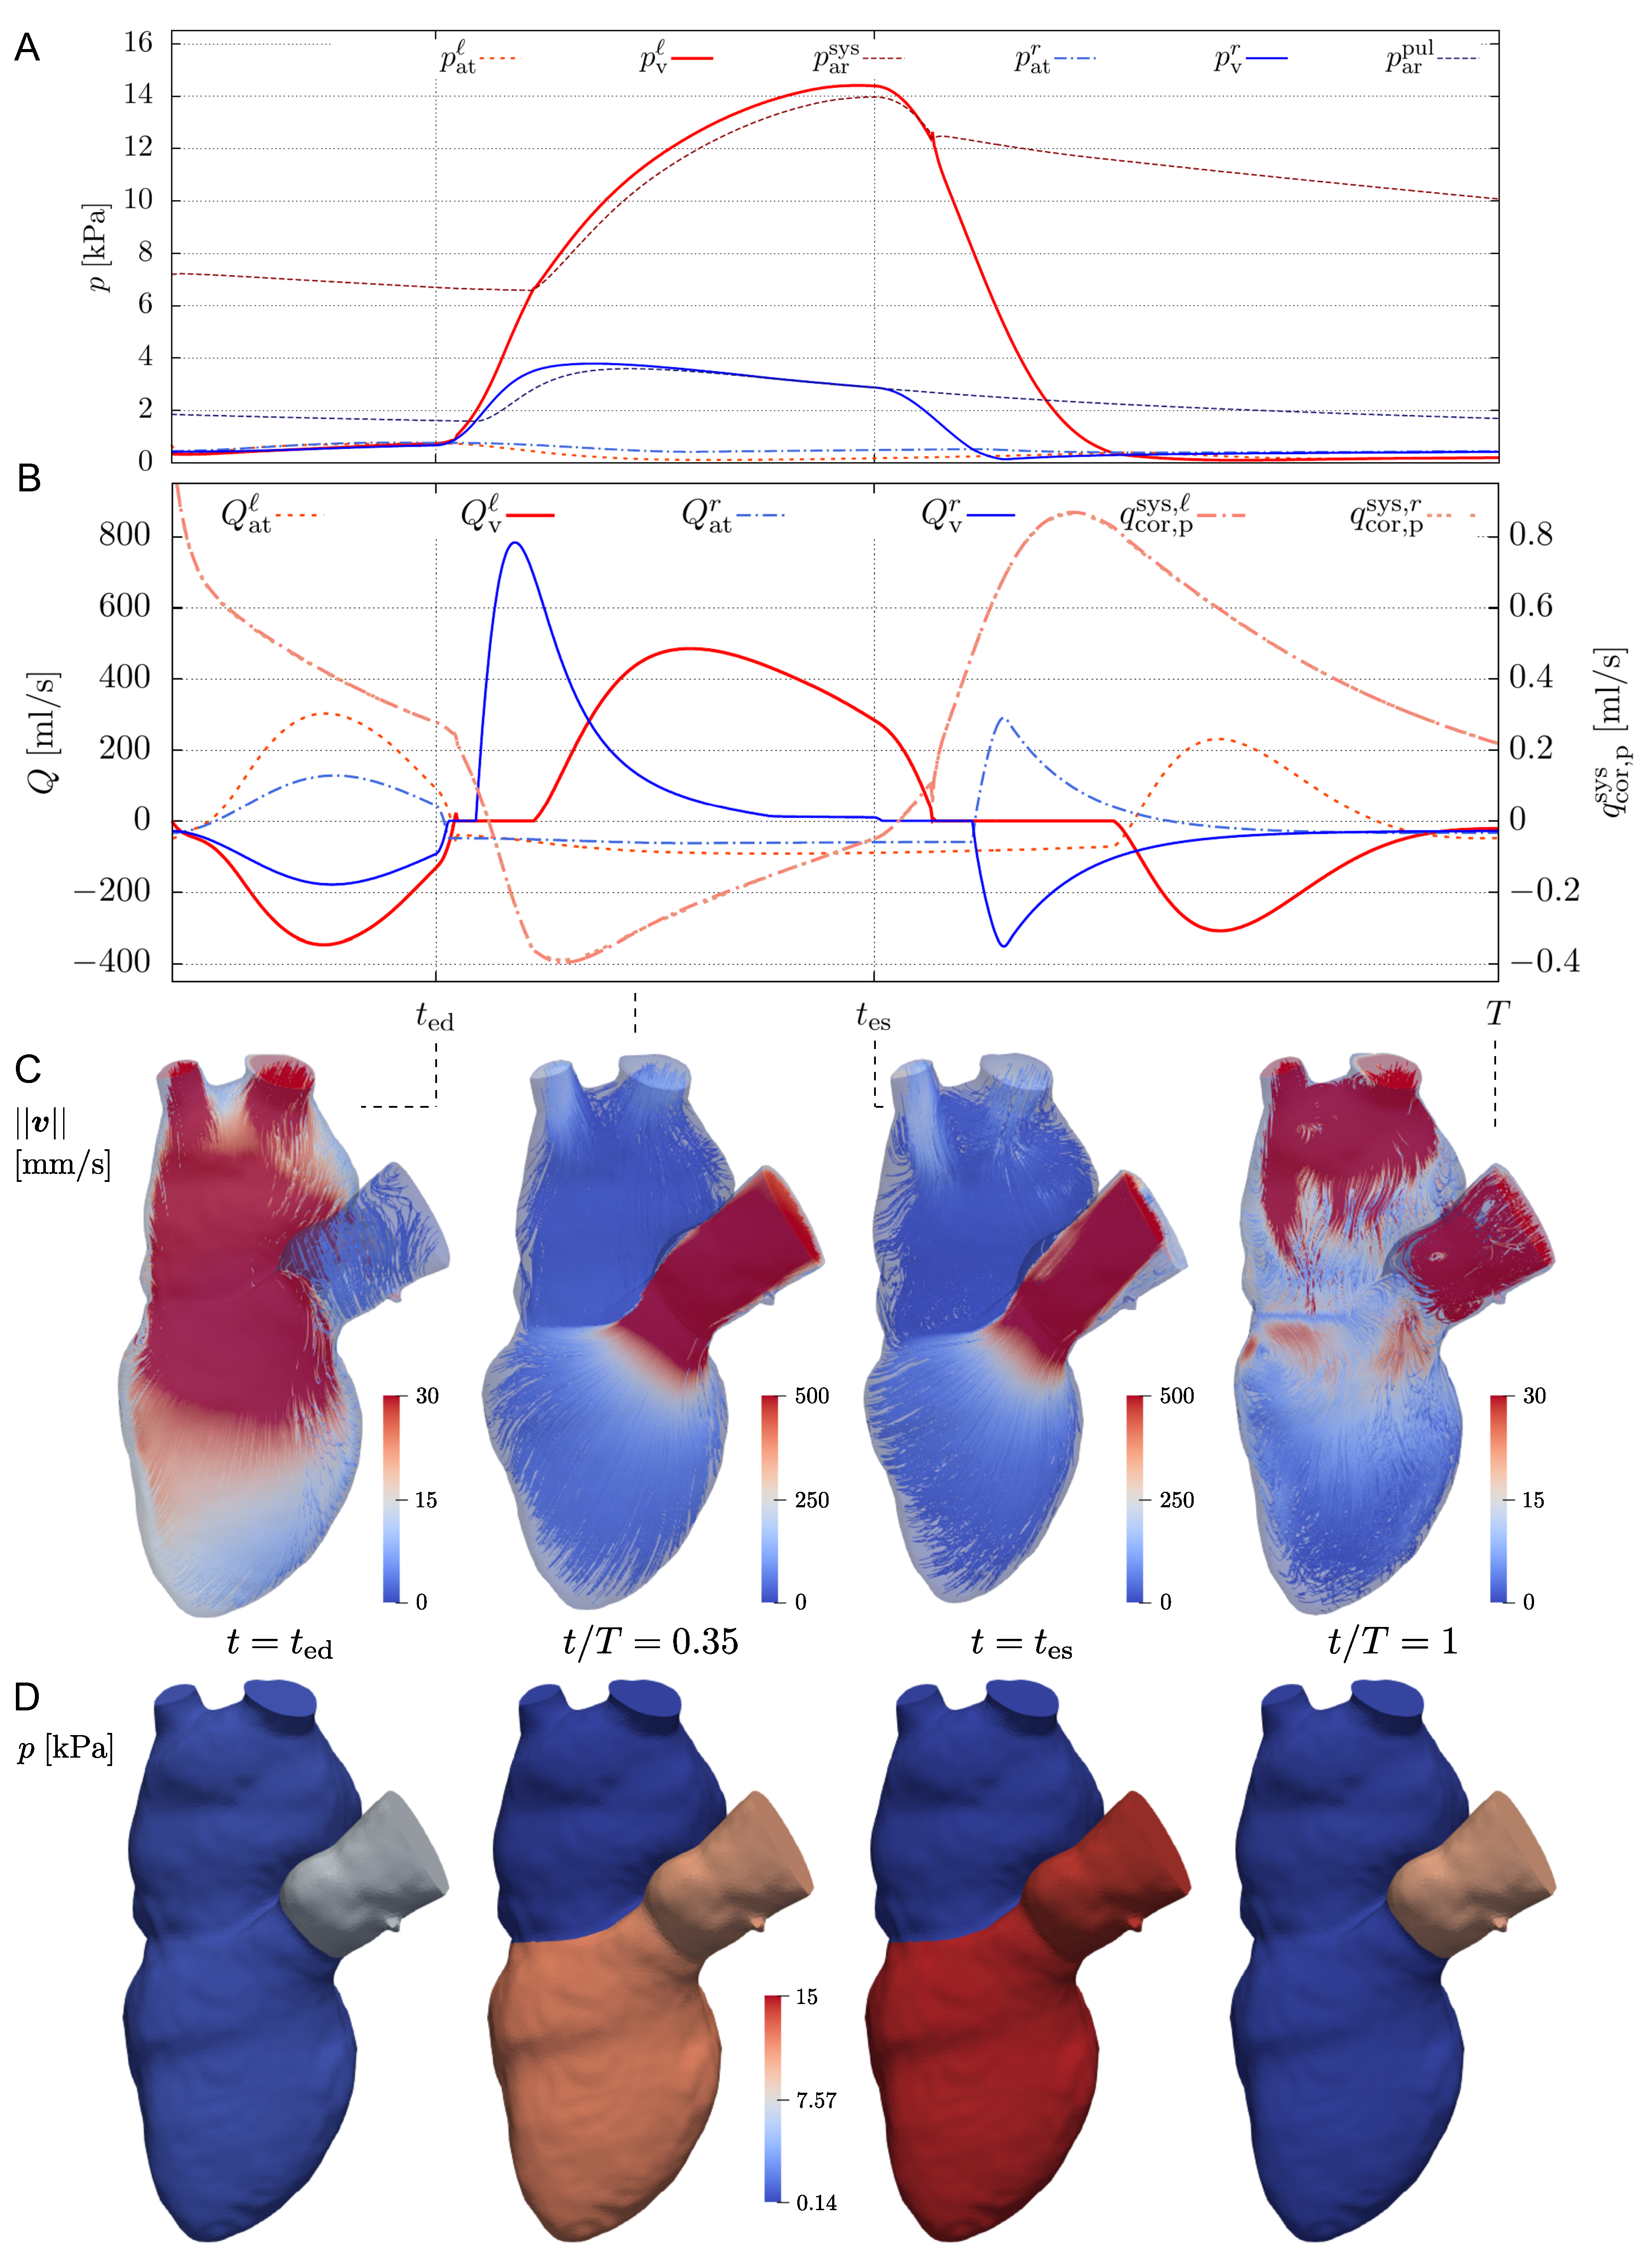
\includegraphics[width=1\textwidth]{chapters/hirschvogel/heart_results.pdf}
\caption{Adapted from \cite{hirschvogel2025-prec}: \textbf{A.} Left atrial, left ventricular, systemic arterial, right atrial, right ventricular, and pulmonary arterial pressures over time. \textbf{B.} Left atrial, left ventricular, right atrial, right ventricular, left and right proximal coronary fluxes over time. \textbf{C.} Magnitude of fluid velocity $\boldsymbol{v}$, streamlines on longitudinal cut through deformed domain $\mathit{\Omega}$. Note the different scales for diastolic and systolic snapshots. \textbf{D.} Fluid pressure $p$, plotted on undeformed reference domain $\tilde{\mathit{\Omega}}_{0}$.}\label{fig:heart_results}
\end{figure}

\section*{Conclusion}
We presented the fluid-reduced-solid interaction (FrSI) method for a patient-specific, large-scale, left heart model, with a focus on a monolithic implementation in a FEniCSx software environment. The model can represent physiologic quantities throughout a heart cycle, and may be used to predict hemodynamics under varying cardiovascular conditions, e.g. for mitral valve regurgitation and repair.

\section*{Software and data availability}
The presented results all are computed using Ambit \cite{hirschvogel2024-ambit} release version 1.3, cf. \url{https://github.com/marchirschvogel/ambit}. All data needed to run the model---the Ambit code as well as  a medium (rf1) and fine discretization (rf2, used for generating the results presented), as well as the Ambit input file---are published at \url{https://zenodo.org/records/14631793}. Running Ambit requires FEniCSx to be installed (installation instructions at \url{https://github.com/FEniCS/dolfinx}), specifically the dolfinx development version dating to Git hash \verb\4392bc84f440d7418ec4491a4a827d50720cb7d7\ (Nov 28, 2024). The model might as well run with newer dolfinx versions, however it is not tested.

\begin{acknowledgement}
DN acknowledges funding from the Engineering and Physical Sciences Research Council Healthcare Technology Challenge Award (EP/R003866/1), and support from the Wellcome Trust EPSRC Centre of Excellence in Medical Engineering (WT 088641/Z/09/Z) and the NIHR Biomedical Research Centre at Guy's and St. Thomas' NHS Foundation Trust and KCL.    
\end{acknowledgement}

\bibliographystyle{spbasic}
% Write the full path of your bibfile relative to book.tex
\bibliography{chapters/hirschvogel/bibliography.bib}


 
% Write the full path to the location of the graphics relative to book.tex
\graphicspath{{chapters/paratico/graphics/}}

\title{Estimation of optimal inlet boundary conditions for blood flow assessment in abdominal aortic aneurysm using variational data assimilation}
\titlerunning{Paratico et al.}

\author{S.~Paratico, R.~Munaf\`o, C.~Trenti, P.~ Dyverfeldt, S. Saitta and E.~Votta}
\authorrunning{Paratico et al.}

\institute{S.~Paratico \email{sara.paratico@mail.polimi.it} \at Politecnico di Milano}
\maketitle

\abstract{}
Blood fluid dynamics impacts vessel wall cells and tissue biomechanics, influencing thrombus formation and vessel wall remodeling. Accurate \textit{in vivo} quantification can thus aid in understanding these mechanisms and patient stratification. Computational fluid dynamics (CFD) and 4D flow magnetic resonance imaging (MRI) are used for this purpose, but both have limitations: CFD involves assumptions and boundary condition (BC) simplifications, while 4D flow MRI suffers from low spatial resolution and noise. This study employs variational data assimilation (VarDA) to integrate CFD and 4D flow MRI, yielding a high-resolution, noise-free flow field closely aligned with 4D flow MRI velocity data. To enhance alignment, the optimal inlet velocity profile is determined iteratively via an incremental pressure correction scheme (IPCS). Previously tested in simple synthetic geometries and later in a complex  patient-specific abdominal aortic aneurysm (AAA), this approach demonstrates improved reliability in patient-specific hemodynamic evaluation. 


\section*{Introduction}
Alterations in blood fluid dynamics often contribute to the progress of cardiovascular pathological conditions \citep{Bappoo2021,Guzzardi2015}. Hence, quantifying blood fluid dynamics on a patient-specific basis and non-invasively can support the understanding of pathological mechanisms or the stratification of patients based on the risk for adverse endpoints. To this aim, blood flow field can be reconstructed from clinical imaging, namely 4D flow magnetic resonance imaging (MRI) \citep{Dyverfeldt2015}, or computed through patient-specific computational fluid dynamics (CFD) models  \citep{Kheyfets2015}. 
However, 4D flow MRI provides indirect and noisy velocity measurements with low spatio-temporal resolution, which often violate mass conservation. CFD models solve discretized Navier-Stokes (NS) equations to compute well-resolved, noise-free velocity fields but are affected by numerical artifacts and rely on simplified boundary conditions (BCs), including inlet velocity BCs. Variational data assimilation (VarDA) integrates CFD-based NS equations with sparse, uncertain 4D flow MRI data by optimizing BCs to minimize discrepancies. In cardiovascular flows, it refines inlet velocity profiles but requires computing both velocity and pressure gradient fields, which is challenging in high-velocity arterial flows. Pressure-velocity coupling or correction schemes address this, yet MRI-induced noise can hinder proper pressure correction, affecting the accuracy of the solution.

\subsection*{Related works}
\label{sec:background}
Several studies have explored VarDA in hemodynamics, ranging from 2D steady-state to 3D transient conditions. \cite{Delia2012} showed that VarDA allows to reconstruct flow fields in geometrically complex 2D domains, such as the 2D representation of the aortic arch and carotid bifurcation, even with noisy velocity data. Subsequently, in \cite{Delia2013}, the same authors showed that, in 2D domains, noisy velocity data can be effectively managed by properly managing inlet BCs. In particular, they showed that the regularization of the inlet velocity profile through the use of a control variable also regularized the velocity field over the whole domain and allowed for successful pressure-velocity coupling. \cite{Tiago2017} extended VarDA to a 3D saccular aneurysm, demonstrating its flexibility with various BCs and optimization methods like gradient-based and genetic algorithms to improve accuracy. \cite{Koltukluoglu2018} showed that VarDA, applied to 4D Flow MRI data, outperformed traditional CFD methods by dynamically adjusting BCs in real-time to maintain flow congruence near inlets. \cite{Funke2019} demonstrated the effectiveness of 4D (3D space + time) VarDA in capturing transient blood flow in aneurysms using phase contrast-MRI data. Finally, \cite{Dokken2020} proposed a multimesh finite element (FE) method that enhanced stability and accuracy by allowing flexible BC management across multiple mesh domains, which is key for simulating complex hemodynamics in realistic geometries.

\subsection*{Aim of the work}
This study aims to implementing a method to compute \textit{in vivo} blood fluid dynamics on a patient-specific basis with high space-resolution without using simplifying hypotheses on the inlet BCs. To achieve this, VarDA is used to estimate an optimal inlet BC for CFD, starting from a noisy, uncertain 4D flow MRI-based velocity profile while enforcing consistency between the CFD-computed velocity field and sparse 4D flow MRI data in the bulk flow region. We benchmarked the method on ideal 2D and 3D geometries and then applied it to a patient-specific abdominal aortic aneurysm (AAA) geometry. 

\section*{Methods}
\label{sec:methods}

\subsection*{Data assimilation method}
The VarDA approach was formulated as an optimization problem constrained by the NS equations, using the dolfin-adjoint library for the adjoint problem. The process follows three steps: running a first numerical simulation with tentative inlet BCs (which we refer to as the \emph{forward model} or \emph{tape}), solving the optimization problem to identify inlet BCs, and running a final numerical simulation yielding the refined velocity and pressure fields (Fig. \ref{fig:scheme}).

\subsection*{Forward problem definition}
The weak and discretized form of NS equations for an incompressible fluid \citep{Stokes2009} was solved using the FE platform FEniCS \citep{Alnaes2015} to compute velocity field $\mathbf{u}$ over a domain $\Omega$ given an initial condition \(\mathbf{u}=\mathbf{u_0}\) on $\Omega$ at time $t_0$, a zero pressure condition at the outlet section $\Omega_N$ and a Dirichlet BC at the inlet section $\Omega_D$ in the form of a space- and time-dependent velocity profile $\mathbf{g}$. Through an in house Python script, 2D and 3D fluid domains $\Omega$ were discretized into triangular and tetrahedral elements, respectively, with 1-1.5 mm characteristic size and with linear and quadratic shape functions for nodal pressure and velocity, respectively. The semi-implicit Crank--Nicolson (CN) time-integration scheme was applied with a time increment of $\Delta t = 0.001$ s. The incremental pressure correction scheme (IPCS) proposed in \citep{Goda1979} was implemented. A generalized minimal residual method (GMRES) was chosen as linear solver, with tolerances of $1 \times 10^{-4}$ for momentum and continuity equations.

\subsection*{Optimization problem definition}

The optimization problem (\cref{eq:10}, constrained by the NS equations, aimed to minimize a functional $J(\mathbf{u})$ (\cref{eq:11}, defined as the difference between the computed and observed velocities. 

\begin{equation}
\small
\min_{\mathbf{c}} J(\mathbf{u}) + R(\mathbf{c}) \quad \text{s.t.} \quad F(\mathbf{u}, \mathbf{c}) = 0
\label{eq:10}
\end{equation}
\begin{equation}
\small
    J(\mathbf{u}) = \| \mathbf{u} - \mathbf{u}_{\text{obs}} \|_{L^2(\Omega)}
    \label{eq:11}
\end{equation}

To address the ill-posedness of the problem, a Tikhonov regularization term $\mathbf{R}(\mathbf{c})$ was introduced, with respect to the controlled variable defined as $c$. It accounts for two terms that are scaled by parameters \(\alpha\) and \(\beta\), where \(\beta\) is set to $0$ for steady-state conditions. This reformulation transforms the problem into an unconstrained optimization scenario, more suitable for gradient descent methods. 

\begin{equation}
\small
    \begin{aligned}
        R(\mathbf{c}) &= \| \mathbf{c} \|_{L^2(\Omega)} \\
        &\text{where} \\
        \small
        \|c\|_{\Gamma \times (0, T]} &= \left( \int_0^T \int_{\Omega} \frac{\alpha}{2} \left( \left(|\mathbf{g}_D|^2 + |\nabla \mathbf{g}_D|^2 \right) + \frac{\beta}{2} \left( |\dot{\mathbf{g}}_D|^2 +  |(\nabla \mathbf{g})_D|^2 \right) \right) \, dx \, dt \right)^{\frac{1}{2}}
    \end{aligned}
    \label{eq:12} 
\end{equation}

The adjoint approach efficiently computes the total derivative of the functional, yielding the adjoint NS equations that facilitate optimization. The iterative Broyden-Fletcher-Goldfarb-Shanno (BFGS) algorithm, in its L-BFGS variant \citep{Liu1989}, served as optimizer. The L-BFGS algorithm is already implemented in the SciPy library, which is automatically
called by dolfin-adjoint library and which provides many user-friendly numerical routines, such as the routine for optimization.


\begin{figure}
    \centering
    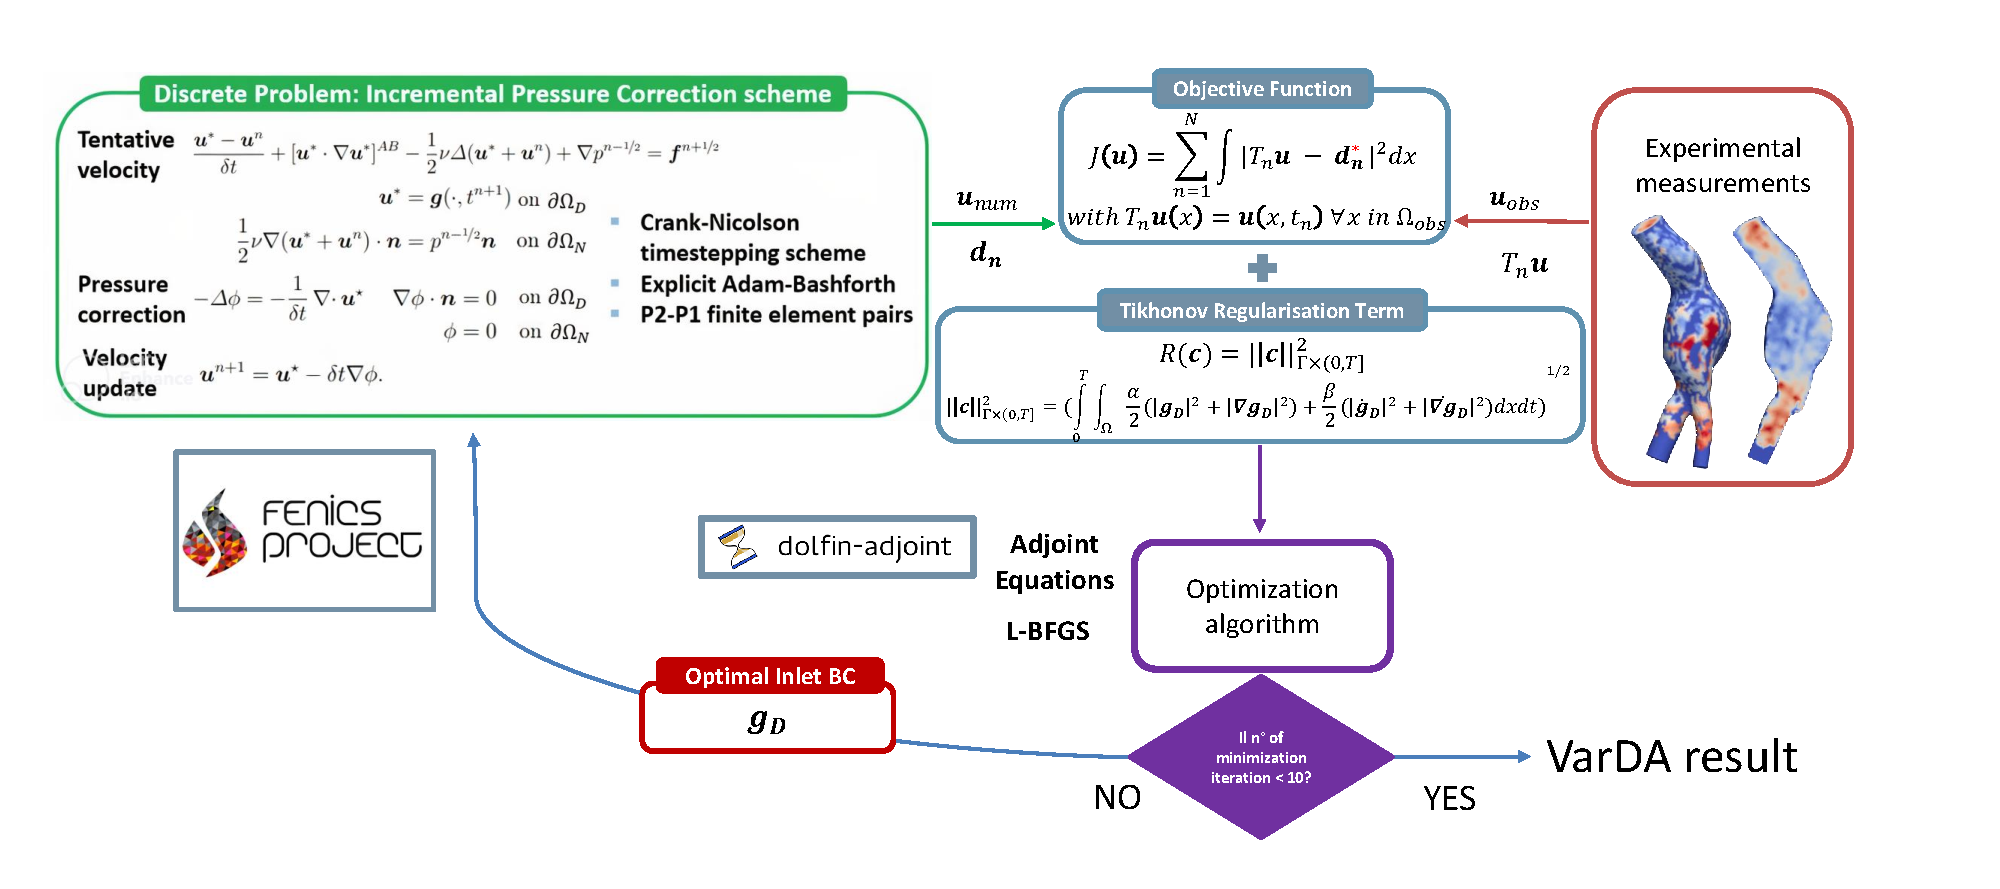
\includegraphics[width=0.95\textwidth]{chapters/paratico/Fig1.1.pdf}
    \caption{Top-left: The finite element (FE) solver computes the Navier-Stokes (NS) equations with an initial guess for the inlet boundary conditions (BCs); Top-right: experimental velocity measurements are taken at discrete points in the domain; Centre: discrepancy between the computational fluid dynamics (CFD) velocity field and experimental data is minimized by iteratively refining inlet velocity profile with a gradient-based method.}
    \label{fig:scheme}
\end{figure}

Convergence was ensured through Wolfe conditions \citep{Nocedal2006}, with maximum number of 10 iterations and ftol = $1 \times 10^{-9}$ and gtol = $1 \times 10^{-12}$ as tolerances.
The performances of the method were assessed by $J(\mathbf{u})$ value before and after optimization, Root Mean Squared Error (RMSE) between \( \mathbf{u}\) and \( \mathbf{u}_{\text{obs}} \), and qualitative analysis of the effect on the velocity field through the software Paraview.

\subsection*{Benchmark tests}

\label{sec:bench}
\subsubsection*{Preliminary tests}
First, preliminary tests were performed to compare the computational efficiency of IPCS vs. an alternative coupled scheme \citep{Figueroa2006} in a 2D straight conduit (which represents a case of 2D VarDA and can thus be addressed using the term I defined as \emph{2DVar}). Simulations were run under laminar conditions at both low and high Reynolds numbers (Re), in order to evaluate the method in laminar and transitionally unstable regimes.  
The conduit was a longitudinal section of a cylinder with a diameter of 41 mm and a length of 200 mm, made of 4,967 mesh elements. Synthetic observations (\( \mathbf{u}_{\text{obs}} \)) were generated by an auxiliary CFD simulation, prescribing a parabolic velocity profile at the inlet with peak velocity \( U_{\text{max}} = 600 \, \text{mm/s} \) (Re = 6649) and with \( U_{\text{max}} = 50 \, \text{mm/s} \) (Re = 554) for turbulent and laminar conditions, respectively.
In the tape, the tentative inlet velocity profile was parabolic with \( U_{\text{max}} = 800 \, \text{mm/s} \) (Re = 8865) and \( U_{\text{max}} = 100 \, \text{mm/s} \) (Re = 1108).
The iterative minimization of the discrepancy between \( \mathbf{u} \) and \( \mathbf{u}_{\text{obs}} \) was performed to determine the optimal velocity profile for CFD simulations, verifying if it matched the parabolic profile used to generate the synthetic observations.\\


\subsubsection*{Progressively demanding tests}
Next, the method was benchmarked through three progressively more demanding tests:

\begin{enumerate}
    \item 2D straight conduit in transient conditions (which represents a case of 2D VarDA also involving time and can thus be addressed using the term I defined as \emph{2DVar+t} benchmark) - This benchmark shared the same domain of the 2DVar benchmark. However, both the auxiliary simulation for the generation of the experimental observations and tape consisted in a sequence of two transient simulations: in the first simulation, velocity was initially equal to 0 mm/s everywhere in the domain, and at the inlet a parabolic velocity profile was imposed, whose peak velocity increased linearly from 0 to \( \frac{ U_{\text{max}}}{2} \) over 0.3 s; in the second simulation, the velocity field computed by the first one was used as IC and the inlet velocity parabolic profile was scaled by the time-dependent function \( f(t) \):

\begin{equation}
\small
f(t) = 
\begin{cases}
\frac{U_{\text{max}}}{2}\cos\left(\frac{\pi}{T_s}\left(t - \frac{T_s}{2}\right)\right), & \text{if } t \leq T_s \\
\frac{U_{\text{max}}}{2}, & \text{if } T_s < t \leq T_d
\label{eq:13}
\end{cases}
\end{equation}

where \( T_s = 300 \) ms and \( T_d = 540 \) ms are cardiac cycle's systolic and diastolic phases \citep{Katz1977}. Besides determining the optimal velocity profile for CFD simulations, spatial and temporal regularization terms [\cref{eq:12}] were incorporated into the optimization process and subjected to a sensitivity analysis.\\

    \item 3D straight conduit in steady-state conditions (which represents a case of 3D VarDA and can thus be addressed using the term I defined as \emph{3DVar} benchmark) - This benchmark evaluated the computational cost increase when transitioning from a 2D to a 3D problem. The fluid domain was a 3D cylinder with a radius of 30 mm and a length of 200 mm, made of 74,968 mesh elements. IC and BCs, as well as the objective function, were identical to those in the 2DVar benchmark.
    \item Patient-specific AAA geometry in steady-state conditions (which represents a case of 3DVar applied to a patient-specific AAA geometry and can thus be addressed using the term I defined as AAA benchmark) - This benchmark aimed to test VarDA in a complex 3D domain using real experimental observations. 4D flow imaging was acquired from an adult male with AAA using a 3T coronary magnetic resonance (CMR) system (Ingenia, Philips Healthcare, Netherlands) at Linköping University Hospital. The 4D flow data were processed with in-house Python \citep{Saitta2024} and CMR angiography was performed for 3D AAA geometry segmentation.
Two tests were carried out with laminar flow in the AAA. In the first test, observations consisted in 4DFlow data acquired during early systole, corresponding to the third time frame (about 63 ms from the start of the cardiac cycle, with a 21 ms time step), while the tape was generated by a CFD simulation fed by 4DFlow-based inlet velocity profiles. The second test assessed the method's robustness against noise, using an inlet velocity profile, scaled by 0.15, at peak systole to produce the tape's output. Noisy observations were generated by processing the tape's output according to medium noise setting of \cite{Saitta2024}.
In addition to already-mentioned metrics, wall shear stresses (WSSs) from final simulation we analyzed using custom Paraview filters.
\end{enumerate}

The associated codes can be found at the following link:
\textcolor{blue}{\url{https://github.com/saraparatico/proceedingsCodes/tree/main}.}

\section*{Results}
\label{sec:Results}
\label{ch:chapter_three}

\subsection*{Computational costs}
Numerical experiments were conducted on various setups: a workstation with 24 CPUs and 64 GB RAM for 2DVar and 3DVar and a high-performance computing system with 40 CPUs and 190 GB RAM for 2DVar+t and AAA benchmark. 2DVar took 30 minutes and 3DVar took 6 hours on 12 CPUs; on the other side, 6 hours were required for 2DVar+t and 17 hours for AAA benchmark.

\subsection*{Preliminary tests}
In high Reynolds number tests, IPCS optimization reduced RMSE from 142.60 mm/s to 6.70 mm/s, while the coupled scheme faced convergence issues. In low Reynolds conditions, IPCS proved to be five times faster than the coupled scheme and achieved a final RMSE of 1.76 mm/s compared to 4.22 mm/s for the coupled scheme.

\subsection*{Progressively demanding tests}
\subsubsection*{2DVar+t benchmark}
When a zero-velocity field was imposed as IC, the post-optimization velocity field showed inconsistencies with respect to the observations.
In particular, a high-velocity region just downstream of the inlet section was obtained, while low velocity values were computed in the rest of the domain.
Moreover, these tests did not yield improvements by changing \(\alpha\), and increasing \(\beta\) further worsened the performance (Fig. \ref{fig:3.3}).

\begin{figure}
    \centering
    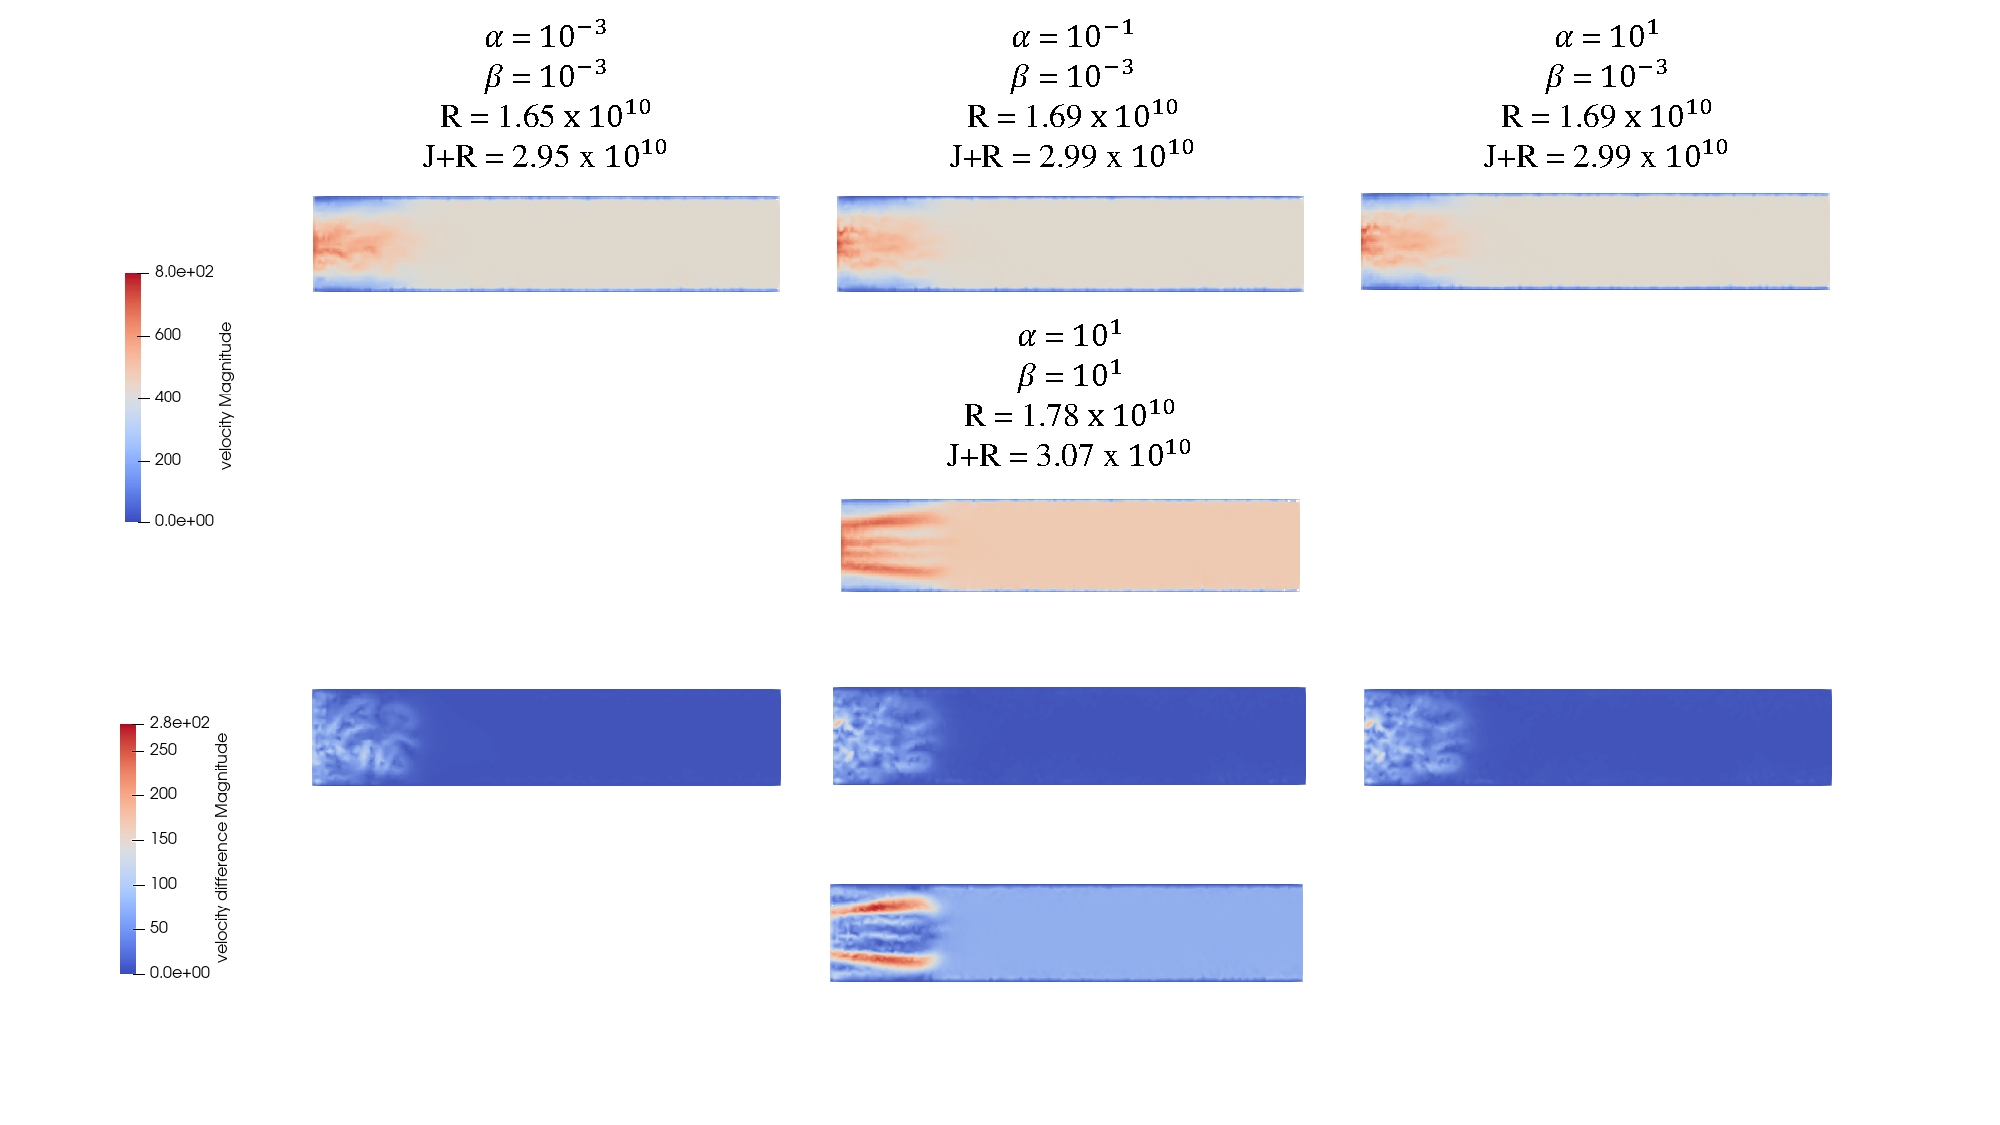
\includegraphics[width=\textwidth]{chapters/paratico/Fig1.2.pdf}
    \caption{Sensitivity analysis of regularization parameters at systolic peak. First row: 2DVar+t velocity magnitude for different $\alpha$ values ($10^{-3}$, $10^{-1}$, $10^{1}$), with $\beta = 10^{-3}$. Second row: test with $\beta = 10^{1}$ to assess time regularization. Third and fourth rows: velocity difference between reference and 3DVar results for each $\alpha$ and $\beta$.}
    \label{fig:3.3}
\end{figure}

When the initial velocity and pressure fields were set equal to those yielded by the previous post-optimization simulation, the results showed a more homogeneous flow better matching parabolic characteristics and with lower \(J + R\) values.\\

\subsubsection*{3DVar benchmark}
VarDA was performed with spatial regularization terms set to $\alpha = 10^{-2}$, $10^1$, and $10^3$. The lowest value of $J + R$ was achieved with $\alpha = 10^{-2}$, but it did not correspond to the lowest RMSE. The velocity field exhibited a peak near the inlet, suggesting continuity loss. For $\alpha = 10^1$, the lowest RMSE was achieved, and the post-optimization velocity field more accurately reflected the observed data. Increasing $\alpha$ to $10^3$ resulted in significant deviations from the observations, with unexpected velocity behaviors and higher values of $J + R$ and RMSE. This suggests that lower $\alpha$ values improve RMSE, while higher $\alpha$ values lead to smoother solutions, but can introduce inaccuracies when too large.\\


\subsubsection*{AAA benchmark}
In first tests, \(RMSE\) improved from 59.3 mm/s to 55.1 mm/s, indicating a better alignment with observations (Fig. \ref{fig:3.7a}). 
\begin{figure}
    \centering
    \begin{minipage}{\textwidth}
        \centering
        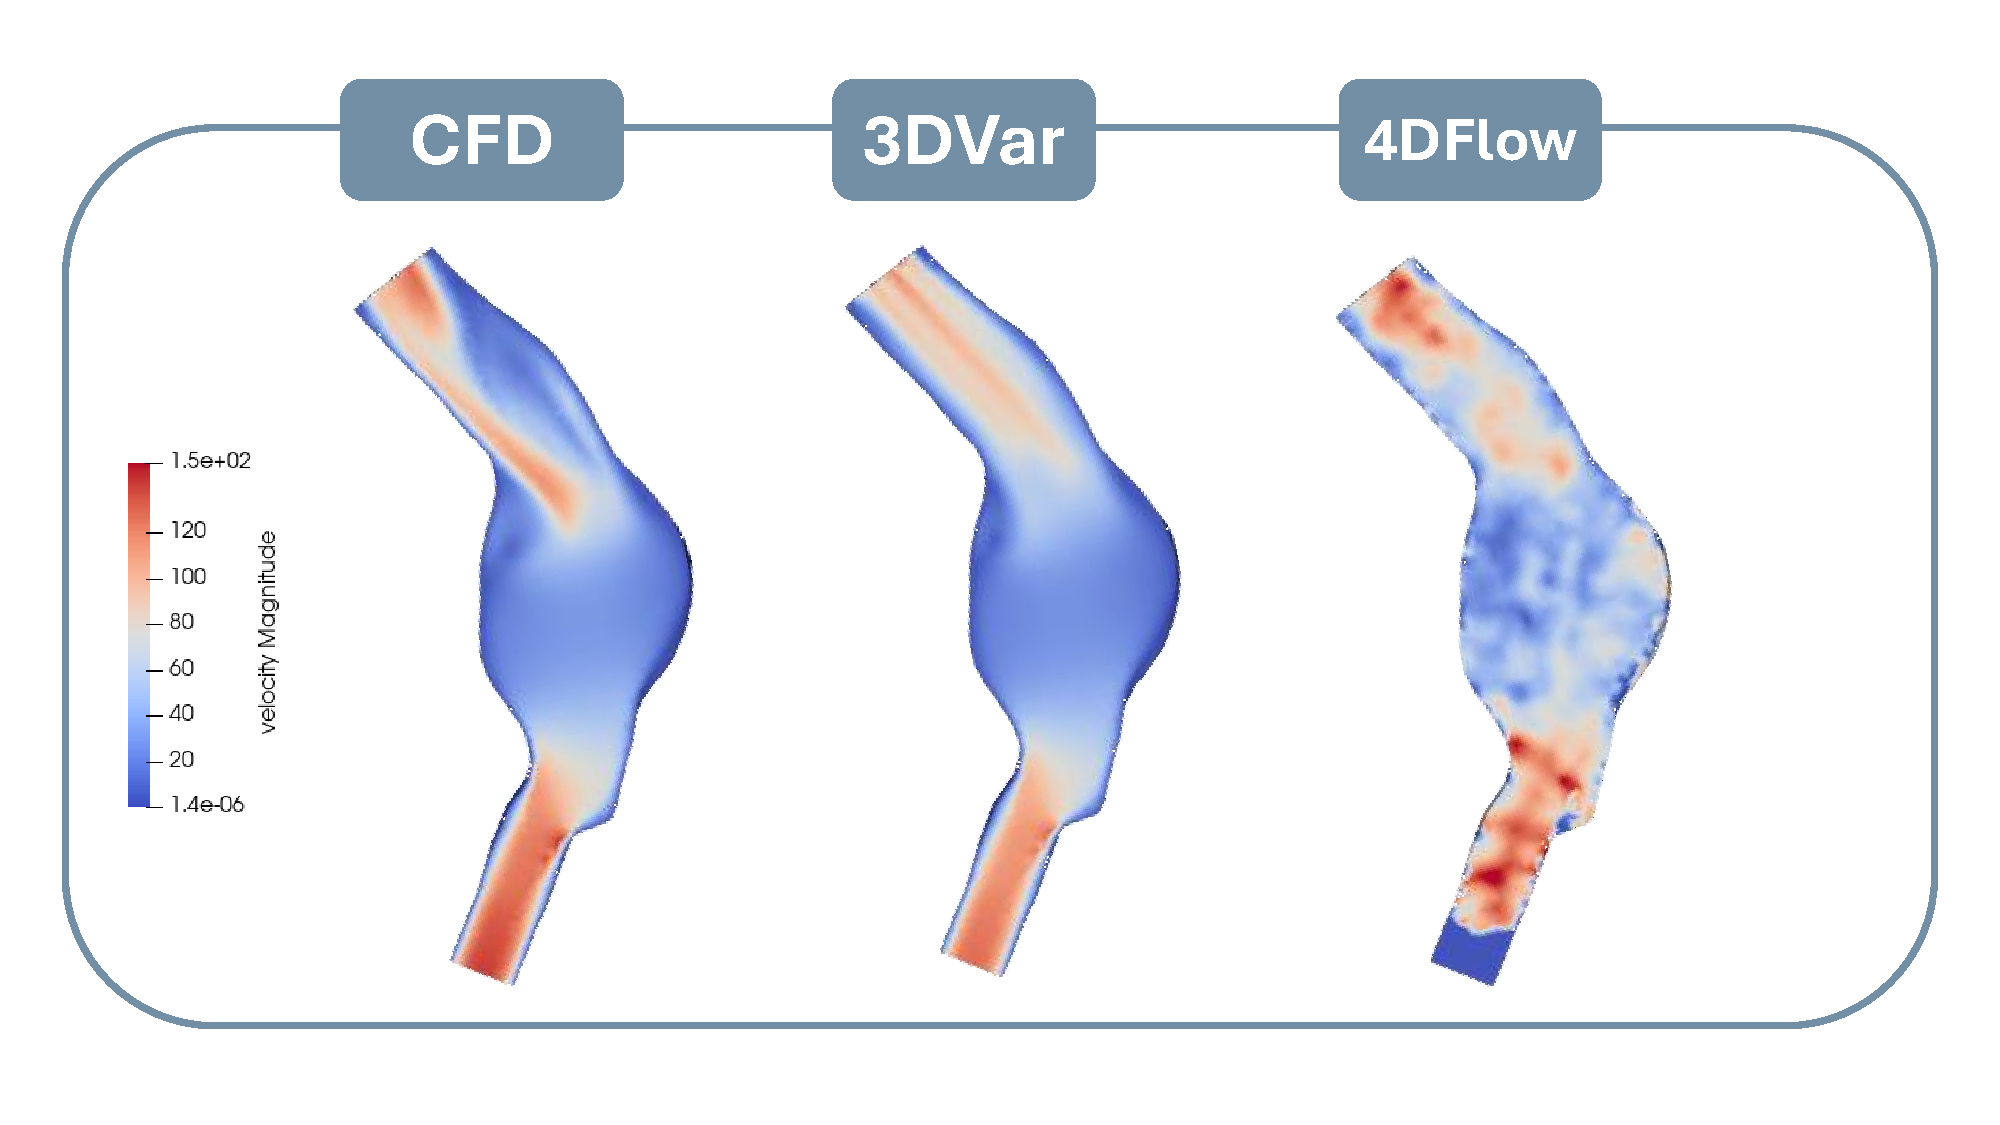
\includegraphics[width=0.9\textwidth]{chapters/paratico/Fig1.3a.pdf}
        \subcaption{\small AAA benchmark velocity magnitude maps.}
        \label{fig:3.7a}
    \end{minipage}
    \\[1em]  
    \begin{minipage}{\textwidth}
        \centering
        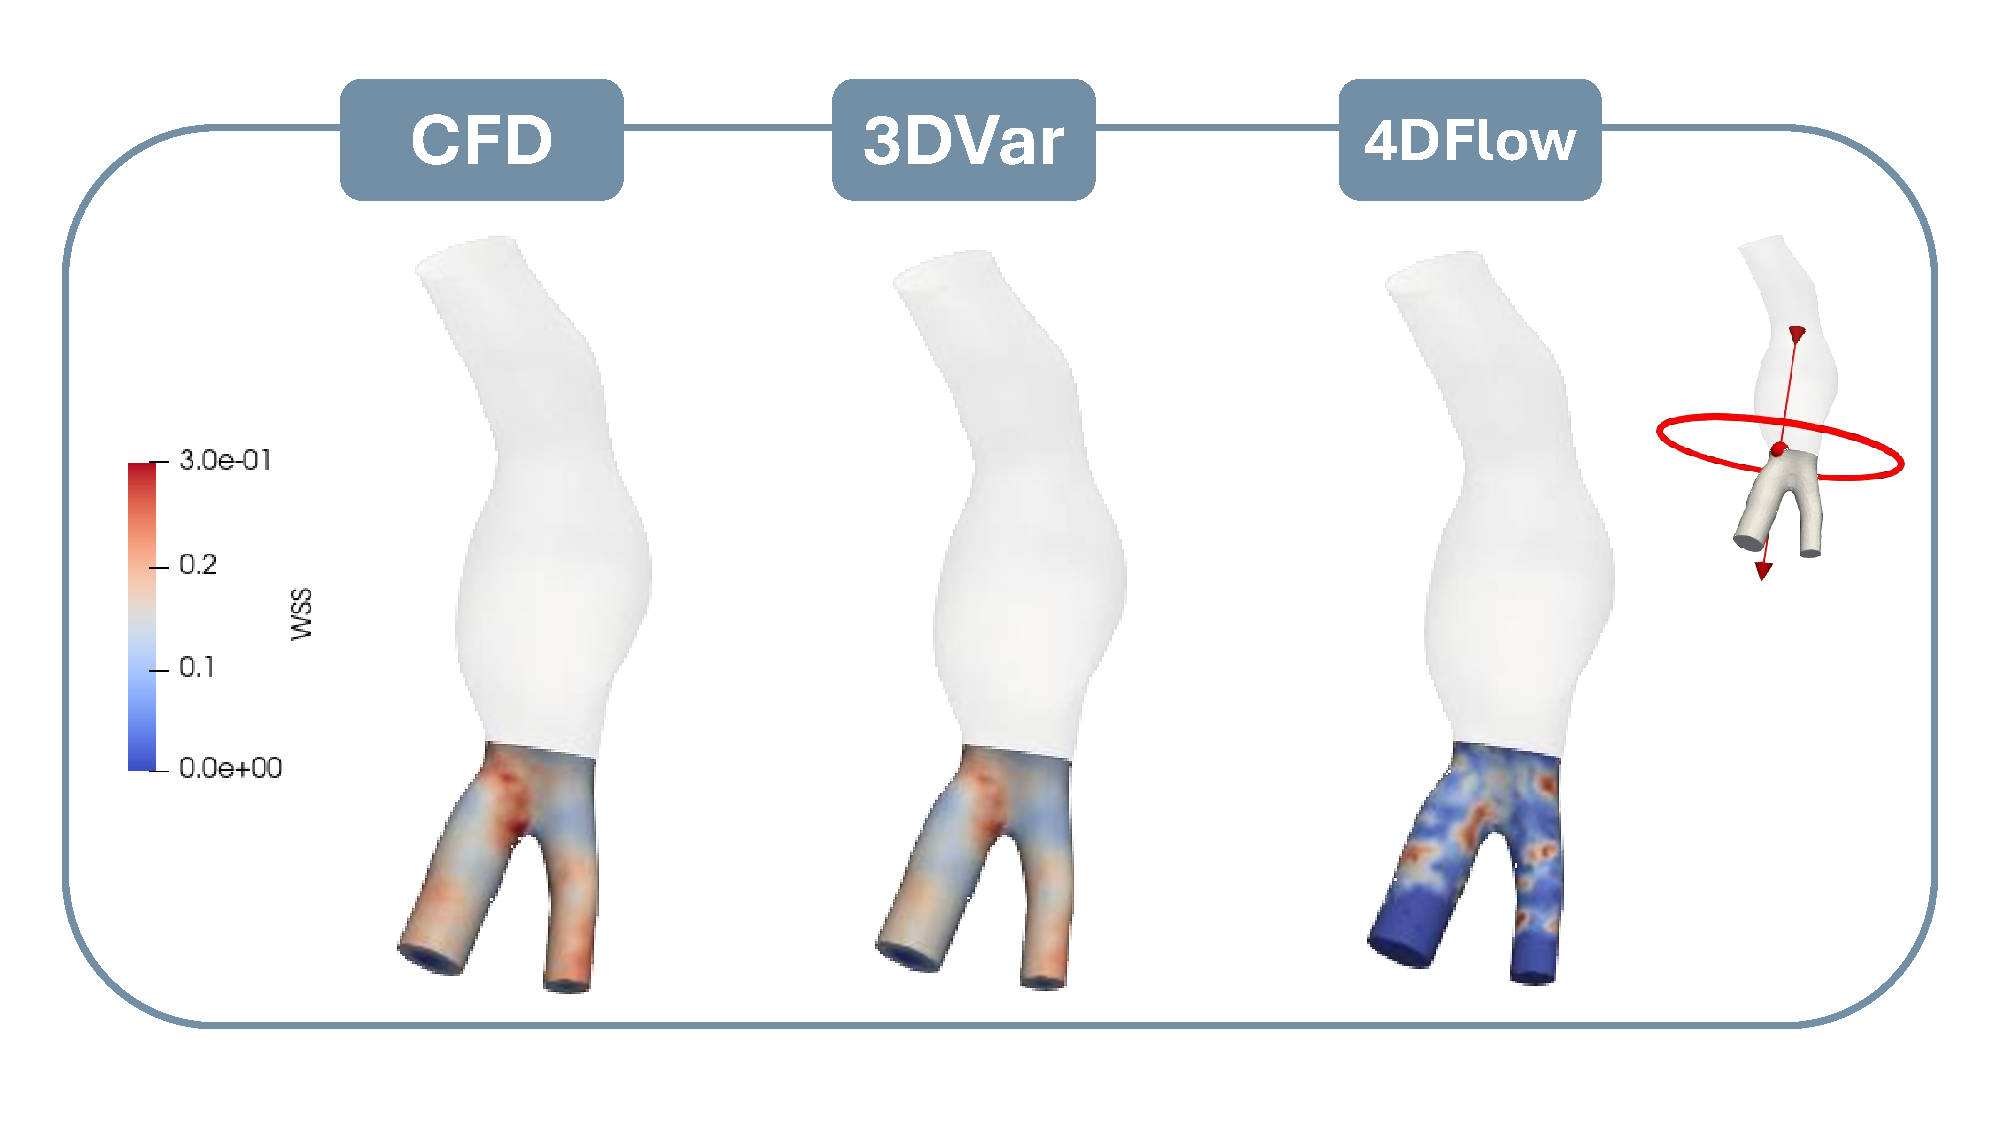
\includegraphics[width=0.9\textwidth]{chapters/paratico/Fig1.3b.pdf}
        \subcaption{\small AAA benchmark WSS maps.}
        \label{fig:3.7b}
    \end{minipage}
    \caption{\small (a) velocity and (b) wall shear stress (WSS) fields obtained on the abdominal aortic aneurysm (AAA) computed by computational fluid dynamics (CFD) (left), derived directly from 4DFlow MRI (right), and by data assimilation (centre).}
    \label{fig:3.7}
\end{figure}

Generating a tape took about 25 minutes, while optimization required 17 hours with 80 Gb of memory. WSS distributions from tape's output and 3DVar predictions were consistent, identifying regions with high shear stress (Fig. \ref{fig:3.7b}). WSS distributions from tape's output and 3DVar predictions were consistent in terms of location of high WSS regions. Moreover, while enforcing consistency with 4DFlow-based velocity measurements, the 3DVar method yielded a regular and realistic WSS distribution. This is a major difference as compared to the WSS distribution estimated directly from 4DFlow data, which was unrealistic owing to their poor space-resolution and to the impact of noise in the near-wall region. In tests with noisy observations, 3DVar effectively reconstructed the velocity field, slightly reducing \(RMSE\) from 36.8 mm/s to 36.4 mm/s, while maintaining WSS predictions consistent with CFD results, particularly at the iliac bifurcation, which is where the abdominal aorta splits into two smaller arteries, carrying blood to pelvis and legs.


\section*{Discussion}

\subsection*{From 2DVar+t to 3DVar}
The 2DVar+t reveals challenges due to inertial effects and short simulation durations, causing reconstruction defects from incomplete flow development. Extending simulation time for optimization is impractical due to high computational costs. A potential solution includes proper initialization of CFD simulations and implementing a checkpointing method to reduce computational costs by using only the last cardiac cycle for gradient calculations.
Moreover, a key difference between 2DVar+t and 3DVar is the flow field's response to regularization. In 2DVar+t, increasing $\alpha$ has minimal effect due to dominant time-dependent effects, reducing spatial regularization's impact. Additionally, increasing $\beta$ deteriorates the results, a challenge not present in 3DVar, emphasizing the difficulty of balancing temporal and spatial regularization in dynamic flows. Conversely, in 3DVar, moderate $\alpha$ values ($10^{1}$) significantly improve the velocity field, reducing inlet peaks and lowering \(RMSE\). However, excessive regularization ($\alpha = 10^{3}$) causes unrealistic velocity patterns. 

\subsection*{AAA benchmark}
AAA benchmark effectively reconstructs the velocity field in AAA geometry, maintaining high consistency with data obtained from 4D flow
imaging. It identifies high shear stress regions despite challenges due to lower resolution of 4D flow data near boundaries. The method remains robust against noise. 


\section*{Conclusions}
This study applies VarDA to estimate optimal inlet BCs for CFD using noisy 4D flow MRI data, minimizing mismatch with \textit{in vivo} velocity measurements.
The method yields a resolved, noise-free velocity field and is validated on 2D, 3D and patient-specific AAA geometries, demonstrating potential for personalized hemodynamic simulations.
The IPCS framework enhances efficiency and accuracy in transient flow analyses. Despite challenges in transient cases, this work lays the groundwork for future VarDA advancements with clinical implications.


\bibliographystyle{spbasic}
% Write the full path of your bibfile relative to book.tex
\bibliography{chapters/paratico/bibliography.bib}



% Write the full path to the location of the graphics relative to book.tex
\graphicspath{{chapters/zhang/graphics/}}


\title{Thermal analysis of brake discs in rail vehicles}
\titlerunning{Thermal analysis}

\author{Yanjun Zhang, Sebastian Stichel and William Liu}
\authorrunning{Yanjun et al.}

\institute{Yanjun Zhang \email{yanjunzh@kth.se} \at KTH Royal Institute of Technology}

\maketitle

\abstract{}
Railway brake discs convert the kinetic energy of rail vehicles to thermal energy to achieve braking. This thermal energy deteriorates braking performance, therefore, it is necessary to conduct thermal analyses of brake discs. In this work, we build a FEM (finite element method) model in FEniCSx to investigate the influence of contact areas between brake pads and discs on the temperature of brake discs. The weak form of the nonlinear heat transfer equation has been derived, which accounts for conduction, convection and radiation. Multiple Neumann boundary conditions are applied. Simulation results are validated with experimental results. With this efficient FEM model, more advanced research related to railway brake discs can be conducted, such as investigating the effect of wear and thermal expansion, or designing a new geometry of the brake pads and discs.

\section*{Introduction}
Rail vehicles are developed towards higher speed and higher axle load, requiring robust mechanical brake systems for running safety. As shown in figure \ref{fig:disc_block}, one of the most important mechanical brake systems is the disc brake, which converts the kinetic energy of the rail vehicle into heat. A high brake disc temperature reduces the coefficient of friction between the brake discs and the brake pads \cite{Saffar2010}, and causes high thermal stress, which, in turn, induces thermal cracks on the brake discs. To avoid these negative impacts, it is necessary to study the temperature distribution of brake discs. Experimental investigation is relatively complex and can not obtain some parameters, while numerical study is an effective way to address this issue.

\begin{figure}[h]
    \centering
    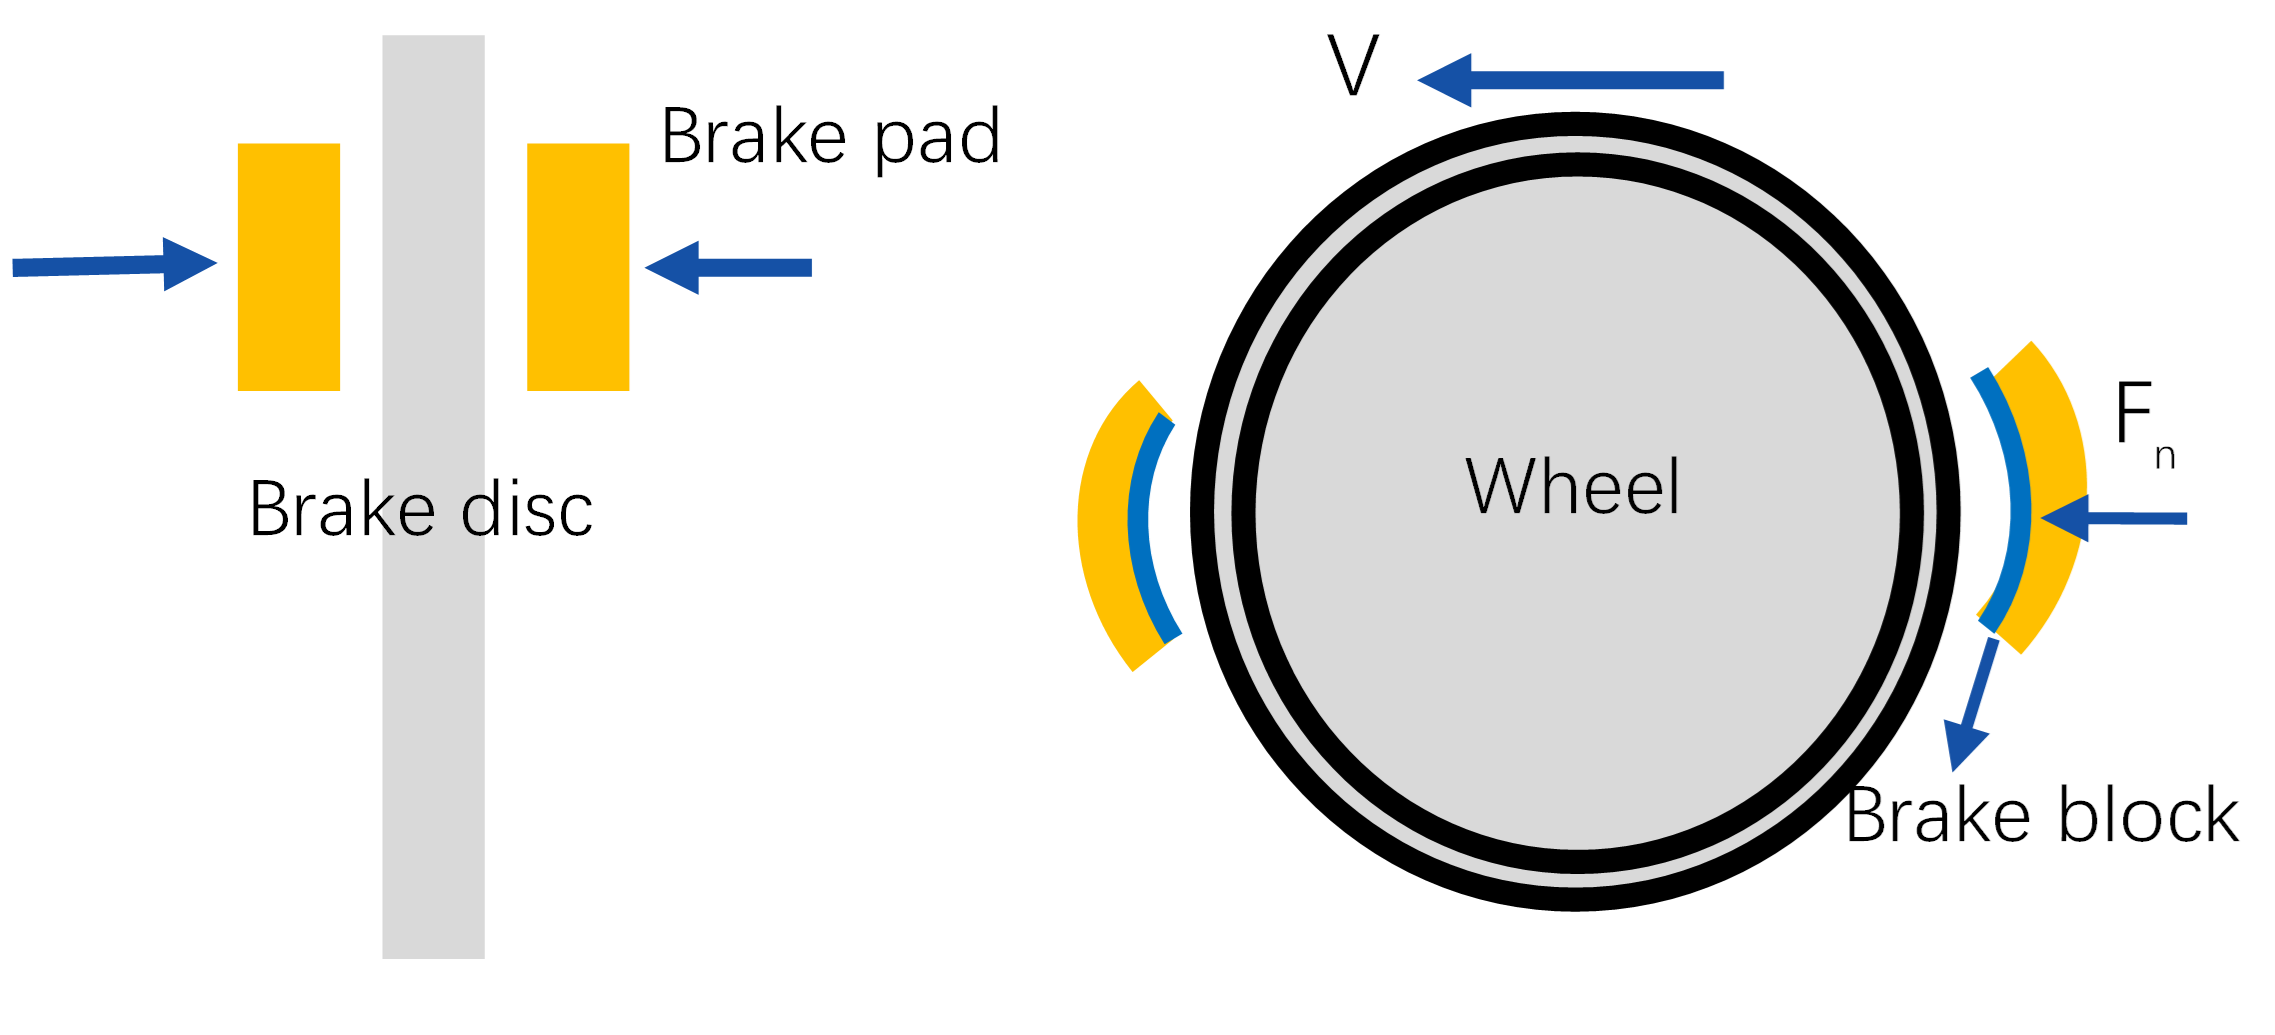
\includegraphics[width=0.65\textwidth]{chapters/zhang/graphics/disc_block_brakes.png}
    \caption{Block and disc brakes for rail vehicles}
    \label{fig:disc_block}
\end{figure}

Most thermal analyses of brake discs assume full contact between the brake pads and discs. From tribology studies, the real contact area is around 20\% of the whole brake pad friction surface \cite{eriksson_nature_2002}. Because of thermal expansion and wear of the brake pads, the contact area between the brake pads and discs is always changing. It is difficult to predict the true contact area. However, assuming fixed contact areas, the effect on the temperatures of brake discs can be investigated. This research aims to address the effects of different contact areas on the temperature of the brake discs.



\section*{Methods}

\subsection*{Modelling}
Heat generation and dissipation are two main parts of conducting thermal analysis of railway brake discs. Heat flux is based on friction
\begin{equation}
    q_d = \xi F_f V = \xi P A_d \mu V, 
    \label{heat flux}
\end{equation}

where \( q_d \) is the heat flux in the brake discs (W/m$^2$), \( \xi \) is the heat partition coefficient, \( F_f \) is the friction force (N), \( V \) is the velocity (m/s), \( P \) is the local contact pressure between the brake pads and discs (Pa), \( A_d \) is the friction contact area of the brake pads (m$^2$), and \( \mu \) is the coefficient of friction. Equation \ref{heat flux} is the Neumann boundary condition of Equation \ref{heat equation}, which is the overall heat transfer equation.

The heat flux distribution between the brake pads and discs is vital since it depends on how much heat flows to brake discs, which affects the temperatures and stresses. This coefficient is highly non-linear, affected by material, temperature, and pressure. In this research, this coefficient is simplified to a constant number. The distribution factor is described by \cite{rudolf_limpert_brake_1999}
\begin{equation}
    \xi = \frac{q_p}{q_d + q_p},
\end{equation}
where \( q_p \) is the heat flux in the brake pads (W/m$^2$), and \( q_d \) is the heat flux in the brake discs (W/m$^2$). 

The next step is to build a FEM model of the brake disc. FEM is a method to solve partial differential equations. This method includes the discrete domain, uses an appropriate basis, and rewrites algebraic equations. The heat equation is 
\begin{equation}
    \rho c \frac{\partial T}{\partial t} + \nabla \cdot (- k \nabla T) = f,
    \label{heat equation}
\end{equation}
where \( \rho \) is density, \( c \) is thermal capacity, \( T \) is temperature, \( t \) is time, \( k \) is the overall heat transfer coefficient, and \( f \) is the inner heat source. The time derivative on the right-hand side can be approximated by a difference quotient. Here we use the Euler backward method for consideration of numerical stability. After that, all items are multiplied by a test function \( v \) and integrated by parts. Then according to the divergence theorem, the bilinear form \( a(T,v) \) and linear form \( L(v) \) are

\begin{equation}
    a(T,v) = \frac{\rho c}{\Delta t} \int_\Omega T v dx + \int_\Omega k \nabla T \cdot \nabla v dx + \int_{\partial \Omega} h T v ds + \int_{\partial \Omega} \epsilon \sigma T^4 v ds,
\end{equation}

\begin{equation}
    L_{n+1}(v) = \int_\Omega f^{n+1} v dx 
    + \frac{\rho c}{\Delta t} \int_\Omega  T^{n} v dx 
    -  \int_{\partial \Omega} q v ds
    +  \int_{\partial \Omega} h T_a v ds 
    + \int_{\partial \Omega} \epsilon \sigma T_a^4 v ds,
\end{equation}
where \( \Omega \) is the computation domain, \( \partial \Omega \) is the boundary, \( dx \) is the differential element for integration over the domain, and \( ds \) is the differential element for integration over the boundary, \( h \) is the heat convection coefficient,  \(\Delta t\)\ is the time step, \(n\) is an integer counting time levels. The thermal radiation equation is based on Stefan-Boltzmann Law, where \( \epsilon \) is the emissivity, \( \sigma \) is Stefan-Boltzmann constant, \(T\) is the temperature and \(T^4\) is the temperature to the power of four, \( T_a \) is ambient temperature. For more detailed derivation, please see \cite{zhang_heat_transfer2024}.

The above equation is only for heat transfer, as for brake pad deformation, one needs to solve the elastic equation and here we haven't included here. The main contribution of the elastic deformation calculation is a more accurate contact area between the brake pads and the discs. In this study, we assume that the contact area is known a priori since this research focuses on comparing the influence of different contact areas. The above equations are solved in the FEniCSx platform \cite{baratta_dolfinx_2023,scroggs_construction_2022,alnaes_unified_2014}. All the codes for this paper are in \cite{zhang_thermal_2025}.

The computation domain or mesh is shown in Figure \ref{fig:coarse mesh}. This is a much coarser mesh than the one with 1 million elements used later, with around 43,000 elements. The element type is tetrahedron since when we compared it with hexahedral elements, we found with more tetrahedron elements, the simulation can get the same accuracy with hexahedral elements while tetrahedron has less computation time. Only the brake disc and pad are computation domains. The friction heat, or the Neumann boundary condition is applied on the contact surface, more specifically, only the rubbing elements of the brake pad areas. The rubbing elements are the column structure of the brake pad. Other boundaries include radiation and convection heat transfer, which are also the Neumann boundary conditions without the heat flux input. In each time step, the boundary conditions are redefined since the rotation will change the contact area. In reality, the brake pad should keep still while the brake disc rotates. Here we assumed only the heat flux input areas are rotating: these are the friction heat input areas.

\begin{figure}[h]
    \centering
    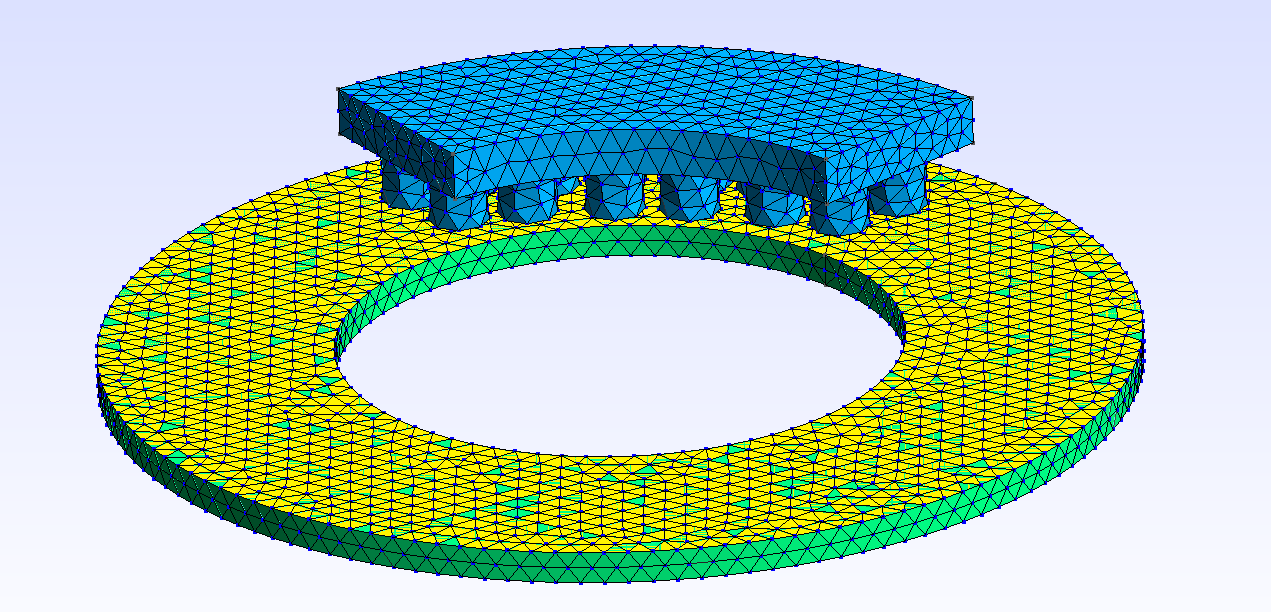
\includegraphics[width=0.9\textwidth]{chapters/zhang/graphics/3d surface.png}
    \caption{Computation domain of brake pad and disc, the mesh is much coarser than 1 million case. Friction heat or the Neumann boundary condition is only applied to friction contact areas.}
    \label{fig:coarse mesh}
\end{figure}


\subsection*{Experiment}

The test rig mainly consists of a DC motor, flywheels, brake pad and brake disc, as shown in Figure \ref{fig:test rig}. The maximum motor power is 450 kW, and the maximum motor torque is 4000 Nm. The brake pressure at the reservoir ranges from 0-10 Bar. 
There are in total 6 thermocouples to measure the temperature of the brake disc, which are located under the contact surface. A symmetric model is used in the simulation to save computational effort. The brake lag is the time it takes for the brake pressure to increase from 0\% to 95\% of the target pressure. In the test, the brake lag is 4±0.2 s, which follows the UIC 541-3 standard. Table \ref{tab: operational parameters} shows the operational parameters.

\begin{figure}[h]
    \centering
    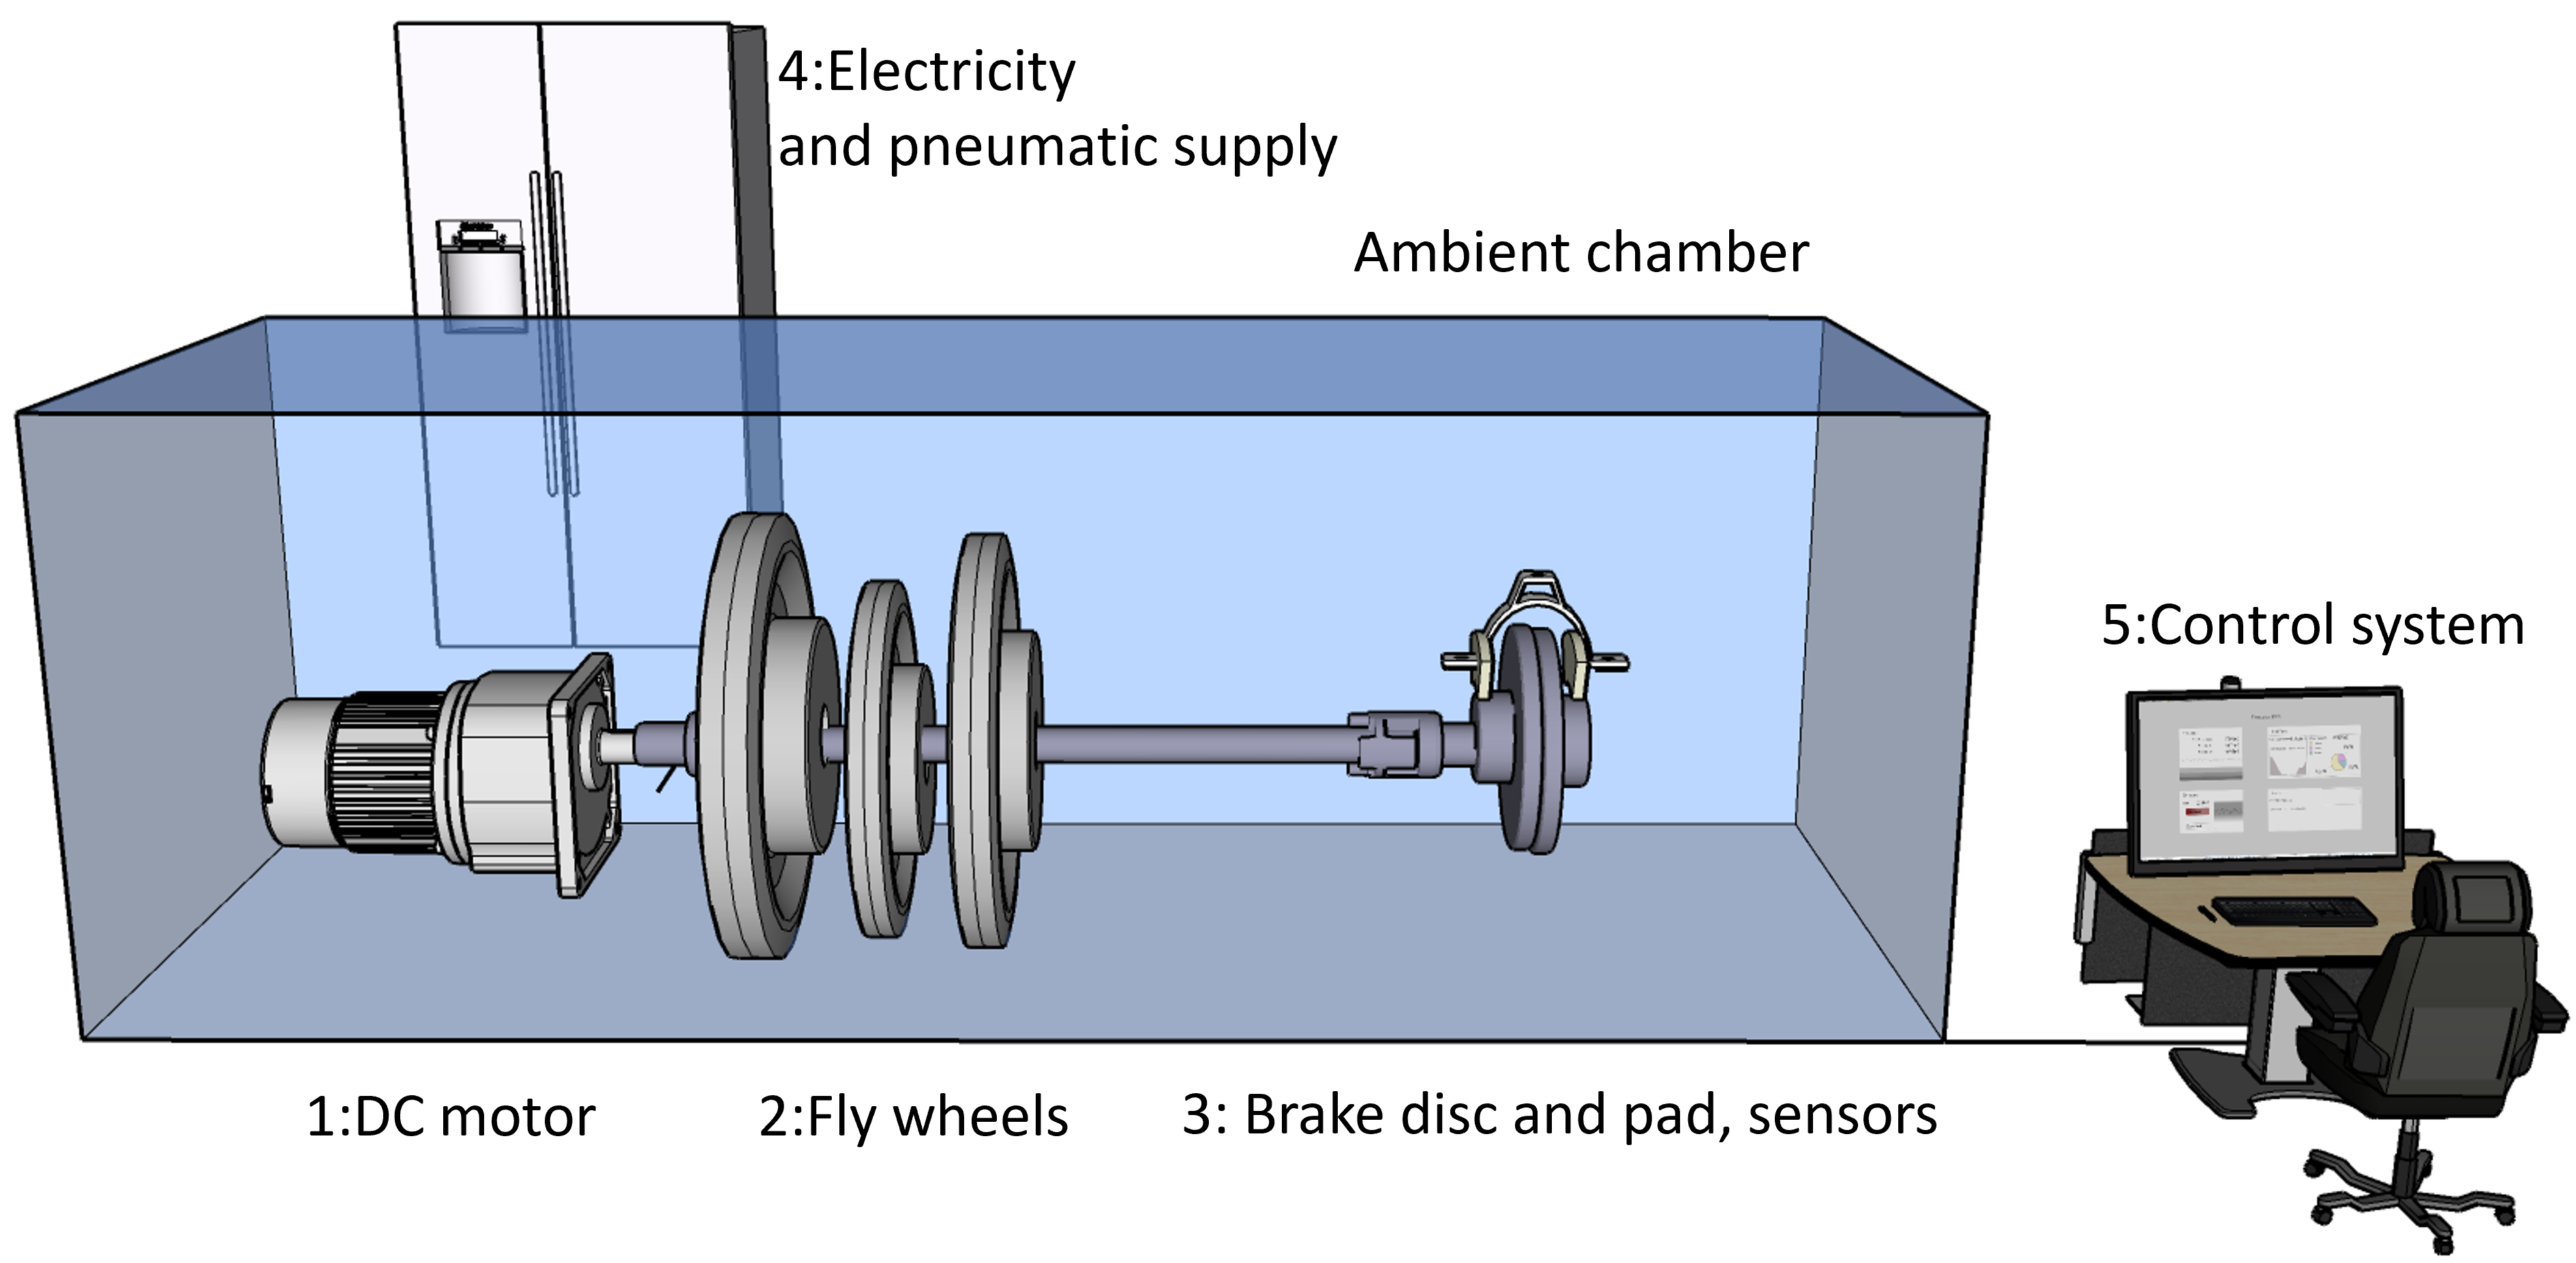
\includegraphics[width=0.85\textwidth]{chapters/zhang/graphics/test_rig.png}
    \caption{Full scale railway brake test rig}
    \label{fig:test rig}
\end{figure}

\begin{table}[h]
    \centering
    \begin{tabular}{llll} % 'l' for left-aligned, 'c' for centered
        \toprule
        \textbf{property} & \textbf{quantity} & \textbf{property} & \textbf{quantity}\\ % Header row
        \midrule
        initial velocity (km/h)             & 160       &braking time(s)          & 49 \\
        contact pressure (MPa)              & 0.274      &coefficient of friction  & 0.376 \\
        heat transfer coefficient( W/(m·k)) & 30-125    &heat distributor factor  & 0.88 \\
        brake lag (s)                       & 4         &initial temperature ($^\circ\text{C}$) & 50\\
       
        \bottomrule
    \end{tabular}
    \caption{Brake test parameters}
    \label{tab: operational parameters}
\end{table}

\begin{figure}[h]
    \centering
    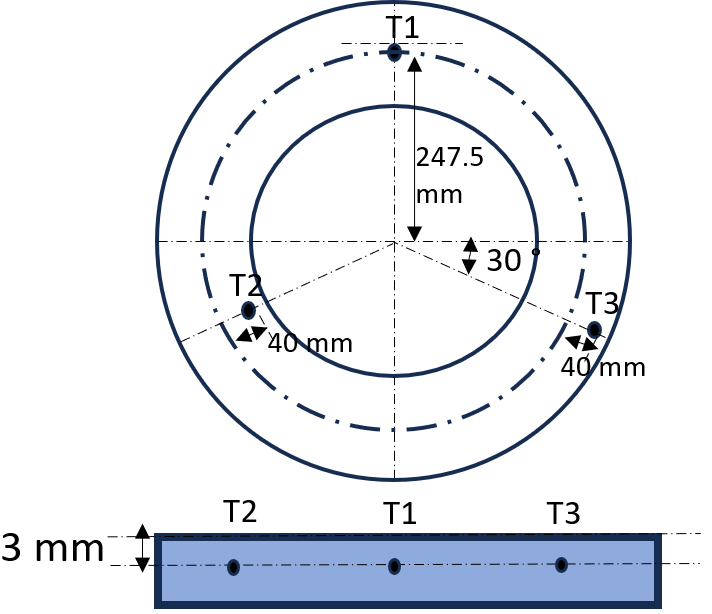
\includegraphics[width=0.45\textwidth]{chapters/zhang/graphics/thermo_couples.png}
    \caption{Location of three thermocouples}
    \label{fig:thermocouples}
\end{figure}


\section*{Results and discussion}

\subsection*{Validation}
The first step is mesh sensitivity and time step analysis, where we aim to show that the simulation results converge with finer mesh sizes and smaller time steps. Since no exact solution exist, the average temperature of point T1, as shown in Figure \ref{fig:thermocouples} is used as the convergence parameter.
\begin{figure}
    \centering
    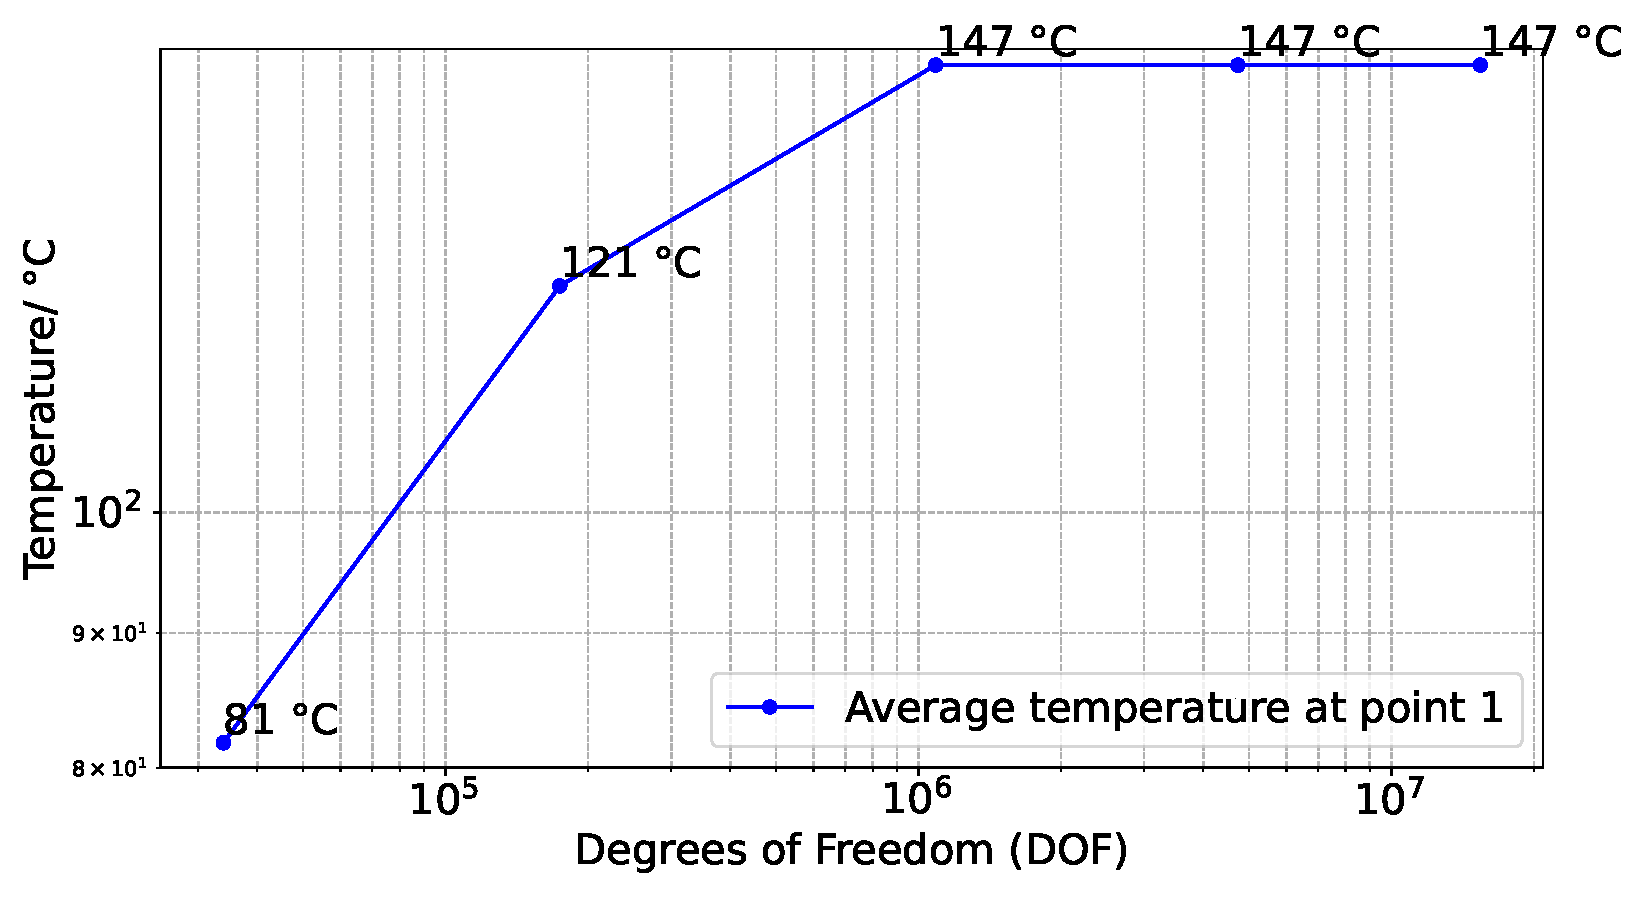
\includegraphics[width=0.8\linewidth]{chapters/zhang/graphics/ave_T_vs_dof.pdf}
    \caption{Convergence test, average temperatures of point T1, compared with degrees of freedom (DOFs)}
    \label{fig:error_mesh}
\end{figure}

 As shown in Figure \ref{fig:error_mesh}, the average temperature of point T1 increases with more degrees of freedom until 1 million degrees of freedom (DOFs). Above 1 million, the temperature remains constant.  The above results show that DOFs above 1 million are enough to capture the characteristics of the system. 
\begin{figure}[h]
    \centering
  
    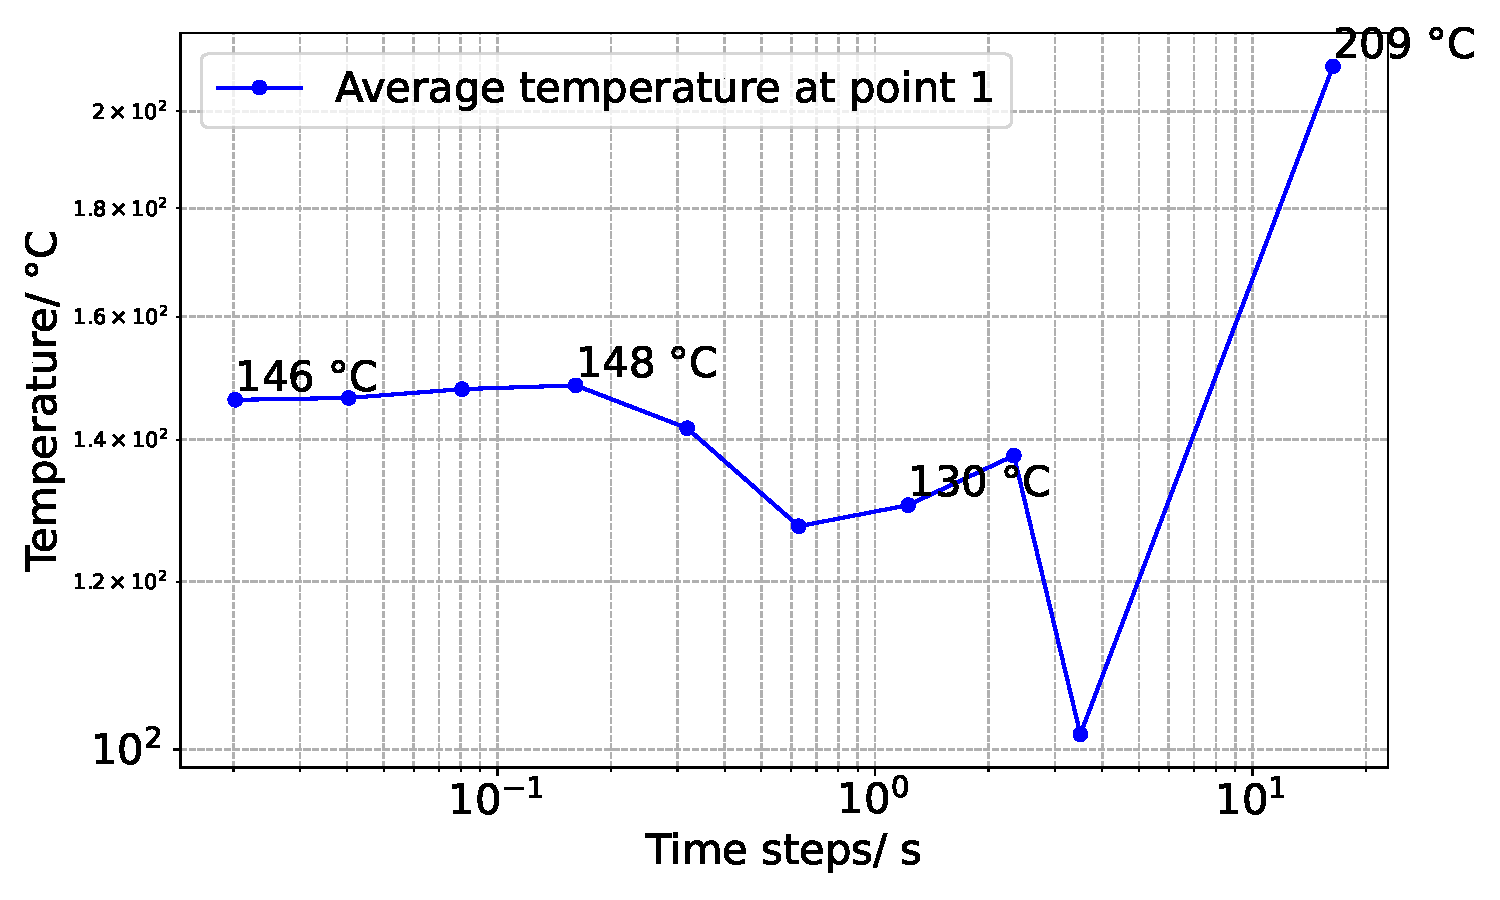
\includegraphics[width=0.8\textwidth]{chapters/zhang/graphics/T_ave_vs_dt.pdf}
    \caption{Convergence test, average temperatures of point T1 with time step}
    \label{fig:error_time}
\end{figure}


Figure \ref{fig:error_time} is a comparison of the average temperature of point 1 and times steps. When \(dt\) is above 1 s, the temperature has a large variance. The best value of \(dt\) is 0.16 s (point of 148$^{\circ}\text{C}$ ), which is a balance time step between accuracy and computational time.

\begin{figure}[h]
    \centering
    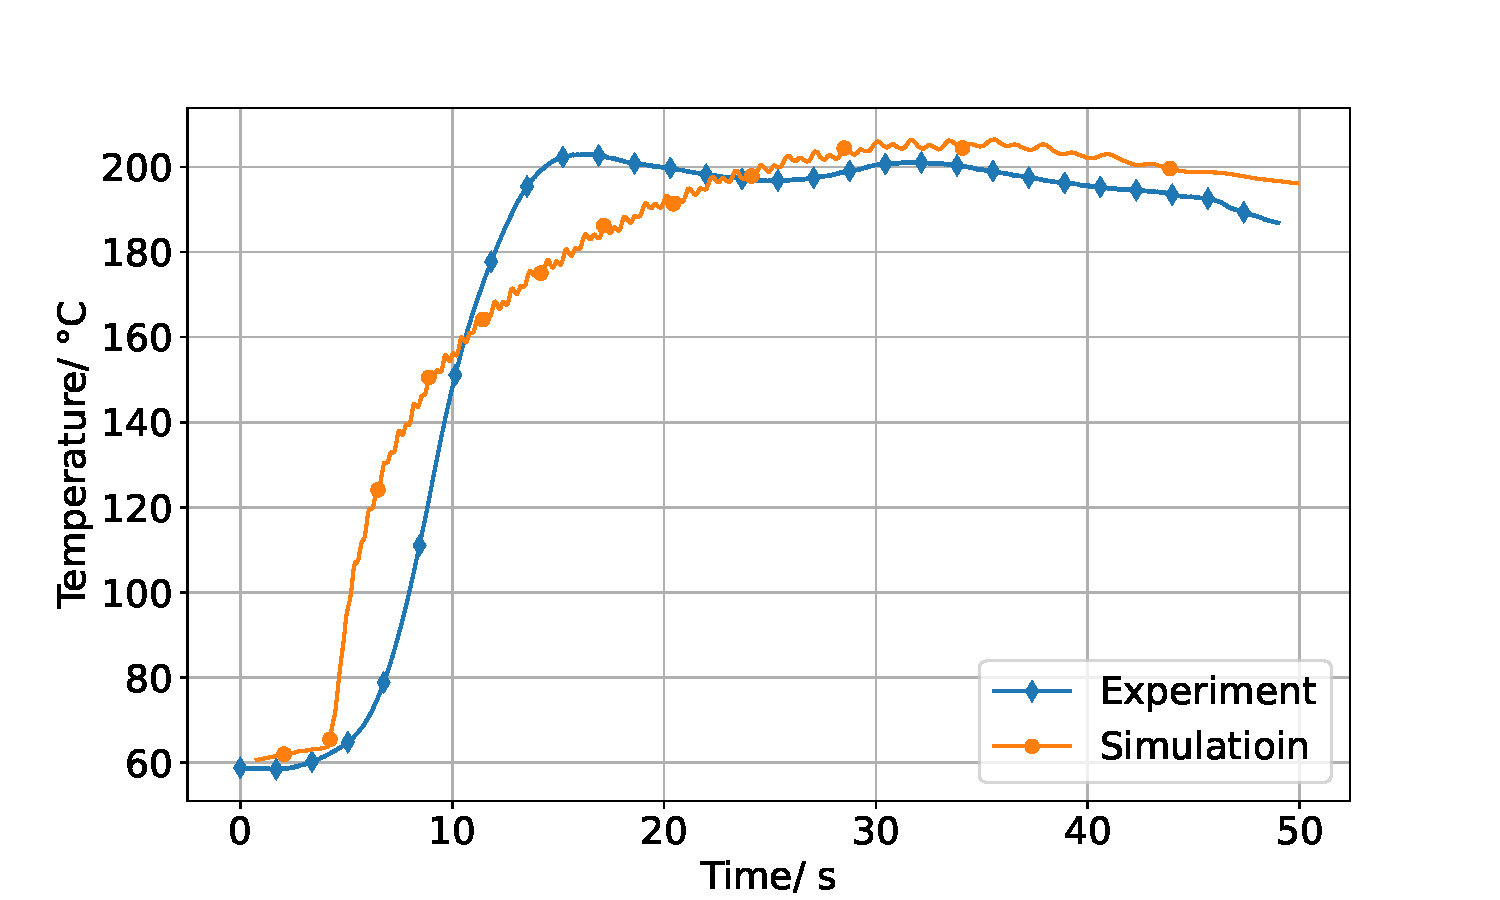
\includegraphics[width=0.8\textwidth]{chapters/zhang/graphics/T_sim_exe.pdf}
    \caption{Comparison between simulation time and experimental results}
    \label{fig:experiment}
\end{figure}

Except for mesh and time sensitivities analysis, the simulation results should validated against the experiment. As shown in Figure \ref{fig:experiment}. The general trend of case 1.2 million elements(4.7 million DOFs) and measurement data are the same, so we think the simulation accuracy is acceptable. However, there is still a large space to improve the accuracy. Such as introducing nonlinear material properties. These parameters, such as thermal conductivity, heat capacity, and coefficient of friction are all not constant or linear with temperature, velocity, and pressure. Getting the exact material characteristics is difficult. So better numerical results can benefit from the research of tribology and material engineering. The more detailed experiment parameters, like the loading pressure, would also significantly improve the numerical results since the experiment tests also contain large variances.



\subsection*{Average and maximum temperatures}

This section presents the temperatures of brake discs with different contact areas. The average and the maximum temperatures are presented.
The total contact surface is 200 cm$^2$. The brake pressures from the back of the brake pads are the same, 0.274 MPa, while the different contact areas will affect the contact pressure between the brake pads and discs. 20\%, 50\% and 100\% contact areas are compared. The 20\% contact areas represent the research from Eriksson \cite{eriksson_nature_2002}, and the 100\% contact areas represent most FEM or analytical solutions.

\begin{figure}[h]
    \centering
    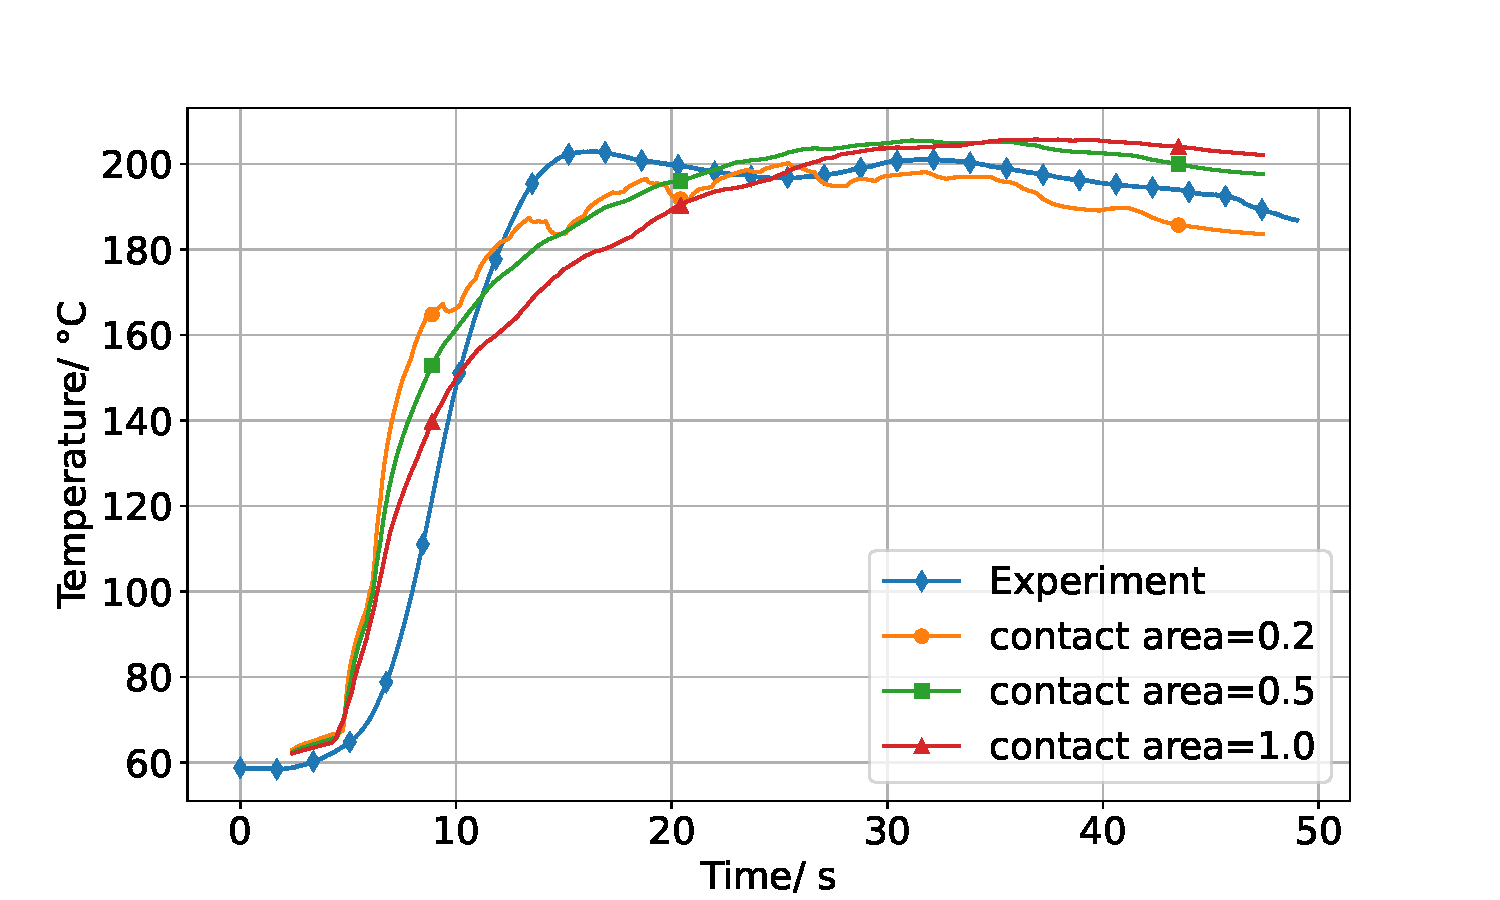
\includegraphics[width=0.8\textwidth]{chapters/zhang/graphics/T_ave_dc.pdf}
    \caption{Average temperatures with different contact areas}
    \label{fig:T_ave}
\end{figure}

As shown in Figure \ref{fig:T_ave} is the average temperature for these three cases. The maximum temperature difference is 20 $^{\circ}\text{C}$ between 20\% and 100\% contact areas. The maximum relative difference is 16.6\%. The average temperature is not sensitive to different contact areas since the total heat input is the same, while only heat dissipation is slightly different because the temperature distribution of the brake discs is uneven. Uneven temperature distribution can be proven through the comparison of the maximum temperatures.

\begin{figure}[h]
    \centering
    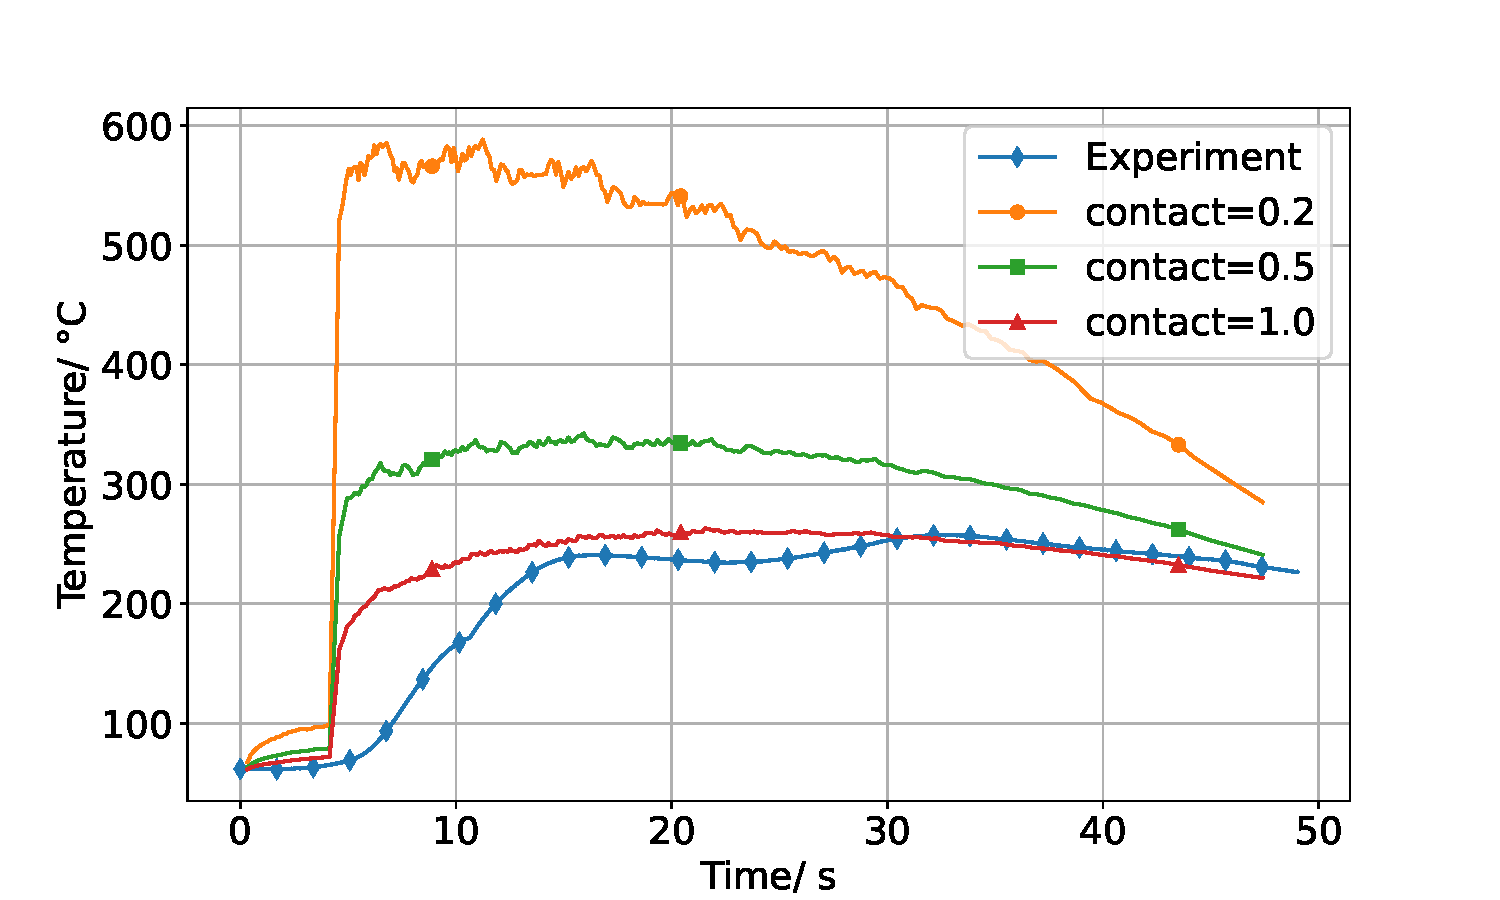
\includegraphics[width=0.8\textwidth]{chapters/zhang/graphics/T_max_dc.pdf}
    \caption{The maximum temperatures with different contact areas}
    \label{fig:T_max}
\end{figure}

Figure \ref{fig:T_max} shows the maximum temperature of the brake discs. The maximum temperature difference is more than 300 $^{\circ}\text{C}$, and the relative difference can reach 160\%. Small contact areas induce higher local temperatures since contact pressure is significantly increased and all friction heat is loaded on limited surfaces.

More advanced research can be conducted based on this FEM model, including sensitivity analysis of railway brake disc temperature development. In the future, the following need to be considered to build a more realistic model to investigate different brake designs:

\begin{enumerate}
\item Coupling elastic equations to get deformation details of the brake pads.
\item Considering more nonlinear parameters, like a variable coefficient of friction, and temperature-dependent material properties.
\end{enumerate}


\section*{Conclusion}
This study investigates the influence of contact area on the temperature of railway brake discs. A FEM model in FEniCSx is built and validated. The following conclusions can be drawn:
\begin{enumerate}
\item The contact area does not influence average temperature significantly while a small contact area induces a higher maximum temperature.
\item FEM based research on thermal analysis of brake systems should model real contact areas between brake pads and discs to get an accurate temperature distribution.
\end{enumerate}


\begin{acknowledgement}
This work is sponsored by the KTH Railway Group, China Scholarship Council and CRRC ZELC. Thanks to the experimental support of Fei Gao, Junying Yang at Dalian Jiaotong University. The help of Jørgen S. Dokken from the FEniCSx community and Jing Gong from Kungliga Tekniska Högskolans PDC support are especially acknowledged. Thanks to the National Academic Infrastructure for Supercomputing in Sweden for providing computer resources.        
\end{acknowledgement}

\bibliographystyle{spbasic}
% Write the full path of your bibfile relative to book.tex

\bibliography{chapters/zhang/bibliography.bib}



% Write the full path to the location of the graphics relative to book.tex
\graphicspath{{chapters/parsons/graphics/}}

\title{Function scaling and adaptive boundary condition throttling for
  convergence control in highly nonlinear Poisson--Boltzmann
  electrolyte models.}
\titlerunning{Function Scaling and Adaptive Convergence Throttling}

\author{D.~F.~Parsons, M.~Farci,  A.~Grigoras, Dagmawi Tadesse}
\authorrunning{Parsons et al.}

\institute{D.~F.~Parsons \email{drew.parsons@unica.it}
  \and M.~Farci \and A.~Grigoras
  \at University of Cagliari,
Department of Chemical and Geological Sciences \& CSGI,
Cittadella Universitaria, S.S. 554 bivio Sestu,
09042 Monserrato (CA), Italy
\and Dagmawi Tadesse
\at Murdoch University,
Discipline of Physics, Chemistry and Mathematics, 90 South St, Murdoch 6150, West Australia
}

\maketitle

\abstract{ The nonlinear Poisson--Boltzmann model of electrolyte
  solutions combines the Poisson equation for electrostatic potentials
  with a Boltzmann equilibrium of mobile ion concentrations. The
  Boltzmann equation $c = c_0 \exp[-e\psi/kT]$ is highly
  nonlinear once the electrostatic potential exceeds several thermal
  energy ($kT$) units (i.e.\ when $\psi>0.1$ V). This introduces two
  related numerical challenges. Firstly, suitable convergence conditions
  for the concentration functions become sensitive to the
  boundary potential. Secondly a controlled initial guess must be
  provided must be provided to avoid the FEM calculation diverging to
  NaN. We resolve the first challenge by logarithmic scaling of the
  concentration function, as suggested by the exponential nature of
  the Boltzmann equation.  We find a nontrivial complex logarithmic
  form (``log-zero scaling'') is required in order to allow for the near-zero concentrations
  of coions in a classical point-charge model.   But a better model is obtained by
  allowing for other nonelectrostatic molecular interactions, in
  particular steric forces due to finite ion sizes. The second challenge is resolved  with an adaptive
  throttling algorithm that throttles large values of
  boundary conditions down to the level of the linear regime, then 
  raises the throttle and applies the throttled solution as an initial guess until the
  final nonlinear solution  is iteratively  obtained.
The combination of a steric model with throttling enables
  computation of concentrated electrolytes with electrode potentials
  as high as 2000V. We provide a general derivation of the weak and
  strong forms of the modified Poisson--Boltzmann system from the
  underlying thermodynamic energy functional.} 

\section*{Introduction}

Continuum theory (mean field theory) has been an effective tool for
studying the behaviour of systems in electrolyte solutions. The
Poisson--Boltzmann (PB) model \citep{Wu2022} enables evaluation of ion
adsorption layers at surfaces together with the electric field that
surface charge and adsorbed ions generate. The PB model underpins
theory of stability of microparticle suspensions in aqueous media,
enabling modelling of particle aggregation and surface forces. The
same theory can also be applied to model electrochemical
systems, including energy storage devices, batteries or
supercapacitors. But there is a crucial difference in the two classes
of application, which has a significant impact on the numerical
stability of the model.  The surface potentials
of typical microparticles such as protein molecules or metal oxide
particles tends to lie in the range 5--50 mV, which is 0.2--2
$kT$ in thermal energy units (based on a thermal potential at $T=298$
K defined by $e\psi_{T} = kT$, where $e$ is the elementary charge, $k$
is Boltzmann's constant, $T$ is temperature). Electrolytic energy
storage systems, by contrast, typically operate with electrode
potentials of the order of 1--5 V, that is 1000--5000 mV, or 40--200
$kT$.  The nonlinearity of the Poisson--Boltzmann model is highly
sensitive to energies exceeding one $kT$ unit, requiring particular
algorithms to enable numerical nonlinear convergence.  Our goal is to
set up the calculation to solve successfully over a broad range of
electrode potentials without requiring manual readjustment of
convergence parameters.  We identify two main steps, implemented via
finite element methods using FEniCSx \citep{baratta2023dolfinx}: log-scaling of
ion concentration functions, and adaptive throttling of boundary
conditions.

For context we first present a summary of the physics and
derive the
weak and strong formulations defining the Poisson--Boltzmann model from
the underlying thermodynamic energy functional. The derivation
is general, allowing for a spatially varying permittivity, although we
employ a dielectric constant in calculations here. The derivation
allows for nonelectrostatic interactions of the electrolyte, in
particular steric forces due to finite ion size effects.  
In order to focus on the numerical algorithms, we omit redox
phenomena (including electrolysis of water) which would occur in real
systems at  high electrode potentials.

\section{Weak formulation of the Poisson--Boltzmann model}

The energy functional for an electrolyte solution, determined by
electrostatic potential $\psi(x)$ and ion concentration profiles
$c_i(x)$, may be composed from various fundamental energy
contributions as
\begin{equation}
    \Omega[\psi, c_i] = \Omega_{el} + \Omega_{en} +  \Omega_{ex}.
\end{equation}
$\Omega_{el}$ describes the direct energy of the electrostatic field generated by the electric charge of ions and surfaces \citep{Jackson_Classical_Electrodynamics},
\begin{equation}
  \Omega_{el}  =\frac{1}{2} \int_{V}D \cdot E dx
  = -\frac{1}{2} \int_{V}D \cdot E dx + \sum_i \int_V z_i e c_i(x) \psi(x) dx
  + \int_{S} \sigma(s) \psi(s) ds,
\end{equation}
where $E$ is the electric field, $E=-\nabla\psi$, and $D$ is the
electric displacement $D=\varepsilon_0
\varepsilon(x)E$. $\varepsilon_0$ is the permittivity of the vacuum,
and $\varepsilon(x)$ is the (spatially varying) relative
permittivity. $z_i$ is the valency of ion $i$.  $\sigma(s)$ is the
surface charge density on boundary $S$. Here $V$ refers to the domain
(volume) of the system in space.

$\Omega_{en}$ describes the ideal entropic energy of ions, treated as ideal (noninteracting) particles \citep{GrayStiles2018,DagmawiParsons2024},
\begin{equation}
    \Omega_{en} = kT \sum_{i} \int_{V} \left[ c_i(x) \ln \left(\frac{c_i(x)}{c_{i\infty}} \right) - c_{i}(x) + c_{i\infty} \right] dx,
\end{equation}
where $c_{i\infty}$ is the bulk concentration of ions. As a point of
physics, it is important to note that the use of a fixed bulk
concentration means the system is controlled by the chemical potential
of ions, with a variable number of ions in the domain $V$ of interest.
That is, the thermodynamic potential is a grand potential, not a
(Helmholtz) free energy, and for that reason we write the energy as $\Omega$ rather
than $F$. A free energy formulation (with fixed number of ions) would
require use of a thermal de Broglie wavelength instead of
$c_{i\infty}$ \citep{GrayStiles2018}.


$\Omega_{el} + \Omega_{en}$ alone construct the conventional
Poisson--Boltzmann model. The term $\Omega_{ex}$ represents extra
contributions to the total energy functional that describe other
relevant physics, such as pH-dependent charge regulation
\citep{ParsonsSalis2019}, specific ion interactions
\citep{ParsonsCarucciSalis2022}, or steric forces due to finite ion
size \citep{LopezGarciaHornoGrosse2018}. We consider the latter in this
work.

The Poisson--Boltzmann model describes the system in equilibrium,
obtained by minimising the total grand potential with variation
$\delta\Omega=0$ with respect to $\psi$ and $c_i$. Variation with
respect to $\psi$ (with test function $p \equiv \delta \psi$) leads to a weak formulation
for the Poisson equation
\begin{equation}
    0 = -\int_{V} \varepsilon_{0}\varepsilon(x) (\nabla\psi,\nabla p) dx + \sum_{i}z_i e \int_{V} c_{i}(x) p dx + \int_{S_{N}} \sigma(s) p ds
    \label{weak_Poisson}
\end{equation}
for all test functions $p$ in the relevant function space (vanishing
on the Dirichet boundary subdomain $S_{D} \subset S$).  A Dirichlet boundary
condition $\psi(x)=\psi_{0}$ for $x \in S_{D}$ may be applied to set a defined potential,
for instance the potential of an  electrode controlled by a
potentiostat. For other boundary subdomains $S_{N} = S \setminus
S_{D}$, a Neumann boundary condition may be set via the surface
charge density $\sigma$ in the surface term, applying Gauss' Law at
the external boundary,\footnote{at an internal boundary, $\sigma=D^{\text{out}}_{\perp}-D^{\text{in}}_{\perp}$}
\begin{equation}
  \sigma = -D_{\perp} = (n, \varepsilon_{0}\varepsilon\nabla \psi),
  \label{surface_charge_gauss}
\end{equation}
where $D_{\perp}$ is the transverse component of the electric
displacement vector $D$ at the boundary, or, equivalently, $n$ is the
outward normal vector at the boundary. Eq.~\eqref{surface_charge_gauss}
is valid across the entire  external surface $S$, but sets a Neumann
boundary condition when applied to the surface subdomain
$S_{N}$ in Eq.~\eqref{weak_Poisson}. Applied at $S_{D}$, it provides an
evaluation of the surface charge density generated at Dirichlet surfaces.
 After additional
integration by parts, the weak formulation Eq.~\eqref{weak_Poisson} leads to the strong
formulation of the electrostatic Poisson equation,
$\nabla\cdot D = \sum_i z_i e c_{i}(x)$.

The variation of $\Omega$ with
respect to each ion concentration profile $c_i$ (in turn, with test
functions $b_i\equiv \delta c_i$), assuming linear variations such that
$\ln(1+b_i/c_i)\approx b_i/c_i$, leads to the weak formulation of Boltzmann's
equation,
\begin{equation}
    0 = \int_{V} \left[ e z_i \psi(x)
    + kT \ln\left(\frac{c_i(x)}{c_{i\infty}}\right)
  \right] b_i dx,
    \label{weak_Boltzmann}
\end{equation}
for all test functions $b_i$. The strong form of the classical
Boltzmann equation can then be obtained, $c_i(x)=c_{i\infty}\exp(-z_i
e \psi(x)/kT)$.  The Boltzmann equation is implicitly controlled by
the bulk concentrations $c_{i\infty}$, and an explicit boundary condition
for the concentration functions is not needed.

\subsection{Nonelectrostatic interactions: Steric model with  finite ion size}

 In the classical point-charge Poisson--Boltzmann model, the
ion concentrations $c_i$ are determined completely by the
electrostatic potential with the Boltzmann equation in closed form,
such that
only the Poisson equation would need to be solved directly. However, the
physical problem with the classical model is evident in electrochemical
systems with electrode potential 1 V. A one volt potential is
equivalent to a thermal energy of $40 kT$ (at room temperature), for which the conventional
Boltzmann factor for a counterion is
$\exp(40)\approx 2.3 \times 10^{17}$.  That is, the surface counterion
concentration of a 1M electrolyte would exceed $10^{17}$ mol/L, which
is clearly unphysical.  We return the model back to physical
relevance by adding an extra steric energy term $\Omega_{ex}$ with
corresponding excess chemical potential per ion $\mu_{i}^{ex}$, for
which the modified Boltzmann equation is
\begin{equation}
    c_i(x)=c_{i\infty}\exp\left[(-(z_i e \psi(x) + \mu_i^{ex}(x)-\mu_{i\infty}^{ex})/kT\right].
    \label{general_Boltzmann}
\end{equation}
This corresponds to a total chemical potential $\mu_i(x)$ of each ion,
defined by
\begin{eqnarray}
  \mu_i(x) &=& \mu_{i}^{\textrm{entropic}} +  \mu_{i}^{\textrm{electrostatic}} +
               \mu_{i}^{ex} \\
{} &  =&\mu_{i\infty} + kT \ln(c_i(x)/c_{i\infty})
         + ez_i \psi(x) + \mu_i^{ex}(x)-\mu_{i\infty}^{ex}.
         \label{chem_pot}
\end{eqnarray}
$\mu_{i\infty}$ refers to the (fixed) excess chemical potential of the
ion in bulk solution, defined relative to an ideal unit
reference solution by $\mu_{i\infty} = kT\ln c_{i\infty} + \mu_{i\infty}^{ex}$.
The steric model we employ is the Carnahan--Starling (CS) model
\citep{CarnahanStarling1969} with a contribution to the grand potential
% for future reference, the CS model (both energy and chemical
% potential)  can be considered as Padé approximations
% i.e. rational  polynomials functions
% which give good convergence when used in the Homotopy Series Method
% thus tells us Liao
\begin{equation}
    \Omega_{ex} = \sum_{i} \int_{V} c_{i}(x) \left[ kT
    \frac{4\phi - 3\phi^2}{(1-\phi)^2}
    -  \mu_{i\infty}^{ex}
  \right]dx
  \label{CS_energy_functional}
\end{equation}
and weak formulation
\begin{equation}
    0 = \int_{V} (\mu_i^{ex}-\mu_{i\infty}^{ex}) b_i \, dx
    \label{weak_CS}
\end{equation}
for all $b_i$, which is added to Eq.~\eqref{weak_Boltzmann}, the weak
formulation for the Boltzmann equation, together generating the strong
formulation of the modified Boltzmann
equation,  Eq.~\eqref{general_Boltzmann}.  Here the excess chemical potential
per ion for the Carnahan--Starling (CS) model, corresponding to the energy
functional Eq.~\eqref{CS_energy_functional}, is
\begin{equation}
    \mu_{i}^{ex} = kT \frac{\phi(8-9\phi+3\phi^2)}{(1-\phi)^3}.
    \label{chem_pot_CS}
\end{equation}
$\phi$ is the \emph{total} ion volume fraction defined by
$\phi=\sum_i c_i v_i$ where $v_i$ is the intrinsic molar volume per
ion $i$. Hence the CS excess chemical potential is defined identically
for all ions. To derive the weak formulation in Eq.~\eqref{weak_CS}, we
applied an homogenised component approximation that assigns common
volumes at the point of introducing the variation  $\delta c_i$ (i.e.\
the test function $b_i$), such that $\delta\phi=v_j \delta c_i$ rather 
than $v_i \delta c_i$. This approximation is required since the CS
model was formulated for single component systems. The more complex
multicomponent BMCSL model would enable ion specific chemical
potentials \citep{MansooriCarnahanStarlingLeland1971}, removing the
need for this approximation.  $\phi_{\infty}$, $\mu_{i\infty}^{ex}$
are the bulk total volume fraction and excess chemical potential
defined by bulk concentrations $c_{i\infty}$. With this term, the
Boltzmann equation Eq.~\eqref{general_Boltzmann} becomes transcendental in $c_i$, precluding a closed
expression that would determine ion concentrations. Concentration functions must therefore be
explicitly solved  numerically alongside potential $\psi$. In this
paper we address strategies for managing the strong nonlinearity in
the system introduced by this term when large values of the
potential are present. Note that $c_i$ must also be solved explicitly in the case
of time-dependent nonequilibrium Poisson-Nernst-Planck (drift-diffusion) systems \citep{LopezGarciaHornoGrosse2018} where
ion concentrations are not in equilibrium and determined by a
continuity equation rather than a Boltzmann equation.

One last point on the weak formulation of the Boltzmann equation. The variational
derivation of these weak formulations from the energy functionals,
Eq.~\eqref{weak_Boltzmann} and Eq.~\eqref{weak_CS}, presents them in terms of the
chemical potential of the ions, Eq.~\eqref{chem_pot}, not the concentration directly. That
is, fundamentally the strong form of the Boltzmann equation is simply $\mu_i(x) =
\mu_{i\infty}$, the condition of equal chemical potential at all
points in the domain in equilibrium with an external bulk bath.
The Boltzmann
equation in terms of 
concentration, Eq.~\eqref{general_Boltzmann}, is then simply a rearrangement of
the strong equation for chemical potential. Chemists are in the
habit of using the Boltzmann equation in concentration form rather
than chemical potential, in practice our implementation in code applies the weak
form of the Boltzmann equation via concentrations, as
\begin{equation}
0 =   \int_V \left[ c_i(x) - c_{i\infty}
    e^{-\left(z_i e \psi(x) +
      \mu_i^{ex}(x)-\mu_{i\infty}^{ex}\right)/kT} \right] b_i
dx 
\label{weak_Boltzmann_conc}
\end{equation}
for all test functions $b_i$, rather than applying it via the chemical
potential components in Eq.~\eqref{weak_Boltzmann}
+Eq.~\eqref{weak_CS}. Because the concentration functions $c_i(x)$ being
solved are the same, this change in weak form should not affect
residuals.  These alternative weak forms for the Boltzmann
equation may affect efficiency, perhaps by changing the condition number
of the matrices involved. Our
testing found the chemical potential formulation to be less stable than the
concentration formulation, failing to converge with an 1V electrode
potential, where the latter weak form achieves successful convergence
with the log-zero concentration scaling described below.

\section{Numerical convergence}

\subsection{Graded mesh}
Solution of the nonlinear Poisson-Boltmann model requires a finer mesh in the  region
close to an electrode boundary, rendering solutions on a uniform linear mesh  impractical at electrode
potentials greater than 0.1V.  The general exponential nature of the potential,
$\psi(x) \sim \psi_{0} \exp(-\kappa x)$, suggests logarithmic spacing of
mesh may be suitable.
A graded mesh spacing can be achieved with a geometric sequence of
mesh points  to obtain finer spacing for the points closer to the boundary.
For the simple planar geometry of a flat electrode located at $x=0$,
where $x$ is the perpendicular distance from the boundary,
we take a uniformly spaced set of $s \in [0,1]$  (e.g. $s=x'/L$ for an
initially uniformly spaced $x'\in [0,L]$) , and obtain a sufficiently
well graded mesh with
\begin{equation}
  x = s^3 L.
\end{equation}
Symmetry renders the system of the flat electrode essentially one-dimensional along the
perpendicular $x$-coordinate, although the calculation can be performed in a 2D
or 3D geometry. Whether in 1D, 2D, or 3D, the same graded mesh can be
applied  along the  $x$-direction.
For more complex non-planar geometries, adaptive mesh refinement would
be suitable, likely controlled by the magnitude of the gradient of the
electrostatic potential (i.e.\ the electric field) or by concentration
gradients.

The Debye length (electrostatic screening length) of the electrolyte
provides a natural reference for the units of $L$. The Debye length is
the  decay length of the exponential decaying profile of the potential $\psi(x)$
found far from the electrode where its magnitude has fallen below 25
mV. The distance to zero potential (bulk solution) may be taken as
$L=10$--30 Debye lengths, depending on one's tolerance for
``zero''. The Debye length itself could be taken as the length unit
for $L$. But typical Debye lengths lie in the nanoscale, ranging from 0.5 nm for
sea water (0.5M salt), to 1000 nm for pure water (due to {H}$^{+}$ and
{OH}$^{-}$ from dissociated water). We use nm as the units for $L$ to facilitate
comparison of length scales in different systems, setting $L$ as
approximately 30 Debye lengths (in nm) to reach bulk solution. At
higher potentials above
100V we amplify that value of $L$ by a factor 2 to allow for the formation of a steric counterion adsorption
layer before the decay region is reached \cite{DagmawiParsons2022}.

\subsection{Solver description}
We constructed a finite element implementation of the weak
formulation (Eq.~\eqref{weak_Poisson} and \eqref{weak_Boltzmann_conc}) in
FEniCSx \citep{baratta2023dolfinx}, using continuous
Lagrange elements with polynomial order 2 (linear elements with order
1 may also be used).  The electrolyte solution
is taken as NaCl with bulk concentration 1 mol/L.  To illustrate
general issues of nonlinear convergence, we calculate the
electrostatic and ion concentration profiles of ion adsorbed at a
single flat electrode surface along the direction perpendicular to the
surface, with the electrode boundary at $x=0$.  The electrode
potential is controlled (Dirichlet boundary condition), and bulk
solution represented by a zero Neumann condition (``zero net charge'', ``zero electric
field'') at  a distance of 10 nm (~30 Debye lengths for the 1M
electrolyte). Nonlinear solutions are computed using FEniCSx's
\texttt{NonlinearProblem} with a standard Newton solver. Convergence criterion
is set to DOLFINx's default ``incremental'' method with absolute
tolerance $10^{-5}$.
We set PETSc options \citep{PETSc_manual,petsc4py_2011} configuring the solver to use the LU direct
solver provided by MUMPS \citep{MUMPS_2001,MUMPS_2019}, with the PETSc Krylov type set to apply the
preconditioner only once (\verb|ksp_type=preonly|, \verb|pc_type=lu|,  \verb|pc_factor_mat_solver_type=mumps|).
By contrast, for instance, a
conjugate gradient solver (\verb|ksp_type=cg|, \verb|pc_type=gamg|)
generates a spurious oscillatory electrostatic potential profile with electrode
potentials higher than 0.1 V.

In our implementation we have adopted nm for the length scale of the
mesh ($x$). The physical units for real  electrostatic potential
$\psi(x)$ and concentration functions  $c_{i}(x)$, are Volts and M
(mol/L), respectively. However in computations we used units for the
potential and concentration functions scaled to unity, described next.

\subsection{Function scaling}
The electrostatic potential $\psi(x)$ is handled with trivial
scaling, solving $P(x)=\psi(x)/\psi_0$, where $\psi_0$ is the
electrode potential.
But we must take more care scaling the concentration functions
$c_i(x)$.
We already noted that the counterion concentration becomes unphysically
large in the conventional point-charge model due to nonlinear
exponentiation of  electrostatic potentials exceeding 0.1--0.2 V in
the Boltzmann equation. Trivial scaling may be introduced by solving
the concentration function scaled against the bulk concentration. But
 the nonlinear catastrophe is reached
numerically above 0.5 V. Already at 0.6 V, the conventional
calculation with simple scaling is unable to reduce the residual below
the required convergence criterion  $10^{-5}$. While it would be possible to relax the
convergence tolerance to obtain a reasonable solution, our aim is to
obtain a robust general solver not requiring close manipulation of
convergence criteria. For instance,  modelling the
cyclic voltammetry curve of an electrode may require calculations
over a potential window as wide as $-5$ to 5 V.

The challenge arises due to the extreme magnitudes of the counterion
concentration at the electrode surface. The weak formulation for the
Boltzmann equation in Eq.~\eqref{weak_Boltzmann} suggests a solution:
solve for the concentration function in log-form
\begin{equation}
C_{i}(x) = \ln[ c_{i}(x) / c_{i\infty}]
\label{log_scaling}
\end{equation}
rather than the physical concentration function $c_{i}(x)$ directly. Log
scaling extends the solvability of the conventional point-charge Poisson--Boltzmann
model up to electrode potentials as high as 1.5 V. Solutions for the
electrostatic potential and counterion concentration profile are shown
in Fig.~\ref{fig_classical_PB}. Shown on a log scale, strong
nonlinearity in the PB system becomes apparent in the bend in the
electrostatic potential (Fig.~\ref{fig_classical_PB}a) close to the
surface ($x<2$\AA) for electrode potentials $> 0.2$ V.

\begin{figure}
\centering
(a)
\includegraphics[width=0.45\linewidth]{counterion_potential.eps}
(b)
\includegraphics[width=0.45\linewidth]{counterion_logzero.eps}
\caption{\label{fig_classical_PB}Solutions to the classical point
  charge Poisson--Boltzmann model of 1M NaCl electrolyte solution,
  shown as profiles along $x$, the perpendicular distance from an
  electrode surface (a) Electrostatic potential. (b) Counterion
  ({Cl}$^{-}$) concentration. }
\end{figure}

At still higher potentials the stability of simple log scaling with
respect to the coion must be considered. The coion, with same charge
as the electrostatic potential, is repelled from the electrode surface,
resulting in coion concentrations trending towards zero near the electrode. At
sufficiently high potentials this generates values in the log-scaled
function that tend towards $-\infty$, which destabilises the numerical
solution (residuals become infinite). We therefore introduce a more complex log-scaling function
\begin{equation}
Z_i(x) = \ln\left[c_i(x)/c_{i\infty}+1\right]/\ln 2 - 1
\label{log_zero}
\end{equation}
which keeps the scaled coion function constrained between -1 and 0
rather than $-\infty$ and 0. Since this scaling function addresses the
near-zero concentration of the coion, we call it ``log-zero'' scaling.

\subsection{Throttling algorithm}

Log-zero scaling of concentration functions facilitates a successful numerical solution to
the conventional Poisson--Boltzmann at electrode potentials
exceeding 1V. Nevertheless Fig.~\ref{fig_classical_PB}b demonstrates the
point charge catastrophe of the conventional model, with counterion
concentrations exceeding $10^{5}$ mol/L at the electrode
surface. Moreover, for general electrochemical applications it would
be desirable to be capable of obtaining solutions for electrode
potentials higher than 1.5V. To deal with the physical problem, we
introduce finite ion sizes with a steric force provided by the
Carnahan--Starling model, Eq.~\eqref{chem_pot_CS} (weak form
Eq.~\eqref{weak_CS}).  We apply ion volumes
$v_{{Na}}=1.24 \textrm{\AA}^{3}$ per {Na}$^{+}$ ion,
$v_{{Cl}}=35.9 \textrm{\AA}^{3}$ per {Cl}$^{-}$ ion (these are
quantum mechanical volumes of the electron clouds \citep{ParsonsNinham2009}).

The additional nonlinearity introduced by the Carnahan--Starling model,
where the chemical potential depends on the concentrations being
calculated, introduces a new challenge. The default nonlinear solver
in FEniCSx assumes zero as an initial guess for the functions being
solved. But under the nonlinear conditions (with electrode potential
$>0.2$ V) where the Carnahan--Starling steric force is required, the
zero initial guess leads quickly to a diverging solution with infinite
or NaN
residual. And yet a stable solution is accessible at lower values of
the boundary condition. We nudge the solver to a stable solution by
applying a throttling algorithm: reduce the boundary condition to a
small value for which a solution can be obtained, then incrementally
increase the boundary value back towards the target value, using the
previous found solution as an initial guess for the next
iteration. The approach is known to mathematicians as a homotopy
method \citep{homotopy_analysis_Liao2012}
or numerical continuation method \citep{allgower1990numerical},
with our throttle serving as a homotopy parameter applied to boundary
conditions.  A flowchart for the algorithm is shown in
Fig.~\ref{fig:throttling_algorithm}.

\begin{figure}
\centering
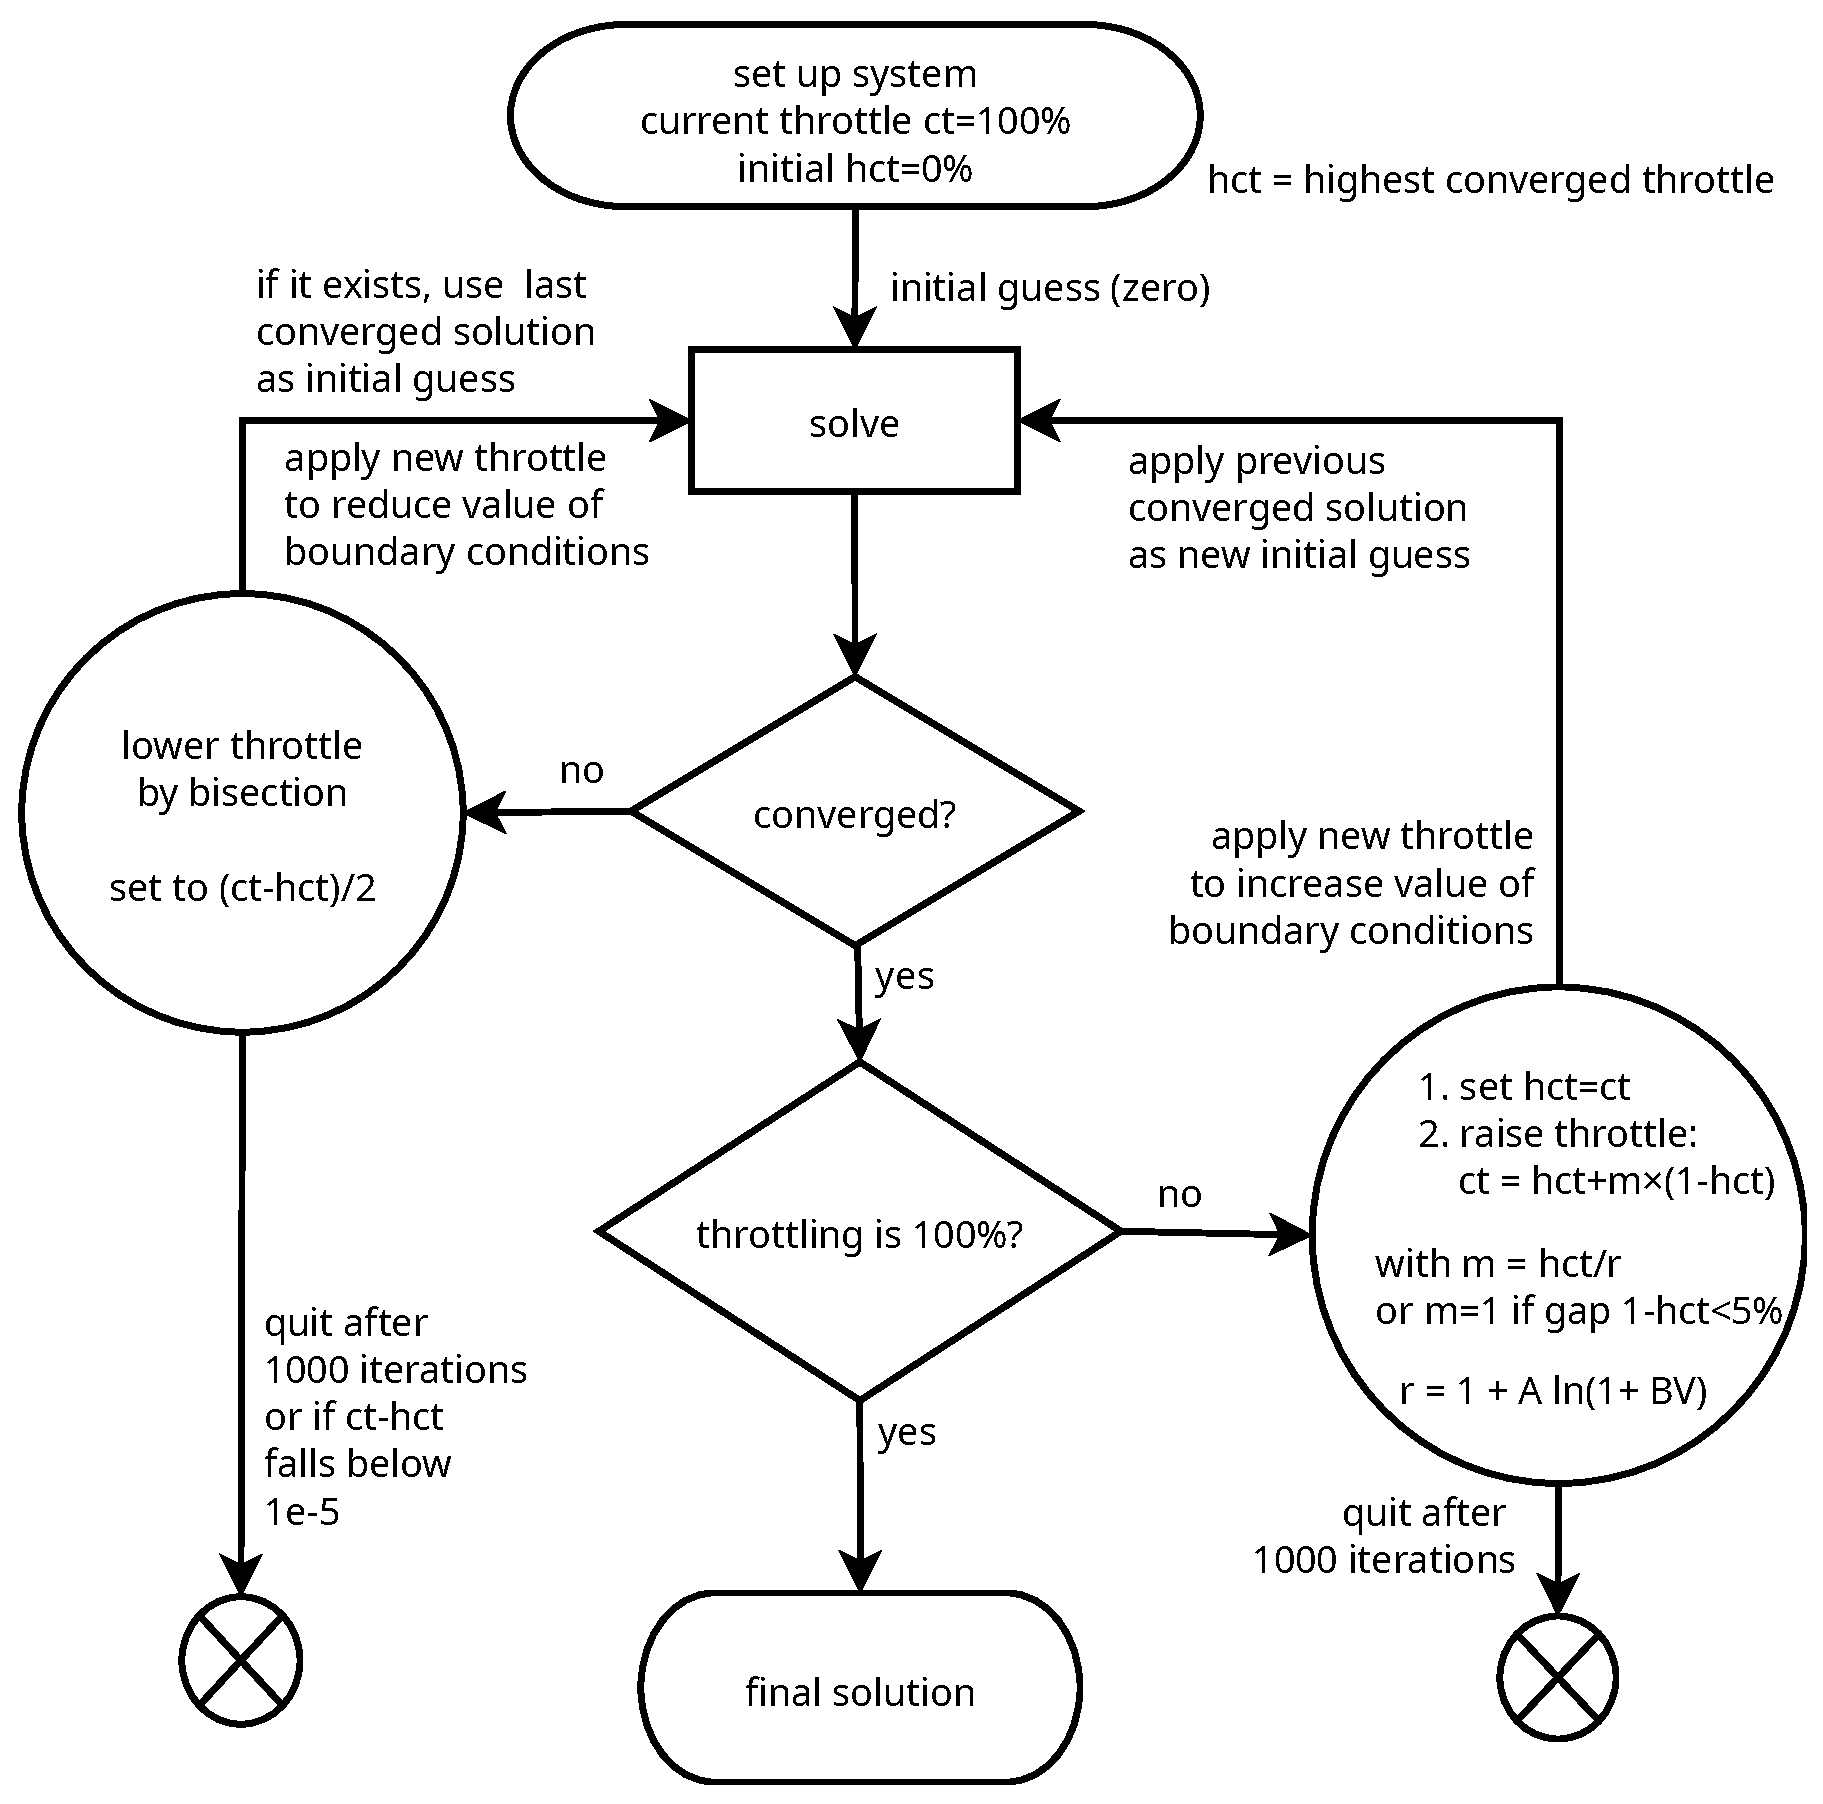
\includegraphics[width=1.1\linewidth]{throttling4.eps}
\caption{Flowchart for the throttling algorithm. }
\label{fig:throttling_algorithm}
\end{figure}

The throttle is a multiplier
applied to the magnitude of the boundary conditions.
If the solver fails to converge, then reduce the throttle downwards by
bisection between the current failed value (``current throttle'', ct) and the highest converged
throttle (hct, initially 0). Once the boundary
condition is throttled low enough to generate a converged solution,
update the hct and raise
the throttle upwards by an amount $u$, closing the gap towards 100\% (set the throttle
to 100\% if the procedure would exceed it).  The value of $u$
must find a balance between reaching 100\% throttle in as few
iterations as possible (don't make $u$ too small), while not collapsing back to non-converging
conditions when raising the throttle (don't make $u$ too
large). Empirically we find that when the hct is small, the rise rate
must also be small to obtain the next converged iteration. Once hct is
large, the rise rate may be proportionally larger. We therefore
propose a rise step $u=m\times (1- \mathrm{hct})$, such that the next
throttle applied after a converged iteration is
\begin{equation}
  \mathrm{ct [new]} = \mathrm{hct} + m (1-\mathrm{hct})
\end{equation}
with
\begin{equation}
  m=
  \begin{dcases}
    \frac{\mathrm{hct}}{r} & \\
    1 & \text{if } 1-\mathrm{hct} < 5\%
  \end{dcases}.
\end{equation}
This produces a quadratically accelerating rise rate,  and attempts a
direct jump to 100\% once the remaining gap is less than 5\%.  It is likely
that our formulation, quadratic in hct, approximates a more 
optimal exponential (or
sigmoidal) rise rate.

\subsubsection{Optimal throttling}
An example of
the  throttle rate against number of iterations is shown in
Fig.~\ref{fig:throttle_rate} for 1V and 10V boundaries with different
choices of fixed values of the rise rate multiplier $r$. A best value of $r$ can be identified
for each voltage, minimising the number of iterations required,
e.g. $r=2$ for 1V, and $r=3$ for 10V. A
value of $r$ larger than the best value means the rise step is
smaller, such that convergence is smooth, but requires more
iterations. A lower value of $r$ means the rise step is too large,
overstepping and resulting in a nonconverging iteration, such that
more iterations are required to fall back to a converging throttle rate.

\begin{figure}
\centering
(a)
\includegraphics[width=0.45\linewidth]{test_1V.eps}
(b)
\includegraphics[width=0.45\linewidth]{test_10V.eps}
\caption{Attempted throttle rate vs iteration number, for (a) 1V and
  (b) 10V  boundaries with fixed rise rate multipliers $r=1,2,3$ and
  4. Solving the steric model with log-zero scaling.
}
\label{fig:throttle_rate}
\end{figure}

The best-performing fixed values of $r$  for potentials up to 100V are shown
in  Fig.~\ref{fig:best_throttle_rate}.  We observe a similar trend in 1D calculations with
trivial and log-zero function scaling  (the
differences may not be significant since only integer values of $r$ up
to 10 were tested). \textit{A priori} we have no reason to expect the
optimal value of $r$ to be universal, and might expect it to vary with
conditions such as electrolyte concentration or
dimensionality. However, we plot the best $r$ for trivial
scaling over  a wide range of concentrations (1D calculations), and
also 2D and 3D calculations of the flat electrode (at 1M
concentration). In all cases the best $r(V)$  essentially follows the
same curve, with a small deviation seen only at 1--2V, which may be attributed simply to the
integer resolution of the simulation.  The time per iteration varies with system conditions and
dimensionality. But the optimal $r(V)$ for minimising the number of
iterations remains the same. The optimal $r(V)$ may be considered universal.



\begin{figure}
\centering
\includegraphics[width=0.8\linewidth]{best_r_vs_V.eps}
\caption{Best fixed rate multiplier $r$ for each voltage, giving lowest
  number of throttling iterations. The steric model is solved with both
  trivial (black) and log-zero (orange dash) concentration scaling (1D calculation at 1M
  electrolyte concentration).
  We also show best $r$ for 1D calculations with trivial scaling over a range of
  concentrations (blue starpoints);
  and 2D and 3D calculations (black box points) of a flat electrode at
  1M concentration. The solid purple line marks the model $r(V) = 1 +
  3.78 \ln(1 + 0.102 V)$ fitted to trivial scaling data. Grey lines
  mark uncertainty bounds of one standard deviation in the fitted parameters.
}
\label{fig:best_throttle_rate}
\end{figure}


\subsubsection{Adaptive throttle rate}
The trend in best-performing $r$ shown in Fig.~\ref{fig:best_throttle_rate} suggests that an
optimal multiplier follows
$r \propto \ln V$, indicating that $r$ 
may be tuned adaptively to provide the maximum possible rise rate (smallest
possible $r$) that minimises the number of unsuccessful non-converged
attempts for the given boundary condition.  A milder
rise rate (larger $r$) is required at larger surface potentials.
Allowing for a finite value of $r$ when $V \rightarrow 0$, we propose
an adaptive definition of $r$,
\begin{equation}
  r(V) = 1 + A \ln(1 + B V).
  \label{adaptive_r}
\end{equation}
This model imposes the limit $r \rightarrow 1$ as $V \rightarrow 0$.
In principle an optimal low-voltage multiplier might allow $r<1$, if
$r>$hct, but the limit 1 is simpler, avoiding the need to 
compare against hct.  Fitting against best $r$ for trivial scaling
obtains $A=3.78 \pm 0.36$, $B=0.102 \pm 0.020 \textrm{ V}^{-1}$.
The uncertainties here have been determined from the covariance matrix
generating by the fitting procedure implemented in the
\verb|curve_fit| function provided by the optimize module in scipy
\cite{VugrinSwilerRobertsStuckyMackSullivan2007}. 
 Best $r$ for log-zero scaling is similar. One could separately fit
 parameters for log-zero scaling (to get
 $A=1.3\pm 0.2$, $B=0.7 \pm 0.5 \textrm{ V}^{-1}$).
 Nevertheless,  Fig.~\ref{fig:best_throttle_rate} shows that the
 log-zero data points lie only one standard deviation below the trivial
scaling fit. Statistically there is no significant difference in the
best-$r$ values for trivial and log-zero scaling.

We emphasise that the value of $V$ used in the adaptive $r$ formula, Eq.~\eqref{adaptive_r},
must be the target boundary condition (the final electrode voltage),
not the throttled boundary condition at the given iteration.  If a throttled $V$ were
applied, $r$ would be small when the boundary condition is strongly
throttled, resulting in large rise steps that cause convergence
failure when the  target voltage is large.


Table.~\ref{tab:convergence} shows  the number of iterations required
to converge with various boundary conditions for the different
concentration scaling functions, in both the point charge model and the
steric model, and applying adaptive
$r(V)=1+3.78\ln(1+0.102V)$ for 1D meshes with 30 cells. For the point charge model, trivial scaling only
permits calculation up to 0.7V. Log scaling reaches 0.8V, log-zero
scaling reaches 1V (1.5V may be reached with a finer mesh).

\begin{table}
  \centering
  \begin{tabular}{c|ccc|ccc}
pot(V)  & \multicolumn{3}{c|}{Point charge} & \multicolumn{3}{c}{Steric}    \\
        & trivial & log & log-zero & trivial & log & log-zero \\ \hline
%%%%%%%%%%%%%%%%%%%%%%%%%%%%%%%%%%%%%%%%%%%%%%%%%%%%%%%%%%%%%%%%%%%%%%
%%                                                                  %%
%%  This is a LaTeX2e table fragment exported from Gnumeric.        %%
%%                                                                  %%
%%%%%%%%%%%%%%%%%%%%%%%%%%%%%%%%%%%%%%%%%%%%%%%%%%%%%%%%%%%%%%%%%%%%%%
%NaCl 1M	&	&	&	&	&	&\\
%	&pot(x)/surf\_pot + non linear geometry 	&	&	&	&	&\\
%	&Steric OFF	&Steric OFF + log	&Steric OFF + log\_zero	&Steric ON	&Steric ON + log	&Steric ON + log\_zero\\
%Surface Potential [V]	&Throttle attemps	&	&	&	&	&\\
0.1	&1	&1	&1	&1	&1	&1\\
0.5	&1	&1	&1	&1	&11	&9\\
0.7	&6	&1	&1	&1	&11	&11\\
0.8	&S	&10	&6	&6	&11	&11\\
0.9	&	&S	&8	&1	&14	&12\\
1	&	&	&7	&1	&14	&12\\
1.1	&	&	&F	&7	&14	&14\\
1.5	&	&	&	&10	&15	&15\\
2	&	&	&	&8	&19	&16\\
5	&	&	&	&18	&27	&27\\
10	&	&	&	&27	&F	&39\\
100	&	&	&	&91	&	&114\\
%250	&	&	&	&240	&	&180\\
%375	&	&	&	&355	&	&212\\
%500	&	&	&	&419	&	&230\\
%625	&	&	&	&478	&	&321\\
%750	&	&	&	&517	&	&382\\
%875	&	&	&	&551	&	&428\\
1000	&	&	&	&439	&	&369    \\
2000	&	&	&	&S	&	&762    
  \end{tabular}
\caption{\label{tab:convergence}Number of throttling iterations
  required to  solve the Poisson--Boltzmann model of a 1M NaCl electrolyte solution
  for various electrode potentials and concentration scaling
  functions (trivial, log, or log-zero scaling), for both the classic point charge model, and the steric
  model (Carnahan--Starling) with finite ion sizes. Adaptive rise rate
  multiplier $r(V)=1+3.78\ln(1+0.102V)$, for 1D mesh with 30 cells. 
  ``F''=Failed
  (throttle step $<10^{-5}$). ``S''=Stopped at 1000 iterations.}
\end{table}


Trivial scaling is successful with the steric model up to 1000V, while simple log
scaling fails at 10V due to instability introduced by near-zero coion
concentrations.
Log-zero scaling enables calculation to 2000V
and greater, beyond the limit of trivial scaling.
The corresponding
performance plot of iterations vs voltage for the steric model
(with both trivial and log-zero scaling) is shown in Fig.~\ref{fig:convergence}.
 The steric model
naturally keeps concentrations within 
physically reasonable bounds, such that  log-zero scaling is not
required for normal electrochemical conditions. In fact
trivial scaling performs better than log-zero scaling when $V<100$V,
the region of electrochemical interest.
Performance is robust with respect to the $A$, $B$ parameters used to
determined $r(V)$, whether fitted to best-$r$ for trivial or log-zero scaling.
2D and 3D calculations generally require the same number of iterations
as 1D calculations, showing small differences only at 1--2V.
Even with log-zero scaling, computation of the interaction of
100~kV electrical transmission cables with saline water would require
such a large number of iterations that this algorithm would become impractical.

\begin{figure}
\centering
\includegraphics[width=0.8\linewidth]{num_attempts_vs_V.eps}
\caption{Number of throttling iterations,  as a function of electrode
  voltage, needed to solve the steric model with trivial and log-zero scaling.
  Uses an adaptive rise rate multiplier
  $r(V)=1+3.78\ln(1+0.102V)$ fitting to best trivial scaling (solid
  curves). 1D calculations with trivial scaling are shown in black,
  and log-zero scaling in orange. Rise rate $r(V)=1+1.3 \ln(1+0.7V)$
  (fitted for best log-zero) is also shown (dash curves) for
  comparison. 2D data points are shown with square (trivial scaling) and
  diamond (log-zero scaling) symbols. 3D data points (trivial scaling) are
  shown as blue crosses.
}
\label{fig:convergence}
\end{figure}


Sample results of the adaptive throttling algorithm for an electrode charged to
10V, with Carnahan--Starling steric forces, are shown in
Fig.~\ref{fig_results_throttling}, calculated with trivial scaling of the
concentration functions with adaptive $r$ coefficients $A=3.78$, $B=0.102 \textrm{ V}^{-1}$).
Fig.~\ref{fig_results_throttling}b shows the onset
of a steric adsorption layer \citep{DagmawiParsons2022} with counterion
concentrations constrained below a concentration cap determined by the
ion size, a cap of 46 mol/L in the case of our {Cl}$^{-}$ ion.

\begin{figure}
\centering
(a)
\includegraphics[width=0.45\linewidth]{steric_potential_10V.eps}
(b)
\includegraphics[width=0.45\linewidth]{steric_10V_counterion.eps}
\caption{\label{fig_results_throttling}Solutions to the modified
  Poisson--Boltzmann model of a 1M NaCl electrolyte solution with
  Carnahan--Starling steric forces, shown as profiles along $x$, the
  perpendicular distance from a 10V electrode surface (a) Electrostatic
  potential. (b) Counterion ({Cl}$^{-}$) concentration. }
\end{figure}

\section{Conclusion}

Modelling complex electrolyte solutions in electrochemical conditions
with electrode potentials 1V or greater requires both nontrivial
physics and nontrivial numerical algorithms.
With respect to the
physics, aside from redox chemistry and electrolysis (not considered
here), the finite sizes of ions must be taken into consideration via
steric forces. These are expressed as a steric contribution to the
chemical potential of ions and used in the underlying thermodynamic
energy functional that provides the origin of the weak and strong
formulations of the system.
In order to achieve numerical convergence, we have proposed two
steps. Firstly, we propose log-zero function scaling of
concentration functions that accounts
not only for the heightened concentrations of counterions near an
electrode, but also the near-zero concentrations of coions. Secondly,
and more importantly, we propose an adaptive throttling algorithm (a kind of homotopy
method) that reduces boundary conditions 
down to the linear regime where a solution is easily obtained, then
progressively propagates that solution by releasing the throttle
until the target boundary condition is obtained. Optimised convergence
is obtained by adaptively controlling the rise rate of the throttle factor
depending on the target boundary condition.

The combination of
log-zero scaling and throttling facilitates calculations of point
charge models up to 2V. Log-zero scaling enables
the steric model to reach electrode potentials greater than 2000V.
But for typical electrochemical applications with potentials lower than 20V,
where steric forces are needed in order to maintain the physical relevance
of the model, trivial scaling is sufficient, and faster than log-zero scaling.
The empirical parameters for optimal throttling, minimising the number of
required iterations, appear to be universal, independent of
electrolyte concentration or whether the geometry is 1D, 2D or 3D.
This might indicate a deeper structure in the algorithm that could be
revealed with further mathematical analysis. Our 1D, 2D and 3D
simulations tested the same flat electrode surface. We expect the optimal throttling
conditions will continue to apply with more complex 3D or 2D
geometries, though it may be prudent to confirm this assumption.

We illustrated the throttling algorithm using Dirichlet boundary
conditions (electrode potentials), but the  principle applies
equally to Neumann or more complex boundary conditions.

\begin{acknowledgement}
  We acknowledge the award of CINECA support under the ISCRA
  initiative, for the availability of high-performance computing
  resources and support.

  A Python script demonstrating the throttle algorithm is available on Zenodo at
\\  \url{https://doi.org/10.5281/zenodo.14829963}

\end{acknowledgement}

\bibliographystyle{spbasic}
% Write the full path of your bibfile relative to book.tex
\bibliography{chapters/parsons/bibliography.bib}




\backmatter%%%%%%%%%%%%%%%%%%%%%%%%%%%%%%%%%%%%%%%%%%%%%%%%%%%%%%%
\appendix
%%%%%%%%%%%%%%%%%%%%%% appendix.tex %%%%%%%%%%%%%%%%%%%%%%%%%%%%%%%%%
%
% sample appendix
%
% Use this file as a template for your own input.
%
%%%%%%%%%%%%%%%%%%%%%%%% Springer-Verlag %%%%%%%%%%%%%%%%%%%%%%%%%%

\chapter{Chapter Heading}
\label{introA} % Always give a unique label
% use \chaptermark{}
% to alter or adjust the chapter heading in the running head

Use the template \emph{appendix.tex} together with the document class SVMono (monograph-type books) or SVMult (edited books) to style appendix of your book.


\section{Section Heading}
\label{sec:A1}
% Always give a unique label
% and use \ref{<label>} for cross-references
% and \cite{<label>} for bibliographic references
% use \sectionmark{}
% to alter or adjust the section heading in the running head
Instead of simply listing headings of different levels we recommend to let every heading be followed by at least a short passage of text. Further on please use the \LaTeX\ automatism for all your cross-references and citations.


\subsection{Subsection Heading}
\label{sec:A2}
Instead of simply listing headings of different levels we recommend to let every heading be followed by at least a short passage of text. Further on please use the \LaTeX\ automatism for all your cross-references and citations as has already been described in Sect.~\ref{sec:A1}.

For multiline equations we recommend to use the \verb|eqnarray| environment.
\begin{eqnarray}
\vec{a}\times\vec{b}=\vec{c} \nonumber\\
\vec{a}\times\vec{b}=\vec{c}
\label{eq:A01}
\end{eqnarray}

\subsubsection{Subsubsection Heading}
Instead of simply listing headings of different levels we recommend to let every heading be followed by at least a short passage of text. Further on please use the \LaTeX\ automatism for all your cross-references and citations as has already been described in Sect.~\ref{sec:A2}.

Please note that the first line of text that follows a heading is not indented, whereas the first lines of all subsequent paragraphs are.

% For figures use
%
\begin{figure}[t]
\sidecaption[t]
% Use the relevant command for your figure-insertion program
% to insert the figure file.
% For example, with the graphicx style use
\includegraphics[scale=.65]{figure}
%
% If no graphics program available, insert a blank space i.e. use
%\picplace{5cm}{2cm} % Give the correct figure height and width in cm
%
\caption{Please write your figure caption here}
\label{fig:A1}       % Give a unique label
\end{figure}

% For tables use
%
\begin{table}
\caption{Please write your table caption here}
\label{tab:A1}       % Give a unique label
%
% Follow this input for your own table layout
%
\begin{tabular}{p{2cm}p{2.4cm}p{2cm}p{4.9cm}}
\hline\noalign{\smallskip}
Classes & Subclass & Length & Action Mechanism  \\
\noalign{\smallskip}\hline\noalign{\smallskip}
Translation & mRNA$^a$  & 22 (19--25) & Translation repression, mRNA cleavage\\
Translation & mRNA cleavage & 21 & mRNA cleavage\\
Translation & mRNA  & 21--22 & mRNA cleavage\\
Translation & mRNA  & 24--26 & Histone and DNA Modification\\
\noalign{\smallskip}\hline\noalign{\smallskip}
\end{tabular}
$^a$ Table foot note (with superscript)
\end{table}
%

%%%%%%%%%%%%%%%%%%%%%%acronym.tex%%%%%%%%%%%%%%%%%%%%%%%%%%%%%%%%%%%%%%%%%
% sample list of acronyms
%
% Use this file as a template for your own input.
%
%%%%%%%%%%%%%%%%%%%%%%%% Springer Nature%%%%%%%%%%%%%%%%%%%%%%%%%%

\Extrachap{Glossary}


Use the template \emph{glossary.tex} together with the Springer Nature document class SVMono (monograph-type books) or SVMult (edited books) to style your glossary\index{glossary} in the Springer Nature layout.


\runinhead{glossary term} Write here the description of the glossary term. Write here the description of the glossary term. Write here the description of the glossary term.

\runinhead{glossary term} Write here the description of the glossary term. Write here the description of the glossary term. Write here the description of the glossary term.

\runinhead{glossary term} Write here the description of the glossary term. Write here the description of the glossary term. Write here the description of the glossary term.

\runinhead{glossary term} Write here the description of the glossary term. Write here the description of the glossary term. Write here the description of the glossary term.

\runinhead{glossary term} Write here the description of the glossary term. Write here the description of the glossary term. Write here the description of the glossary term.
\printindex

%%%%%%%%%%%%%%%%%%%%%%%%%%%%%%%%%%%%%%%%%%%%%%%%%%%%%%%%%%%%%%%%%%%%%%

\end{document}

